%%%%%%%%%%%%%%
%% Run LaTeX on this file several times to get Table of Contents,
%% cross-references, and citations.

%% If you have font problems, you may edit the w-bookps.sty file
%% to customize the font names to match those on your system.

%% w-bksamp.tex. Current Version: Feb 16, 2012
%%%%%%%%%%%%%%%%%%%%%%%%%%%%%%%%%%%%%%%%%%%%%%%%%%%%%%%%%%%%%%%%
%
%  Sample file for
%  Wiley Book Style, Design No.: SD 001B, 7x10
%  Wiley Book Style, Design No.: SD 004B, 6x9
%
%
%  Prepared by Amy Hendrickson, TeXnology Inc.
%  http://www.texnology.com
%%%%%%%%%%%%%%%%%%%%%%%%%%%%%%%%%%%%%%%%%%%%%%%%%%%%%%%%%%%%%%%%

%%%%%%%%%%%%%
% 7x10
%\documentclass{wileySev}

% 6x9
\documentclass{wileySix}


\DeclareUnicodeCharacter{FB01}{fi}
\DeclareUnicodeCharacter{FB02}{fi}
\DeclareUnicodeCharacter{FB04}{fi}
\usepackage[utf8]{inputenc}
\usepackage{graphicx}
\usepackage{listings}
\usepackage{float}
\usepackage[urlcolor=blue, colorlinks=true]{hyperref}
\usepackage{textcomp}
\usepackage{color}
 
\definecolor{codegreen}{rgb}{0,0.6,0}
\definecolor{codegray}{rgb}{0.5,0.5,0.5}
\definecolor{codepurple}{rgb}{0.58,0,0.82}
\definecolor{backcolour}{rgb}{0.95,0.95,0.92}
 
\lstdefinestyle{mystyle}{
    backgroundcolor=\color{backcolour},   
    commentstyle=\color{codegreen},
    keywordstyle=\color{magenta},
    numberstyle=\tiny\color{codegray},
    stringstyle=\color{codepurple},
    basicstyle=\footnotesize,
    breakatwhitespace=false,         
    breaklines=true,                 
    captionpos=b,                    
    keepspaces=true,                 
    numbers=left,                    
    numbersep=5pt,                  
    showspaces=false,                
    showstringspaces=false,
    showtabs=false,                  
    tabsize=2,
    language=sh
}
 
\lstset{style=mystyle}

%%%%%%%
%% for times math: However, this package disables bold math (!)
%% \mathbf{x} will still work, but you will not have bold math
%% in section heads or chapter titles. If you don't use math
%% in those environments, mathptmx might be a good choice.

% \usepackage{mathptmx}

% For PostScript text
%\usepackage{w-bookps}

%%%%%%%%%%%%%%%%%%%%%%%%%%%%%%%%%%%%%%%%%%%%%%%%%%%%%%%%%%%%%%%%
%% Other packages you might want to use:

% for chapter bibliography made with BibTeX
% \usepackage{chapterbib}

% for multiple indices
% \usepackage{multind}

% for answers to problems
% \usepackage{answers}

%%%%%%%%%%%%%%%%%%%%%%%%%%%%%%
%% Change options here if you want:
%%
%% How many levels of section head would you like numbered?
%% 0= no section numbers, 1= section, 2= subsection, 3= subsubsection
%%==>>
\setcounter{secnumdepth}{3}

%% How many levels of section head would you like to appear in the
%% Table of Contents?
%% 0= chapter titles, 1= section titles, 2= subsection titles, 
%% 3= subsubsection titles.
%%==>>
\setcounter{tocdepth}{2}

%% Cropmarks? good for final page makeup
%% \docropmarks

%%%%%%%%%%%%%%%%%%%%%%%%%%%%%%
%
% DRAFT
%
% Uncomment to get double spacing between lines, current date and time
% printed at bottom of page.
% \draft
% (If you want to keep tables from becoming double spaced also uncomment
% this):
% \renewcommand{\arraystretch}{0.6}
%%%%%%%%%%%%%%%%%%%%%%%%%%%%%%

%%%%%%% Demo of section head containing sample macro:
%% To get a macro to expand correctly in a section head, with upper and
%% lower case math, put the definition and set the box 
%% before \begin{document}, so that when it appears in the 
%% table of contents it will also work:

\newcommand{\VT}[1]{\ensuremath{{V_{T#1}}}}

%% use a box to expand the macro before we put it into the section head:

\newbox\sectsavebox
\setbox\sectsavebox=\hbox{\boldmath\VT{xyz}}

%%%%%%%%%%%%%%%%% End Demo


\begin{document}


\booktitle{Cerdas Menguasai Git}
\subtitle{Dalam 24 Jam}

\authors{Rolly M. Awangga\\
\affil{Informatics Research Center}
%Floyd J. Fowler, Jr.\\
%\affil{University of New Mexico}
}

\offprintinfo{Cerdas Menguasai Git, First Edition}{Rolly M. Awangga}

%% Can use \\ if title, and edition are too wide, ie,
%% \offprintinfo{Survey Methodology,\\ Second Edition}{Robert M. Groves}

%%%%%%%%%%%%%%%%%%%%%%%%%%%%%%
%% 
\halftitlepage

\titlepage


\begin{copyrightpage}{2019}
\input{info/copyrightpage}
\end{copyrightpage}

\dedication{`Jika Kamu tidak dapat menahan lelahnya belajar, 
Maka kamu harus sanggup menahan perihnya Kebodohan.'
~Imam Syafi'i~}

\begin{contributors}
\input{info/contributors}
\end{contributors}

\contentsinbrief
\tableofcontents
\listoffigures
\listoftables
\lstlistoflistings


\begin{foreword}
\input{info/foreword}
\end{foreword}

\begin{preface}
\input{info/preface}
\end{preface}


\begin{acknowledgments}
\input{info/acknowledgments}
\end{acknowledgments}

\begin{acronyms}
\input{info/acronyms}
\end{acronyms}

\begin{glossary}
\input{info/glossary}
\end{glossary}

\begin{symbols}
\input{info/symbols}
\end{symbols}

\begin{introduction}
\input{info/introduction}
\end{introduction}

%%%%%%%%%%%%%%%%%%Isi Buku_

% \chapter{Chapter 1}
% %\input{chapters/chapter1/1174006}
% \section{1174035 Luthfi Muhammad Nabil}
Kecerdasan buatan merupakan kecerdasan yang dimasukkan ke sistem yang dapat diatur untuk kepentingan ilmiah. Kecerdasan buatan biasa disebut AI (Artificial Intelligence) yang didefinisikan sebagai kecerdasan ilmiah. AI memiliki kemampuan untuk menerjemahkan data dari luar, dan mempelajari data tersebut untuk dipelajari demi mencapai tujuan dan melakukan tugas tertentu sesuai hasil adaptasi berdasarkan data yang didapat. 

\subsection{Sejarah dan perkembangaan Kecerdasan Buatan}
AI mulai berkembang sesuai dengan konsep yang dikemukakan pada awal abad 17, Rene Descartes menyebutkan bahwa tubuh hewan bukanlah apa-apa melainkan mesin-mesin yang rumit. Lalu Blaise Pascal menciptakan mesin perhitungan digital mekanis pertama pada 1642. Selanjutnya pada abad ke 19, Charles Babbage dan Ada Lovelace menciptakan sebuah mesin penghitung mekanis yang dapat diprogram.

Pada tahun 1950-an, Program AI pertama yang sudah dapat difungsikan telah ditulis pada 1951 untuk menjalankan mesin Ferranti Mark I di University of Manchester yang merupakan sebuah program permainan naskah yang ditulis oleh Christopher Strachey. John McCarthy menyebutkan istilah "kecerdasan buatan" pada konferensi pertama yang disediakan untuk persoalan ini. Dilanjut pada tahun 1956, Beliau menemukan bahasa pemrograman yang bernama Lisp.

Jaringan saraf mulai digunakan secara luas pada tahun 1980-an, dimana algoritma perambatan balik pertama kali dijelaskan oleh Paul John Werbos pada tahun 1974. Selanjutnya di tahun 1982, para ahli fisika menganalisis sifat dari penyimpanan dan optimasi pada jaringan saraf menggunakan sistem statistika. Lalu dilanjutkan pada tahun 1985 sedikitnya empat kelompok riset menemukan algoritma pembelajaran propagansi balik. Algoritma ini berhasil diimplementasikan ke ilmu komputer dan psikologi. Dan pada tahun 1990, ditandai perolehan besar dalam berbagai bidang AI dan demonstrasi dari berbagai aplikasi yang sudah mengimplementasi. Seperti Deep Blue, sebuah komputer dari permainan catur yang dapat mengalahkan Garry Kasparov dalam sebuah pertandingan 6 game yang terkenal pada 1997. 

\subsection{Supervised Learning}
Supervised learning adalah kondisi yang menggunakan variabel input dan output untuk dapat dilakukan pemetaan input output yang sudah didapat. Disebud Supervised Learning karena proses dari pembelajaran algoritma dari pembelajan yang disumberkan dengan dataset dapat dipikirkan seperti seorang guru yang mengawasi proses pembelajaran. Proses pembelajaran dari algoritma akan berhenti saat algoritma sudah mendapatkan level dari performansi yang dapat diteriima.
\hfill\break
Masalah dari Supervised learning dapat dikelompokkan menjadi masalah dengan regresi dan klasifikasi
\begin{itemize}
	\item Klasifikasi : Masalah dalam klasifikasi yang dimana output dari variable itu adalah kategori, seperti "Laki - laki" atau "Perempuan, dan "Muda" dan "Tua"
	\item Regresi : Masalah dalam regresi adalah jika pengeluaran dari variabel adalah sebuah nilai asli, seperti "suhu", dan "tinggi"
\end{itemize}

\subsection{Unsupervised Learning}
Unsupervised learning adalah kondisi dimana kamu hanya memiliki input data tanpa memiliki variabel output yang sesuai. Tujuan dari unsupervised learning adalah untuk memodelkan distribusi pada data untuk mengetahui lebih lanjut mengenai data. Disebut unsupervised learning karena pada metode ini, tidak ada jawaban yang tepat dan tidak ada pengarah. Sehingga algoritma akan ditinggalkan sesuai rancangan demi menemukan dan dapat mengolah data yang menarik pada saat yang akan datang. 

\subsection{Jenis - Jenis Dataset}
Dataset merupakan objek yang merepresentasikan data dan relasinya di memor. Strukturnya dapat mirip sesuai dengan struktur yang ada pada database namun bisa diubah sesuai dengan kebutuhan. Dataset juga berisi koleksi dari tabel data dan relasi data.
\begin{itemize}
	\item Training set : merupakan sebuah dataset yang digunakan untuk kepentingan pembelajaran. Kepentingan tersebut akan disesuaikan dengan parameter yang ada. 
	\item Test dataset : adalah sebuah dataset yang bersifat independen dibandingkan dengan training dataset, namun mengikuti probabilitas distribusi yang sama dengan training dataset. Jika model sudah sesuai dengan training dataset maka dataset sudah dapat disesuaikan dengan test dataset. Penyesuaian dari training dataset .
\end{itemize}

\subsection{Instalasi dan Percobaan Kompilasi dari Library Scikit-learn}
\begin{enumerate}
	\item Buka anaconda prompt
	\item Ketik di anaconda prompt yaitu : "pip install -U scikit-learn" untuk instalasi \hfill \break
	\begin{figure}[H]
		\includegraphics[width=4cm]{figures/1174035/chapter1/1_1.png}
		\centering
		\caption{Instalasi Scikit Learn}
	\end{figure}
	\item Setelah selesai instalasi, pilih salah satu example dari website Scikit (Contoh : \href{https://scikit-learn.org/stable/auto_examples/index.html})
	\begin{figure}[H]
		\includegraphics[width=4cm]{figures/1174035/chapter1/1_2.png}
		\centering
		\caption{Daftar Example}
	\end{figure}
	\item Lalu coba jalankan aplikasi tersebut, bisa dicek hasil dari Variable explorernya
	\begin{figure}[H]
		\includegraphics[width=4cm]{figures/1174035/chapter1/1_3.png}
		\centering
		\caption{Variable Explorer}
	\end{figure}
	\item Sample kode \hfill \break \lstinputlisting[firstline=1]{src/1174035/chapter1/sample1.py}
\end{enumerate}

\subsection{Mencoba Loading and example dataset}
Disini akan dilakukan percobaan dengan menggunakan beberapa datasets seperti digits dan iris untuk bisa digunakan sebagai training set yang akan dipakai seluruh metode.
\begin{itemize}
	\item Percobaan 1 (Memuat data iris dan digits dari datasets) \hfill \break \lstinputlisting[firstline=8, lastline=10]{src/1174035/chapter1/sample2.py}
	\begin{figure}[H]
		\includegraphics[width=4cm]{figures/1174035/chapter1/2_1_hasil.png}
		\centering
		\caption{Hasil Percobaan 1}
		
	\end{figure}
	\item Percobaan 2 (Menampilkan data dari digits) \hfill \break \lstinputlisting[firstline=12, lastline=12]{src/1174035/chapter1/sample2.py}
	\begin{figure}[H]S
		\includegraphics[width=4cm]{figures/1174035/chapter1/2_2_hasil.png}
		\centering
		\caption{Hasil Percobaan 2}
	\end{figure}
	\item Percobaan 3 (Menampilkan digits.target) \hfill \break \lstinputlisting[firstline=14, lastline=14]{src/1174035/chapter1/sample2.py}
	\begin{figure}[H]
		\includegraphics[width=4cm]{figures/1174035/chapter1/2_3_hasil.png}
		\centering
		\caption{Hasil Percobaan 3}
	\end{figure}
	\item Percobaan 4 (Menampilkan data 2 dimensi) \hfill \break \lstinputlisting[firstline=16, lastline=16]{src/1174035/chapter1/sample2.py}
	\begin{figure}[H]
		\includegraphics[width=4cm]{figures/1174035/chapter1/2_4_hasil.png}
		\centering
		\caption{Hasil Percobaan 4}
	\end{figure}
	\item Full sample \hfill \break \lstinputlisting[firstline=1]{src/1174035/chapter1/sample2.py}
	\begin{figure}[H]
		\includegraphics[width=4cm]{figures/1174035/chapter1/2_var.png}
		\centering
		\caption{Hasil pada variable explorer}
	\end{figure}
\end{itemize}
\subsection{Learning and Predicting}
Disini akan dicoba untuk melakukan prediksi berupa angka yang inputnya berupa gambaran dataset. 
\begin{itemize}
	\item Percobaan 1  \hfill \break \lstinputlisting[firstline=8, lastline=11]{src/1174035/chapter1/sample3.py}
	\begin{figure}[H]
		\includegraphics[width=4cm]{figures/1174035/chapter1/3_1_hasil.png}
		\centering
		\caption{Hasil Percobaan 1}
	\end{figure}
	\item Percobaan 2 \hfill \break \lstinputlisting[firstline=13, lastline=14]{src/1174035/chapter1/sample3.py}
	\begin{figure}[H]
		\includegraphics[width=4cm]{figures/1174035/chapter1/3_2_hasil.png}
		\centering
		\caption{Hasil Percobaan 2}
	\end{figure}
	\item Percobaan 3  \hfill \break \lstinputlisting[firstline=16, lastline=16]{src/1174035/chapter1/sample3.py}
	\begin{figure}[H]
		\includegraphics[width=4cm]{figures/1174035/chapter1/3_3_hasil.png}
		\centering
		\caption{Hasil Percobaan 3}
	\end{figure}
	\item Full sample \hfill \break \lstinputlisting[firstline=1]{src/1174035/chapter1/sample3.py}
	\begin{figure}[H]
		\includegraphics[width=4cm]{figures/1174035/chapter1/3_var.png}
		\centering
		\caption{Hasil pada variable explorer}
	\end{figure}
\end{itemize}
\subsection{Model Persistence}
Disini akan dilakukan persistensi model menggunakan built-in dari Python
\begin{itemize}
	\item Percobaan 1  \hfill \break \lstinputlisting[firstline=8, lastline=12]{src/1174035/chapter1/sample4.py}
	\begin{figure}[H]
		\includegraphics[width=4cm]{figures/1174035/chapter1/4_1_hasil.png}
		\centering
		\caption{Hasil Percobaan 1}
	\end{figure}
	\item Percobaan 2 \hfill \break \lstinputlisting[firstline=14, lastline=17]{src/1174035/chapter1/sample4.py}
	\begin{figure}[H]
		\includegraphics[width=4cm]{figures/1174035/chapter1/4_2_hasil.png}
		\centering
		\caption{Hasil Percobaan 2}
	\end{figure}
	\item Percobaan 3  \hfill \break \lstinputlisting[firstline=19, lastline=19]{src/1174035/chapter1/sample4.py}
	\begin{figure}[H]
		\includegraphics[width=4cm]{figures/1174035/chapter1/4_3_hasil.png}
		\centering
		\caption{Hasil Percobaan 3}
	\end{figure}
	\item Percobaan 4  \hfill \break \lstinputlisting[firstline=21, lastline=22]{src/1174035/chapter1/sample4.py}
	\begin{figure}[H]
		\includegraphics[width=4cm]{figures/1174035/chapter1/4_4_hasil.png}
		\centering
		\caption{Hasil Percobaan 4}
	\end{figure}
	\item Percobaan 5  \hfill \break \lstinputlisting[firstline=24, lastline=24]{src/1174035/chapter1/sample4.py}
	\begin{figure}[H]
		\includegraphics[width=4cm]{figures/1174035/chapter1/4_5_hasil.png}
		\centering
		\caption{Hasil Percobaan 5}
	\end{figure}
	\item Full sample \hfill \break \lstinputlisting[firstline=1]{src/1174035/chapter1/sample4.py}
	\begin{figure}[H]
		\includegraphics[width=4cm]{figures/1174035/chapter1/4_var.png}
		\centering
		\caption{Hasil pada variable explorer}
	\end{figure}
\end{itemize}
\subsection{Conventions}
Seluruh metode akan dilakukan pengaturan untuk membuat tingkah laku lebih dapat diprediksi
\begin{itemize}
	\item Percobaan 1  \hfill \break \lstinputlisting[firstline=8, lastline=14]{src/1174035/chapter1/sample5.py}
	\begin{figure}[H]
		\includegraphics[width=4cm]{figures/1174035/chapter1/5_1_hasil.png}
		\centering
		\caption{Hasil Percobaan 1}
	\end{figure}
	\item Percobaan 2 \hfill \break \lstinputlisting[firstline=16, lastline=18]{src/1174035/chapter1/sample5.py}
	\begin{figure}[H]
		\includegraphics[width=4cm]{figures/1174035/chapter1/5_2_hasil.png}
		\centering
		\caption{Hasil Percobaan 2}
	\end{figure}
	\item Percobaan 3  \hfill \break \lstinputlisting[firstline=21, lastline=25]{src/1174035/chapter1/sample5.py}
	\begin{figure}[H]
		\includegraphics[width=4cm]{figures/1174035/chapter1/5_3_hasil.png}
		\centering
		\caption{Hasil Percobaan 3}
	\end{figure}
	\item Percobaan 4  \hfill \break \lstinputlisting[firstline=27, lastline=27]{src/1174035/chapter1/sample5.py}
	\begin{figure}[H]
		\includegraphics[width=4cm]{figures/1174035/chapter1/5_4_hasil.png}
		\centering
		\caption{Hasil Percobaan 4}
	\end{figure}
	\item Percobaan 5  \hfill \break \lstinputlisting[firstline=29, lastline=29]{src/1174035/chapter1/sample5.py}
	\begin{figure}[H]
		\includegraphics[width=4cm]{figures/1174035/chapter1/5_5_hasil.png}
		\centering
		\caption{Hasil Percobaan 5}
	\end{figure}
	\item Percobaan 6  \hfill \break \lstinputlisting[firstline=31, lastline=31]{src/1174035/chapter1/sample5.py}
	\begin{figure}[H]
		\includegraphics[width=4cm]{figures/1174035/chapter1/5_6_hasil.png}
		\centering
		\caption{Hasil Percobaan 6}
	\end{figure}
	\item Full sample \hfill \break \lstinputlisting[firstline=1]{src/1174035/chapter1/sample5.py}
	\begin{figure}[H]
		\includegraphics[width=4cm]{figures/1174035/chapter1/5_var.png}
		\centering
		\caption{Hasil pada variable explorer}
	\end{figure}
\end{itemize}
\subsection{Skrinsut Error}
\begin{figure}[H]
	\includegraphics[width=4cm]{figures/1174035/chapter1/skrinsuterror.png}
	\centering
	\caption{Hasil Percobaan 6}
\end{figure}
\subsection{Kode error dan jenis error tersebut}
Error yang didapat berjenis name error, karena sebuah variabel tidak didefinisikan. Yaitu digits
\lstinputlisting[firstline=1]{src/1174035/chapter1/sample5.py}
\subsection{Penanganan Error}
Untuk menangani error tersebut, bisa ditambahkan sesuai instruksi. Yaitu menambahkan sebuah variabel bernama digits. Selain itu, digits harus dapat bekerja sebagaimana mestinya. Berikut full kodingnya : 
\lstinputlisting[firstline=1]{src/1174035/chapter1/sample3.py}
\subsection{Plagiarisme}
\begin{figure}[H]
	\includegraphics[width=4cm]{figures/1174035/chapter1/plagiarism.png}
	\centering
	\caption{Hasil pada variable explorer}
\end{figure}
% \input{chapters/chapter1/1174040}
% \section{1174042 Faisal Najib Abdullah}

\subsection{Teori}
\begin{enumerate}

        \item Jelaskan dengan ilustrasi gambar sendiri apa perbedaan antara vanilla GAN dan cGAN.
		Generator dan Disciminator pada Vanilla GAN adalah pembelajaran multi-layer yang sederhana, dimana algoritmanya sederhana yang mencoba untuk mengoptimasi persamman matematika menggunakan penurunan gradien stokastik. Sedangkan cGAN dapat dideskripsikan sebagai deep learing pada parameter kondisional diberlakukan.
			\begin{figure}[H]
            	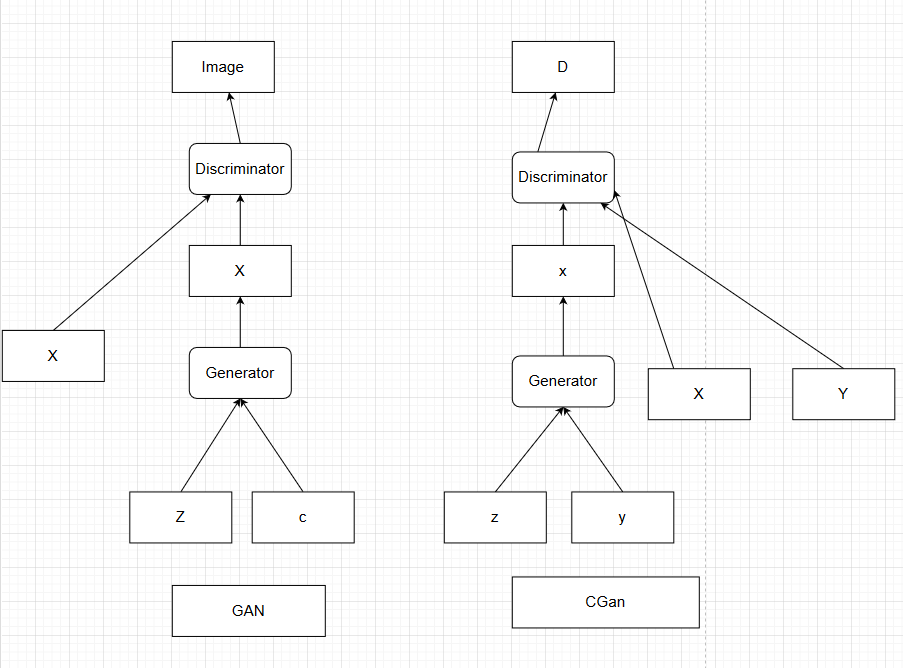
\includegraphics[width=4cm]{figures/1174042/chapter9/teori1.PNG}
           		\centering
           		\caption{Valina GAN-cGAN}
            \end{figure}
            
        \item Jelaskan dengan ilustrasi gambar sendiri arsitektur dari Age-cGAN.
		Age cGAN mempunyai 4 jaringan yang  di latih dalam 3 tahapan yaitu: Conditional GAN Training,Initial latent vector approximation,dan Latent vector optimization.
			\begin{figure}[H]
				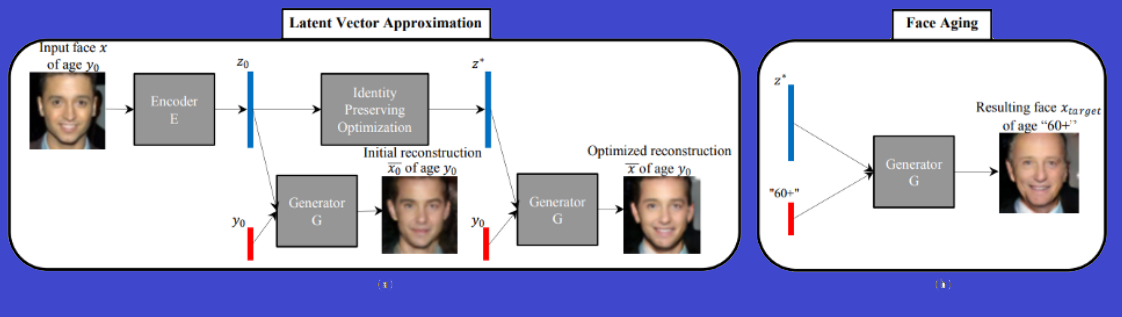
\includegraphics[width=4cm]{figures/1174042/chapter9/teori2.PNG}
            		\centering
           		\caption{Age-cGAN}
            \end{figure}
                
        \item Jelaskan dengan ilustrasi gambar sendiri arsitektur encoder network dari AgecGAN.
		Arsitektur encoder biasanya digunakan untuk mengenerate latent vector dari gambar yang akan diinputkan yang nantinya akan diteruskan ke generator.
            \begin{figure}[H]
                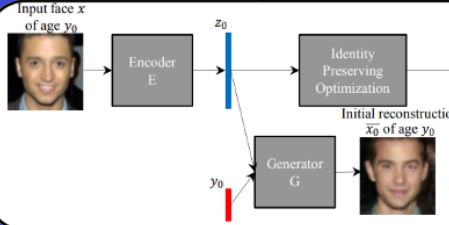
\includegraphics[width=4cm]{figures/1174042/chapter9/teori3.PNG}
                    \centering
                \caption{Encoder Age cGANr}
            \end{figure}

        \item Jelaskan dengan ilustrasi gambar sendiri arsitektur generator network dari AgecGAN.
		Arsitektur generator adalah sebuah CNN dan mengambil 100-dimensional latent vector sebagai inputannya yang akan menghasilkan gambar realistik dalam dimensi (64,64,3)
		\begin{figure}[H]
			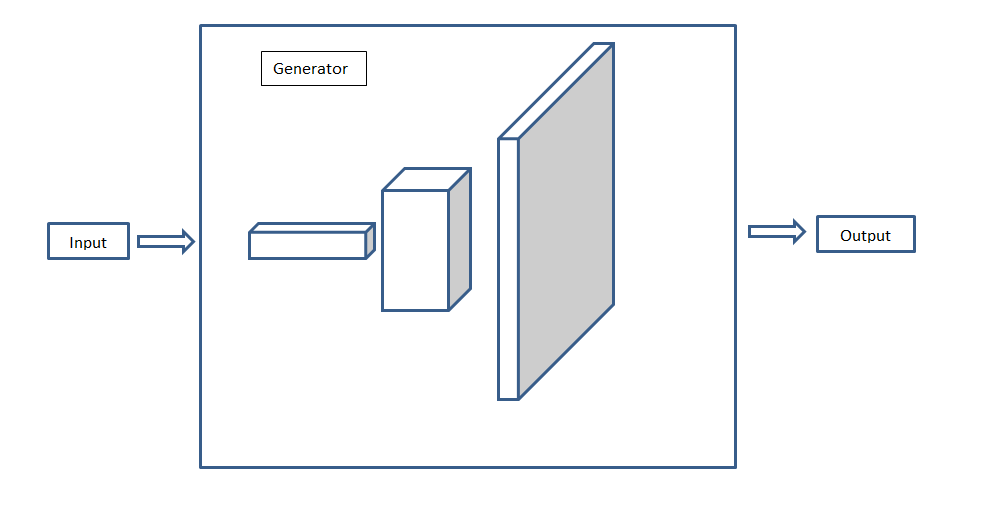
\includegraphics[width=4cm]{figures/1174042/chapter9/teori4.PNG}
            	\centering
           	\caption{Network Age cGAN}
       	\end{figure}


        \item Jelaskan dengan ilustrasi gambar sendiri arsitektur discriminator network dari Age-cGAN.
		Arsitektur diskriminator adalah CNN yang fungsinya untuk memprediksi apakah gambar yang diberikan palsu atau asli.
		\begin{figure}[H]
			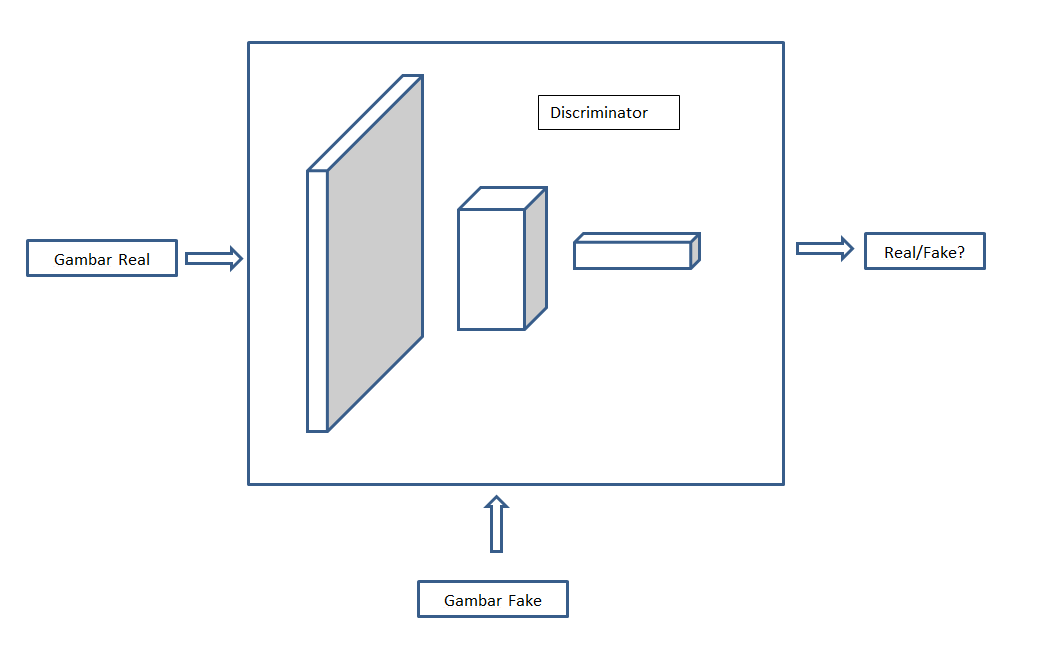
\includegraphics[width=4cm]{figures/1174042/chapter9/teori5.PNG}
            	\centering
           	\caption{Discriminator Age cGAN}
       	\end{figure}


        \item Jelaskan dengan ilustrasi gambar apa itu pre-trained Inception-ResNet-2 Model.
		Pre-Trained Network atau Transfer Learning merupakan suatu metode penyelesaian yang memanfaatkan model yang sudah dilatih terhadap suatu dataset untuk menyelesaikan masalah dengan cara menggunakan sebagai starting point, memodifikasi dan mengupdate parameternya, sehingga sesuai dengan dataset yang baru.
		\begin{figure}[H]
			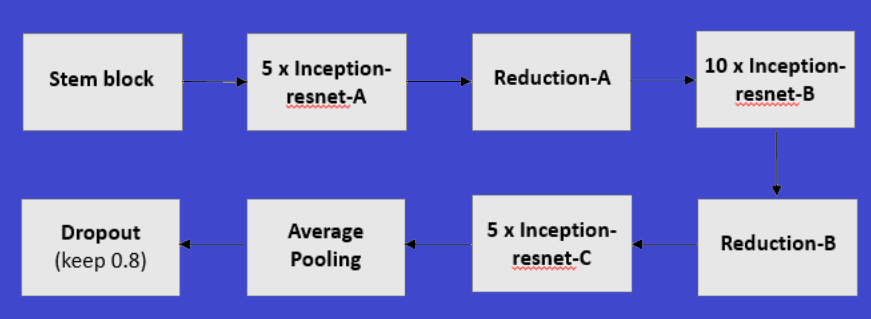
\includegraphics[width=4cm]{figures/1174042/chapter9/teori6.PNG}
            	\centering
           	\caption{Pretrained Inception ResNet}
       	\end{figure}

        \item Jelaskan dengan ilustrasi gambar sendiri arsitektur Face recognition network Age-cGAN.
		Face Recognition digunakan untuk mengenali identitas seseorang dari gambar yang diberikan.
		\begin{figure}[H]
			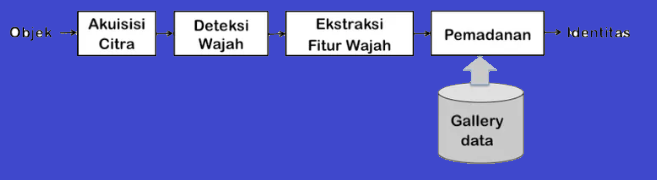
\includegraphics[width=4cm]{figures/1174042/chapter9/teori7.PNG}
            	\centering
           	 \caption{Face recognition network Age-cGAN}
       	 \end{figure}

        \item Sebutkan dan jelaskan serta di sertai contoh-contoh tahapan dari Age-cGAN.
		Pada dari Age-cGan ni terdapat 2 tahapan dengan generator dan diskriminator. dimana untuk tahap generator sendiri membutuhkan vektor laten 100 serta menghasilkan gambar yang realistis dari dimensinya. sedangkan tahap diskriminator itu tahapan dimana memprediksi gambar yang diberikan nyata atau palsu.
		\begin{figure}[H]
			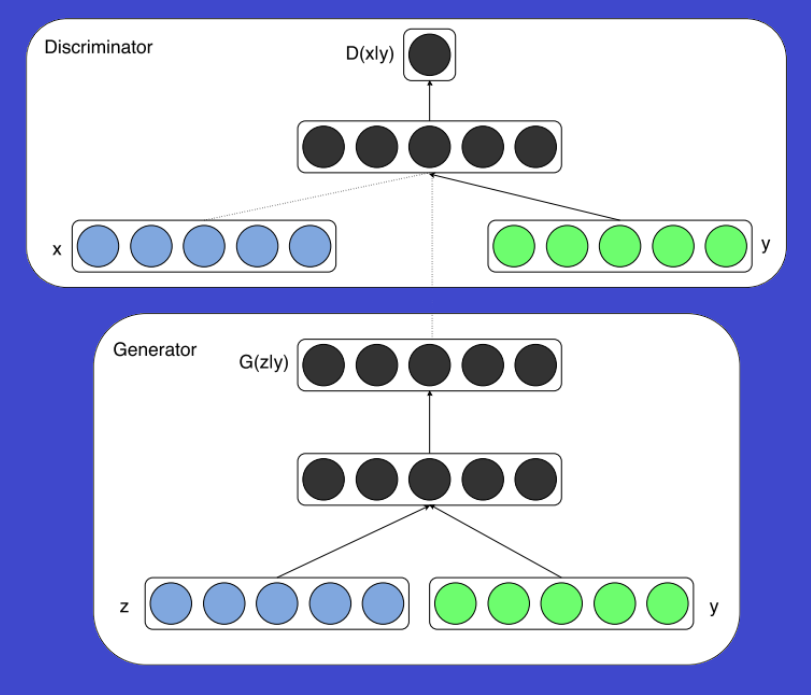
\includegraphics[width=4cm]{figures/1174042/chapter9/teori8.PNG}
            	\centering
           	 \caption{Tahap Age cGAN}
       	\end{figure}

        \item Berikan contoh perhitungan fungsi training objektif.
		Objektif Trainning ialah untuk meminimalkan loss function sebagai log likelihood function yang diberikan pada persamaan dimana D melambangkan trainning data.
		\begin{figure}[H]
			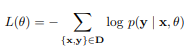
\includegraphics[width=4cm]{figures/1174042/chapter9/teori9.PNG}
            	\centering
           	 \caption{Training Objektif}
       	\end{figure}

        \item Berikan contoh dengan ilustrasi penjelasan dari Initial latent vector approximation.
		Latent vector approdimation kemampuan untuk membuat gamar yang realistis dan tajam serta menghasilkan gambar wajah pada usia target.
		\begin{figure}[H]
			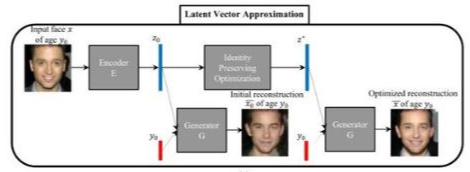
\includegraphics[width=4cm]{figures/1174042/chapter9/teori10.PNG}
            	\centering
           	 \caption{Initial Latent Vector Approximation}
       	\end{figure}

        \item Berikan contoh perhitungan latent vector optimization.
		Perhitungan lantent optimization menggunakan metode yang relatif sederhana, tergantung pada jumlah kecil parameter yang diperlukan, sehingga pada latent optimization dapat memetakan setiap gambar x dari dataset ke vektor acak dimensi rendah zi dalam ruang laten z.
		\begin{figure}[H]
			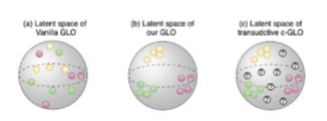
\includegraphics[width=4cm]{figures/1174042/chapter9/teori11.PNG}
            	\centering
           	\caption{Latent Vector Optimization}
        \end{figure}
           
\end{enumerate}

\subsection{Praktek}

    \begin{enumerate}
	\item Jelaskan bagaimana cara ekstrak file dataset Age-cGAN menggunakan google colab.
    Kode dibawah ini digunakan untuk membuat notebooks baru, kemudian membuat ekstraksi file dari link dataset.
	\lstinputlisting[firstline=1, lastline=4]{src/1174042/chapter9/1174042.py}

	\item Jelaskan bagaimana kode program bekerja untuk melakukan load terhadap dataset yang sudah di ekstrak, termasuk bagaimana penjelasan kode program perhitungan usia.
    Kode dibawah berfungsi untuk melakukan fungsi perhitungan usia.
	\lstinputlisting[firstline=6, lastline=31]{src/1174042/chapter9/1174042.py}

	\item Jelaskan bagaimana kode program The Encoder Network bekerja dijelaskan dengan bahawa awam dengan ilustrasi sederhana.
    Berikut adalah proses Encoder dengan vector latent Z yang berfungsi untuk mempelajari pemetaan terbalik dari gambar wajah dan kondisi usia .
	\lstinputlisting[firstline=33, lastline=73]{src/1174042/chapter9/1174042.py}

	\item Jelaskan bagaimana kode program The Generator Network bekerja dijelaskan dengan bahawa awam dengan ilustrasi sederhana.
    Proses Generator agar bekerja dengan baik dibutuhkan representasi dari gambar wajah dan vector kondisi sebagai inputan yang menghasilkan sebuah gambar.
	\lstinputlisting[firstline=75, lastline=104]{src/1174042/chapter9/1174042.py}

    \item Jelaskan bagaimana kode program The Discriminator Network bekerja dijelaskan dengan bahawa awam dengan ilustrasi sederhana.
    Berikut adalah proses Discriminator yang digunakan untuk membedakan antara gambar asli ataupun gambar palsu yang dihasilkan oleh generator.
	\lstinputlisting[firstline=116, lastline=148]{src/1174042/chapter9/1174042.py}

    \item Jelaskan bagaimana kode program Training cGAN bekerja dijelaskan dengan bahawa awam dengan ilustrasi sederhana.
    Proses Training cGAN ini dengan load file .mat pada dataset lalu epoch sebanuak 500 kali.

	\lstinputlisting[firstline=150, lastline=167]{src/1174042/chapter9/1174042.py}

    \item Jelaskan bagaimana kode program Initial dan latent vector approximation bekerja dijelaskan dengan bahawa awam dengan ilustrasi sederhana.
    Initial dan Latent Vector Approximation bekerja melakukan predicsi epoch yang telah di buat sebanyak 500 kali, dan nanti hasilnya ada di folder result.

	\lstinputlisting[firstline=169, lastline=217]{src/1174042/chapter9/1174042.py}

\end{enumerate}

\subsection{Penanganan Error}
\begin{enumerate}
	\item Tidak ada error yang terjadi
\end{enumerate}



% \input{chapters/chapter1/1174043}
% \input{chapters/chapter1/1174050}
% \section{1174057 Alit Fajar Kurniawan}
\subsection{Teori}
	\subsubsection {Sejarah Perkembangan dan Definisi Artificial Intelligence}
	Kecerdasan buatan merupakan sebuah bidang dalam ilmu computer yang begitu penting di zaman ini dan masa yang akan datang guna mewujudkan sebuah sistem computer yang begitu cerdas. Artificial Intelligence atau biasa di singkat dengan AI berasal dari bahasa latin yang dimana intelligence berarti saya paham... 
	\par Pada tahun 1955, Newell dan juga Simon telah mengembangkan The Logic Theorist, yaitu program AI pertama. Dimana program tersebut mempresentasikan sebuah masalah sebagai model pohon, lalu diselesaikan dengaan cara memilih cabang yang akan mewujudkan kesimpulan terbenar dan tepat. Program AI tersebut berdampak sangat besar dan dapat mendaji batu loncatan yang cukup penting dalam mengembangkan bidang AI \cite{baraja2008kecerdasan}.
	\par
	Masa Perkembangan AI dimulai pada awal era komputer elektronik pada tahun 1941. dimana ditemukannya alat penyimpanan dan pemrosesan informasi. kemudian dilanjutkan pada masa-masa persiapan AI yang terjadi pada tahun 1943-1956. Pada sekitaran tahun 1952-1969 merupakan masa awal perkembangan AI terjadi, dan pada tahun 1966-1974 perkembangan AI mengalami penurunan atau melambatnya proses dalam melakukan pengembangan. pada tahun 1969 sampai 10 tahun kedepan kembali terjadi perkembangan yang menciptakan inovasi sistem berbasis pengetahuan. dan sekitaran tahun 1980-an AI kembali menjadi sebuah industri yang terus berkembang sampai sekarang ini.


	\subsubsection{learning, klasifikasi, regresi dan unsupervised learning. Data set, training set dan testing set}

	\begin{enumerate}
	\item
	Definisi Supervised Learning Dan Unsupervised Learning
	\subitem
	Supervised Learning merupakan suatu pendekatan yang dimana terdapat data dan variable yang telah ditargetkan sehingga pendekatan tersebut bertujuan untuk dapat mengelompokkan sebuah data ke data yang sudah ada, beda dengan Unsupervised learning yang tidak mempunyai data, sehingga data yang ada harus di kelompokkan menjadi beberapa bagian.
	\item
	Definisi  Klasifikasi Dan Regresi
	\subitem
	Klasifikasi adalah sebuah kegiatan penggolongan atau pengelompokkan. Menurut kamus besar bahasa Indonesia yang dimana klasifikasi merupakan penyusunan sistem di dalam kelompok atau golongan berdasarkan kaidah atau standar yang telah ditetapkan. Regresi adalah sebuah metode analisis statistic yang akan digunakan untuk melihat pengaruh variable.
	\item
	Devinisi Dataset, Training Set, Dan Testing Set
	\subitem
	Dataset adalah sebuah objek yang akan mempresentasikan sebuah data dan relasinya di memory. Struktur pada dataset ini mirip dengan data yang ada di dalam database. Training set adalah bagian dari dataset yang berperan dalam membuat prediksi atau algoritma sesuai tujuan masing – masing. Testing set adalah bagian dari dataset yang akan di tes guna melihat keakuratatan atau ketepatan datanya.
	\end{enumerate}

\subsection{Praktek}
	\subsubsection{Instalasi}
	\begin{enumerate}
		\item Melakukan instalasi library scikit pada anaconda, ketik kan pip install -U scikit-learn pada terminal anaconda. 

		\begin{figure}[H]
		\centering
		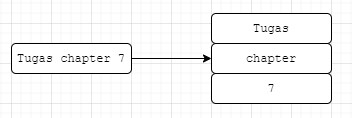
\includegraphics[width=1\textwidth]{figures/1174057/chapter1/1.png}
		\caption{Instalasi Scikit Learn}
		\label{print}
		\end{figure}

		\item Setelah selesai instalasi, pilih salah satu example dari website Scikit. 
		\begin{figure}[H]
		\centering
		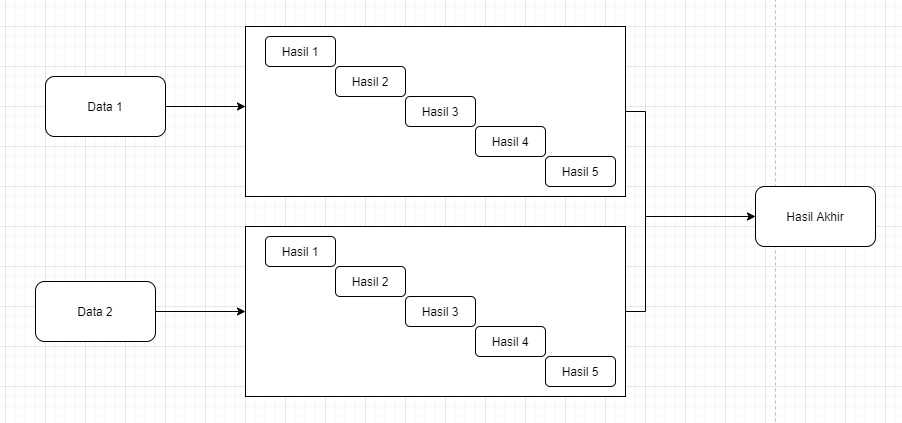
\includegraphics[width=1\textwidth]{figures/1174057/chapter1/2.png}
		\caption{Example}
		\label{print}
		\end{figure}

		\lstinputlisting[firstline=1, lastline=19]{src/1174057/chapter1/example.py}
		\par kemudian coba jalankan, lihat hasilnya
		\begin{figure}[H]
		\centering
		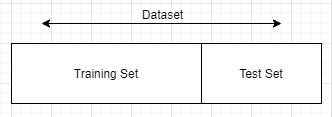
\includegraphics[width=1.5\textwidth]{figures/1174057/chapter1/3.png}
		\caption{Example}
		\label{print}
		\end{figure}

		\item latihan 2 Mencoba Loading an example dataset
		\lstinputlisting[firstline=1, lastline=9]{src/1174057/chapter1/dataset.py}
		\subitem hasil dari data digits
		\begin{figure}[H]
		\centering
		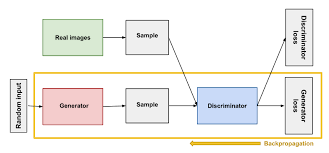
\includegraphics[width=1.5\textwidth]{figures/1174057/chapter1/4.png}
		\caption{Result Data Digits}
		\label{print}
		\end{figure}

		\subitem hasil dari digits.target
		\begin{figure}[H]
		\centering
		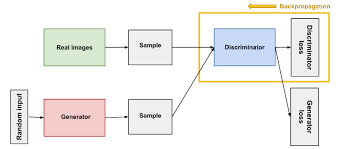
\includegraphics[width=1\textwidth]{figures/1174057/chapter1/5.png}
		\caption{Result digits.target}
		\label{print}
		\end{figure}

		\subitem hasil dari digits.image
		\begin{figure}[H]
		\centering
		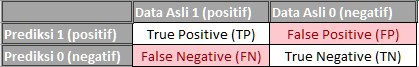
\includegraphics[width=1\textwidth]{figures/1174057/chapter1/6.png}
		\caption{Result digits.image}
		\label{print}
		\end{figure}

		\item latihan 3 Mencoba Learning and predicting
		\lstinputlisting[firstline=1, lastline=9]{src/1174057/chapter1/learning.py}
		\par kemudian coba jalankan, lihat hasilnya
		\begin{figure}[H]
		\centering
		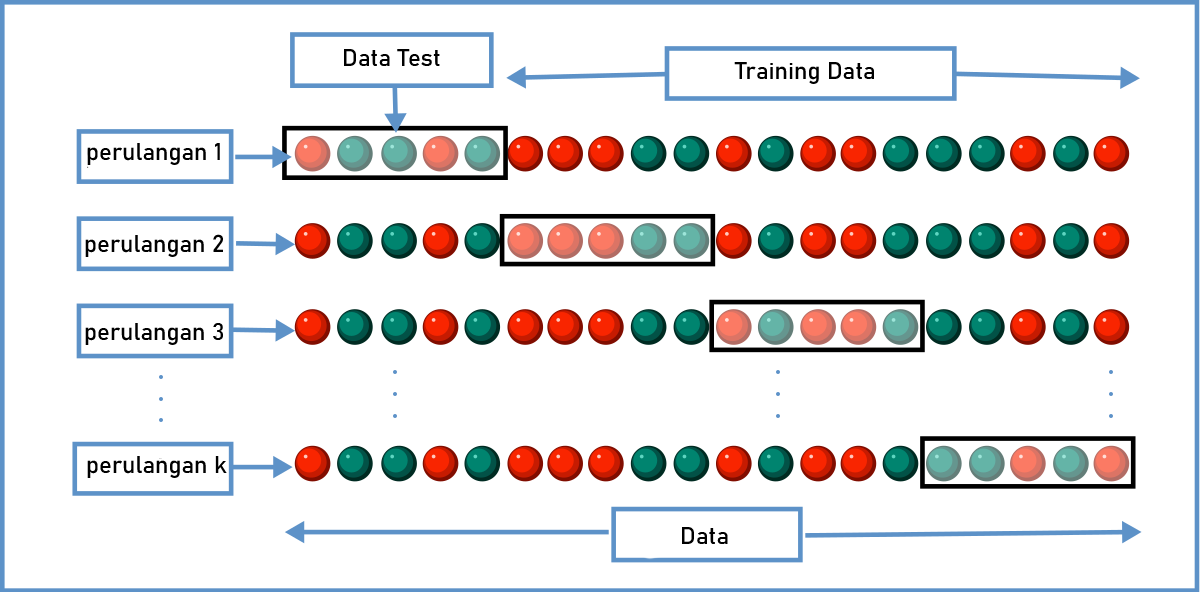
\includegraphics[width=1\textwidth]{figures/1174057/chapter1/7.png}
		\caption{Result Learning and predicting}
		\label{print}
		\end{figure}

		\item latihan 4 Mencoba Model persistence
		\lstinputlisting[firstline=1, lastline=16]{src/1174057/chapter1/modelpersistence.py}
		\par kemudian coba jalankan, lihat hasilnya
		\begin{figure}[H]
		\centering
		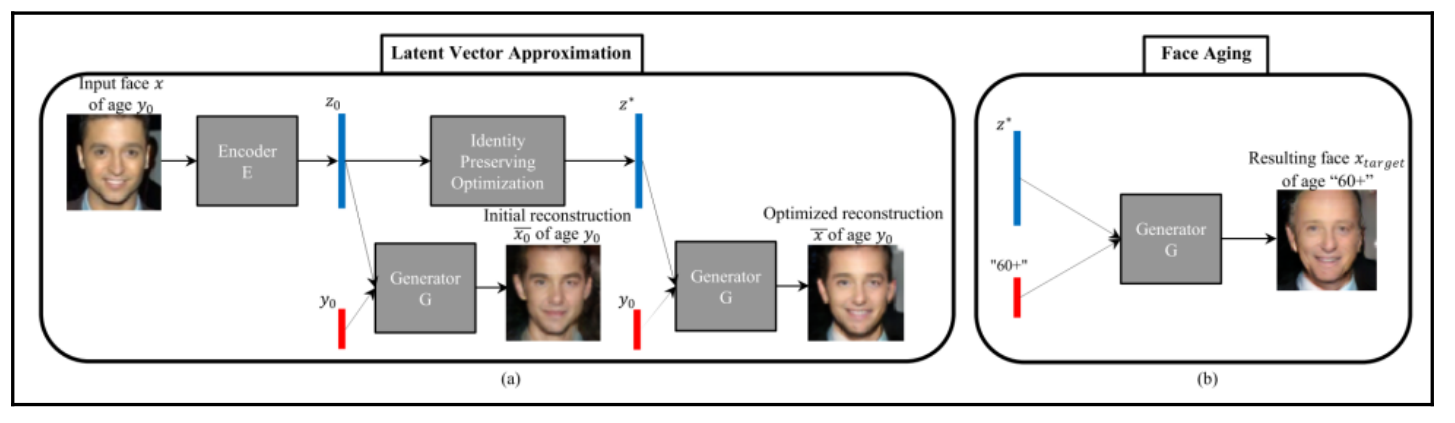
\includegraphics[width=1\textwidth]{figures/1174057/chapter1/8.png}
		\caption{Result Model persistence}
		\label{print}
		\end{figure}

		\item latihan 5 Mencoba Conventions
		\lstinputlisting[firstline=1, lastline=46]{src/1174057/chapter1/modelpersistence.py}
		\par kemudian coba jalankan, lihat hasilnya
		\begin{figure}[H]
		\centering
		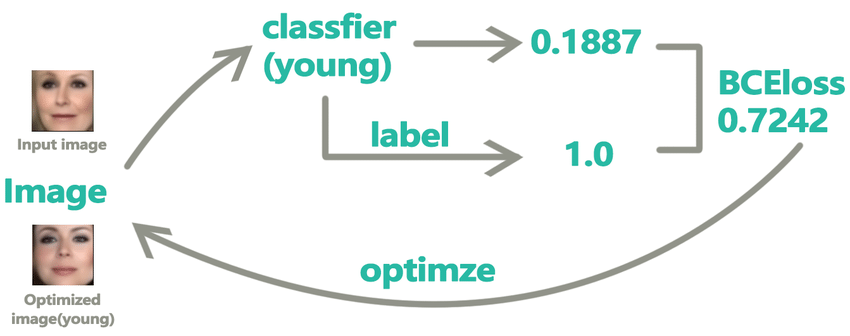
\includegraphics[width=1\textwidth]{figures/1174057/chapter1/9.png}
		\caption{Result Conventions}
		\label{print}
		\end{figure}

	\end{enumerate}

\subsection{Penanganan Error}
	\begin{enumerate}
		\item Screenshoot Error
		\begin{figure}[H]
		\centering
		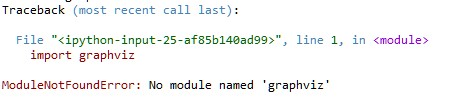
\includegraphics[width=1\textwidth]{figures/1174057/chapter1/error1.png}
		\caption{Error}
		\label{print}
		\end{figure}

		\begin{figure}[H]
		\centering
		\includegraphics[width=1\textwidth]{figures/1174057/chapter1/error2.png}
		\caption{Error}
		\label{print}
		\end{figure}

		\item Tuliskan kode dan jenis error

			\subitem is not defined, xception yang terjadi saat syntax melakukan eksekusi terhadap local name atau global name yang tidak terdefinisi.
			\subitem invalid syntax

		\item Solusi penanganan error

			\subitem Solusinya adalah memastikan variabel atau function yang dipanggil ada atau tidak salah ketik. 
			\subitem Periksa kembali syntax yang dibuat, bisa saja ada kesalahan dalam spasi.
	\end{enumerate}

\subsection{Bukti Tidak Plagiat}
	\begin{figure}[H]
		\centering
		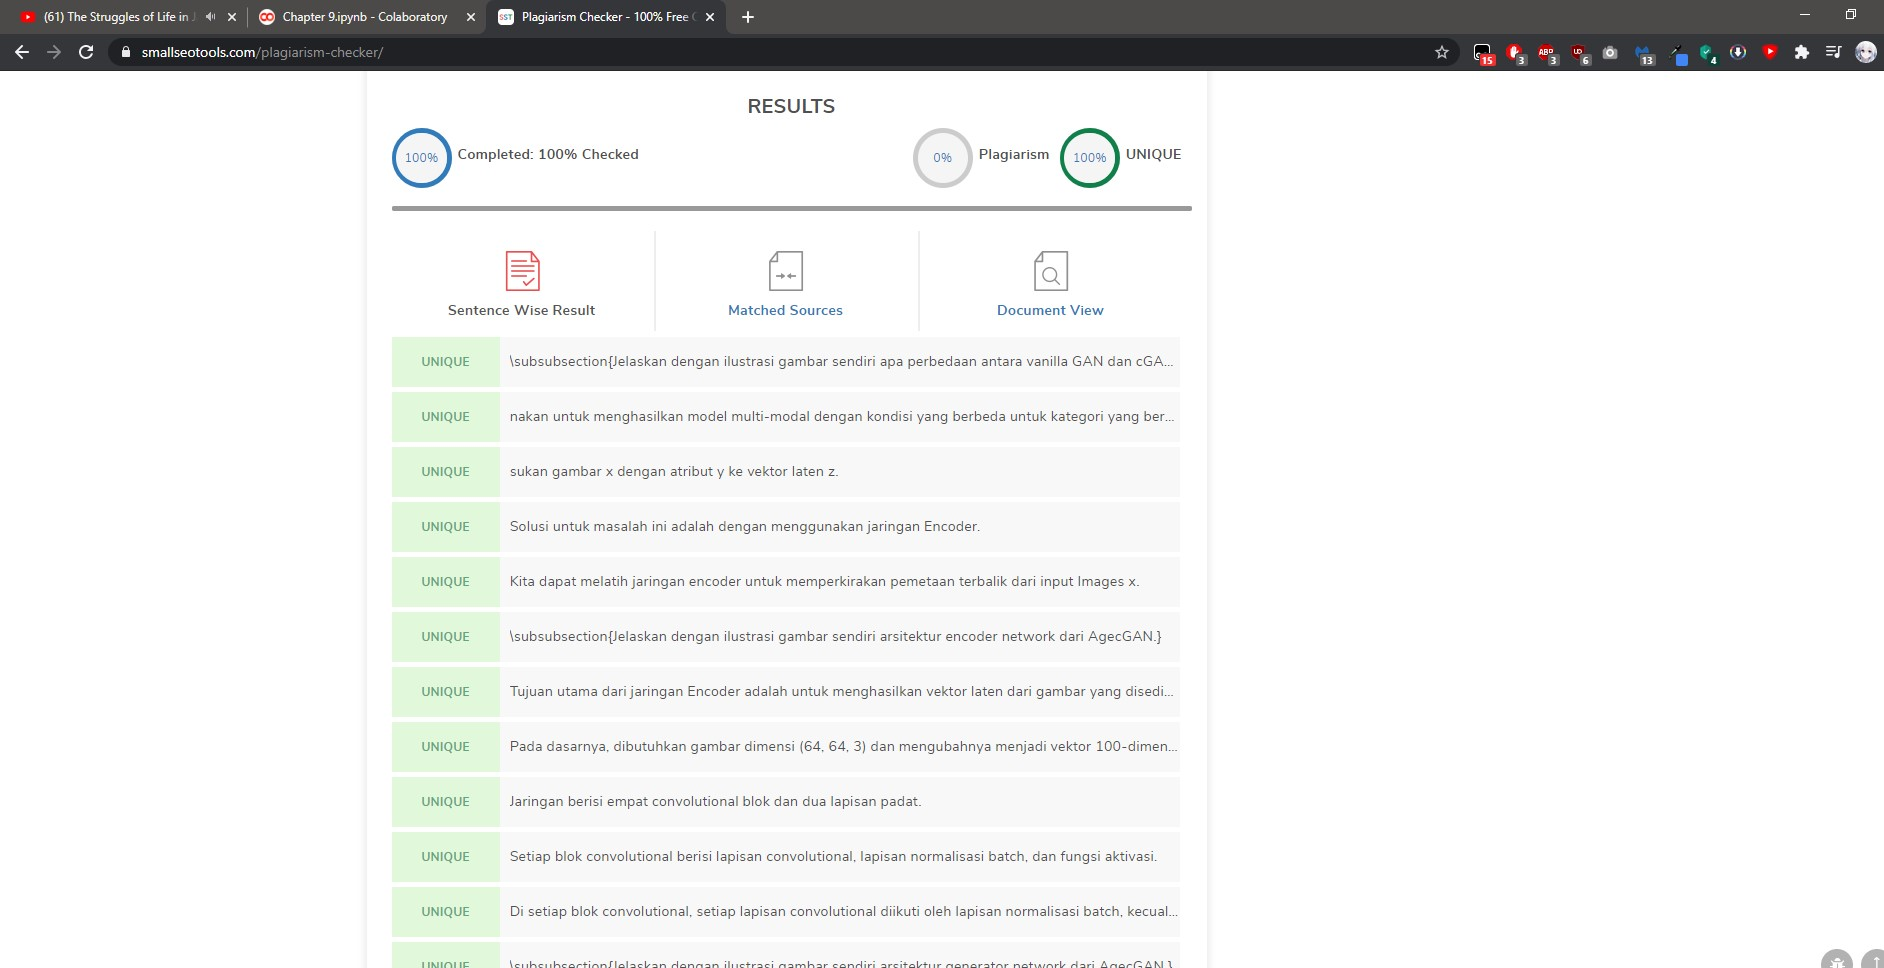
\includegraphics[width=1\textwidth]{figures/1174057/chapter1/plagiat.png}
		\caption{Plagiarisme}
		\label{print}
	\end{figure}
% \section{1174039 - Liyana Majdah Rahma}
    \subsection{Teori}
        \begin{enumerate}
            \item Jelaskan dengan ilustrasi gambar sendiri apa itu generator dengan perumpamaan anda sebagai mahasiswa sebagai generatornya.
            \par GGenerator merupakan generator yang biasanya menggunakan data yang ada untuk menghasilkan data baru, serta genarator sendiri bertujuan untuk menghasilkan data berupa video,gambar,audio dan teks.
            \begin{figure}[H]
                \includegraphics[width=4cm]{figures/1174039/chapter8/teori1.jpg}
             \centering
             \caption{Generator}
            \end{figure}

            \item Jelaskan dengan ilustrasi gambar sendiri apa itu diskriminator dengan perumpamaan dosen anda sebagai diskriminatornya
            \par Diskriminator merupakan untuk membedakan antara data nyata dan data yang dihasilkan oleh generator. pada jaringan diskriminator sendiri mencoba memasukan data ke dalamm kategori yang sudah ditentukan.

            \begin{figure}[H]
                \includegraphics[width=4cm]{figures/1174039/chapter8/teori2.jpg}
                \centering
                  \caption{Diskriminator}
            \end{figure}

            \item Jelaskan dengan ilustrasi gambar sendiri bagaimana arsitektur generator dibua
            \par Dilihat berkebalikan dengan struktur jaringan saraf pada umumnya. Pada Generator dinyatakan menerima input vektor z dan kemdian mengubahnya menjadi gambar tiga dimensi.
            \begin{figure}[H]
                \includegraphics[width=4cm]{figures/1174039/chapter8/teori3.PNG}
                \centering
                  \caption{Arsitektuk Generator}
            \end{figure}

            \item Jelaskan dengan ilustrasi gambar sendiri bagaimana arsitektur diskriminator dibuat
            \par Diskriminator merupakan jaringan klasifikasi biner yang menerima input gambar tiga dimensi dan mengeluarkan klasifikasi gambar asli. Diskriminator dilatih dengan sekumpulan data, dan sekumpulan dataset, dan dilatih untuk bisa membedakan keduanya.

            \begin{figure}[H]
                \includegraphics[width=4cm]{figures/1174039/chapter8/teori4.PNG}
                \centering
                  \caption{Arsitektur Diskriminator}
            \end{figure}

            \item Jelaskan dengan ilustrasi gambar apa itu latent space
            \par latent space adalah representasi dari data yang di kompress, untuk contohnya misalnya ada 3 gambar yaitu 2 kursi yang berebeda dan 1 meja, maka hal hal yang mirip dai kursi tersebut(ciri-ciri utamanya), seeprti itulah latent space
            \begin{figure}[H]
                \includegraphics[width=4cm]{figures/1174039/chapter8/teori5.PNG}
                \centering
                  \caption{Arsitektur Diskriminator}
            \end{figure}

            \item apa itu adversarial play
            \par Advesarial Play, berbagi data pelestarian privasi, dan vaksin rancangan. Saya menjelaskan bagaimana aspek konseptual kedua dari game keamanan menawarkan pemodelan alami paradigma untuk ini.
            \begin{figure}[H]
        \includegraphics[width=4cm]{figures/1174039/chapter8/teori6.PNG}
                \centering
             \caption{Advesarial Play}
         \end{figure}
            
            \item Jelaskan dengan ilustrasi gambar apa itu Nash equilibrium
            \par Nash equilibrium adalah konsep dalam teori permainan di mana hasil optimal dari permainan adalah di mana tidak ada insentif untuk menyimpang dari strategi awal mereka. Lebih khusus lagi, keseimbangan Nash adalah konsep teori permainan di mana hasil optimal dari permainan adalah di mana tidak ada pemain yang memiliki insentif untuk menyimpang dari strategi yang dipilihnya setelah mempertimbangkan pilihan lawan.
            \begin{figure}[H]
                \includegraphics[width=4cm]{figures/1174039/chapter8/teori7.jpg}
                \centering
                  \caption{Nash equilibrium}
            \end{figure}

            \item Sebutkan dan jelaskan contoh-contoh implementasi dari GAN
            \par Pada bidang mode, seni, dan iklan, GAN dapar digunakan untuk membuat foto-foto model fashion imajinier tanpa perlu menyewa model. Pada bidang sains GAN dapat meningkatkan citra astronomi dan mensimulasikan pelensaan gravitasi untuk penelitian materi gelap.

            \item Berikan contoh dengan penjelasan kode program beserta gambar arsitektur untuk membuat generator(neural network) dengan sebuah input layer, tiga hidden layer(dense layer), dan satu output layer(reshape layer)
\begin{verbatim}
gen=Sequential() #Inisiasi dari sequensial
gen.add(Dense(units=200,input\_dim=np.shape(train\_input)[1])) #Menambah dense layer dengan batch size 200 dan input dim dari input
gen.add(Dense(units=400))#Menambah dense layer dengan batch size 400 dan input dim 100
gen.add(Dense(units=784, activation='tanh')) #Menambah dense layer dengan batch size 784 dan aktivasi metode tanh
gen.compile(loss='binary\_crossentropy', optimizer=adam\_optimizer()) #Menkompilasi hasil penambahan setiap dense
 gen.summary() #Memproses data yang sudah disetting dan menampilkannya
\end{verbatim}    
            \par Pada contoh tersebut, data akan diambil dari hasil proses sebelumnya yaitu proses ekstrasi data gambar. Dari contoh ini, terdapat 3 layer dense, 1 input layer dan 1 output layer. Dari input layer nanti akan dimasukkan terlebih dahulu ke dense layer pertama lalu diproses oleh 2 layer selanjutnya dan terakhir akan ditampilkan oleh layer output.
            \begin{figure}[H]
                \includegraphics[width=4cm]{figures/1174039/chapter8/teori9.PNG}
                \centering
                  \caption{Hasil Arsitektuk Generator}
            \end{figure}

            \item Berikan contoh dengan ilustrasi dari arsitektur dikriminator dengan sebuath input layer, 3 buah hidden layer, dan satu output layer.
\begin{verbatim}
diskrim=Sequential()#Inisiasi dari sequensial
diskrim.add(Dense(units=784,input\_dim=np.shape(train\_input)[1]))#Menambah dense layer dan input dim dari layer
diskrim.add(Dense(units=400)) #Mensetting Dense
diskrim.add(Dense(units=200, activation='sigmoid')) #Mensetting dense dan melakukan aktivasi dengan metode sigmoid
diskrim.compile(loss='binary\_crossentropy', optimizer=adam\_optimizer())#Menkompilasi hasil penambahan setiap dense
diskrim.summary()#Memproses data yang sudah disetting dan menampilkannya
\end{verbatim}
            \par Pada contoh tersebut, data akan diambil dari hasil proses sebelumnya yaitu proses ekstrasi data gambar. Dari contoh ini, terdapat 3 layer dense, 1 input layer dan 1 output layer. Pada proses ini, seluruh data akan dibandingkan dengan data sebelumnya yaitu dari generator dan dari data aslinya yang sudah dijadikan data vector. 
            \begin{figure}[H]
                \includegraphics[width=4cm]{figures/1174039/chapter8/teori10.PNG}
                \centering
                  \caption{Hasil Arsitektur Generator}
            \end{figure}
            
            \item Jelaskan bagaimana kaitan output dan input antara generator dan diskriminator tersebut. Jelaskan kenapa inputan dan outputan seperti itu
            \par Pada kedua metode tersebut, akan disebutkan berapa akurasi dari setiap metode. Pada setiap metode tersebut (Discriminator dan generator) akan dilakukan pelatihan dan akan dibandingkan hasilnya. Generator akan menghasilkan data baru sesuai dengan hasil latihan dan dari data tersebut, discriminator akan membandingkan dengan data set apakah data tersebut "asli" atau tidak.
            
            \item Jelaskan apa perbedaan antara Kullback-Leibler divergence (KL divergence)/relative entropy, Jensen-Shannon(JS) divergence / information radius(iRaD) / total divergence to the average dalam mengukur kualitas dari model
            \par relative entropy adalah ukuran dari bagaimana satu distribusi probabilitas berbeda dari yang kedua, distribusi probabilitas referensi, Divergensi Jensen-Shannon adalah ukuran divergensi berprinsip yang selalu terbatas untuk variabel acak terbatas.

            \item Jelaskan apa itu fungsi objektif yang berfungsi untuk mengukur kesamaan antara gambar yang dibuat dengan yang asli.
            \par Fungsi objektif adalah fungsi yang digunakan sebagai penujuk berapa nilai kesamaan anatara gambar yang dibuat dengan yang asli

            \item Jelaskan apa itu scoring algoritma selain mean square error atau cross entropy seperti The Inception Score dan The Frechet Inception distance.
            \par Inception Score digunakan untuk mengukur seberapa realistis output dari GAN, dimana ada dua parameter, yaitu : gambarnya punya variasi dan setiap gambar jelas terlihat seperti sesuatu. Frechet Inception Distance adalah ukuran kesamaan antara dua dataset gambar. Itu terbukti berkorelasi baik dengan penilaian manusia terhadap kualitas visual dan paling sering digunakan untuk mengevaluasi kualitas sampel Generative Adversarial Networks. FID dihitung dengan menghitung jarak Fréchet antara dua Gaussians dipasang ke representasi fitur dari jaringan Inception.
            
            \item Jelaskan kelebihan dan kekurangan GAN
            \begin{itemize}
              \item Kelebihan 
              \begin{enumerate}
               
                \item GAN Menghasilkan data baru yang bisa hampir mirip dengan data asli. Karena hasil pelatihannya, GAN dapat menghasilkan data gambar, teks, audio, dan video yang dapat dibilang hampir mirip dengan yang aslinya. Berkat hal tersebut, GAN dapat digunakan dalam sistem marketing, e-commerce, games,iklan, dan industri lainnya
                \item GAN mempelajari representasi data secara internal sehingga beberapa masalah pada machine learning dapat diatasi dengan mudah
                \item Discriminator yang sudah dilatih dapat menjadi sebuah classifier atau pendeteksi jika data sudah sesuai. Karena Discriminator yang akan menjadi tidak efisien berkat seringnya dilatih
                \item GAN dapat dilatih menggunakan data yang belum dilabeled
              
            \end{enumerate}
              \item Kekurangan
              \begin{enumerate}  
                \item Data saat diproses oleh metode gan tidak konvergensi
                \item Jenis sampel yang dihasilkan oleh generator terbatas karena modenya terbatas
                \item Ketidak seimbangnya antara generator dan discriminator dapat menyebabkan overfitting atau terlalu dekat dengan hasil sampel
                \item Sangat sensitif dengan data yang sudah diinisiasi sebelumnya
              \end{enumerate}
            \end{itemize}

        \end{enumerate}

        \subsection{Praktek}
        \begin{enumerate}
        \item Jelaskan apa itu 3D convolutions
        Konvolusi 3D. Konvolusi 3D menerapkan filter 3 dimensi ke dataset dan filter bergerak 3 arah (x, y, z) untuk menghitung representasi fitur level rendah. Bentuk output mereka adalah ruang volume 3 dimensi seperti kubus atau kuboid.
        
        \item Jelaskan dengan kode program arsitektur dari generator networknya, beserta penjelasan input dan output dari generator network.
        \lstinputlisting{src/1174039/chapter8/no2.py}
        generator ialah g\_loss, Bentuk jaringan Generator dapat dilihat berkebalikan dengan struktur jaringan saraf pada umumnya. Jaringan Generator menerima input sebuah vektor angka z, kemudian mengubahnya menjadi output gambar tiga dimensi.
        
        \item Jelaskan dengan kode program arsitektur dari diskriminator network, beserta penjelasan input dan outputnya.
        \lstinputlisting{src/1174039/chapter8/no3.py}
        diskrimanator adalah d\_loss, Jaringan Discriminator merupakan jaringan klasifikasi biner yang menerima input gambar tiga dimensi dan mengeluarkan klasifikasi menyatakan input gambar adalah gambar asli dari dataset atau merupakan gambar buatan Generator.
        
        \item Jelaskan proses training 3D-GANs
        proses training 3D gan yaitu dengan melakukan epoch sebanyak yang ditentukan.
        
        \item Jelaskan bagaimana melakukan settingan awal chapter 02 untuk memenuhi semua kebutuhan sebelum melanjutkan ke tahapan persiapan data.
        1. clone github										 2. download dataset 									3. buat folder baru logs dan results
        
        \item Jelaskan tentang dataset yang digunakan, dari mulai tempat unduh, cara membuka dan melihat data. Sampai deskripsi dari isi dataset dengan detail penjelasan setiap folder/file yang membuat orang awam paham.
        dataset digunakan yaitu 3DShapeNets yang berisi model model bentuk benda dll, folder train berisi train dan folder test berisi data testing. dan semua data tersebut di simpan didalam folder volumetric\_data 
        
        \item Jelaskan apa itu voxel dengan ilustrasi dan bahasa paling awam
        Volume pixel atau voxel adalah titik dalam ruang tiga dimensi. Sebuah voxel mendefinisikan posisi dengan tiga koordinat dalam arah x, y, dan z. Sebuah voxel adalah unit dasar untuk mewakili gambar 3D
        
        \item Visualisasikan dataset tersebut dalam tampilan visual plot, jelaskan cara melakukan visualisasinya
        1. import library									   2. load data file .mat  								  3. lalu read memakai matplotlib
        
        \item buka file run.py jelaskan perbaris kode pada fungsi untuk membuat generator yaitu build generator.
        membuat generator yaitu dengan ketentukan gen sebagai variabel dan membuat fungsi atau variabel gen\_model lalu dilakukan return
        
        \item jelaskan juga fungsi untuk membangun diskriminator pada fungsi build discriminator.
        membangun diskriminator berfungsi untuk mendefenisikan seluruh gambar yang sudah di load generator sebagai gambar fake dan real
        
        \item Jelaskan kode program
        \lstinputlisting{src/1174039/chapter8/1.py}
        Jika interpreter python menjalankan if name main  sebagai program utama, itu ialah menetapkan variabel name  untuk memiliki nilai main. Jika file ini sedang diimpor dari modul lain, name akan ditetapkan ke nama modul. Nama modul tersedia sebagai nilai untuk name variabel global.
        
        \item Jelaskan kode program 
        \lstinputlisting{src/1174039/chapter8/2.py}
        artinya adalah load dataset yang hanya dalam folder chair data train
        
        \item Jelaskan kode program 
        \lstinputlisting{src/1174039/chapter8/3.py}
        disini menggunakan Adam sebagai algoritma pengoptimalan dan binary\_crossentropy sebagai kerugian loss. 
        
        \item Jelaskan kode program 
        \lstinputlisting{src/1174039/chapter8/4.py}
        ini artinya ialah kita memasukkan random vector kedalam generator model lalu membagi 2 yaitu generated example dan real example, dan meneruskan ke diskriminator model sebagai real atau fake
        
        \item Jelaskan kode program 
        \lstinputlisting{src/1174039/chapter8/5.py}
        ini melakukan load data pada dataset
        
        \item Jelaskan kode program 
        \lstinputlisting{src/1174039/chapter8/6.py}
        ini berfungsi untuk membuat tensorboard yang nantinya bisa diakses melalui localhost
        
        \item Jelaskan kode program 
        \lstinputlisting{src/1174039/chapter8/7.py}
        fungsi ini ialah untuk melakukan reshape agar shape yang dihasilkan tidak terlalu besar.
        
        \item Jelaskan kode program 
        \lstinputlisting{src/1174039/chapter8/8.py}
        karena jika epoch semakin banyak maka kualiatas training yang dihasilkan akan semakin baik
        
        \item Jelaskan kode program 
        \lstinputlisting{src/1174039/chapter8/9.py}
        batch adalah jumlah file yang akan di training
        
        \item Jelaskan kode program 
        \lstinputlisting{src/1174039/chapter8/10.py}
        ini adalah untuk membuat gambar bersih dari noise dan juga menyesuaikan shape
        
        \item Jelaskan kode program 
        \lstinputlisting{src/1174039/chapter8/11.py}
        ialah membuat sample gambar palsu yang akan diteruskan ke diskriminator
        
        \item Jelaskan kode program 
        \lstinputlisting{src/1174039/chapter8/12.py}
        diskriminator bisa load gambar fake dan real dari generator, oleh karena itu ada generator loss dan diskriminator loss untuk melihat seberapa baik kualitas yang dihasilkan
        
        \item Jelaskan kode program 
        \lstinputlisting{src/1174039/chapter8/13.py}
        dengan melakukan print g\_loss untuk generator dan juga d\_loss untuk diskriminator
        
        \item Jelaskan kode program 
        \lstinputlisting{src/1174039/chapter8/14.py}
        mengapa ada perulangan karena untuk melakukan perbandingan dari hasil yang sudah didapat.
        
        \item Jelaskan kode program 
        \lstinputlisting{src/1174039/chapter8/15.py}
        TensorBoard adalah sebuah aplikasi web localhost untuk memeriksa dan menyelesaikan grafik dari hasil TensorFlow.
        
        \item Jelaskan kode program 
        \lstinputlisting{src/1174039/chapter8/16.py}
        File H5 adalah file data yang disimpan dalam Format Data Hirarki (HDF). Ini berisi array multidimensi data ilmiah
        
        \item Jelaskan kode program 
        \lstinputlisting{src/1174039/chapter8/17.py}
        ini adalah tahap akhir untuk melakukan testing dari model yang telah dibuat dan buat model dari yang sudah di create sebelumnya yaitu generator dan diskriminator.
        
        \begin{figure}[H]
        \centering
        \includegraphics[width=4cm]{figures/1174039/chapter8/1.png}
        \caption{Result}
        \end{figure}
        
        \begin{figure}[H]
        \centering
        \includegraphics[width=4cm]{figures/1174039/chapter8/2.png}
        \caption{Result} 
        \end{figure}
        
        \begin{figure}[H]
          \centering
          \includegraphics[width=4cm]{figures/1174039/chapter8/3.png}
        \caption{Result}
 
        \end{figure}
        
        \begin{figure}[H]
        \centering
        \includegraphics[width=4cm]{figures/1174039/chapter8/4.jpg}
        \caption{Result}
        \end{figure}
        
        
        \end{enumerate}

% \chapter{Chapter 2}
% %\input{chapters/chapter2/1174006}
% \section{1174042 Faisal Najib Abdullah}

\subsection{Teori}
\begin{enumerate}

        \item Jelaskan dengan ilustrasi gambar sendiri apa perbedaan antara vanilla GAN dan cGAN.
		Generator dan Disciminator pada Vanilla GAN adalah pembelajaran multi-layer yang sederhana, dimana algoritmanya sederhana yang mencoba untuk mengoptimasi persamman matematika menggunakan penurunan gradien stokastik. Sedangkan cGAN dapat dideskripsikan sebagai deep learing pada parameter kondisional diberlakukan.
			\begin{figure}[H]
            	\includegraphics[width=4cm]{figures/1174042/chapter9/teori1.PNG}
           		\centering
           		\caption{Valina GAN-cGAN}
            \end{figure}
            
        \item Jelaskan dengan ilustrasi gambar sendiri arsitektur dari Age-cGAN.
		Age cGAN mempunyai 4 jaringan yang  di latih dalam 3 tahapan yaitu: Conditional GAN Training,Initial latent vector approximation,dan Latent vector optimization.
			\begin{figure}[H]
				\includegraphics[width=4cm]{figures/1174042/chapter9/teori2.PNG}
            		\centering
           		\caption{Age-cGAN}
            \end{figure}
                
        \item Jelaskan dengan ilustrasi gambar sendiri arsitektur encoder network dari AgecGAN.
		Arsitektur encoder biasanya digunakan untuk mengenerate latent vector dari gambar yang akan diinputkan yang nantinya akan diteruskan ke generator.
            \begin{figure}[H]
                \includegraphics[width=4cm]{figures/1174042/chapter9/teori3.PNG}
                    \centering
                \caption{Encoder Age cGANr}
            \end{figure}

        \item Jelaskan dengan ilustrasi gambar sendiri arsitektur generator network dari AgecGAN.
		Arsitektur generator adalah sebuah CNN dan mengambil 100-dimensional latent vector sebagai inputannya yang akan menghasilkan gambar realistik dalam dimensi (64,64,3)
		\begin{figure}[H]
			\includegraphics[width=4cm]{figures/1174042/chapter9/teori4.PNG}
            	\centering
           	\caption{Network Age cGAN}
       	\end{figure}


        \item Jelaskan dengan ilustrasi gambar sendiri arsitektur discriminator network dari Age-cGAN.
		Arsitektur diskriminator adalah CNN yang fungsinya untuk memprediksi apakah gambar yang diberikan palsu atau asli.
		\begin{figure}[H]
			\includegraphics[width=4cm]{figures/1174042/chapter9/teori5.PNG}
            	\centering
           	\caption{Discriminator Age cGAN}
       	\end{figure}


        \item Jelaskan dengan ilustrasi gambar apa itu pre-trained Inception-ResNet-2 Model.
		Pre-Trained Network atau Transfer Learning merupakan suatu metode penyelesaian yang memanfaatkan model yang sudah dilatih terhadap suatu dataset untuk menyelesaikan masalah dengan cara menggunakan sebagai starting point, memodifikasi dan mengupdate parameternya, sehingga sesuai dengan dataset yang baru.
		\begin{figure}[H]
			\includegraphics[width=4cm]{figures/1174042/chapter9/teori6.PNG}
            	\centering
           	\caption{Pretrained Inception ResNet}
       	\end{figure}

        \item Jelaskan dengan ilustrasi gambar sendiri arsitektur Face recognition network Age-cGAN.
		Face Recognition digunakan untuk mengenali identitas seseorang dari gambar yang diberikan.
		\begin{figure}[H]
			\includegraphics[width=4cm]{figures/1174042/chapter9/teori7.PNG}
            	\centering
           	 \caption{Face recognition network Age-cGAN}
       	 \end{figure}

        \item Sebutkan dan jelaskan serta di sertai contoh-contoh tahapan dari Age-cGAN.
		Pada dari Age-cGan ni terdapat 2 tahapan dengan generator dan diskriminator. dimana untuk tahap generator sendiri membutuhkan vektor laten 100 serta menghasilkan gambar yang realistis dari dimensinya. sedangkan tahap diskriminator itu tahapan dimana memprediksi gambar yang diberikan nyata atau palsu.
		\begin{figure}[H]
			\includegraphics[width=4cm]{figures/1174042/chapter9/teori8.PNG}
            	\centering
           	 \caption{Tahap Age cGAN}
       	\end{figure}

        \item Berikan contoh perhitungan fungsi training objektif.
		Objektif Trainning ialah untuk meminimalkan loss function sebagai log likelihood function yang diberikan pada persamaan dimana D melambangkan trainning data.
		\begin{figure}[H]
			\includegraphics[width=4cm]{figures/1174042/chapter9/teori9.PNG}
            	\centering
           	 \caption{Training Objektif}
       	\end{figure}

        \item Berikan contoh dengan ilustrasi penjelasan dari Initial latent vector approximation.
		Latent vector approdimation kemampuan untuk membuat gamar yang realistis dan tajam serta menghasilkan gambar wajah pada usia target.
		\begin{figure}[H]
			\includegraphics[width=4cm]{figures/1174042/chapter9/teori10.PNG}
            	\centering
           	 \caption{Initial Latent Vector Approximation}
       	\end{figure}

        \item Berikan contoh perhitungan latent vector optimization.
		Perhitungan lantent optimization menggunakan metode yang relatif sederhana, tergantung pada jumlah kecil parameter yang diperlukan, sehingga pada latent optimization dapat memetakan setiap gambar x dari dataset ke vektor acak dimensi rendah zi dalam ruang laten z.
		\begin{figure}[H]
			\includegraphics[width=4cm]{figures/1174042/chapter9/teori11.PNG}
            	\centering
           	\caption{Latent Vector Optimization}
        \end{figure}
           
\end{enumerate}

\subsection{Praktek}

    \begin{enumerate}
	\item Jelaskan bagaimana cara ekstrak file dataset Age-cGAN menggunakan google colab.
    Kode dibawah ini digunakan untuk membuat notebooks baru, kemudian membuat ekstraksi file dari link dataset.
	\lstinputlisting[firstline=1, lastline=4]{src/1174042/chapter9/1174042.py}

	\item Jelaskan bagaimana kode program bekerja untuk melakukan load terhadap dataset yang sudah di ekstrak, termasuk bagaimana penjelasan kode program perhitungan usia.
    Kode dibawah berfungsi untuk melakukan fungsi perhitungan usia.
	\lstinputlisting[firstline=6, lastline=31]{src/1174042/chapter9/1174042.py}

	\item Jelaskan bagaimana kode program The Encoder Network bekerja dijelaskan dengan bahawa awam dengan ilustrasi sederhana.
    Berikut adalah proses Encoder dengan vector latent Z yang berfungsi untuk mempelajari pemetaan terbalik dari gambar wajah dan kondisi usia .
	\lstinputlisting[firstline=33, lastline=73]{src/1174042/chapter9/1174042.py}

	\item Jelaskan bagaimana kode program The Generator Network bekerja dijelaskan dengan bahawa awam dengan ilustrasi sederhana.
    Proses Generator agar bekerja dengan baik dibutuhkan representasi dari gambar wajah dan vector kondisi sebagai inputan yang menghasilkan sebuah gambar.
	\lstinputlisting[firstline=75, lastline=104]{src/1174042/chapter9/1174042.py}

    \item Jelaskan bagaimana kode program The Discriminator Network bekerja dijelaskan dengan bahawa awam dengan ilustrasi sederhana.
    Berikut adalah proses Discriminator yang digunakan untuk membedakan antara gambar asli ataupun gambar palsu yang dihasilkan oleh generator.
	\lstinputlisting[firstline=116, lastline=148]{src/1174042/chapter9/1174042.py}

    \item Jelaskan bagaimana kode program Training cGAN bekerja dijelaskan dengan bahawa awam dengan ilustrasi sederhana.
    Proses Training cGAN ini dengan load file .mat pada dataset lalu epoch sebanuak 500 kali.

	\lstinputlisting[firstline=150, lastline=167]{src/1174042/chapter9/1174042.py}

    \item Jelaskan bagaimana kode program Initial dan latent vector approximation bekerja dijelaskan dengan bahawa awam dengan ilustrasi sederhana.
    Initial dan Latent Vector Approximation bekerja melakukan predicsi epoch yang telah di buat sebanyak 500 kali, dan nanti hasilnya ada di folder result.

	\lstinputlisting[firstline=169, lastline=217]{src/1174042/chapter9/1174042.py}

\end{enumerate}

\subsection{Penanganan Error}
\begin{enumerate}
	\item Tidak ada error yang terjadi
\end{enumerate}



% \section{1174035 Luthfi Muhammad Nabil}
Kecerdasan buatan merupakan kecerdasan yang dimasukkan ke sistem yang dapat diatur untuk kepentingan ilmiah. Kecerdasan buatan biasa disebut AI (Artificial Intelligence) yang didefinisikan sebagai kecerdasan ilmiah. AI memiliki kemampuan untuk menerjemahkan data dari luar, dan mempelajari data tersebut untuk dipelajari demi mencapai tujuan dan melakukan tugas tertentu sesuai hasil adaptasi berdasarkan data yang didapat. 

\subsection{Sejarah dan perkembangaan Kecerdasan Buatan}
AI mulai berkembang sesuai dengan konsep yang dikemukakan pada awal abad 17, Rene Descartes menyebutkan bahwa tubuh hewan bukanlah apa-apa melainkan mesin-mesin yang rumit. Lalu Blaise Pascal menciptakan mesin perhitungan digital mekanis pertama pada 1642. Selanjutnya pada abad ke 19, Charles Babbage dan Ada Lovelace menciptakan sebuah mesin penghitung mekanis yang dapat diprogram.

Pada tahun 1950-an, Program AI pertama yang sudah dapat difungsikan telah ditulis pada 1951 untuk menjalankan mesin Ferranti Mark I di University of Manchester yang merupakan sebuah program permainan naskah yang ditulis oleh Christopher Strachey. John McCarthy menyebutkan istilah "kecerdasan buatan" pada konferensi pertama yang disediakan untuk persoalan ini. Dilanjut pada tahun 1956, Beliau menemukan bahasa pemrograman yang bernama Lisp.

Jaringan saraf mulai digunakan secara luas pada tahun 1980-an, dimana algoritma perambatan balik pertama kali dijelaskan oleh Paul John Werbos pada tahun 1974. Selanjutnya di tahun 1982, para ahli fisika menganalisis sifat dari penyimpanan dan optimasi pada jaringan saraf menggunakan sistem statistika. Lalu dilanjutkan pada tahun 1985 sedikitnya empat kelompok riset menemukan algoritma pembelajaran propagansi balik. Algoritma ini berhasil diimplementasikan ke ilmu komputer dan psikologi. Dan pada tahun 1990, ditandai perolehan besar dalam berbagai bidang AI dan demonstrasi dari berbagai aplikasi yang sudah mengimplementasi. Seperti Deep Blue, sebuah komputer dari permainan catur yang dapat mengalahkan Garry Kasparov dalam sebuah pertandingan 6 game yang terkenal pada 1997. 

\subsection{Supervised Learning}
Supervised learning adalah kondisi yang menggunakan variabel input dan output untuk dapat dilakukan pemetaan input output yang sudah didapat. Disebud Supervised Learning karena proses dari pembelajaran algoritma dari pembelajan yang disumberkan dengan dataset dapat dipikirkan seperti seorang guru yang mengawasi proses pembelajaran. Proses pembelajaran dari algoritma akan berhenti saat algoritma sudah mendapatkan level dari performansi yang dapat diteriima.
\hfill\break
Masalah dari Supervised learning dapat dikelompokkan menjadi masalah dengan regresi dan klasifikasi
\begin{itemize}
	\item Klasifikasi : Masalah dalam klasifikasi yang dimana output dari variable itu adalah kategori, seperti "Laki - laki" atau "Perempuan, dan "Muda" dan "Tua"
	\item Regresi : Masalah dalam regresi adalah jika pengeluaran dari variabel adalah sebuah nilai asli, seperti "suhu", dan "tinggi"
\end{itemize}

\subsection{Unsupervised Learning}
Unsupervised learning adalah kondisi dimana kamu hanya memiliki input data tanpa memiliki variabel output yang sesuai. Tujuan dari unsupervised learning adalah untuk memodelkan distribusi pada data untuk mengetahui lebih lanjut mengenai data. Disebut unsupervised learning karena pada metode ini, tidak ada jawaban yang tepat dan tidak ada pengarah. Sehingga algoritma akan ditinggalkan sesuai rancangan demi menemukan dan dapat mengolah data yang menarik pada saat yang akan datang. 

\subsection{Jenis - Jenis Dataset}
Dataset merupakan objek yang merepresentasikan data dan relasinya di memor. Strukturnya dapat mirip sesuai dengan struktur yang ada pada database namun bisa diubah sesuai dengan kebutuhan. Dataset juga berisi koleksi dari tabel data dan relasi data.
\begin{itemize}
	\item Training set : merupakan sebuah dataset yang digunakan untuk kepentingan pembelajaran. Kepentingan tersebut akan disesuaikan dengan parameter yang ada. 
	\item Test dataset : adalah sebuah dataset yang bersifat independen dibandingkan dengan training dataset, namun mengikuti probabilitas distribusi yang sama dengan training dataset. Jika model sudah sesuai dengan training dataset maka dataset sudah dapat disesuaikan dengan test dataset. Penyesuaian dari training dataset .
\end{itemize}

\subsection{Instalasi dan Percobaan Kompilasi dari Library Scikit-learn}
\begin{enumerate}
	\item Buka anaconda prompt
	\item Ketik di anaconda prompt yaitu : "pip install -U scikit-learn" untuk instalasi \hfill \break
	\begin{figure}[H]
		\includegraphics[width=4cm]{figures/1174035/chapter1/1_1.png}
		\centering
		\caption{Instalasi Scikit Learn}
	\end{figure}
	\item Setelah selesai instalasi, pilih salah satu example dari website Scikit (Contoh : \href{https://scikit-learn.org/stable/auto_examples/index.html})
	\begin{figure}[H]
		\includegraphics[width=4cm]{figures/1174035/chapter1/1_2.png}
		\centering
		\caption{Daftar Example}
	\end{figure}
	\item Lalu coba jalankan aplikasi tersebut, bisa dicek hasil dari Variable explorernya
	\begin{figure}[H]
		\includegraphics[width=4cm]{figures/1174035/chapter1/1_3.png}
		\centering
		\caption{Variable Explorer}
	\end{figure}
	\item Sample kode \hfill \break \lstinputlisting[firstline=1]{src/1174035/chapter1/sample1.py}
\end{enumerate}

\subsection{Mencoba Loading and example dataset}
Disini akan dilakukan percobaan dengan menggunakan beberapa datasets seperti digits dan iris untuk bisa digunakan sebagai training set yang akan dipakai seluruh metode.
\begin{itemize}
	\item Percobaan 1 (Memuat data iris dan digits dari datasets) \hfill \break \lstinputlisting[firstline=8, lastline=10]{src/1174035/chapter1/sample2.py}
	\begin{figure}[H]
		\includegraphics[width=4cm]{figures/1174035/chapter1/2_1_hasil.png}
		\centering
		\caption{Hasil Percobaan 1}
		
	\end{figure}
	\item Percobaan 2 (Menampilkan data dari digits) \hfill \break \lstinputlisting[firstline=12, lastline=12]{src/1174035/chapter1/sample2.py}
	\begin{figure}[H]S
		\includegraphics[width=4cm]{figures/1174035/chapter1/2_2_hasil.png}
		\centering
		\caption{Hasil Percobaan 2}
	\end{figure}
	\item Percobaan 3 (Menampilkan digits.target) \hfill \break \lstinputlisting[firstline=14, lastline=14]{src/1174035/chapter1/sample2.py}
	\begin{figure}[H]
		\includegraphics[width=4cm]{figures/1174035/chapter1/2_3_hasil.png}
		\centering
		\caption{Hasil Percobaan 3}
	\end{figure}
	\item Percobaan 4 (Menampilkan data 2 dimensi) \hfill \break \lstinputlisting[firstline=16, lastline=16]{src/1174035/chapter1/sample2.py}
	\begin{figure}[H]
		\includegraphics[width=4cm]{figures/1174035/chapter1/2_4_hasil.png}
		\centering
		\caption{Hasil Percobaan 4}
	\end{figure}
	\item Full sample \hfill \break \lstinputlisting[firstline=1]{src/1174035/chapter1/sample2.py}
	\begin{figure}[H]
		\includegraphics[width=4cm]{figures/1174035/chapter1/2_var.png}
		\centering
		\caption{Hasil pada variable explorer}
	\end{figure}
\end{itemize}
\subsection{Learning and Predicting}
Disini akan dicoba untuk melakukan prediksi berupa angka yang inputnya berupa gambaran dataset. 
\begin{itemize}
	\item Percobaan 1  \hfill \break \lstinputlisting[firstline=8, lastline=11]{src/1174035/chapter1/sample3.py}
	\begin{figure}[H]
		\includegraphics[width=4cm]{figures/1174035/chapter1/3_1_hasil.png}
		\centering
		\caption{Hasil Percobaan 1}
	\end{figure}
	\item Percobaan 2 \hfill \break \lstinputlisting[firstline=13, lastline=14]{src/1174035/chapter1/sample3.py}
	\begin{figure}[H]
		\includegraphics[width=4cm]{figures/1174035/chapter1/3_2_hasil.png}
		\centering
		\caption{Hasil Percobaan 2}
	\end{figure}
	\item Percobaan 3  \hfill \break \lstinputlisting[firstline=16, lastline=16]{src/1174035/chapter1/sample3.py}
	\begin{figure}[H]
		\includegraphics[width=4cm]{figures/1174035/chapter1/3_3_hasil.png}
		\centering
		\caption{Hasil Percobaan 3}
	\end{figure}
	\item Full sample \hfill \break \lstinputlisting[firstline=1]{src/1174035/chapter1/sample3.py}
	\begin{figure}[H]
		\includegraphics[width=4cm]{figures/1174035/chapter1/3_var.png}
		\centering
		\caption{Hasil pada variable explorer}
	\end{figure}
\end{itemize}
\subsection{Model Persistence}
Disini akan dilakukan persistensi model menggunakan built-in dari Python
\begin{itemize}
	\item Percobaan 1  \hfill \break \lstinputlisting[firstline=8, lastline=12]{src/1174035/chapter1/sample4.py}
	\begin{figure}[H]
		\includegraphics[width=4cm]{figures/1174035/chapter1/4_1_hasil.png}
		\centering
		\caption{Hasil Percobaan 1}
	\end{figure}
	\item Percobaan 2 \hfill \break \lstinputlisting[firstline=14, lastline=17]{src/1174035/chapter1/sample4.py}
	\begin{figure}[H]
		\includegraphics[width=4cm]{figures/1174035/chapter1/4_2_hasil.png}
		\centering
		\caption{Hasil Percobaan 2}
	\end{figure}
	\item Percobaan 3  \hfill \break \lstinputlisting[firstline=19, lastline=19]{src/1174035/chapter1/sample4.py}
	\begin{figure}[H]
		\includegraphics[width=4cm]{figures/1174035/chapter1/4_3_hasil.png}
		\centering
		\caption{Hasil Percobaan 3}
	\end{figure}
	\item Percobaan 4  \hfill \break \lstinputlisting[firstline=21, lastline=22]{src/1174035/chapter1/sample4.py}
	\begin{figure}[H]
		\includegraphics[width=4cm]{figures/1174035/chapter1/4_4_hasil.png}
		\centering
		\caption{Hasil Percobaan 4}
	\end{figure}
	\item Percobaan 5  \hfill \break \lstinputlisting[firstline=24, lastline=24]{src/1174035/chapter1/sample4.py}
	\begin{figure}[H]
		\includegraphics[width=4cm]{figures/1174035/chapter1/4_5_hasil.png}
		\centering
		\caption{Hasil Percobaan 5}
	\end{figure}
	\item Full sample \hfill \break \lstinputlisting[firstline=1]{src/1174035/chapter1/sample4.py}
	\begin{figure}[H]
		\includegraphics[width=4cm]{figures/1174035/chapter1/4_var.png}
		\centering
		\caption{Hasil pada variable explorer}
	\end{figure}
\end{itemize}
\subsection{Conventions}
Seluruh metode akan dilakukan pengaturan untuk membuat tingkah laku lebih dapat diprediksi
\begin{itemize}
	\item Percobaan 1  \hfill \break \lstinputlisting[firstline=8, lastline=14]{src/1174035/chapter1/sample5.py}
	\begin{figure}[H]
		\includegraphics[width=4cm]{figures/1174035/chapter1/5_1_hasil.png}
		\centering
		\caption{Hasil Percobaan 1}
	\end{figure}
	\item Percobaan 2 \hfill \break \lstinputlisting[firstline=16, lastline=18]{src/1174035/chapter1/sample5.py}
	\begin{figure}[H]
		\includegraphics[width=4cm]{figures/1174035/chapter1/5_2_hasil.png}
		\centering
		\caption{Hasil Percobaan 2}
	\end{figure}
	\item Percobaan 3  \hfill \break \lstinputlisting[firstline=21, lastline=25]{src/1174035/chapter1/sample5.py}
	\begin{figure}[H]
		\includegraphics[width=4cm]{figures/1174035/chapter1/5_3_hasil.png}
		\centering
		\caption{Hasil Percobaan 3}
	\end{figure}
	\item Percobaan 4  \hfill \break \lstinputlisting[firstline=27, lastline=27]{src/1174035/chapter1/sample5.py}
	\begin{figure}[H]
		\includegraphics[width=4cm]{figures/1174035/chapter1/5_4_hasil.png}
		\centering
		\caption{Hasil Percobaan 4}
	\end{figure}
	\item Percobaan 5  \hfill \break \lstinputlisting[firstline=29, lastline=29]{src/1174035/chapter1/sample5.py}
	\begin{figure}[H]
		\includegraphics[width=4cm]{figures/1174035/chapter1/5_5_hasil.png}
		\centering
		\caption{Hasil Percobaan 5}
	\end{figure}
	\item Percobaan 6  \hfill \break \lstinputlisting[firstline=31, lastline=31]{src/1174035/chapter1/sample5.py}
	\begin{figure}[H]
		\includegraphics[width=4cm]{figures/1174035/chapter1/5_6_hasil.png}
		\centering
		\caption{Hasil Percobaan 6}
	\end{figure}
	\item Full sample \hfill \break \lstinputlisting[firstline=1]{src/1174035/chapter1/sample5.py}
	\begin{figure}[H]
		\includegraphics[width=4cm]{figures/1174035/chapter1/5_var.png}
		\centering
		\caption{Hasil pada variable explorer}
	\end{figure}
\end{itemize}
\subsection{Skrinsut Error}
\begin{figure}[H]
	\includegraphics[width=4cm]{figures/1174035/chapter1/skrinsuterror.png}
	\centering
	\caption{Hasil Percobaan 6}
\end{figure}
\subsection{Kode error dan jenis error tersebut}
Error yang didapat berjenis name error, karena sebuah variabel tidak didefinisikan. Yaitu digits
\lstinputlisting[firstline=1]{src/1174035/chapter1/sample5.py}
\subsection{Penanganan Error}
Untuk menangani error tersebut, bisa ditambahkan sesuai instruksi. Yaitu menambahkan sebuah variabel bernama digits. Selain itu, digits harus dapat bekerja sebagaimana mestinya. Berikut full kodingnya : 
\lstinputlisting[firstline=1]{src/1174035/chapter1/sample3.py}
\subsection{Plagiarisme}
\begin{figure}[H]
	\includegraphics[width=4cm]{figures/1174035/chapter1/plagiarism.png}
	\centering
	\caption{Hasil pada variable explorer}
\end{figure}
% \section{Alit Fajar Kurniawan 1174057}
\subsection{Teori}

\subsubsection{Binary Classification}
\begin{figure}[H]
\centerline{\includegraphics[width=10cm]{figures/1174057/chapter2/1.jpg}}
\caption{Binary Classification}
\label{labelgambar}
\end{figure}
Binary Classification (Klasifikasi Biner) adalah sebuah tugas yang mengklasifikasikan elemen-elemen dari himpunan yang diberikan ke dalam dua kelompok (memprediksi kelompok mana yang masing-masing dimiliki) berdasarkan aturan klasifikasi. Konteks yang membutuhkan keputusan apakah suatu item memiliki sifat kualitatif atau tidak, beberapa karakteristik tertentu, atau beberapa klasifikasi
biner khas meliputi:
\begin{enumerate}
\item Tes medis 

untuk menentukan apakah pasien memiliki penyakit tertentu atau tidak - properti klasifikasi adalah keberadaan penyakit.

\item Metode uji ”lulus atau gagal”

Kontrol kualitas di pabrik, yaitu memutuskan apakah suatu spesifikasi telah atau belum terpenuhi - klasifikasi Go/no go.

\item Pengambilan informasi

memutuskan apakah suatu halaman atau artikel harus ada dalam hasil pencarian atau tidak - properti klasifikasi adalah relevansi artikel.
\end{enumerate}

\subsubsection{Supervised Learning , Unsupervised Learning dan Clusterring}

\begin{enumerate}
\item Supervised Learning

Supervised learning adalah suatu pembelajaran yang terawasi dimana jika output yang diharapkan telah diketahui sebelumnya. Biasanya pembelajaran ini dilakukan dengan menggunakan data yang telah ada.
Dan Supervised Learning dalam bahasa indonesia adalah pembelajaran yang ada supervisornya. Contohnya gambar kucing di tag “kucing” di tiap masing masing image kucing dan gambar anjing di tag “anjing” di tiap masing gambar anjing.
\begin{figure}[H]
\centerline{\includegraphics[width=10cm]{figures/1174057/chapter2/2.jpg}}
\caption{Supervised Learning}
\label{labelgambar}
\end{figure}

\item Unsupervised Learning

Unsupervised learning menggunakan kemiripan dari attribut yang dimiliki suatu item. Jika attribut dan sifat dari data yang diekstrak memiliki kemiripan, maka akan dikelompokan (clustering). Sehingga hal ini akan menimbulkan kelompok (cluster). Jumlah cluster bisa unlimited. Dari kelompok-kelompok itu model dilabelkan, dan jika data baru mau di prediksi, maka akan dicocokkan dengan data kelompok yang mirip featurenya.
\begin{figure}[H]
\centerline{\includegraphics[width=10cm]{figures/1174057/chapter2/3.jpg}}
\caption{Unsupervised Learning}
\label{labelgambar}
\end{figure}

\item Clusterring

Clustering adalah sebuah metode untuk membedakan data-data menjadi sebuah kumpulan dari group yang isinya merupakan data yang mirip setiap grupnya. Basisnya dapat berupa kesamaan atau perbedaan dari setiap grup tersebut.
\begin{figure}[H]
\centerline{\includegraphics[width=10cm]{figures/1174057/chapter2/4.jpg}}
\caption{Clusterring}
\label{labelgambar}
\end{figure}
\end{enumerate}

\subsubsection{Evaluasi dan Akurasi}

Evaluasi adalah tentang bagaimana kita dapat mengevaluasi seberapa baik model bekerja dengan mengukur tingkat akurasinya. Dan akurasi akan didefinisikan sebagai persentase kasus yang diklasifikasikan dengan benar. Kita dapat menganalisis kesalahan yang dibuat oleh model,atau tingkat kebingungannya, menggunakan matriks kebingungan(confusion matrix). Matriks kebingungan mengacu pada kebingungan dalam model,tetapi matriks kebingungan ini bisa menjadi sedikit sulit untuk dipahami ketika mereka menjadi sangat besar.
\begin{figure}[H]
\centerline{\includegraphics[width=10cm]{figures/1174057/chapter2/5.jpg}}
\caption{Evaluasi}
\label{labelgambar}
\end{figure}

\subsubsection{Cara Membuat Confusion Matrix}

Confusion Matrix merupakan metode untuk menghitung akurasi pada data mining atau Sistem Pendukung Keputusan. Untuk menggunakan Confusion Matrix, ada 4 istilah sebagai hasil proses dari klasifikasi. Diantaranya adalah:
\begin{itemize}
\item True Positive: Data positif yang terdeteksi memiliki hasil benar
\item False Positive: Data Positif yang terdeteksi memiliki hasil salah
\item True Negative: Data negatif yang terdeteksi memiliki hasil benar
\item False Negative: Data negatif yang terdeteksi memiliki hasil salah
\end{itemize}
\begin{figure}[H]
\centerline{\includegraphics[width=10cm]{figures/1174057/chapter2/6.jpg}}
\caption{Contoh Confusion Matrix}
\label{labelgambar}
\end{figure}

\subsubsection{Bagaimana K-fold cross validation bekerja}
\begin{enumerate}
\item Total instance dibagi menjadi N bagian.
\item Fold yang pertama adalah bagian pertama menjadi data uji (testing data) dan sisanya menjadi training data.
\item Lalu hitung akurasi berdasarkan porsi data tersebut dengan menggunakan persamaan.
\item Fold yang kedua adalah bagian kedua, yang menjadi data uji(testing data)dan sisanya training  data.
\item Kemudian hitung akurasi berdasarkan porsi data tersebut.
\item Dan seterusnya hingga habis mencapai fold ke-K.
\item Terakhir hitung rata-rata akurasi K buah.
\end{enumerate}
\begin{figure}[H]
\centerline{\includegraphics[width=10cm]{figures/1174057/chapter2/7.png}}
\caption{Contoh K-Fold Cross Validation}
\label{labelgambar}
\end{figure}

\subsubsection{Apa itu Decision Tree}

Decision Tree adalah sebuah struktur yang menentukan keputusan dan setiap konsekuensinya. Hasil dari setiap struktur biasanya menggunakan jawaban (True dan False) atau cabang lain yang akan menjadi pohon selanjutnya. Setiap keputusan diantaranya akan membandingkan kondisi yang diberikan kepada struktur untuk dibandingkan kondisi apa saja yang sudah didapat pada sistem tersebut.
\begin{figure}[H]
\centerline{\includegraphics[width=10cm]{figures/1174057/chapter2/8.jpg}}
\caption{Contoh Decision Tree membeli mobil}
\label{labelgambar}
\end{figure}

\subsubsection{Information Gain dan Entropi}
\begin{itemize}
\item Information Gain

Information Gain merupakan total data yang didapat dari data - data acak yang data tersebut akan digunakan untuk analisis data lainnya. Information Gain ini digunakan pada decision tree sebagai label setiap aksi - aksi yang perlu dinilai validasinya.
\begin{figure}[H]
\centerline{\includegraphics[width=10cm]{figures/1174057/chapter2/9.png}}
\caption{Information Gain}
\label{labelgambar}
\end{figure}

\item Entropi

Entropi merupakan pengukuran sebuah data dan validnya data tersebut untuk dapat digunakan sebagai informasi yang akan dimasukkan ke Information Gain. Entropi menilai sebuah obyek berdasarkan kebutuhan di dunia nyata dan pengaruh pada sistem yang akan digunakan.
\begin{figure}[H]
\centerline{\includegraphics[width=10cm]{figures/1174057/chapter2/10.png}}
\caption{Entropi}
\label{labelgambar}
\end{figure}
\end{itemize}


\subsection{Praktek}
Tugas anda adalah, dataset ganti menggunakan student-mat.csv dan mengganti semua nama variabel dari kode di bawah ini dengan nama-nama makanan (NPM mod 3=0), kota (NPM mod 3=1), buah (NPM mod 3=2)
\lstinputlisting[firstline=8, lastline=9]{src/1174057/chapter2/1.py} 

\subsubsection{Nomor 1}
\hfill\\
\lstinputlisting[firstline=12, lastline=14]{src/1174057/chapter2/1.py}
\begin{figure}[H]
\centerline{\includegraphics[width=10cm]{figures/1174057/chapter2/11.png}}
\caption{Nomor 1}
\label{labelgambar}
\end{figure}

\subsubsection{Nomor 2}
\hfill\\
\lstinputlisting[firstline=16, lastline=20]{src/1174057/chapter2/1.py}
\begin{figure}[H]
\centerline{\includegraphics[width=10cm]{figures/1174057/chapter2/12.png}}
\caption{Nomor 2}
\label{labelgambar}
\end{figure}

\subsubsection{Nomor 3}
\hfill\\
\lstinputlisting[firstline=22, lastline=27]{src/1174057/chapter2/1.py}
\begin{figure}[H]
\centerline{\includegraphics[width=10cm]{figures/1174057/chapter2/13.jpg}}
\caption{Nomor 3}
\label{labelgambar}
\end{figure}

\subsubsection{Nomor 4}
\hfill\\
\lstinputlisting[firstline=29, lastline=47]{src/1174057/chapter2/1.py}
\begin{figure}[H]
\centerline{\includegraphics[width=10cm]{figures/1174057/chapter2/14.jpg}}
\caption{Nomor 4}
\label{labelgambar}
\end{figure}

\subsubsection{Nomor 5}
\hfill\\
\lstinputlisting[firstline=49, lastline=53]{src/1174057/chapter2/1.py}
\begin{figure}[H]
\centerline{\includegraphics[width=10cm]{figures/1174057/chapter2/15.jpg}}
\caption{Nomor 5}
\label{labelgambar}
\end{figure}

\subsubsection{Nomor 6}
\hfill\\
\lstinputlisting[firstline=56, lastline=63]{src/1174057/chapter2/1.py}
\begin{figure}[H]
\centerline{\includegraphics[width=10cm]{figures/1174057/chapter2/16.png}}
\caption{Nomor 6}
\label{labelgambar}
\end{figure}

\subsubsection{Nomor 7}
\hfill\\
\lstinputlisting[firstline=66, lastline=70]{src/1174057/chapter2/1.py}
\begin{figure}[H]
\centerline{\includegraphics[width=10cm]{figures/1174057/chapter2/17.jpg}}
\caption{Nomor 7}
\label{labelgambar}
\end{figure}

\subsubsection{Nomor 8}
\hfill\\
\lstinputlisting[firstline=73, lastline=74]{src/1174057/chapter2/1.py}
% \begin{figure}[H]
% \centerline{\includegraphics[width=10cm]{figures/1174057/chapter2/18.jpg}}
% \caption{Nomor 8}
% \label{labelgambar}
% \end{figure}

\subsubsection{Nomor 9}
\hfill\\
\lstinputlisting[firstline=77, lastline=81]{src/1174057/chapter2/1.py}
\begin{figure}[H]
\centerline{\includegraphics[width=10cm]{figures/1174057/chapter2/19.jpg}}
\caption{Nomor 9}
\label{labelgambar}
\end{figure}

\subsubsection{Nomor 10}
\hfill\\
\lstinputlisting[firstline=84, lastline=88]{src/1174057/chapter2/1.py}
\begin{figure}[H]
\centerline{\includegraphics[width=10cm]{figures/1174057/chapter2/20.jpg}}
\caption{Nomor 10}
\label{labelgambar}
\end{figure}

\subsubsection{Nomor 11}
\hfill\\
\lstinputlisting[firstline=91, lastline=102]{src/1174057/chapter2/1.py}
\begin{figure}[H]
\centerline{\includegraphics[width=10cm]{figures/1174057/chapter2/21.jpg}}
\caption{Nomor 11}
\label{labelgambar}
\end{figure}

\subsubsection{Nomor 12}
\hfill\\
\lstinputlisting[firstline=105, lastline=109]{src/1174057/chapter2/1.py}
\begin{figure}[H]
\centerline{\includegraphics[width=10cm]{figures/1174057/chapter2/22.jpg}}
\caption{Nomor 12}
\label{labelgambar}
\end{figure}

\subsection{Penanganan Error}
\subsubsection{Error}
\hfill\\
\begin{enumerate}
\item ModuleNotFoundError

\begin{figure}[H]
\centerline{\includegraphics[width=10cm]{figures/1174057/chapter2/error1.jpg}}
\caption{ModuleNotFoundError}
\label{labelgambar}
\end{figure}
\end{enumerate}

\subsubsection{Solusi}
\begin{enumerate}
\item Intall library Graphviz dengan cara download graphviz di google

setelah instalasi buka anaconda prompt sebagai admin lalu mengetikkan
\begin{lstlisting}
pip install graphviz
\end{lstlisting} 
\end{enumerate}

\subsection{Bukti Tidak Plagiat}
\hfill\\
\begin{figure}[H]
\centerline{\includegraphics[width=10cm]{figures/1174057/chapter2/plagiat.jpg}}
/caption{Bukti Tidak Plagiat}
\label{labelgambar}
\end{figure}


% \input{chapters/chapter2/1174050}
% \section{1174039 - Liyana Majdah Rahma}
    \subsection{Teori}
        \begin{enumerate}
            \item Jelaskan dengan ilustrasi gambar sendiri apa itu generator dengan perumpamaan anda sebagai mahasiswa sebagai generatornya.
            \par GGenerator merupakan generator yang biasanya menggunakan data yang ada untuk menghasilkan data baru, serta genarator sendiri bertujuan untuk menghasilkan data berupa video,gambar,audio dan teks.
            \begin{figure}[H]
                \includegraphics[width=4cm]{figures/1174039/chapter8/teori1.jpg}
             \centering
             \caption{Generator}
            \end{figure}

            \item Jelaskan dengan ilustrasi gambar sendiri apa itu diskriminator dengan perumpamaan dosen anda sebagai diskriminatornya
            \par Diskriminator merupakan untuk membedakan antara data nyata dan data yang dihasilkan oleh generator. pada jaringan diskriminator sendiri mencoba memasukan data ke dalamm kategori yang sudah ditentukan.

            \begin{figure}[H]
                \includegraphics[width=4cm]{figures/1174039/chapter8/teori2.jpg}
                \centering
                  \caption{Diskriminator}
            \end{figure}

            \item Jelaskan dengan ilustrasi gambar sendiri bagaimana arsitektur generator dibua
            \par Dilihat berkebalikan dengan struktur jaringan saraf pada umumnya. Pada Generator dinyatakan menerima input vektor z dan kemdian mengubahnya menjadi gambar tiga dimensi.
            \begin{figure}[H]
                \includegraphics[width=4cm]{figures/1174039/chapter8/teori3.PNG}
                \centering
                  \caption{Arsitektuk Generator}
            \end{figure}

            \item Jelaskan dengan ilustrasi gambar sendiri bagaimana arsitektur diskriminator dibuat
            \par Diskriminator merupakan jaringan klasifikasi biner yang menerima input gambar tiga dimensi dan mengeluarkan klasifikasi gambar asli. Diskriminator dilatih dengan sekumpulan data, dan sekumpulan dataset, dan dilatih untuk bisa membedakan keduanya.

            \begin{figure}[H]
                \includegraphics[width=4cm]{figures/1174039/chapter8/teori4.PNG}
                \centering
                  \caption{Arsitektur Diskriminator}
            \end{figure}

            \item Jelaskan dengan ilustrasi gambar apa itu latent space
            \par latent space adalah representasi dari data yang di kompress, untuk contohnya misalnya ada 3 gambar yaitu 2 kursi yang berebeda dan 1 meja, maka hal hal yang mirip dai kursi tersebut(ciri-ciri utamanya), seeprti itulah latent space
            \begin{figure}[H]
                \includegraphics[width=4cm]{figures/1174039/chapter8/teori5.PNG}
                \centering
                  \caption{Arsitektur Diskriminator}
            \end{figure}

            \item apa itu adversarial play
            \par Advesarial Play, berbagi data pelestarian privasi, dan vaksin rancangan. Saya menjelaskan bagaimana aspek konseptual kedua dari game keamanan menawarkan pemodelan alami paradigma untuk ini.
            \begin{figure}[H]
        \includegraphics[width=4cm]{figures/1174039/chapter8/teori6.PNG}
                \centering
             \caption{Advesarial Play}
         \end{figure}
            
            \item Jelaskan dengan ilustrasi gambar apa itu Nash equilibrium
            \par Nash equilibrium adalah konsep dalam teori permainan di mana hasil optimal dari permainan adalah di mana tidak ada insentif untuk menyimpang dari strategi awal mereka. Lebih khusus lagi, keseimbangan Nash adalah konsep teori permainan di mana hasil optimal dari permainan adalah di mana tidak ada pemain yang memiliki insentif untuk menyimpang dari strategi yang dipilihnya setelah mempertimbangkan pilihan lawan.
            \begin{figure}[H]
                \includegraphics[width=4cm]{figures/1174039/chapter8/teori7.jpg}
                \centering
                  \caption{Nash equilibrium}
            \end{figure}

            \item Sebutkan dan jelaskan contoh-contoh implementasi dari GAN
            \par Pada bidang mode, seni, dan iklan, GAN dapar digunakan untuk membuat foto-foto model fashion imajinier tanpa perlu menyewa model. Pada bidang sains GAN dapat meningkatkan citra astronomi dan mensimulasikan pelensaan gravitasi untuk penelitian materi gelap.

            \item Berikan contoh dengan penjelasan kode program beserta gambar arsitektur untuk membuat generator(neural network) dengan sebuah input layer, tiga hidden layer(dense layer), dan satu output layer(reshape layer)
\begin{verbatim}
gen=Sequential() #Inisiasi dari sequensial
gen.add(Dense(units=200,input\_dim=np.shape(train\_input)[1])) #Menambah dense layer dengan batch size 200 dan input dim dari input
gen.add(Dense(units=400))#Menambah dense layer dengan batch size 400 dan input dim 100
gen.add(Dense(units=784, activation='tanh')) #Menambah dense layer dengan batch size 784 dan aktivasi metode tanh
gen.compile(loss='binary\_crossentropy', optimizer=adam\_optimizer()) #Menkompilasi hasil penambahan setiap dense
 gen.summary() #Memproses data yang sudah disetting dan menampilkannya
\end{verbatim}    
            \par Pada contoh tersebut, data akan diambil dari hasil proses sebelumnya yaitu proses ekstrasi data gambar. Dari contoh ini, terdapat 3 layer dense, 1 input layer dan 1 output layer. Dari input layer nanti akan dimasukkan terlebih dahulu ke dense layer pertama lalu diproses oleh 2 layer selanjutnya dan terakhir akan ditampilkan oleh layer output.
            \begin{figure}[H]
                \includegraphics[width=4cm]{figures/1174039/chapter8/teori9.PNG}
                \centering
                  \caption{Hasil Arsitektuk Generator}
            \end{figure}

            \item Berikan contoh dengan ilustrasi dari arsitektur dikriminator dengan sebuath input layer, 3 buah hidden layer, dan satu output layer.
\begin{verbatim}
diskrim=Sequential()#Inisiasi dari sequensial
diskrim.add(Dense(units=784,input\_dim=np.shape(train\_input)[1]))#Menambah dense layer dan input dim dari layer
diskrim.add(Dense(units=400)) #Mensetting Dense
diskrim.add(Dense(units=200, activation='sigmoid')) #Mensetting dense dan melakukan aktivasi dengan metode sigmoid
diskrim.compile(loss='binary\_crossentropy', optimizer=adam\_optimizer())#Menkompilasi hasil penambahan setiap dense
diskrim.summary()#Memproses data yang sudah disetting dan menampilkannya
\end{verbatim}
            \par Pada contoh tersebut, data akan diambil dari hasil proses sebelumnya yaitu proses ekstrasi data gambar. Dari contoh ini, terdapat 3 layer dense, 1 input layer dan 1 output layer. Pada proses ini, seluruh data akan dibandingkan dengan data sebelumnya yaitu dari generator dan dari data aslinya yang sudah dijadikan data vector. 
            \begin{figure}[H]
                \includegraphics[width=4cm]{figures/1174039/chapter8/teori10.PNG}
                \centering
                  \caption{Hasil Arsitektur Generator}
            \end{figure}
            
            \item Jelaskan bagaimana kaitan output dan input antara generator dan diskriminator tersebut. Jelaskan kenapa inputan dan outputan seperti itu
            \par Pada kedua metode tersebut, akan disebutkan berapa akurasi dari setiap metode. Pada setiap metode tersebut (Discriminator dan generator) akan dilakukan pelatihan dan akan dibandingkan hasilnya. Generator akan menghasilkan data baru sesuai dengan hasil latihan dan dari data tersebut, discriminator akan membandingkan dengan data set apakah data tersebut "asli" atau tidak.
            
            \item Jelaskan apa perbedaan antara Kullback-Leibler divergence (KL divergence)/relative entropy, Jensen-Shannon(JS) divergence / information radius(iRaD) / total divergence to the average dalam mengukur kualitas dari model
            \par relative entropy adalah ukuran dari bagaimana satu distribusi probabilitas berbeda dari yang kedua, distribusi probabilitas referensi, Divergensi Jensen-Shannon adalah ukuran divergensi berprinsip yang selalu terbatas untuk variabel acak terbatas.

            \item Jelaskan apa itu fungsi objektif yang berfungsi untuk mengukur kesamaan antara gambar yang dibuat dengan yang asli.
            \par Fungsi objektif adalah fungsi yang digunakan sebagai penujuk berapa nilai kesamaan anatara gambar yang dibuat dengan yang asli

            \item Jelaskan apa itu scoring algoritma selain mean square error atau cross entropy seperti The Inception Score dan The Frechet Inception distance.
            \par Inception Score digunakan untuk mengukur seberapa realistis output dari GAN, dimana ada dua parameter, yaitu : gambarnya punya variasi dan setiap gambar jelas terlihat seperti sesuatu. Frechet Inception Distance adalah ukuran kesamaan antara dua dataset gambar. Itu terbukti berkorelasi baik dengan penilaian manusia terhadap kualitas visual dan paling sering digunakan untuk mengevaluasi kualitas sampel Generative Adversarial Networks. FID dihitung dengan menghitung jarak Fréchet antara dua Gaussians dipasang ke representasi fitur dari jaringan Inception.
            
            \item Jelaskan kelebihan dan kekurangan GAN
            \begin{itemize}
              \item Kelebihan 
              \begin{enumerate}
               
                \item GAN Menghasilkan data baru yang bisa hampir mirip dengan data asli. Karena hasil pelatihannya, GAN dapat menghasilkan data gambar, teks, audio, dan video yang dapat dibilang hampir mirip dengan yang aslinya. Berkat hal tersebut, GAN dapat digunakan dalam sistem marketing, e-commerce, games,iklan, dan industri lainnya
                \item GAN mempelajari representasi data secara internal sehingga beberapa masalah pada machine learning dapat diatasi dengan mudah
                \item Discriminator yang sudah dilatih dapat menjadi sebuah classifier atau pendeteksi jika data sudah sesuai. Karena Discriminator yang akan menjadi tidak efisien berkat seringnya dilatih
                \item GAN dapat dilatih menggunakan data yang belum dilabeled
              
            \end{enumerate}
              \item Kekurangan
              \begin{enumerate}  
                \item Data saat diproses oleh metode gan tidak konvergensi
                \item Jenis sampel yang dihasilkan oleh generator terbatas karena modenya terbatas
                \item Ketidak seimbangnya antara generator dan discriminator dapat menyebabkan overfitting atau terlalu dekat dengan hasil sampel
                \item Sangat sensitif dengan data yang sudah diinisiasi sebelumnya
              \end{enumerate}
            \end{itemize}

        \end{enumerate}

        \subsection{Praktek}
        \begin{enumerate}
        \item Jelaskan apa itu 3D convolutions
        Konvolusi 3D. Konvolusi 3D menerapkan filter 3 dimensi ke dataset dan filter bergerak 3 arah (x, y, z) untuk menghitung representasi fitur level rendah. Bentuk output mereka adalah ruang volume 3 dimensi seperti kubus atau kuboid.
        
        \item Jelaskan dengan kode program arsitektur dari generator networknya, beserta penjelasan input dan output dari generator network.
        \lstinputlisting{src/1174039/chapter8/no2.py}
        generator ialah g\_loss, Bentuk jaringan Generator dapat dilihat berkebalikan dengan struktur jaringan saraf pada umumnya. Jaringan Generator menerima input sebuah vektor angka z, kemudian mengubahnya menjadi output gambar tiga dimensi.
        
        \item Jelaskan dengan kode program arsitektur dari diskriminator network, beserta penjelasan input dan outputnya.
        \lstinputlisting{src/1174039/chapter8/no3.py}
        diskrimanator adalah d\_loss, Jaringan Discriminator merupakan jaringan klasifikasi biner yang menerima input gambar tiga dimensi dan mengeluarkan klasifikasi menyatakan input gambar adalah gambar asli dari dataset atau merupakan gambar buatan Generator.
        
        \item Jelaskan proses training 3D-GANs
        proses training 3D gan yaitu dengan melakukan epoch sebanyak yang ditentukan.
        
        \item Jelaskan bagaimana melakukan settingan awal chapter 02 untuk memenuhi semua kebutuhan sebelum melanjutkan ke tahapan persiapan data.
        1. clone github										 2. download dataset 									3. buat folder baru logs dan results
        
        \item Jelaskan tentang dataset yang digunakan, dari mulai tempat unduh, cara membuka dan melihat data. Sampai deskripsi dari isi dataset dengan detail penjelasan setiap folder/file yang membuat orang awam paham.
        dataset digunakan yaitu 3DShapeNets yang berisi model model bentuk benda dll, folder train berisi train dan folder test berisi data testing. dan semua data tersebut di simpan didalam folder volumetric\_data 
        
        \item Jelaskan apa itu voxel dengan ilustrasi dan bahasa paling awam
        Volume pixel atau voxel adalah titik dalam ruang tiga dimensi. Sebuah voxel mendefinisikan posisi dengan tiga koordinat dalam arah x, y, dan z. Sebuah voxel adalah unit dasar untuk mewakili gambar 3D
        
        \item Visualisasikan dataset tersebut dalam tampilan visual plot, jelaskan cara melakukan visualisasinya
        1. import library									   2. load data file .mat  								  3. lalu read memakai matplotlib
        
        \item buka file run.py jelaskan perbaris kode pada fungsi untuk membuat generator yaitu build generator.
        membuat generator yaitu dengan ketentukan gen sebagai variabel dan membuat fungsi atau variabel gen\_model lalu dilakukan return
        
        \item jelaskan juga fungsi untuk membangun diskriminator pada fungsi build discriminator.
        membangun diskriminator berfungsi untuk mendefenisikan seluruh gambar yang sudah di load generator sebagai gambar fake dan real
        
        \item Jelaskan kode program
        \lstinputlisting{src/1174039/chapter8/1.py}
        Jika interpreter python menjalankan if name main  sebagai program utama, itu ialah menetapkan variabel name  untuk memiliki nilai main. Jika file ini sedang diimpor dari modul lain, name akan ditetapkan ke nama modul. Nama modul tersedia sebagai nilai untuk name variabel global.
        
        \item Jelaskan kode program 
        \lstinputlisting{src/1174039/chapter8/2.py}
        artinya adalah load dataset yang hanya dalam folder chair data train
        
        \item Jelaskan kode program 
        \lstinputlisting{src/1174039/chapter8/3.py}
        disini menggunakan Adam sebagai algoritma pengoptimalan dan binary\_crossentropy sebagai kerugian loss. 
        
        \item Jelaskan kode program 
        \lstinputlisting{src/1174039/chapter8/4.py}
        ini artinya ialah kita memasukkan random vector kedalam generator model lalu membagi 2 yaitu generated example dan real example, dan meneruskan ke diskriminator model sebagai real atau fake
        
        \item Jelaskan kode program 
        \lstinputlisting{src/1174039/chapter8/5.py}
        ini melakukan load data pada dataset
        
        \item Jelaskan kode program 
        \lstinputlisting{src/1174039/chapter8/6.py}
        ini berfungsi untuk membuat tensorboard yang nantinya bisa diakses melalui localhost
        
        \item Jelaskan kode program 
        \lstinputlisting{src/1174039/chapter8/7.py}
        fungsi ini ialah untuk melakukan reshape agar shape yang dihasilkan tidak terlalu besar.
        
        \item Jelaskan kode program 
        \lstinputlisting{src/1174039/chapter8/8.py}
        karena jika epoch semakin banyak maka kualiatas training yang dihasilkan akan semakin baik
        
        \item Jelaskan kode program 
        \lstinputlisting{src/1174039/chapter8/9.py}
        batch adalah jumlah file yang akan di training
        
        \item Jelaskan kode program 
        \lstinputlisting{src/1174039/chapter8/10.py}
        ini adalah untuk membuat gambar bersih dari noise dan juga menyesuaikan shape
        
        \item Jelaskan kode program 
        \lstinputlisting{src/1174039/chapter8/11.py}
        ialah membuat sample gambar palsu yang akan diteruskan ke diskriminator
        
        \item Jelaskan kode program 
        \lstinputlisting{src/1174039/chapter8/12.py}
        diskriminator bisa load gambar fake dan real dari generator, oleh karena itu ada generator loss dan diskriminator loss untuk melihat seberapa baik kualitas yang dihasilkan
        
        \item Jelaskan kode program 
        \lstinputlisting{src/1174039/chapter8/13.py}
        dengan melakukan print g\_loss untuk generator dan juga d\_loss untuk diskriminator
        
        \item Jelaskan kode program 
        \lstinputlisting{src/1174039/chapter8/14.py}
        mengapa ada perulangan karena untuk melakukan perbandingan dari hasil yang sudah didapat.
        
        \item Jelaskan kode program 
        \lstinputlisting{src/1174039/chapter8/15.py}
        TensorBoard adalah sebuah aplikasi web localhost untuk memeriksa dan menyelesaikan grafik dari hasil TensorFlow.
        
        \item Jelaskan kode program 
        \lstinputlisting{src/1174039/chapter8/16.py}
        File H5 adalah file data yang disimpan dalam Format Data Hirarki (HDF). Ini berisi array multidimensi data ilmiah
        
        \item Jelaskan kode program 
        \lstinputlisting{src/1174039/chapter8/17.py}
        ini adalah tahap akhir untuk melakukan testing dari model yang telah dibuat dan buat model dari yang sudah di create sebelumnya yaitu generator dan diskriminator.
        
        \begin{figure}[H]
        \centering
        \includegraphics[width=4cm]{figures/1174039/chapter8/1.png}
        \caption{Result}
        \end{figure}
        
        \begin{figure}[H]
        \centering
        \includegraphics[width=4cm]{figures/1174039/chapter8/2.png}
        \caption{Result} 
        \end{figure}
        
        \begin{figure}[H]
          \centering
          \includegraphics[width=4cm]{figures/1174039/chapter8/3.png}
        \caption{Result}
 
        \end{figure}
        
        \begin{figure}[H]
        \centering
        \includegraphics[width=4cm]{figures/1174039/chapter8/4.jpg}
        \caption{Result}
        \end{figure}
        
        
        \end{enumerate}
% \input{chapters/chapter2/1174043}
% \input{chapters/chapter2/1174040}


% \chapter{Chapter 3}
% %\input{chapters/chapter3/1174006}
% \section{1174035 Luthfi Muhammad Nabil}
Kecerdasan buatan merupakan kecerdasan yang dimasukkan ke sistem yang dapat diatur untuk kepentingan ilmiah. Kecerdasan buatan biasa disebut AI (Artificial Intelligence) yang didefinisikan sebagai kecerdasan ilmiah. AI memiliki kemampuan untuk menerjemahkan data dari luar, dan mempelajari data tersebut untuk dipelajari demi mencapai tujuan dan melakukan tugas tertentu sesuai hasil adaptasi berdasarkan data yang didapat. 

\subsection{Sejarah dan perkembangaan Kecerdasan Buatan}
AI mulai berkembang sesuai dengan konsep yang dikemukakan pada awal abad 17, Rene Descartes menyebutkan bahwa tubuh hewan bukanlah apa-apa melainkan mesin-mesin yang rumit. Lalu Blaise Pascal menciptakan mesin perhitungan digital mekanis pertama pada 1642. Selanjutnya pada abad ke 19, Charles Babbage dan Ada Lovelace menciptakan sebuah mesin penghitung mekanis yang dapat diprogram.

Pada tahun 1950-an, Program AI pertama yang sudah dapat difungsikan telah ditulis pada 1951 untuk menjalankan mesin Ferranti Mark I di University of Manchester yang merupakan sebuah program permainan naskah yang ditulis oleh Christopher Strachey. John McCarthy menyebutkan istilah "kecerdasan buatan" pada konferensi pertama yang disediakan untuk persoalan ini. Dilanjut pada tahun 1956, Beliau menemukan bahasa pemrograman yang bernama Lisp.

Jaringan saraf mulai digunakan secara luas pada tahun 1980-an, dimana algoritma perambatan balik pertama kali dijelaskan oleh Paul John Werbos pada tahun 1974. Selanjutnya di tahun 1982, para ahli fisika menganalisis sifat dari penyimpanan dan optimasi pada jaringan saraf menggunakan sistem statistika. Lalu dilanjutkan pada tahun 1985 sedikitnya empat kelompok riset menemukan algoritma pembelajaran propagansi balik. Algoritma ini berhasil diimplementasikan ke ilmu komputer dan psikologi. Dan pada tahun 1990, ditandai perolehan besar dalam berbagai bidang AI dan demonstrasi dari berbagai aplikasi yang sudah mengimplementasi. Seperti Deep Blue, sebuah komputer dari permainan catur yang dapat mengalahkan Garry Kasparov dalam sebuah pertandingan 6 game yang terkenal pada 1997. 

\subsection{Supervised Learning}
Supervised learning adalah kondisi yang menggunakan variabel input dan output untuk dapat dilakukan pemetaan input output yang sudah didapat. Disebud Supervised Learning karena proses dari pembelajaran algoritma dari pembelajan yang disumberkan dengan dataset dapat dipikirkan seperti seorang guru yang mengawasi proses pembelajaran. Proses pembelajaran dari algoritma akan berhenti saat algoritma sudah mendapatkan level dari performansi yang dapat diteriima.
\hfill\break
Masalah dari Supervised learning dapat dikelompokkan menjadi masalah dengan regresi dan klasifikasi
\begin{itemize}
	\item Klasifikasi : Masalah dalam klasifikasi yang dimana output dari variable itu adalah kategori, seperti "Laki - laki" atau "Perempuan, dan "Muda" dan "Tua"
	\item Regresi : Masalah dalam regresi adalah jika pengeluaran dari variabel adalah sebuah nilai asli, seperti "suhu", dan "tinggi"
\end{itemize}

\subsection{Unsupervised Learning}
Unsupervised learning adalah kondisi dimana kamu hanya memiliki input data tanpa memiliki variabel output yang sesuai. Tujuan dari unsupervised learning adalah untuk memodelkan distribusi pada data untuk mengetahui lebih lanjut mengenai data. Disebut unsupervised learning karena pada metode ini, tidak ada jawaban yang tepat dan tidak ada pengarah. Sehingga algoritma akan ditinggalkan sesuai rancangan demi menemukan dan dapat mengolah data yang menarik pada saat yang akan datang. 

\subsection{Jenis - Jenis Dataset}
Dataset merupakan objek yang merepresentasikan data dan relasinya di memor. Strukturnya dapat mirip sesuai dengan struktur yang ada pada database namun bisa diubah sesuai dengan kebutuhan. Dataset juga berisi koleksi dari tabel data dan relasi data.
\begin{itemize}
	\item Training set : merupakan sebuah dataset yang digunakan untuk kepentingan pembelajaran. Kepentingan tersebut akan disesuaikan dengan parameter yang ada. 
	\item Test dataset : adalah sebuah dataset yang bersifat independen dibandingkan dengan training dataset, namun mengikuti probabilitas distribusi yang sama dengan training dataset. Jika model sudah sesuai dengan training dataset maka dataset sudah dapat disesuaikan dengan test dataset. Penyesuaian dari training dataset .
\end{itemize}

\subsection{Instalasi dan Percobaan Kompilasi dari Library Scikit-learn}
\begin{enumerate}
	\item Buka anaconda prompt
	\item Ketik di anaconda prompt yaitu : "pip install -U scikit-learn" untuk instalasi \hfill \break
	\begin{figure}[H]
		\includegraphics[width=4cm]{figures/1174035/chapter1/1_1.png}
		\centering
		\caption{Instalasi Scikit Learn}
	\end{figure}
	\item Setelah selesai instalasi, pilih salah satu example dari website Scikit (Contoh : \href{https://scikit-learn.org/stable/auto_examples/index.html})
	\begin{figure}[H]
		\includegraphics[width=4cm]{figures/1174035/chapter1/1_2.png}
		\centering
		\caption{Daftar Example}
	\end{figure}
	\item Lalu coba jalankan aplikasi tersebut, bisa dicek hasil dari Variable explorernya
	\begin{figure}[H]
		\includegraphics[width=4cm]{figures/1174035/chapter1/1_3.png}
		\centering
		\caption{Variable Explorer}
	\end{figure}
	\item Sample kode \hfill \break \lstinputlisting[firstline=1]{src/1174035/chapter1/sample1.py}
\end{enumerate}

\subsection{Mencoba Loading and example dataset}
Disini akan dilakukan percobaan dengan menggunakan beberapa datasets seperti digits dan iris untuk bisa digunakan sebagai training set yang akan dipakai seluruh metode.
\begin{itemize}
	\item Percobaan 1 (Memuat data iris dan digits dari datasets) \hfill \break \lstinputlisting[firstline=8, lastline=10]{src/1174035/chapter1/sample2.py}
	\begin{figure}[H]
		\includegraphics[width=4cm]{figures/1174035/chapter1/2_1_hasil.png}
		\centering
		\caption{Hasil Percobaan 1}
		
	\end{figure}
	\item Percobaan 2 (Menampilkan data dari digits) \hfill \break \lstinputlisting[firstline=12, lastline=12]{src/1174035/chapter1/sample2.py}
	\begin{figure}[H]S
		\includegraphics[width=4cm]{figures/1174035/chapter1/2_2_hasil.png}
		\centering
		\caption{Hasil Percobaan 2}
	\end{figure}
	\item Percobaan 3 (Menampilkan digits.target) \hfill \break \lstinputlisting[firstline=14, lastline=14]{src/1174035/chapter1/sample2.py}
	\begin{figure}[H]
		\includegraphics[width=4cm]{figures/1174035/chapter1/2_3_hasil.png}
		\centering
		\caption{Hasil Percobaan 3}
	\end{figure}
	\item Percobaan 4 (Menampilkan data 2 dimensi) \hfill \break \lstinputlisting[firstline=16, lastline=16]{src/1174035/chapter1/sample2.py}
	\begin{figure}[H]
		\includegraphics[width=4cm]{figures/1174035/chapter1/2_4_hasil.png}
		\centering
		\caption{Hasil Percobaan 4}
	\end{figure}
	\item Full sample \hfill \break \lstinputlisting[firstline=1]{src/1174035/chapter1/sample2.py}
	\begin{figure}[H]
		\includegraphics[width=4cm]{figures/1174035/chapter1/2_var.png}
		\centering
		\caption{Hasil pada variable explorer}
	\end{figure}
\end{itemize}
\subsection{Learning and Predicting}
Disini akan dicoba untuk melakukan prediksi berupa angka yang inputnya berupa gambaran dataset. 
\begin{itemize}
	\item Percobaan 1  \hfill \break \lstinputlisting[firstline=8, lastline=11]{src/1174035/chapter1/sample3.py}
	\begin{figure}[H]
		\includegraphics[width=4cm]{figures/1174035/chapter1/3_1_hasil.png}
		\centering
		\caption{Hasil Percobaan 1}
	\end{figure}
	\item Percobaan 2 \hfill \break \lstinputlisting[firstline=13, lastline=14]{src/1174035/chapter1/sample3.py}
	\begin{figure}[H]
		\includegraphics[width=4cm]{figures/1174035/chapter1/3_2_hasil.png}
		\centering
		\caption{Hasil Percobaan 2}
	\end{figure}
	\item Percobaan 3  \hfill \break \lstinputlisting[firstline=16, lastline=16]{src/1174035/chapter1/sample3.py}
	\begin{figure}[H]
		\includegraphics[width=4cm]{figures/1174035/chapter1/3_3_hasil.png}
		\centering
		\caption{Hasil Percobaan 3}
	\end{figure}
	\item Full sample \hfill \break \lstinputlisting[firstline=1]{src/1174035/chapter1/sample3.py}
	\begin{figure}[H]
		\includegraphics[width=4cm]{figures/1174035/chapter1/3_var.png}
		\centering
		\caption{Hasil pada variable explorer}
	\end{figure}
\end{itemize}
\subsection{Model Persistence}
Disini akan dilakukan persistensi model menggunakan built-in dari Python
\begin{itemize}
	\item Percobaan 1  \hfill \break \lstinputlisting[firstline=8, lastline=12]{src/1174035/chapter1/sample4.py}
	\begin{figure}[H]
		\includegraphics[width=4cm]{figures/1174035/chapter1/4_1_hasil.png}
		\centering
		\caption{Hasil Percobaan 1}
	\end{figure}
	\item Percobaan 2 \hfill \break \lstinputlisting[firstline=14, lastline=17]{src/1174035/chapter1/sample4.py}
	\begin{figure}[H]
		\includegraphics[width=4cm]{figures/1174035/chapter1/4_2_hasil.png}
		\centering
		\caption{Hasil Percobaan 2}
	\end{figure}
	\item Percobaan 3  \hfill \break \lstinputlisting[firstline=19, lastline=19]{src/1174035/chapter1/sample4.py}
	\begin{figure}[H]
		\includegraphics[width=4cm]{figures/1174035/chapter1/4_3_hasil.png}
		\centering
		\caption{Hasil Percobaan 3}
	\end{figure}
	\item Percobaan 4  \hfill \break \lstinputlisting[firstline=21, lastline=22]{src/1174035/chapter1/sample4.py}
	\begin{figure}[H]
		\includegraphics[width=4cm]{figures/1174035/chapter1/4_4_hasil.png}
		\centering
		\caption{Hasil Percobaan 4}
	\end{figure}
	\item Percobaan 5  \hfill \break \lstinputlisting[firstline=24, lastline=24]{src/1174035/chapter1/sample4.py}
	\begin{figure}[H]
		\includegraphics[width=4cm]{figures/1174035/chapter1/4_5_hasil.png}
		\centering
		\caption{Hasil Percobaan 5}
	\end{figure}
	\item Full sample \hfill \break \lstinputlisting[firstline=1]{src/1174035/chapter1/sample4.py}
	\begin{figure}[H]
		\includegraphics[width=4cm]{figures/1174035/chapter1/4_var.png}
		\centering
		\caption{Hasil pada variable explorer}
	\end{figure}
\end{itemize}
\subsection{Conventions}
Seluruh metode akan dilakukan pengaturan untuk membuat tingkah laku lebih dapat diprediksi
\begin{itemize}
	\item Percobaan 1  \hfill \break \lstinputlisting[firstline=8, lastline=14]{src/1174035/chapter1/sample5.py}
	\begin{figure}[H]
		\includegraphics[width=4cm]{figures/1174035/chapter1/5_1_hasil.png}
		\centering
		\caption{Hasil Percobaan 1}
	\end{figure}
	\item Percobaan 2 \hfill \break \lstinputlisting[firstline=16, lastline=18]{src/1174035/chapter1/sample5.py}
	\begin{figure}[H]
		\includegraphics[width=4cm]{figures/1174035/chapter1/5_2_hasil.png}
		\centering
		\caption{Hasil Percobaan 2}
	\end{figure}
	\item Percobaan 3  \hfill \break \lstinputlisting[firstline=21, lastline=25]{src/1174035/chapter1/sample5.py}
	\begin{figure}[H]
		\includegraphics[width=4cm]{figures/1174035/chapter1/5_3_hasil.png}
		\centering
		\caption{Hasil Percobaan 3}
	\end{figure}
	\item Percobaan 4  \hfill \break \lstinputlisting[firstline=27, lastline=27]{src/1174035/chapter1/sample5.py}
	\begin{figure}[H]
		\includegraphics[width=4cm]{figures/1174035/chapter1/5_4_hasil.png}
		\centering
		\caption{Hasil Percobaan 4}
	\end{figure}
	\item Percobaan 5  \hfill \break \lstinputlisting[firstline=29, lastline=29]{src/1174035/chapter1/sample5.py}
	\begin{figure}[H]
		\includegraphics[width=4cm]{figures/1174035/chapter1/5_5_hasil.png}
		\centering
		\caption{Hasil Percobaan 5}
	\end{figure}
	\item Percobaan 6  \hfill \break \lstinputlisting[firstline=31, lastline=31]{src/1174035/chapter1/sample5.py}
	\begin{figure}[H]
		\includegraphics[width=4cm]{figures/1174035/chapter1/5_6_hasil.png}
		\centering
		\caption{Hasil Percobaan 6}
	\end{figure}
	\item Full sample \hfill \break \lstinputlisting[firstline=1]{src/1174035/chapter1/sample5.py}
	\begin{figure}[H]
		\includegraphics[width=4cm]{figures/1174035/chapter1/5_var.png}
		\centering
		\caption{Hasil pada variable explorer}
	\end{figure}
\end{itemize}
\subsection{Skrinsut Error}
\begin{figure}[H]
	\includegraphics[width=4cm]{figures/1174035/chapter1/skrinsuterror.png}
	\centering
	\caption{Hasil Percobaan 6}
\end{figure}
\subsection{Kode error dan jenis error tersebut}
Error yang didapat berjenis name error, karena sebuah variabel tidak didefinisikan. Yaitu digits
\lstinputlisting[firstline=1]{src/1174035/chapter1/sample5.py}
\subsection{Penanganan Error}
Untuk menangani error tersebut, bisa ditambahkan sesuai instruksi. Yaitu menambahkan sebuah variabel bernama digits. Selain itu, digits harus dapat bekerja sebagaimana mestinya. Berikut full kodingnya : 
\lstinputlisting[firstline=1]{src/1174035/chapter1/sample3.py}
\subsection{Plagiarisme}
\begin{figure}[H]
	\includegraphics[width=4cm]{figures/1174035/chapter1/plagiarism.png}
	\centering
	\caption{Hasil pada variable explorer}
\end{figure}
% \section{1174042 Faisal Najib Abdullah}

\subsection{Teori}
\begin{enumerate}

        \item Jelaskan dengan ilustrasi gambar sendiri apa perbedaan antara vanilla GAN dan cGAN.
		Generator dan Disciminator pada Vanilla GAN adalah pembelajaran multi-layer yang sederhana, dimana algoritmanya sederhana yang mencoba untuk mengoptimasi persamman matematika menggunakan penurunan gradien stokastik. Sedangkan cGAN dapat dideskripsikan sebagai deep learing pada parameter kondisional diberlakukan.
			\begin{figure}[H]
            	\includegraphics[width=4cm]{figures/1174042/chapter9/teori1.PNG}
           		\centering
           		\caption{Valina GAN-cGAN}
            \end{figure}
            
        \item Jelaskan dengan ilustrasi gambar sendiri arsitektur dari Age-cGAN.
		Age cGAN mempunyai 4 jaringan yang  di latih dalam 3 tahapan yaitu: Conditional GAN Training,Initial latent vector approximation,dan Latent vector optimization.
			\begin{figure}[H]
				\includegraphics[width=4cm]{figures/1174042/chapter9/teori2.PNG}
            		\centering
           		\caption{Age-cGAN}
            \end{figure}
                
        \item Jelaskan dengan ilustrasi gambar sendiri arsitektur encoder network dari AgecGAN.
		Arsitektur encoder biasanya digunakan untuk mengenerate latent vector dari gambar yang akan diinputkan yang nantinya akan diteruskan ke generator.
            \begin{figure}[H]
                \includegraphics[width=4cm]{figures/1174042/chapter9/teori3.PNG}
                    \centering
                \caption{Encoder Age cGANr}
            \end{figure}

        \item Jelaskan dengan ilustrasi gambar sendiri arsitektur generator network dari AgecGAN.
		Arsitektur generator adalah sebuah CNN dan mengambil 100-dimensional latent vector sebagai inputannya yang akan menghasilkan gambar realistik dalam dimensi (64,64,3)
		\begin{figure}[H]
			\includegraphics[width=4cm]{figures/1174042/chapter9/teori4.PNG}
            	\centering
           	\caption{Network Age cGAN}
       	\end{figure}


        \item Jelaskan dengan ilustrasi gambar sendiri arsitektur discriminator network dari Age-cGAN.
		Arsitektur diskriminator adalah CNN yang fungsinya untuk memprediksi apakah gambar yang diberikan palsu atau asli.
		\begin{figure}[H]
			\includegraphics[width=4cm]{figures/1174042/chapter9/teori5.PNG}
            	\centering
           	\caption{Discriminator Age cGAN}
       	\end{figure}


        \item Jelaskan dengan ilustrasi gambar apa itu pre-trained Inception-ResNet-2 Model.
		Pre-Trained Network atau Transfer Learning merupakan suatu metode penyelesaian yang memanfaatkan model yang sudah dilatih terhadap suatu dataset untuk menyelesaikan masalah dengan cara menggunakan sebagai starting point, memodifikasi dan mengupdate parameternya, sehingga sesuai dengan dataset yang baru.
		\begin{figure}[H]
			\includegraphics[width=4cm]{figures/1174042/chapter9/teori6.PNG}
            	\centering
           	\caption{Pretrained Inception ResNet}
       	\end{figure}

        \item Jelaskan dengan ilustrasi gambar sendiri arsitektur Face recognition network Age-cGAN.
		Face Recognition digunakan untuk mengenali identitas seseorang dari gambar yang diberikan.
		\begin{figure}[H]
			\includegraphics[width=4cm]{figures/1174042/chapter9/teori7.PNG}
            	\centering
           	 \caption{Face recognition network Age-cGAN}
       	 \end{figure}

        \item Sebutkan dan jelaskan serta di sertai contoh-contoh tahapan dari Age-cGAN.
		Pada dari Age-cGan ni terdapat 2 tahapan dengan generator dan diskriminator. dimana untuk tahap generator sendiri membutuhkan vektor laten 100 serta menghasilkan gambar yang realistis dari dimensinya. sedangkan tahap diskriminator itu tahapan dimana memprediksi gambar yang diberikan nyata atau palsu.
		\begin{figure}[H]
			\includegraphics[width=4cm]{figures/1174042/chapter9/teori8.PNG}
            	\centering
           	 \caption{Tahap Age cGAN}
       	\end{figure}

        \item Berikan contoh perhitungan fungsi training objektif.
		Objektif Trainning ialah untuk meminimalkan loss function sebagai log likelihood function yang diberikan pada persamaan dimana D melambangkan trainning data.
		\begin{figure}[H]
			\includegraphics[width=4cm]{figures/1174042/chapter9/teori9.PNG}
            	\centering
           	 \caption{Training Objektif}
       	\end{figure}

        \item Berikan contoh dengan ilustrasi penjelasan dari Initial latent vector approximation.
		Latent vector approdimation kemampuan untuk membuat gamar yang realistis dan tajam serta menghasilkan gambar wajah pada usia target.
		\begin{figure}[H]
			\includegraphics[width=4cm]{figures/1174042/chapter9/teori10.PNG}
            	\centering
           	 \caption{Initial Latent Vector Approximation}
       	\end{figure}

        \item Berikan contoh perhitungan latent vector optimization.
		Perhitungan lantent optimization menggunakan metode yang relatif sederhana, tergantung pada jumlah kecil parameter yang diperlukan, sehingga pada latent optimization dapat memetakan setiap gambar x dari dataset ke vektor acak dimensi rendah zi dalam ruang laten z.
		\begin{figure}[H]
			\includegraphics[width=4cm]{figures/1174042/chapter9/teori11.PNG}
            	\centering
           	\caption{Latent Vector Optimization}
        \end{figure}
           
\end{enumerate}

\subsection{Praktek}

    \begin{enumerate}
	\item Jelaskan bagaimana cara ekstrak file dataset Age-cGAN menggunakan google colab.
    Kode dibawah ini digunakan untuk membuat notebooks baru, kemudian membuat ekstraksi file dari link dataset.
	\lstinputlisting[firstline=1, lastline=4]{src/1174042/chapter9/1174042.py}

	\item Jelaskan bagaimana kode program bekerja untuk melakukan load terhadap dataset yang sudah di ekstrak, termasuk bagaimana penjelasan kode program perhitungan usia.
    Kode dibawah berfungsi untuk melakukan fungsi perhitungan usia.
	\lstinputlisting[firstline=6, lastline=31]{src/1174042/chapter9/1174042.py}

	\item Jelaskan bagaimana kode program The Encoder Network bekerja dijelaskan dengan bahawa awam dengan ilustrasi sederhana.
    Berikut adalah proses Encoder dengan vector latent Z yang berfungsi untuk mempelajari pemetaan terbalik dari gambar wajah dan kondisi usia .
	\lstinputlisting[firstline=33, lastline=73]{src/1174042/chapter9/1174042.py}

	\item Jelaskan bagaimana kode program The Generator Network bekerja dijelaskan dengan bahawa awam dengan ilustrasi sederhana.
    Proses Generator agar bekerja dengan baik dibutuhkan representasi dari gambar wajah dan vector kondisi sebagai inputan yang menghasilkan sebuah gambar.
	\lstinputlisting[firstline=75, lastline=104]{src/1174042/chapter9/1174042.py}

    \item Jelaskan bagaimana kode program The Discriminator Network bekerja dijelaskan dengan bahawa awam dengan ilustrasi sederhana.
    Berikut adalah proses Discriminator yang digunakan untuk membedakan antara gambar asli ataupun gambar palsu yang dihasilkan oleh generator.
	\lstinputlisting[firstline=116, lastline=148]{src/1174042/chapter9/1174042.py}

    \item Jelaskan bagaimana kode program Training cGAN bekerja dijelaskan dengan bahawa awam dengan ilustrasi sederhana.
    Proses Training cGAN ini dengan load file .mat pada dataset lalu epoch sebanuak 500 kali.

	\lstinputlisting[firstline=150, lastline=167]{src/1174042/chapter9/1174042.py}

    \item Jelaskan bagaimana kode program Initial dan latent vector approximation bekerja dijelaskan dengan bahawa awam dengan ilustrasi sederhana.
    Initial dan Latent Vector Approximation bekerja melakukan predicsi epoch yang telah di buat sebanyak 500 kali, dan nanti hasilnya ada di folder result.

	\lstinputlisting[firstline=169, lastline=217]{src/1174042/chapter9/1174042.py}

\end{enumerate}

\subsection{Penanganan Error}
\begin{enumerate}
	\item Tidak ada error yang terjadi
\end{enumerate}



% \input{chapters/chapter3/1174040}
% \input{chapters/chapter3/1174050}
% \section{Alit Fajar Kurniawan 1174057}
\subsection{Teori}

\subsubsection{Binary Classification}
\begin{figure}[H]
\centerline{\includegraphics[width=10cm]{figures/1174057/chapter2/1.jpg}}
\caption{Binary Classification}
\label{labelgambar}
\end{figure}
Binary Classification (Klasifikasi Biner) adalah sebuah tugas yang mengklasifikasikan elemen-elemen dari himpunan yang diberikan ke dalam dua kelompok (memprediksi kelompok mana yang masing-masing dimiliki) berdasarkan aturan klasifikasi. Konteks yang membutuhkan keputusan apakah suatu item memiliki sifat kualitatif atau tidak, beberapa karakteristik tertentu, atau beberapa klasifikasi
biner khas meliputi:
\begin{enumerate}
\item Tes medis 

untuk menentukan apakah pasien memiliki penyakit tertentu atau tidak - properti klasifikasi adalah keberadaan penyakit.

\item Metode uji ”lulus atau gagal”

Kontrol kualitas di pabrik, yaitu memutuskan apakah suatu spesifikasi telah atau belum terpenuhi - klasifikasi Go/no go.

\item Pengambilan informasi

memutuskan apakah suatu halaman atau artikel harus ada dalam hasil pencarian atau tidak - properti klasifikasi adalah relevansi artikel.
\end{enumerate}

\subsubsection{Supervised Learning , Unsupervised Learning dan Clusterring}

\begin{enumerate}
\item Supervised Learning

Supervised learning adalah suatu pembelajaran yang terawasi dimana jika output yang diharapkan telah diketahui sebelumnya. Biasanya pembelajaran ini dilakukan dengan menggunakan data yang telah ada.
Dan Supervised Learning dalam bahasa indonesia adalah pembelajaran yang ada supervisornya. Contohnya gambar kucing di tag “kucing” di tiap masing masing image kucing dan gambar anjing di tag “anjing” di tiap masing gambar anjing.
\begin{figure}[H]
\centerline{\includegraphics[width=10cm]{figures/1174057/chapter2/2.jpg}}
\caption{Supervised Learning}
\label{labelgambar}
\end{figure}

\item Unsupervised Learning

Unsupervised learning menggunakan kemiripan dari attribut yang dimiliki suatu item. Jika attribut dan sifat dari data yang diekstrak memiliki kemiripan, maka akan dikelompokan (clustering). Sehingga hal ini akan menimbulkan kelompok (cluster). Jumlah cluster bisa unlimited. Dari kelompok-kelompok itu model dilabelkan, dan jika data baru mau di prediksi, maka akan dicocokkan dengan data kelompok yang mirip featurenya.
\begin{figure}[H]
\centerline{\includegraphics[width=10cm]{figures/1174057/chapter2/3.jpg}}
\caption{Unsupervised Learning}
\label{labelgambar}
\end{figure}

\item Clusterring

Clustering adalah sebuah metode untuk membedakan data-data menjadi sebuah kumpulan dari group yang isinya merupakan data yang mirip setiap grupnya. Basisnya dapat berupa kesamaan atau perbedaan dari setiap grup tersebut.
\begin{figure}[H]
\centerline{\includegraphics[width=10cm]{figures/1174057/chapter2/4.jpg}}
\caption{Clusterring}
\label{labelgambar}
\end{figure}
\end{enumerate}

\subsubsection{Evaluasi dan Akurasi}

Evaluasi adalah tentang bagaimana kita dapat mengevaluasi seberapa baik model bekerja dengan mengukur tingkat akurasinya. Dan akurasi akan didefinisikan sebagai persentase kasus yang diklasifikasikan dengan benar. Kita dapat menganalisis kesalahan yang dibuat oleh model,atau tingkat kebingungannya, menggunakan matriks kebingungan(confusion matrix). Matriks kebingungan mengacu pada kebingungan dalam model,tetapi matriks kebingungan ini bisa menjadi sedikit sulit untuk dipahami ketika mereka menjadi sangat besar.
\begin{figure}[H]
\centerline{\includegraphics[width=10cm]{figures/1174057/chapter2/5.jpg}}
\caption{Evaluasi}
\label{labelgambar}
\end{figure}

\subsubsection{Cara Membuat Confusion Matrix}

Confusion Matrix merupakan metode untuk menghitung akurasi pada data mining atau Sistem Pendukung Keputusan. Untuk menggunakan Confusion Matrix, ada 4 istilah sebagai hasil proses dari klasifikasi. Diantaranya adalah:
\begin{itemize}
\item True Positive: Data positif yang terdeteksi memiliki hasil benar
\item False Positive: Data Positif yang terdeteksi memiliki hasil salah
\item True Negative: Data negatif yang terdeteksi memiliki hasil benar
\item False Negative: Data negatif yang terdeteksi memiliki hasil salah
\end{itemize}
\begin{figure}[H]
\centerline{\includegraphics[width=10cm]{figures/1174057/chapter2/6.jpg}}
\caption{Contoh Confusion Matrix}
\label{labelgambar}
\end{figure}

\subsubsection{Bagaimana K-fold cross validation bekerja}
\begin{enumerate}
\item Total instance dibagi menjadi N bagian.
\item Fold yang pertama adalah bagian pertama menjadi data uji (testing data) dan sisanya menjadi training data.
\item Lalu hitung akurasi berdasarkan porsi data tersebut dengan menggunakan persamaan.
\item Fold yang kedua adalah bagian kedua, yang menjadi data uji(testing data)dan sisanya training  data.
\item Kemudian hitung akurasi berdasarkan porsi data tersebut.
\item Dan seterusnya hingga habis mencapai fold ke-K.
\item Terakhir hitung rata-rata akurasi K buah.
\end{enumerate}
\begin{figure}[H]
\centerline{\includegraphics[width=10cm]{figures/1174057/chapter2/7.png}}
\caption{Contoh K-Fold Cross Validation}
\label{labelgambar}
\end{figure}

\subsubsection{Apa itu Decision Tree}

Decision Tree adalah sebuah struktur yang menentukan keputusan dan setiap konsekuensinya. Hasil dari setiap struktur biasanya menggunakan jawaban (True dan False) atau cabang lain yang akan menjadi pohon selanjutnya. Setiap keputusan diantaranya akan membandingkan kondisi yang diberikan kepada struktur untuk dibandingkan kondisi apa saja yang sudah didapat pada sistem tersebut.
\begin{figure}[H]
\centerline{\includegraphics[width=10cm]{figures/1174057/chapter2/8.jpg}}
\caption{Contoh Decision Tree membeli mobil}
\label{labelgambar}
\end{figure}

\subsubsection{Information Gain dan Entropi}
\begin{itemize}
\item Information Gain

Information Gain merupakan total data yang didapat dari data - data acak yang data tersebut akan digunakan untuk analisis data lainnya. Information Gain ini digunakan pada decision tree sebagai label setiap aksi - aksi yang perlu dinilai validasinya.
\begin{figure}[H]
\centerline{\includegraphics[width=10cm]{figures/1174057/chapter2/9.png}}
\caption{Information Gain}
\label{labelgambar}
\end{figure}

\item Entropi

Entropi merupakan pengukuran sebuah data dan validnya data tersebut untuk dapat digunakan sebagai informasi yang akan dimasukkan ke Information Gain. Entropi menilai sebuah obyek berdasarkan kebutuhan di dunia nyata dan pengaruh pada sistem yang akan digunakan.
\begin{figure}[H]
\centerline{\includegraphics[width=10cm]{figures/1174057/chapter2/10.png}}
\caption{Entropi}
\label{labelgambar}
\end{figure}
\end{itemize}


\subsection{Praktek}
Tugas anda adalah, dataset ganti menggunakan student-mat.csv dan mengganti semua nama variabel dari kode di bawah ini dengan nama-nama makanan (NPM mod 3=0), kota (NPM mod 3=1), buah (NPM mod 3=2)
\lstinputlisting[firstline=8, lastline=9]{src/1174057/chapter2/1.py} 

\subsubsection{Nomor 1}
\hfill\\
\lstinputlisting[firstline=12, lastline=14]{src/1174057/chapter2/1.py}
\begin{figure}[H]
\centerline{\includegraphics[width=10cm]{figures/1174057/chapter2/11.png}}
\caption{Nomor 1}
\label{labelgambar}
\end{figure}

\subsubsection{Nomor 2}
\hfill\\
\lstinputlisting[firstline=16, lastline=20]{src/1174057/chapter2/1.py}
\begin{figure}[H]
\centerline{\includegraphics[width=10cm]{figures/1174057/chapter2/12.png}}
\caption{Nomor 2}
\label{labelgambar}
\end{figure}

\subsubsection{Nomor 3}
\hfill\\
\lstinputlisting[firstline=22, lastline=27]{src/1174057/chapter2/1.py}
\begin{figure}[H]
\centerline{\includegraphics[width=10cm]{figures/1174057/chapter2/13.jpg}}
\caption{Nomor 3}
\label{labelgambar}
\end{figure}

\subsubsection{Nomor 4}
\hfill\\
\lstinputlisting[firstline=29, lastline=47]{src/1174057/chapter2/1.py}
\begin{figure}[H]
\centerline{\includegraphics[width=10cm]{figures/1174057/chapter2/14.jpg}}
\caption{Nomor 4}
\label{labelgambar}
\end{figure}

\subsubsection{Nomor 5}
\hfill\\
\lstinputlisting[firstline=49, lastline=53]{src/1174057/chapter2/1.py}
\begin{figure}[H]
\centerline{\includegraphics[width=10cm]{figures/1174057/chapter2/15.jpg}}
\caption{Nomor 5}
\label{labelgambar}
\end{figure}

\subsubsection{Nomor 6}
\hfill\\
\lstinputlisting[firstline=56, lastline=63]{src/1174057/chapter2/1.py}
\begin{figure}[H]
\centerline{\includegraphics[width=10cm]{figures/1174057/chapter2/16.png}}
\caption{Nomor 6}
\label{labelgambar}
\end{figure}

\subsubsection{Nomor 7}
\hfill\\
\lstinputlisting[firstline=66, lastline=70]{src/1174057/chapter2/1.py}
\begin{figure}[H]
\centerline{\includegraphics[width=10cm]{figures/1174057/chapter2/17.jpg}}
\caption{Nomor 7}
\label{labelgambar}
\end{figure}

\subsubsection{Nomor 8}
\hfill\\
\lstinputlisting[firstline=73, lastline=74]{src/1174057/chapter2/1.py}
% \begin{figure}[H]
% \centerline{\includegraphics[width=10cm]{figures/1174057/chapter2/18.jpg}}
% \caption{Nomor 8}
% \label{labelgambar}
% \end{figure}

\subsubsection{Nomor 9}
\hfill\\
\lstinputlisting[firstline=77, lastline=81]{src/1174057/chapter2/1.py}
\begin{figure}[H]
\centerline{\includegraphics[width=10cm]{figures/1174057/chapter2/19.jpg}}
\caption{Nomor 9}
\label{labelgambar}
\end{figure}

\subsubsection{Nomor 10}
\hfill\\
\lstinputlisting[firstline=84, lastline=88]{src/1174057/chapter2/1.py}
\begin{figure}[H]
\centerline{\includegraphics[width=10cm]{figures/1174057/chapter2/20.jpg}}
\caption{Nomor 10}
\label{labelgambar}
\end{figure}

\subsubsection{Nomor 11}
\hfill\\
\lstinputlisting[firstline=91, lastline=102]{src/1174057/chapter2/1.py}
\begin{figure}[H]
\centerline{\includegraphics[width=10cm]{figures/1174057/chapter2/21.jpg}}
\caption{Nomor 11}
\label{labelgambar}
\end{figure}

\subsubsection{Nomor 12}
\hfill\\
\lstinputlisting[firstline=105, lastline=109]{src/1174057/chapter2/1.py}
\begin{figure}[H]
\centerline{\includegraphics[width=10cm]{figures/1174057/chapter2/22.jpg}}
\caption{Nomor 12}
\label{labelgambar}
\end{figure}

\subsection{Penanganan Error}
\subsubsection{Error}
\hfill\\
\begin{enumerate}
\item ModuleNotFoundError

\begin{figure}[H]
\centerline{\includegraphics[width=10cm]{figures/1174057/chapter2/error1.jpg}}
\caption{ModuleNotFoundError}
\label{labelgambar}
\end{figure}
\end{enumerate}

\subsubsection{Solusi}
\begin{enumerate}
\item Intall library Graphviz dengan cara download graphviz di google

setelah instalasi buka anaconda prompt sebagai admin lalu mengetikkan
\begin{lstlisting}
pip install graphviz
\end{lstlisting} 
\end{enumerate}

\subsection{Bukti Tidak Plagiat}
\hfill\\
\begin{figure}[H]
\centerline{\includegraphics[width=10cm]{figures/1174057/chapter2/plagiat.jpg}}
/caption{Bukti Tidak Plagiat}
\label{labelgambar}
\end{figure}


% \section{1174039 - Liyana Majdah Rahma}
    \subsection{Teori}
        \begin{enumerate}
            \item Jelaskan dengan ilustrasi gambar sendiri apa itu generator dengan perumpamaan anda sebagai mahasiswa sebagai generatornya.
            \par GGenerator merupakan generator yang biasanya menggunakan data yang ada untuk menghasilkan data baru, serta genarator sendiri bertujuan untuk menghasilkan data berupa video,gambar,audio dan teks.
            \begin{figure}[H]
                \includegraphics[width=4cm]{figures/1174039/chapter8/teori1.jpg}
             \centering
             \caption{Generator}
            \end{figure}

            \item Jelaskan dengan ilustrasi gambar sendiri apa itu diskriminator dengan perumpamaan dosen anda sebagai diskriminatornya
            \par Diskriminator merupakan untuk membedakan antara data nyata dan data yang dihasilkan oleh generator. pada jaringan diskriminator sendiri mencoba memasukan data ke dalamm kategori yang sudah ditentukan.

            \begin{figure}[H]
                \includegraphics[width=4cm]{figures/1174039/chapter8/teori2.jpg}
                \centering
                  \caption{Diskriminator}
            \end{figure}

            \item Jelaskan dengan ilustrasi gambar sendiri bagaimana arsitektur generator dibua
            \par Dilihat berkebalikan dengan struktur jaringan saraf pada umumnya. Pada Generator dinyatakan menerima input vektor z dan kemdian mengubahnya menjadi gambar tiga dimensi.
            \begin{figure}[H]
                \includegraphics[width=4cm]{figures/1174039/chapter8/teori3.PNG}
                \centering
                  \caption{Arsitektuk Generator}
            \end{figure}

            \item Jelaskan dengan ilustrasi gambar sendiri bagaimana arsitektur diskriminator dibuat
            \par Diskriminator merupakan jaringan klasifikasi biner yang menerima input gambar tiga dimensi dan mengeluarkan klasifikasi gambar asli. Diskriminator dilatih dengan sekumpulan data, dan sekumpulan dataset, dan dilatih untuk bisa membedakan keduanya.

            \begin{figure}[H]
                \includegraphics[width=4cm]{figures/1174039/chapter8/teori4.PNG}
                \centering
                  \caption{Arsitektur Diskriminator}
            \end{figure}

            \item Jelaskan dengan ilustrasi gambar apa itu latent space
            \par latent space adalah representasi dari data yang di kompress, untuk contohnya misalnya ada 3 gambar yaitu 2 kursi yang berebeda dan 1 meja, maka hal hal yang mirip dai kursi tersebut(ciri-ciri utamanya), seeprti itulah latent space
            \begin{figure}[H]
                \includegraphics[width=4cm]{figures/1174039/chapter8/teori5.PNG}
                \centering
                  \caption{Arsitektur Diskriminator}
            \end{figure}

            \item apa itu adversarial play
            \par Advesarial Play, berbagi data pelestarian privasi, dan vaksin rancangan. Saya menjelaskan bagaimana aspek konseptual kedua dari game keamanan menawarkan pemodelan alami paradigma untuk ini.
            \begin{figure}[H]
        \includegraphics[width=4cm]{figures/1174039/chapter8/teori6.PNG}
                \centering
             \caption{Advesarial Play}
         \end{figure}
            
            \item Jelaskan dengan ilustrasi gambar apa itu Nash equilibrium
            \par Nash equilibrium adalah konsep dalam teori permainan di mana hasil optimal dari permainan adalah di mana tidak ada insentif untuk menyimpang dari strategi awal mereka. Lebih khusus lagi, keseimbangan Nash adalah konsep teori permainan di mana hasil optimal dari permainan adalah di mana tidak ada pemain yang memiliki insentif untuk menyimpang dari strategi yang dipilihnya setelah mempertimbangkan pilihan lawan.
            \begin{figure}[H]
                \includegraphics[width=4cm]{figures/1174039/chapter8/teori7.jpg}
                \centering
                  \caption{Nash equilibrium}
            \end{figure}

            \item Sebutkan dan jelaskan contoh-contoh implementasi dari GAN
            \par Pada bidang mode, seni, dan iklan, GAN dapar digunakan untuk membuat foto-foto model fashion imajinier tanpa perlu menyewa model. Pada bidang sains GAN dapat meningkatkan citra astronomi dan mensimulasikan pelensaan gravitasi untuk penelitian materi gelap.

            \item Berikan contoh dengan penjelasan kode program beserta gambar arsitektur untuk membuat generator(neural network) dengan sebuah input layer, tiga hidden layer(dense layer), dan satu output layer(reshape layer)
\begin{verbatim}
gen=Sequential() #Inisiasi dari sequensial
gen.add(Dense(units=200,input\_dim=np.shape(train\_input)[1])) #Menambah dense layer dengan batch size 200 dan input dim dari input
gen.add(Dense(units=400))#Menambah dense layer dengan batch size 400 dan input dim 100
gen.add(Dense(units=784, activation='tanh')) #Menambah dense layer dengan batch size 784 dan aktivasi metode tanh
gen.compile(loss='binary\_crossentropy', optimizer=adam\_optimizer()) #Menkompilasi hasil penambahan setiap dense
 gen.summary() #Memproses data yang sudah disetting dan menampilkannya
\end{verbatim}    
            \par Pada contoh tersebut, data akan diambil dari hasil proses sebelumnya yaitu proses ekstrasi data gambar. Dari contoh ini, terdapat 3 layer dense, 1 input layer dan 1 output layer. Dari input layer nanti akan dimasukkan terlebih dahulu ke dense layer pertama lalu diproses oleh 2 layer selanjutnya dan terakhir akan ditampilkan oleh layer output.
            \begin{figure}[H]
                \includegraphics[width=4cm]{figures/1174039/chapter8/teori9.PNG}
                \centering
                  \caption{Hasil Arsitektuk Generator}
            \end{figure}

            \item Berikan contoh dengan ilustrasi dari arsitektur dikriminator dengan sebuath input layer, 3 buah hidden layer, dan satu output layer.
\begin{verbatim}
diskrim=Sequential()#Inisiasi dari sequensial
diskrim.add(Dense(units=784,input\_dim=np.shape(train\_input)[1]))#Menambah dense layer dan input dim dari layer
diskrim.add(Dense(units=400)) #Mensetting Dense
diskrim.add(Dense(units=200, activation='sigmoid')) #Mensetting dense dan melakukan aktivasi dengan metode sigmoid
diskrim.compile(loss='binary\_crossentropy', optimizer=adam\_optimizer())#Menkompilasi hasil penambahan setiap dense
diskrim.summary()#Memproses data yang sudah disetting dan menampilkannya
\end{verbatim}
            \par Pada contoh tersebut, data akan diambil dari hasil proses sebelumnya yaitu proses ekstrasi data gambar. Dari contoh ini, terdapat 3 layer dense, 1 input layer dan 1 output layer. Pada proses ini, seluruh data akan dibandingkan dengan data sebelumnya yaitu dari generator dan dari data aslinya yang sudah dijadikan data vector. 
            \begin{figure}[H]
                \includegraphics[width=4cm]{figures/1174039/chapter8/teori10.PNG}
                \centering
                  \caption{Hasil Arsitektur Generator}
            \end{figure}
            
            \item Jelaskan bagaimana kaitan output dan input antara generator dan diskriminator tersebut. Jelaskan kenapa inputan dan outputan seperti itu
            \par Pada kedua metode tersebut, akan disebutkan berapa akurasi dari setiap metode. Pada setiap metode tersebut (Discriminator dan generator) akan dilakukan pelatihan dan akan dibandingkan hasilnya. Generator akan menghasilkan data baru sesuai dengan hasil latihan dan dari data tersebut, discriminator akan membandingkan dengan data set apakah data tersebut "asli" atau tidak.
            
            \item Jelaskan apa perbedaan antara Kullback-Leibler divergence (KL divergence)/relative entropy, Jensen-Shannon(JS) divergence / information radius(iRaD) / total divergence to the average dalam mengukur kualitas dari model
            \par relative entropy adalah ukuran dari bagaimana satu distribusi probabilitas berbeda dari yang kedua, distribusi probabilitas referensi, Divergensi Jensen-Shannon adalah ukuran divergensi berprinsip yang selalu terbatas untuk variabel acak terbatas.

            \item Jelaskan apa itu fungsi objektif yang berfungsi untuk mengukur kesamaan antara gambar yang dibuat dengan yang asli.
            \par Fungsi objektif adalah fungsi yang digunakan sebagai penujuk berapa nilai kesamaan anatara gambar yang dibuat dengan yang asli

            \item Jelaskan apa itu scoring algoritma selain mean square error atau cross entropy seperti The Inception Score dan The Frechet Inception distance.
            \par Inception Score digunakan untuk mengukur seberapa realistis output dari GAN, dimana ada dua parameter, yaitu : gambarnya punya variasi dan setiap gambar jelas terlihat seperti sesuatu. Frechet Inception Distance adalah ukuran kesamaan antara dua dataset gambar. Itu terbukti berkorelasi baik dengan penilaian manusia terhadap kualitas visual dan paling sering digunakan untuk mengevaluasi kualitas sampel Generative Adversarial Networks. FID dihitung dengan menghitung jarak Fréchet antara dua Gaussians dipasang ke representasi fitur dari jaringan Inception.
            
            \item Jelaskan kelebihan dan kekurangan GAN
            \begin{itemize}
              \item Kelebihan 
              \begin{enumerate}
               
                \item GAN Menghasilkan data baru yang bisa hampir mirip dengan data asli. Karena hasil pelatihannya, GAN dapat menghasilkan data gambar, teks, audio, dan video yang dapat dibilang hampir mirip dengan yang aslinya. Berkat hal tersebut, GAN dapat digunakan dalam sistem marketing, e-commerce, games,iklan, dan industri lainnya
                \item GAN mempelajari representasi data secara internal sehingga beberapa masalah pada machine learning dapat diatasi dengan mudah
                \item Discriminator yang sudah dilatih dapat menjadi sebuah classifier atau pendeteksi jika data sudah sesuai. Karena Discriminator yang akan menjadi tidak efisien berkat seringnya dilatih
                \item GAN dapat dilatih menggunakan data yang belum dilabeled
              
            \end{enumerate}
              \item Kekurangan
              \begin{enumerate}  
                \item Data saat diproses oleh metode gan tidak konvergensi
                \item Jenis sampel yang dihasilkan oleh generator terbatas karena modenya terbatas
                \item Ketidak seimbangnya antara generator dan discriminator dapat menyebabkan overfitting atau terlalu dekat dengan hasil sampel
                \item Sangat sensitif dengan data yang sudah diinisiasi sebelumnya
              \end{enumerate}
            \end{itemize}

        \end{enumerate}

        \subsection{Praktek}
        \begin{enumerate}
        \item Jelaskan apa itu 3D convolutions
        Konvolusi 3D. Konvolusi 3D menerapkan filter 3 dimensi ke dataset dan filter bergerak 3 arah (x, y, z) untuk menghitung representasi fitur level rendah. Bentuk output mereka adalah ruang volume 3 dimensi seperti kubus atau kuboid.
        
        \item Jelaskan dengan kode program arsitektur dari generator networknya, beserta penjelasan input dan output dari generator network.
        \lstinputlisting{src/1174039/chapter8/no2.py}
        generator ialah g\_loss, Bentuk jaringan Generator dapat dilihat berkebalikan dengan struktur jaringan saraf pada umumnya. Jaringan Generator menerima input sebuah vektor angka z, kemudian mengubahnya menjadi output gambar tiga dimensi.
        
        \item Jelaskan dengan kode program arsitektur dari diskriminator network, beserta penjelasan input dan outputnya.
        \lstinputlisting{src/1174039/chapter8/no3.py}
        diskrimanator adalah d\_loss, Jaringan Discriminator merupakan jaringan klasifikasi biner yang menerima input gambar tiga dimensi dan mengeluarkan klasifikasi menyatakan input gambar adalah gambar asli dari dataset atau merupakan gambar buatan Generator.
        
        \item Jelaskan proses training 3D-GANs
        proses training 3D gan yaitu dengan melakukan epoch sebanyak yang ditentukan.
        
        \item Jelaskan bagaimana melakukan settingan awal chapter 02 untuk memenuhi semua kebutuhan sebelum melanjutkan ke tahapan persiapan data.
        1. clone github										 2. download dataset 									3. buat folder baru logs dan results
        
        \item Jelaskan tentang dataset yang digunakan, dari mulai tempat unduh, cara membuka dan melihat data. Sampai deskripsi dari isi dataset dengan detail penjelasan setiap folder/file yang membuat orang awam paham.
        dataset digunakan yaitu 3DShapeNets yang berisi model model bentuk benda dll, folder train berisi train dan folder test berisi data testing. dan semua data tersebut di simpan didalam folder volumetric\_data 
        
        \item Jelaskan apa itu voxel dengan ilustrasi dan bahasa paling awam
        Volume pixel atau voxel adalah titik dalam ruang tiga dimensi. Sebuah voxel mendefinisikan posisi dengan tiga koordinat dalam arah x, y, dan z. Sebuah voxel adalah unit dasar untuk mewakili gambar 3D
        
        \item Visualisasikan dataset tersebut dalam tampilan visual plot, jelaskan cara melakukan visualisasinya
        1. import library									   2. load data file .mat  								  3. lalu read memakai matplotlib
        
        \item buka file run.py jelaskan perbaris kode pada fungsi untuk membuat generator yaitu build generator.
        membuat generator yaitu dengan ketentukan gen sebagai variabel dan membuat fungsi atau variabel gen\_model lalu dilakukan return
        
        \item jelaskan juga fungsi untuk membangun diskriminator pada fungsi build discriminator.
        membangun diskriminator berfungsi untuk mendefenisikan seluruh gambar yang sudah di load generator sebagai gambar fake dan real
        
        \item Jelaskan kode program
        \lstinputlisting{src/1174039/chapter8/1.py}
        Jika interpreter python menjalankan if name main  sebagai program utama, itu ialah menetapkan variabel name  untuk memiliki nilai main. Jika file ini sedang diimpor dari modul lain, name akan ditetapkan ke nama modul. Nama modul tersedia sebagai nilai untuk name variabel global.
        
        \item Jelaskan kode program 
        \lstinputlisting{src/1174039/chapter8/2.py}
        artinya adalah load dataset yang hanya dalam folder chair data train
        
        \item Jelaskan kode program 
        \lstinputlisting{src/1174039/chapter8/3.py}
        disini menggunakan Adam sebagai algoritma pengoptimalan dan binary\_crossentropy sebagai kerugian loss. 
        
        \item Jelaskan kode program 
        \lstinputlisting{src/1174039/chapter8/4.py}
        ini artinya ialah kita memasukkan random vector kedalam generator model lalu membagi 2 yaitu generated example dan real example, dan meneruskan ke diskriminator model sebagai real atau fake
        
        \item Jelaskan kode program 
        \lstinputlisting{src/1174039/chapter8/5.py}
        ini melakukan load data pada dataset
        
        \item Jelaskan kode program 
        \lstinputlisting{src/1174039/chapter8/6.py}
        ini berfungsi untuk membuat tensorboard yang nantinya bisa diakses melalui localhost
        
        \item Jelaskan kode program 
        \lstinputlisting{src/1174039/chapter8/7.py}
        fungsi ini ialah untuk melakukan reshape agar shape yang dihasilkan tidak terlalu besar.
        
        \item Jelaskan kode program 
        \lstinputlisting{src/1174039/chapter8/8.py}
        karena jika epoch semakin banyak maka kualiatas training yang dihasilkan akan semakin baik
        
        \item Jelaskan kode program 
        \lstinputlisting{src/1174039/chapter8/9.py}
        batch adalah jumlah file yang akan di training
        
        \item Jelaskan kode program 
        \lstinputlisting{src/1174039/chapter8/10.py}
        ini adalah untuk membuat gambar bersih dari noise dan juga menyesuaikan shape
        
        \item Jelaskan kode program 
        \lstinputlisting{src/1174039/chapter8/11.py}
        ialah membuat sample gambar palsu yang akan diteruskan ke diskriminator
        
        \item Jelaskan kode program 
        \lstinputlisting{src/1174039/chapter8/12.py}
        diskriminator bisa load gambar fake dan real dari generator, oleh karena itu ada generator loss dan diskriminator loss untuk melihat seberapa baik kualitas yang dihasilkan
        
        \item Jelaskan kode program 
        \lstinputlisting{src/1174039/chapter8/13.py}
        dengan melakukan print g\_loss untuk generator dan juga d\_loss untuk diskriminator
        
        \item Jelaskan kode program 
        \lstinputlisting{src/1174039/chapter8/14.py}
        mengapa ada perulangan karena untuk melakukan perbandingan dari hasil yang sudah didapat.
        
        \item Jelaskan kode program 
        \lstinputlisting{src/1174039/chapter8/15.py}
        TensorBoard adalah sebuah aplikasi web localhost untuk memeriksa dan menyelesaikan grafik dari hasil TensorFlow.
        
        \item Jelaskan kode program 
        \lstinputlisting{src/1174039/chapter8/16.py}
        File H5 adalah file data yang disimpan dalam Format Data Hirarki (HDF). Ini berisi array multidimensi data ilmiah
        
        \item Jelaskan kode program 
        \lstinputlisting{src/1174039/chapter8/17.py}
        ini adalah tahap akhir untuk melakukan testing dari model yang telah dibuat dan buat model dari yang sudah di create sebelumnya yaitu generator dan diskriminator.
        
        \begin{figure}[H]
        \centering
        \includegraphics[width=4cm]{figures/1174039/chapter8/1.png}
        \caption{Result}
        \end{figure}
        
        \begin{figure}[H]
        \centering
        \includegraphics[width=4cm]{figures/1174039/chapter8/2.png}
        \caption{Result} 
        \end{figure}
        
        \begin{figure}[H]
          \centering
          \includegraphics[width=4cm]{figures/1174039/chapter8/3.png}
        \caption{Result}
 
        \end{figure}
        
        \begin{figure}[H]
        \centering
        \includegraphics[width=4cm]{figures/1174039/chapter8/4.jpg}
        \caption{Result}
        \end{figure}
        
        
        \end{enumerate}

%\chapter{Chapter 4}
%\input{chapters/chapter4/1174006}
%\section{1174042 Faisal Najib Abdullah}

\subsection{Teori}
\begin{enumerate}

        \item Jelaskan dengan ilustrasi gambar sendiri apa perbedaan antara vanilla GAN dan cGAN.
		Generator dan Disciminator pada Vanilla GAN adalah pembelajaran multi-layer yang sederhana, dimana algoritmanya sederhana yang mencoba untuk mengoptimasi persamman matematika menggunakan penurunan gradien stokastik. Sedangkan cGAN dapat dideskripsikan sebagai deep learing pada parameter kondisional diberlakukan.
			\begin{figure}[H]
            	\includegraphics[width=4cm]{figures/1174042/chapter9/teori1.PNG}
           		\centering
           		\caption{Valina GAN-cGAN}
            \end{figure}
            
        \item Jelaskan dengan ilustrasi gambar sendiri arsitektur dari Age-cGAN.
		Age cGAN mempunyai 4 jaringan yang  di latih dalam 3 tahapan yaitu: Conditional GAN Training,Initial latent vector approximation,dan Latent vector optimization.
			\begin{figure}[H]
				\includegraphics[width=4cm]{figures/1174042/chapter9/teori2.PNG}
            		\centering
           		\caption{Age-cGAN}
            \end{figure}
                
        \item Jelaskan dengan ilustrasi gambar sendiri arsitektur encoder network dari AgecGAN.
		Arsitektur encoder biasanya digunakan untuk mengenerate latent vector dari gambar yang akan diinputkan yang nantinya akan diteruskan ke generator.
            \begin{figure}[H]
                \includegraphics[width=4cm]{figures/1174042/chapter9/teori3.PNG}
                    \centering
                \caption{Encoder Age cGANr}
            \end{figure}

        \item Jelaskan dengan ilustrasi gambar sendiri arsitektur generator network dari AgecGAN.
		Arsitektur generator adalah sebuah CNN dan mengambil 100-dimensional latent vector sebagai inputannya yang akan menghasilkan gambar realistik dalam dimensi (64,64,3)
		\begin{figure}[H]
			\includegraphics[width=4cm]{figures/1174042/chapter9/teori4.PNG}
            	\centering
           	\caption{Network Age cGAN}
       	\end{figure}


        \item Jelaskan dengan ilustrasi gambar sendiri arsitektur discriminator network dari Age-cGAN.
		Arsitektur diskriminator adalah CNN yang fungsinya untuk memprediksi apakah gambar yang diberikan palsu atau asli.
		\begin{figure}[H]
			\includegraphics[width=4cm]{figures/1174042/chapter9/teori5.PNG}
            	\centering
           	\caption{Discriminator Age cGAN}
       	\end{figure}


        \item Jelaskan dengan ilustrasi gambar apa itu pre-trained Inception-ResNet-2 Model.
		Pre-Trained Network atau Transfer Learning merupakan suatu metode penyelesaian yang memanfaatkan model yang sudah dilatih terhadap suatu dataset untuk menyelesaikan masalah dengan cara menggunakan sebagai starting point, memodifikasi dan mengupdate parameternya, sehingga sesuai dengan dataset yang baru.
		\begin{figure}[H]
			\includegraphics[width=4cm]{figures/1174042/chapter9/teori6.PNG}
            	\centering
           	\caption{Pretrained Inception ResNet}
       	\end{figure}

        \item Jelaskan dengan ilustrasi gambar sendiri arsitektur Face recognition network Age-cGAN.
		Face Recognition digunakan untuk mengenali identitas seseorang dari gambar yang diberikan.
		\begin{figure}[H]
			\includegraphics[width=4cm]{figures/1174042/chapter9/teori7.PNG}
            	\centering
           	 \caption{Face recognition network Age-cGAN}
       	 \end{figure}

        \item Sebutkan dan jelaskan serta di sertai contoh-contoh tahapan dari Age-cGAN.
		Pada dari Age-cGan ni terdapat 2 tahapan dengan generator dan diskriminator. dimana untuk tahap generator sendiri membutuhkan vektor laten 100 serta menghasilkan gambar yang realistis dari dimensinya. sedangkan tahap diskriminator itu tahapan dimana memprediksi gambar yang diberikan nyata atau palsu.
		\begin{figure}[H]
			\includegraphics[width=4cm]{figures/1174042/chapter9/teori8.PNG}
            	\centering
           	 \caption{Tahap Age cGAN}
       	\end{figure}

        \item Berikan contoh perhitungan fungsi training objektif.
		Objektif Trainning ialah untuk meminimalkan loss function sebagai log likelihood function yang diberikan pada persamaan dimana D melambangkan trainning data.
		\begin{figure}[H]
			\includegraphics[width=4cm]{figures/1174042/chapter9/teori9.PNG}
            	\centering
           	 \caption{Training Objektif}
       	\end{figure}

        \item Berikan contoh dengan ilustrasi penjelasan dari Initial latent vector approximation.
		Latent vector approdimation kemampuan untuk membuat gamar yang realistis dan tajam serta menghasilkan gambar wajah pada usia target.
		\begin{figure}[H]
			\includegraphics[width=4cm]{figures/1174042/chapter9/teori10.PNG}
            	\centering
           	 \caption{Initial Latent Vector Approximation}
       	\end{figure}

        \item Berikan contoh perhitungan latent vector optimization.
		Perhitungan lantent optimization menggunakan metode yang relatif sederhana, tergantung pada jumlah kecil parameter yang diperlukan, sehingga pada latent optimization dapat memetakan setiap gambar x dari dataset ke vektor acak dimensi rendah zi dalam ruang laten z.
		\begin{figure}[H]
			\includegraphics[width=4cm]{figures/1174042/chapter9/teori11.PNG}
            	\centering
           	\caption{Latent Vector Optimization}
        \end{figure}
           
\end{enumerate}

\subsection{Praktek}

    \begin{enumerate}
	\item Jelaskan bagaimana cara ekstrak file dataset Age-cGAN menggunakan google colab.
    Kode dibawah ini digunakan untuk membuat notebooks baru, kemudian membuat ekstraksi file dari link dataset.
	\lstinputlisting[firstline=1, lastline=4]{src/1174042/chapter9/1174042.py}

	\item Jelaskan bagaimana kode program bekerja untuk melakukan load terhadap dataset yang sudah di ekstrak, termasuk bagaimana penjelasan kode program perhitungan usia.
    Kode dibawah berfungsi untuk melakukan fungsi perhitungan usia.
	\lstinputlisting[firstline=6, lastline=31]{src/1174042/chapter9/1174042.py}

	\item Jelaskan bagaimana kode program The Encoder Network bekerja dijelaskan dengan bahawa awam dengan ilustrasi sederhana.
    Berikut adalah proses Encoder dengan vector latent Z yang berfungsi untuk mempelajari pemetaan terbalik dari gambar wajah dan kondisi usia .
	\lstinputlisting[firstline=33, lastline=73]{src/1174042/chapter9/1174042.py}

	\item Jelaskan bagaimana kode program The Generator Network bekerja dijelaskan dengan bahawa awam dengan ilustrasi sederhana.
    Proses Generator agar bekerja dengan baik dibutuhkan representasi dari gambar wajah dan vector kondisi sebagai inputan yang menghasilkan sebuah gambar.
	\lstinputlisting[firstline=75, lastline=104]{src/1174042/chapter9/1174042.py}

    \item Jelaskan bagaimana kode program The Discriminator Network bekerja dijelaskan dengan bahawa awam dengan ilustrasi sederhana.
    Berikut adalah proses Discriminator yang digunakan untuk membedakan antara gambar asli ataupun gambar palsu yang dihasilkan oleh generator.
	\lstinputlisting[firstline=116, lastline=148]{src/1174042/chapter9/1174042.py}

    \item Jelaskan bagaimana kode program Training cGAN bekerja dijelaskan dengan bahawa awam dengan ilustrasi sederhana.
    Proses Training cGAN ini dengan load file .mat pada dataset lalu epoch sebanuak 500 kali.

	\lstinputlisting[firstline=150, lastline=167]{src/1174042/chapter9/1174042.py}

    \item Jelaskan bagaimana kode program Initial dan latent vector approximation bekerja dijelaskan dengan bahawa awam dengan ilustrasi sederhana.
    Initial dan Latent Vector Approximation bekerja melakukan predicsi epoch yang telah di buat sebanyak 500 kali, dan nanti hasilnya ada di folder result.

	\lstinputlisting[firstline=169, lastline=217]{src/1174042/chapter9/1174042.py}

\end{enumerate}

\subsection{Penanganan Error}
\begin{enumerate}
	\item Tidak ada error yang terjadi
\end{enumerate}



%\input{chapters/chapter4/1174040}
%\section{Alit Fajar Kurniawan 1174057}
\subsection{Teori}

\subsubsection{Binary Classification}
\begin{figure}[H]
\centerline{\includegraphics[width=10cm]{figures/1174057/chapter2/1.jpg}}
\caption{Binary Classification}
\label{labelgambar}
\end{figure}
Binary Classification (Klasifikasi Biner) adalah sebuah tugas yang mengklasifikasikan elemen-elemen dari himpunan yang diberikan ke dalam dua kelompok (memprediksi kelompok mana yang masing-masing dimiliki) berdasarkan aturan klasifikasi. Konteks yang membutuhkan keputusan apakah suatu item memiliki sifat kualitatif atau tidak, beberapa karakteristik tertentu, atau beberapa klasifikasi
biner khas meliputi:
\begin{enumerate}
\item Tes medis 

untuk menentukan apakah pasien memiliki penyakit tertentu atau tidak - properti klasifikasi adalah keberadaan penyakit.

\item Metode uji ”lulus atau gagal”

Kontrol kualitas di pabrik, yaitu memutuskan apakah suatu spesifikasi telah atau belum terpenuhi - klasifikasi Go/no go.

\item Pengambilan informasi

memutuskan apakah suatu halaman atau artikel harus ada dalam hasil pencarian atau tidak - properti klasifikasi adalah relevansi artikel.
\end{enumerate}

\subsubsection{Supervised Learning , Unsupervised Learning dan Clusterring}

\begin{enumerate}
\item Supervised Learning

Supervised learning adalah suatu pembelajaran yang terawasi dimana jika output yang diharapkan telah diketahui sebelumnya. Biasanya pembelajaran ini dilakukan dengan menggunakan data yang telah ada.
Dan Supervised Learning dalam bahasa indonesia adalah pembelajaran yang ada supervisornya. Contohnya gambar kucing di tag “kucing” di tiap masing masing image kucing dan gambar anjing di tag “anjing” di tiap masing gambar anjing.
\begin{figure}[H]
\centerline{\includegraphics[width=10cm]{figures/1174057/chapter2/2.jpg}}
\caption{Supervised Learning}
\label{labelgambar}
\end{figure}

\item Unsupervised Learning

Unsupervised learning menggunakan kemiripan dari attribut yang dimiliki suatu item. Jika attribut dan sifat dari data yang diekstrak memiliki kemiripan, maka akan dikelompokan (clustering). Sehingga hal ini akan menimbulkan kelompok (cluster). Jumlah cluster bisa unlimited. Dari kelompok-kelompok itu model dilabelkan, dan jika data baru mau di prediksi, maka akan dicocokkan dengan data kelompok yang mirip featurenya.
\begin{figure}[H]
\centerline{\includegraphics[width=10cm]{figures/1174057/chapter2/3.jpg}}
\caption{Unsupervised Learning}
\label{labelgambar}
\end{figure}

\item Clusterring

Clustering adalah sebuah metode untuk membedakan data-data menjadi sebuah kumpulan dari group yang isinya merupakan data yang mirip setiap grupnya. Basisnya dapat berupa kesamaan atau perbedaan dari setiap grup tersebut.
\begin{figure}[H]
\centerline{\includegraphics[width=10cm]{figures/1174057/chapter2/4.jpg}}
\caption{Clusterring}
\label{labelgambar}
\end{figure}
\end{enumerate}

\subsubsection{Evaluasi dan Akurasi}

Evaluasi adalah tentang bagaimana kita dapat mengevaluasi seberapa baik model bekerja dengan mengukur tingkat akurasinya. Dan akurasi akan didefinisikan sebagai persentase kasus yang diklasifikasikan dengan benar. Kita dapat menganalisis kesalahan yang dibuat oleh model,atau tingkat kebingungannya, menggunakan matriks kebingungan(confusion matrix). Matriks kebingungan mengacu pada kebingungan dalam model,tetapi matriks kebingungan ini bisa menjadi sedikit sulit untuk dipahami ketika mereka menjadi sangat besar.
\begin{figure}[H]
\centerline{\includegraphics[width=10cm]{figures/1174057/chapter2/5.jpg}}
\caption{Evaluasi}
\label{labelgambar}
\end{figure}

\subsubsection{Cara Membuat Confusion Matrix}

Confusion Matrix merupakan metode untuk menghitung akurasi pada data mining atau Sistem Pendukung Keputusan. Untuk menggunakan Confusion Matrix, ada 4 istilah sebagai hasil proses dari klasifikasi. Diantaranya adalah:
\begin{itemize}
\item True Positive: Data positif yang terdeteksi memiliki hasil benar
\item False Positive: Data Positif yang terdeteksi memiliki hasil salah
\item True Negative: Data negatif yang terdeteksi memiliki hasil benar
\item False Negative: Data negatif yang terdeteksi memiliki hasil salah
\end{itemize}
\begin{figure}[H]
\centerline{\includegraphics[width=10cm]{figures/1174057/chapter2/6.jpg}}
\caption{Contoh Confusion Matrix}
\label{labelgambar}
\end{figure}

\subsubsection{Bagaimana K-fold cross validation bekerja}
\begin{enumerate}
\item Total instance dibagi menjadi N bagian.
\item Fold yang pertama adalah bagian pertama menjadi data uji (testing data) dan sisanya menjadi training data.
\item Lalu hitung akurasi berdasarkan porsi data tersebut dengan menggunakan persamaan.
\item Fold yang kedua adalah bagian kedua, yang menjadi data uji(testing data)dan sisanya training  data.
\item Kemudian hitung akurasi berdasarkan porsi data tersebut.
\item Dan seterusnya hingga habis mencapai fold ke-K.
\item Terakhir hitung rata-rata akurasi K buah.
\end{enumerate}
\begin{figure}[H]
\centerline{\includegraphics[width=10cm]{figures/1174057/chapter2/7.png}}
\caption{Contoh K-Fold Cross Validation}
\label{labelgambar}
\end{figure}

\subsubsection{Apa itu Decision Tree}

Decision Tree adalah sebuah struktur yang menentukan keputusan dan setiap konsekuensinya. Hasil dari setiap struktur biasanya menggunakan jawaban (True dan False) atau cabang lain yang akan menjadi pohon selanjutnya. Setiap keputusan diantaranya akan membandingkan kondisi yang diberikan kepada struktur untuk dibandingkan kondisi apa saja yang sudah didapat pada sistem tersebut.
\begin{figure}[H]
\centerline{\includegraphics[width=10cm]{figures/1174057/chapter2/8.jpg}}
\caption{Contoh Decision Tree membeli mobil}
\label{labelgambar}
\end{figure}

\subsubsection{Information Gain dan Entropi}
\begin{itemize}
\item Information Gain

Information Gain merupakan total data yang didapat dari data - data acak yang data tersebut akan digunakan untuk analisis data lainnya. Information Gain ini digunakan pada decision tree sebagai label setiap aksi - aksi yang perlu dinilai validasinya.
\begin{figure}[H]
\centerline{\includegraphics[width=10cm]{figures/1174057/chapter2/9.png}}
\caption{Information Gain}
\label{labelgambar}
\end{figure}

\item Entropi

Entropi merupakan pengukuran sebuah data dan validnya data tersebut untuk dapat digunakan sebagai informasi yang akan dimasukkan ke Information Gain. Entropi menilai sebuah obyek berdasarkan kebutuhan di dunia nyata dan pengaruh pada sistem yang akan digunakan.
\begin{figure}[H]
\centerline{\includegraphics[width=10cm]{figures/1174057/chapter2/10.png}}
\caption{Entropi}
\label{labelgambar}
\end{figure}
\end{itemize}


\subsection{Praktek}
Tugas anda adalah, dataset ganti menggunakan student-mat.csv dan mengganti semua nama variabel dari kode di bawah ini dengan nama-nama makanan (NPM mod 3=0), kota (NPM mod 3=1), buah (NPM mod 3=2)
\lstinputlisting[firstline=8, lastline=9]{src/1174057/chapter2/1.py} 

\subsubsection{Nomor 1}
\hfill\\
\lstinputlisting[firstline=12, lastline=14]{src/1174057/chapter2/1.py}
\begin{figure}[H]
\centerline{\includegraphics[width=10cm]{figures/1174057/chapter2/11.png}}
\caption{Nomor 1}
\label{labelgambar}
\end{figure}

\subsubsection{Nomor 2}
\hfill\\
\lstinputlisting[firstline=16, lastline=20]{src/1174057/chapter2/1.py}
\begin{figure}[H]
\centerline{\includegraphics[width=10cm]{figures/1174057/chapter2/12.png}}
\caption{Nomor 2}
\label{labelgambar}
\end{figure}

\subsubsection{Nomor 3}
\hfill\\
\lstinputlisting[firstline=22, lastline=27]{src/1174057/chapter2/1.py}
\begin{figure}[H]
\centerline{\includegraphics[width=10cm]{figures/1174057/chapter2/13.jpg}}
\caption{Nomor 3}
\label{labelgambar}
\end{figure}

\subsubsection{Nomor 4}
\hfill\\
\lstinputlisting[firstline=29, lastline=47]{src/1174057/chapter2/1.py}
\begin{figure}[H]
\centerline{\includegraphics[width=10cm]{figures/1174057/chapter2/14.jpg}}
\caption{Nomor 4}
\label{labelgambar}
\end{figure}

\subsubsection{Nomor 5}
\hfill\\
\lstinputlisting[firstline=49, lastline=53]{src/1174057/chapter2/1.py}
\begin{figure}[H]
\centerline{\includegraphics[width=10cm]{figures/1174057/chapter2/15.jpg}}
\caption{Nomor 5}
\label{labelgambar}
\end{figure}

\subsubsection{Nomor 6}
\hfill\\
\lstinputlisting[firstline=56, lastline=63]{src/1174057/chapter2/1.py}
\begin{figure}[H]
\centerline{\includegraphics[width=10cm]{figures/1174057/chapter2/16.png}}
\caption{Nomor 6}
\label{labelgambar}
\end{figure}

\subsubsection{Nomor 7}
\hfill\\
\lstinputlisting[firstline=66, lastline=70]{src/1174057/chapter2/1.py}
\begin{figure}[H]
\centerline{\includegraphics[width=10cm]{figures/1174057/chapter2/17.jpg}}
\caption{Nomor 7}
\label{labelgambar}
\end{figure}

\subsubsection{Nomor 8}
\hfill\\
\lstinputlisting[firstline=73, lastline=74]{src/1174057/chapter2/1.py}
% \begin{figure}[H]
% \centerline{\includegraphics[width=10cm]{figures/1174057/chapter2/18.jpg}}
% \caption{Nomor 8}
% \label{labelgambar}
% \end{figure}

\subsubsection{Nomor 9}
\hfill\\
\lstinputlisting[firstline=77, lastline=81]{src/1174057/chapter2/1.py}
\begin{figure}[H]
\centerline{\includegraphics[width=10cm]{figures/1174057/chapter2/19.jpg}}
\caption{Nomor 9}
\label{labelgambar}
\end{figure}

\subsubsection{Nomor 10}
\hfill\\
\lstinputlisting[firstline=84, lastline=88]{src/1174057/chapter2/1.py}
\begin{figure}[H]
\centerline{\includegraphics[width=10cm]{figures/1174057/chapter2/20.jpg}}
\caption{Nomor 10}
\label{labelgambar}
\end{figure}

\subsubsection{Nomor 11}
\hfill\\
\lstinputlisting[firstline=91, lastline=102]{src/1174057/chapter2/1.py}
\begin{figure}[H]
\centerline{\includegraphics[width=10cm]{figures/1174057/chapter2/21.jpg}}
\caption{Nomor 11}
\label{labelgambar}
\end{figure}

\subsubsection{Nomor 12}
\hfill\\
\lstinputlisting[firstline=105, lastline=109]{src/1174057/chapter2/1.py}
\begin{figure}[H]
\centerline{\includegraphics[width=10cm]{figures/1174057/chapter2/22.jpg}}
\caption{Nomor 12}
\label{labelgambar}
\end{figure}

\subsection{Penanganan Error}
\subsubsection{Error}
\hfill\\
\begin{enumerate}
\item ModuleNotFoundError

\begin{figure}[H]
\centerline{\includegraphics[width=10cm]{figures/1174057/chapter2/error1.jpg}}
\caption{ModuleNotFoundError}
\label{labelgambar}
\end{figure}
\end{enumerate}

\subsubsection{Solusi}
\begin{enumerate}
\item Intall library Graphviz dengan cara download graphviz di google

setelah instalasi buka anaconda prompt sebagai admin lalu mengetikkan
\begin{lstlisting}
pip install graphviz
\end{lstlisting} 
\end{enumerate}

\subsection{Bukti Tidak Plagiat}
\hfill\\
\begin{figure}[H]
\centerline{\includegraphics[width=10cm]{figures/1174057/chapter2/plagiat.jpg}}
/caption{Bukti Tidak Plagiat}
\label{labelgambar}
\end{figure}


%\section{1174035 Luthfi Muhammad Nabil}
Kecerdasan buatan merupakan kecerdasan yang dimasukkan ke sistem yang dapat diatur untuk kepentingan ilmiah. Kecerdasan buatan biasa disebut AI (Artificial Intelligence) yang didefinisikan sebagai kecerdasan ilmiah. AI memiliki kemampuan untuk menerjemahkan data dari luar, dan mempelajari data tersebut untuk dipelajari demi mencapai tujuan dan melakukan tugas tertentu sesuai hasil adaptasi berdasarkan data yang didapat. 

\subsection{Sejarah dan perkembangaan Kecerdasan Buatan}
AI mulai berkembang sesuai dengan konsep yang dikemukakan pada awal abad 17, Rene Descartes menyebutkan bahwa tubuh hewan bukanlah apa-apa melainkan mesin-mesin yang rumit. Lalu Blaise Pascal menciptakan mesin perhitungan digital mekanis pertama pada 1642. Selanjutnya pada abad ke 19, Charles Babbage dan Ada Lovelace menciptakan sebuah mesin penghitung mekanis yang dapat diprogram.

Pada tahun 1950-an, Program AI pertama yang sudah dapat difungsikan telah ditulis pada 1951 untuk menjalankan mesin Ferranti Mark I di University of Manchester yang merupakan sebuah program permainan naskah yang ditulis oleh Christopher Strachey. John McCarthy menyebutkan istilah "kecerdasan buatan" pada konferensi pertama yang disediakan untuk persoalan ini. Dilanjut pada tahun 1956, Beliau menemukan bahasa pemrograman yang bernama Lisp.

Jaringan saraf mulai digunakan secara luas pada tahun 1980-an, dimana algoritma perambatan balik pertama kali dijelaskan oleh Paul John Werbos pada tahun 1974. Selanjutnya di tahun 1982, para ahli fisika menganalisis sifat dari penyimpanan dan optimasi pada jaringan saraf menggunakan sistem statistika. Lalu dilanjutkan pada tahun 1985 sedikitnya empat kelompok riset menemukan algoritma pembelajaran propagansi balik. Algoritma ini berhasil diimplementasikan ke ilmu komputer dan psikologi. Dan pada tahun 1990, ditandai perolehan besar dalam berbagai bidang AI dan demonstrasi dari berbagai aplikasi yang sudah mengimplementasi. Seperti Deep Blue, sebuah komputer dari permainan catur yang dapat mengalahkan Garry Kasparov dalam sebuah pertandingan 6 game yang terkenal pada 1997. 

\subsection{Supervised Learning}
Supervised learning adalah kondisi yang menggunakan variabel input dan output untuk dapat dilakukan pemetaan input output yang sudah didapat. Disebud Supervised Learning karena proses dari pembelajaran algoritma dari pembelajan yang disumberkan dengan dataset dapat dipikirkan seperti seorang guru yang mengawasi proses pembelajaran. Proses pembelajaran dari algoritma akan berhenti saat algoritma sudah mendapatkan level dari performansi yang dapat diteriima.
\hfill\break
Masalah dari Supervised learning dapat dikelompokkan menjadi masalah dengan regresi dan klasifikasi
\begin{itemize}
	\item Klasifikasi : Masalah dalam klasifikasi yang dimana output dari variable itu adalah kategori, seperti "Laki - laki" atau "Perempuan, dan "Muda" dan "Tua"
	\item Regresi : Masalah dalam regresi adalah jika pengeluaran dari variabel adalah sebuah nilai asli, seperti "suhu", dan "tinggi"
\end{itemize}

\subsection{Unsupervised Learning}
Unsupervised learning adalah kondisi dimana kamu hanya memiliki input data tanpa memiliki variabel output yang sesuai. Tujuan dari unsupervised learning adalah untuk memodelkan distribusi pada data untuk mengetahui lebih lanjut mengenai data. Disebut unsupervised learning karena pada metode ini, tidak ada jawaban yang tepat dan tidak ada pengarah. Sehingga algoritma akan ditinggalkan sesuai rancangan demi menemukan dan dapat mengolah data yang menarik pada saat yang akan datang. 

\subsection{Jenis - Jenis Dataset}
Dataset merupakan objek yang merepresentasikan data dan relasinya di memor. Strukturnya dapat mirip sesuai dengan struktur yang ada pada database namun bisa diubah sesuai dengan kebutuhan. Dataset juga berisi koleksi dari tabel data dan relasi data.
\begin{itemize}
	\item Training set : merupakan sebuah dataset yang digunakan untuk kepentingan pembelajaran. Kepentingan tersebut akan disesuaikan dengan parameter yang ada. 
	\item Test dataset : adalah sebuah dataset yang bersifat independen dibandingkan dengan training dataset, namun mengikuti probabilitas distribusi yang sama dengan training dataset. Jika model sudah sesuai dengan training dataset maka dataset sudah dapat disesuaikan dengan test dataset. Penyesuaian dari training dataset .
\end{itemize}

\subsection{Instalasi dan Percobaan Kompilasi dari Library Scikit-learn}
\begin{enumerate}
	\item Buka anaconda prompt
	\item Ketik di anaconda prompt yaitu : "pip install -U scikit-learn" untuk instalasi \hfill \break
	\begin{figure}[H]
		\includegraphics[width=4cm]{figures/1174035/chapter1/1_1.png}
		\centering
		\caption{Instalasi Scikit Learn}
	\end{figure}
	\item Setelah selesai instalasi, pilih salah satu example dari website Scikit (Contoh : \href{https://scikit-learn.org/stable/auto_examples/index.html})
	\begin{figure}[H]
		\includegraphics[width=4cm]{figures/1174035/chapter1/1_2.png}
		\centering
		\caption{Daftar Example}
	\end{figure}
	\item Lalu coba jalankan aplikasi tersebut, bisa dicek hasil dari Variable explorernya
	\begin{figure}[H]
		\includegraphics[width=4cm]{figures/1174035/chapter1/1_3.png}
		\centering
		\caption{Variable Explorer}
	\end{figure}
	\item Sample kode \hfill \break \lstinputlisting[firstline=1]{src/1174035/chapter1/sample1.py}
\end{enumerate}

\subsection{Mencoba Loading and example dataset}
Disini akan dilakukan percobaan dengan menggunakan beberapa datasets seperti digits dan iris untuk bisa digunakan sebagai training set yang akan dipakai seluruh metode.
\begin{itemize}
	\item Percobaan 1 (Memuat data iris dan digits dari datasets) \hfill \break \lstinputlisting[firstline=8, lastline=10]{src/1174035/chapter1/sample2.py}
	\begin{figure}[H]
		\includegraphics[width=4cm]{figures/1174035/chapter1/2_1_hasil.png}
		\centering
		\caption{Hasil Percobaan 1}
		
	\end{figure}
	\item Percobaan 2 (Menampilkan data dari digits) \hfill \break \lstinputlisting[firstline=12, lastline=12]{src/1174035/chapter1/sample2.py}
	\begin{figure}[H]S
		\includegraphics[width=4cm]{figures/1174035/chapter1/2_2_hasil.png}
		\centering
		\caption{Hasil Percobaan 2}
	\end{figure}
	\item Percobaan 3 (Menampilkan digits.target) \hfill \break \lstinputlisting[firstline=14, lastline=14]{src/1174035/chapter1/sample2.py}
	\begin{figure}[H]
		\includegraphics[width=4cm]{figures/1174035/chapter1/2_3_hasil.png}
		\centering
		\caption{Hasil Percobaan 3}
	\end{figure}
	\item Percobaan 4 (Menampilkan data 2 dimensi) \hfill \break \lstinputlisting[firstline=16, lastline=16]{src/1174035/chapter1/sample2.py}
	\begin{figure}[H]
		\includegraphics[width=4cm]{figures/1174035/chapter1/2_4_hasil.png}
		\centering
		\caption{Hasil Percobaan 4}
	\end{figure}
	\item Full sample \hfill \break \lstinputlisting[firstline=1]{src/1174035/chapter1/sample2.py}
	\begin{figure}[H]
		\includegraphics[width=4cm]{figures/1174035/chapter1/2_var.png}
		\centering
		\caption{Hasil pada variable explorer}
	\end{figure}
\end{itemize}
\subsection{Learning and Predicting}
Disini akan dicoba untuk melakukan prediksi berupa angka yang inputnya berupa gambaran dataset. 
\begin{itemize}
	\item Percobaan 1  \hfill \break \lstinputlisting[firstline=8, lastline=11]{src/1174035/chapter1/sample3.py}
	\begin{figure}[H]
		\includegraphics[width=4cm]{figures/1174035/chapter1/3_1_hasil.png}
		\centering
		\caption{Hasil Percobaan 1}
	\end{figure}
	\item Percobaan 2 \hfill \break \lstinputlisting[firstline=13, lastline=14]{src/1174035/chapter1/sample3.py}
	\begin{figure}[H]
		\includegraphics[width=4cm]{figures/1174035/chapter1/3_2_hasil.png}
		\centering
		\caption{Hasil Percobaan 2}
	\end{figure}
	\item Percobaan 3  \hfill \break \lstinputlisting[firstline=16, lastline=16]{src/1174035/chapter1/sample3.py}
	\begin{figure}[H]
		\includegraphics[width=4cm]{figures/1174035/chapter1/3_3_hasil.png}
		\centering
		\caption{Hasil Percobaan 3}
	\end{figure}
	\item Full sample \hfill \break \lstinputlisting[firstline=1]{src/1174035/chapter1/sample3.py}
	\begin{figure}[H]
		\includegraphics[width=4cm]{figures/1174035/chapter1/3_var.png}
		\centering
		\caption{Hasil pada variable explorer}
	\end{figure}
\end{itemize}
\subsection{Model Persistence}
Disini akan dilakukan persistensi model menggunakan built-in dari Python
\begin{itemize}
	\item Percobaan 1  \hfill \break \lstinputlisting[firstline=8, lastline=12]{src/1174035/chapter1/sample4.py}
	\begin{figure}[H]
		\includegraphics[width=4cm]{figures/1174035/chapter1/4_1_hasil.png}
		\centering
		\caption{Hasil Percobaan 1}
	\end{figure}
	\item Percobaan 2 \hfill \break \lstinputlisting[firstline=14, lastline=17]{src/1174035/chapter1/sample4.py}
	\begin{figure}[H]
		\includegraphics[width=4cm]{figures/1174035/chapter1/4_2_hasil.png}
		\centering
		\caption{Hasil Percobaan 2}
	\end{figure}
	\item Percobaan 3  \hfill \break \lstinputlisting[firstline=19, lastline=19]{src/1174035/chapter1/sample4.py}
	\begin{figure}[H]
		\includegraphics[width=4cm]{figures/1174035/chapter1/4_3_hasil.png}
		\centering
		\caption{Hasil Percobaan 3}
	\end{figure}
	\item Percobaan 4  \hfill \break \lstinputlisting[firstline=21, lastline=22]{src/1174035/chapter1/sample4.py}
	\begin{figure}[H]
		\includegraphics[width=4cm]{figures/1174035/chapter1/4_4_hasil.png}
		\centering
		\caption{Hasil Percobaan 4}
	\end{figure}
	\item Percobaan 5  \hfill \break \lstinputlisting[firstline=24, lastline=24]{src/1174035/chapter1/sample4.py}
	\begin{figure}[H]
		\includegraphics[width=4cm]{figures/1174035/chapter1/4_5_hasil.png}
		\centering
		\caption{Hasil Percobaan 5}
	\end{figure}
	\item Full sample \hfill \break \lstinputlisting[firstline=1]{src/1174035/chapter1/sample4.py}
	\begin{figure}[H]
		\includegraphics[width=4cm]{figures/1174035/chapter1/4_var.png}
		\centering
		\caption{Hasil pada variable explorer}
	\end{figure}
\end{itemize}
\subsection{Conventions}
Seluruh metode akan dilakukan pengaturan untuk membuat tingkah laku lebih dapat diprediksi
\begin{itemize}
	\item Percobaan 1  \hfill \break \lstinputlisting[firstline=8, lastline=14]{src/1174035/chapter1/sample5.py}
	\begin{figure}[H]
		\includegraphics[width=4cm]{figures/1174035/chapter1/5_1_hasil.png}
		\centering
		\caption{Hasil Percobaan 1}
	\end{figure}
	\item Percobaan 2 \hfill \break \lstinputlisting[firstline=16, lastline=18]{src/1174035/chapter1/sample5.py}
	\begin{figure}[H]
		\includegraphics[width=4cm]{figures/1174035/chapter1/5_2_hasil.png}
		\centering
		\caption{Hasil Percobaan 2}
	\end{figure}
	\item Percobaan 3  \hfill \break \lstinputlisting[firstline=21, lastline=25]{src/1174035/chapter1/sample5.py}
	\begin{figure}[H]
		\includegraphics[width=4cm]{figures/1174035/chapter1/5_3_hasil.png}
		\centering
		\caption{Hasil Percobaan 3}
	\end{figure}
	\item Percobaan 4  \hfill \break \lstinputlisting[firstline=27, lastline=27]{src/1174035/chapter1/sample5.py}
	\begin{figure}[H]
		\includegraphics[width=4cm]{figures/1174035/chapter1/5_4_hasil.png}
		\centering
		\caption{Hasil Percobaan 4}
	\end{figure}
	\item Percobaan 5  \hfill \break \lstinputlisting[firstline=29, lastline=29]{src/1174035/chapter1/sample5.py}
	\begin{figure}[H]
		\includegraphics[width=4cm]{figures/1174035/chapter1/5_5_hasil.png}
		\centering
		\caption{Hasil Percobaan 5}
	\end{figure}
	\item Percobaan 6  \hfill \break \lstinputlisting[firstline=31, lastline=31]{src/1174035/chapter1/sample5.py}
	\begin{figure}[H]
		\includegraphics[width=4cm]{figures/1174035/chapter1/5_6_hasil.png}
		\centering
		\caption{Hasil Percobaan 6}
	\end{figure}
	\item Full sample \hfill \break \lstinputlisting[firstline=1]{src/1174035/chapter1/sample5.py}
	\begin{figure}[H]
		\includegraphics[width=4cm]{figures/1174035/chapter1/5_var.png}
		\centering
		\caption{Hasil pada variable explorer}
	\end{figure}
\end{itemize}
\subsection{Skrinsut Error}
\begin{figure}[H]
	\includegraphics[width=4cm]{figures/1174035/chapter1/skrinsuterror.png}
	\centering
	\caption{Hasil Percobaan 6}
\end{figure}
\subsection{Kode error dan jenis error tersebut}
Error yang didapat berjenis name error, karena sebuah variabel tidak didefinisikan. Yaitu digits
\lstinputlisting[firstline=1]{src/1174035/chapter1/sample5.py}
\subsection{Penanganan Error}
Untuk menangani error tersebut, bisa ditambahkan sesuai instruksi. Yaitu menambahkan sebuah variabel bernama digits. Selain itu, digits harus dapat bekerja sebagaimana mestinya. Berikut full kodingnya : 
\lstinputlisting[firstline=1]{src/1174035/chapter1/sample3.py}
\subsection{Plagiarisme}
\begin{figure}[H]
	\includegraphics[width=4cm]{figures/1174035/chapter1/plagiarism.png}
	\centering
	\caption{Hasil pada variable explorer}
\end{figure}
%\section{1174039 - Liyana Majdah Rahma}
    \subsection{Teori}
        \begin{enumerate}
            \item Jelaskan dengan ilustrasi gambar sendiri apa itu generator dengan perumpamaan anda sebagai mahasiswa sebagai generatornya.
            \par GGenerator merupakan generator yang biasanya menggunakan data yang ada untuk menghasilkan data baru, serta genarator sendiri bertujuan untuk menghasilkan data berupa video,gambar,audio dan teks.
            \begin{figure}[H]
                \includegraphics[width=4cm]{figures/1174039/chapter8/teori1.jpg}
             \centering
             \caption{Generator}
            \end{figure}

            \item Jelaskan dengan ilustrasi gambar sendiri apa itu diskriminator dengan perumpamaan dosen anda sebagai diskriminatornya
            \par Diskriminator merupakan untuk membedakan antara data nyata dan data yang dihasilkan oleh generator. pada jaringan diskriminator sendiri mencoba memasukan data ke dalamm kategori yang sudah ditentukan.

            \begin{figure}[H]
                \includegraphics[width=4cm]{figures/1174039/chapter8/teori2.jpg}
                \centering
                  \caption{Diskriminator}
            \end{figure}

            \item Jelaskan dengan ilustrasi gambar sendiri bagaimana arsitektur generator dibua
            \par Dilihat berkebalikan dengan struktur jaringan saraf pada umumnya. Pada Generator dinyatakan menerima input vektor z dan kemdian mengubahnya menjadi gambar tiga dimensi.
            \begin{figure}[H]
                \includegraphics[width=4cm]{figures/1174039/chapter8/teori3.PNG}
                \centering
                  \caption{Arsitektuk Generator}
            \end{figure}

            \item Jelaskan dengan ilustrasi gambar sendiri bagaimana arsitektur diskriminator dibuat
            \par Diskriminator merupakan jaringan klasifikasi biner yang menerima input gambar tiga dimensi dan mengeluarkan klasifikasi gambar asli. Diskriminator dilatih dengan sekumpulan data, dan sekumpulan dataset, dan dilatih untuk bisa membedakan keduanya.

            \begin{figure}[H]
                \includegraphics[width=4cm]{figures/1174039/chapter8/teori4.PNG}
                \centering
                  \caption{Arsitektur Diskriminator}
            \end{figure}

            \item Jelaskan dengan ilustrasi gambar apa itu latent space
            \par latent space adalah representasi dari data yang di kompress, untuk contohnya misalnya ada 3 gambar yaitu 2 kursi yang berebeda dan 1 meja, maka hal hal yang mirip dai kursi tersebut(ciri-ciri utamanya), seeprti itulah latent space
            \begin{figure}[H]
                \includegraphics[width=4cm]{figures/1174039/chapter8/teori5.PNG}
                \centering
                  \caption{Arsitektur Diskriminator}
            \end{figure}

            \item apa itu adversarial play
            \par Advesarial Play, berbagi data pelestarian privasi, dan vaksin rancangan. Saya menjelaskan bagaimana aspek konseptual kedua dari game keamanan menawarkan pemodelan alami paradigma untuk ini.
            \begin{figure}[H]
        \includegraphics[width=4cm]{figures/1174039/chapter8/teori6.PNG}
                \centering
             \caption{Advesarial Play}
         \end{figure}
            
            \item Jelaskan dengan ilustrasi gambar apa itu Nash equilibrium
            \par Nash equilibrium adalah konsep dalam teori permainan di mana hasil optimal dari permainan adalah di mana tidak ada insentif untuk menyimpang dari strategi awal mereka. Lebih khusus lagi, keseimbangan Nash adalah konsep teori permainan di mana hasil optimal dari permainan adalah di mana tidak ada pemain yang memiliki insentif untuk menyimpang dari strategi yang dipilihnya setelah mempertimbangkan pilihan lawan.
            \begin{figure}[H]
                \includegraphics[width=4cm]{figures/1174039/chapter8/teori7.jpg}
                \centering
                  \caption{Nash equilibrium}
            \end{figure}

            \item Sebutkan dan jelaskan contoh-contoh implementasi dari GAN
            \par Pada bidang mode, seni, dan iklan, GAN dapar digunakan untuk membuat foto-foto model fashion imajinier tanpa perlu menyewa model. Pada bidang sains GAN dapat meningkatkan citra astronomi dan mensimulasikan pelensaan gravitasi untuk penelitian materi gelap.

            \item Berikan contoh dengan penjelasan kode program beserta gambar arsitektur untuk membuat generator(neural network) dengan sebuah input layer, tiga hidden layer(dense layer), dan satu output layer(reshape layer)
\begin{verbatim}
gen=Sequential() #Inisiasi dari sequensial
gen.add(Dense(units=200,input\_dim=np.shape(train\_input)[1])) #Menambah dense layer dengan batch size 200 dan input dim dari input
gen.add(Dense(units=400))#Menambah dense layer dengan batch size 400 dan input dim 100
gen.add(Dense(units=784, activation='tanh')) #Menambah dense layer dengan batch size 784 dan aktivasi metode tanh
gen.compile(loss='binary\_crossentropy', optimizer=adam\_optimizer()) #Menkompilasi hasil penambahan setiap dense
 gen.summary() #Memproses data yang sudah disetting dan menampilkannya
\end{verbatim}    
            \par Pada contoh tersebut, data akan diambil dari hasil proses sebelumnya yaitu proses ekstrasi data gambar. Dari contoh ini, terdapat 3 layer dense, 1 input layer dan 1 output layer. Dari input layer nanti akan dimasukkan terlebih dahulu ke dense layer pertama lalu diproses oleh 2 layer selanjutnya dan terakhir akan ditampilkan oleh layer output.
            \begin{figure}[H]
                \includegraphics[width=4cm]{figures/1174039/chapter8/teori9.PNG}
                \centering
                  \caption{Hasil Arsitektuk Generator}
            \end{figure}

            \item Berikan contoh dengan ilustrasi dari arsitektur dikriminator dengan sebuath input layer, 3 buah hidden layer, dan satu output layer.
\begin{verbatim}
diskrim=Sequential()#Inisiasi dari sequensial
diskrim.add(Dense(units=784,input\_dim=np.shape(train\_input)[1]))#Menambah dense layer dan input dim dari layer
diskrim.add(Dense(units=400)) #Mensetting Dense
diskrim.add(Dense(units=200, activation='sigmoid')) #Mensetting dense dan melakukan aktivasi dengan metode sigmoid
diskrim.compile(loss='binary\_crossentropy', optimizer=adam\_optimizer())#Menkompilasi hasil penambahan setiap dense
diskrim.summary()#Memproses data yang sudah disetting dan menampilkannya
\end{verbatim}
            \par Pada contoh tersebut, data akan diambil dari hasil proses sebelumnya yaitu proses ekstrasi data gambar. Dari contoh ini, terdapat 3 layer dense, 1 input layer dan 1 output layer. Pada proses ini, seluruh data akan dibandingkan dengan data sebelumnya yaitu dari generator dan dari data aslinya yang sudah dijadikan data vector. 
            \begin{figure}[H]
                \includegraphics[width=4cm]{figures/1174039/chapter8/teori10.PNG}
                \centering
                  \caption{Hasil Arsitektur Generator}
            \end{figure}
            
            \item Jelaskan bagaimana kaitan output dan input antara generator dan diskriminator tersebut. Jelaskan kenapa inputan dan outputan seperti itu
            \par Pada kedua metode tersebut, akan disebutkan berapa akurasi dari setiap metode. Pada setiap metode tersebut (Discriminator dan generator) akan dilakukan pelatihan dan akan dibandingkan hasilnya. Generator akan menghasilkan data baru sesuai dengan hasil latihan dan dari data tersebut, discriminator akan membandingkan dengan data set apakah data tersebut "asli" atau tidak.
            
            \item Jelaskan apa perbedaan antara Kullback-Leibler divergence (KL divergence)/relative entropy, Jensen-Shannon(JS) divergence / information radius(iRaD) / total divergence to the average dalam mengukur kualitas dari model
            \par relative entropy adalah ukuran dari bagaimana satu distribusi probabilitas berbeda dari yang kedua, distribusi probabilitas referensi, Divergensi Jensen-Shannon adalah ukuran divergensi berprinsip yang selalu terbatas untuk variabel acak terbatas.

            \item Jelaskan apa itu fungsi objektif yang berfungsi untuk mengukur kesamaan antara gambar yang dibuat dengan yang asli.
            \par Fungsi objektif adalah fungsi yang digunakan sebagai penujuk berapa nilai kesamaan anatara gambar yang dibuat dengan yang asli

            \item Jelaskan apa itu scoring algoritma selain mean square error atau cross entropy seperti The Inception Score dan The Frechet Inception distance.
            \par Inception Score digunakan untuk mengukur seberapa realistis output dari GAN, dimana ada dua parameter, yaitu : gambarnya punya variasi dan setiap gambar jelas terlihat seperti sesuatu. Frechet Inception Distance adalah ukuran kesamaan antara dua dataset gambar. Itu terbukti berkorelasi baik dengan penilaian manusia terhadap kualitas visual dan paling sering digunakan untuk mengevaluasi kualitas sampel Generative Adversarial Networks. FID dihitung dengan menghitung jarak Fréchet antara dua Gaussians dipasang ke representasi fitur dari jaringan Inception.
            
            \item Jelaskan kelebihan dan kekurangan GAN
            \begin{itemize}
              \item Kelebihan 
              \begin{enumerate}
               
                \item GAN Menghasilkan data baru yang bisa hampir mirip dengan data asli. Karena hasil pelatihannya, GAN dapat menghasilkan data gambar, teks, audio, dan video yang dapat dibilang hampir mirip dengan yang aslinya. Berkat hal tersebut, GAN dapat digunakan dalam sistem marketing, e-commerce, games,iklan, dan industri lainnya
                \item GAN mempelajari representasi data secara internal sehingga beberapa masalah pada machine learning dapat diatasi dengan mudah
                \item Discriminator yang sudah dilatih dapat menjadi sebuah classifier atau pendeteksi jika data sudah sesuai. Karena Discriminator yang akan menjadi tidak efisien berkat seringnya dilatih
                \item GAN dapat dilatih menggunakan data yang belum dilabeled
              
            \end{enumerate}
              \item Kekurangan
              \begin{enumerate}  
                \item Data saat diproses oleh metode gan tidak konvergensi
                \item Jenis sampel yang dihasilkan oleh generator terbatas karena modenya terbatas
                \item Ketidak seimbangnya antara generator dan discriminator dapat menyebabkan overfitting atau terlalu dekat dengan hasil sampel
                \item Sangat sensitif dengan data yang sudah diinisiasi sebelumnya
              \end{enumerate}
            \end{itemize}

        \end{enumerate}

        \subsection{Praktek}
        \begin{enumerate}
        \item Jelaskan apa itu 3D convolutions
        Konvolusi 3D. Konvolusi 3D menerapkan filter 3 dimensi ke dataset dan filter bergerak 3 arah (x, y, z) untuk menghitung representasi fitur level rendah. Bentuk output mereka adalah ruang volume 3 dimensi seperti kubus atau kuboid.
        
        \item Jelaskan dengan kode program arsitektur dari generator networknya, beserta penjelasan input dan output dari generator network.
        \lstinputlisting{src/1174039/chapter8/no2.py}
        generator ialah g\_loss, Bentuk jaringan Generator dapat dilihat berkebalikan dengan struktur jaringan saraf pada umumnya. Jaringan Generator menerima input sebuah vektor angka z, kemudian mengubahnya menjadi output gambar tiga dimensi.
        
        \item Jelaskan dengan kode program arsitektur dari diskriminator network, beserta penjelasan input dan outputnya.
        \lstinputlisting{src/1174039/chapter8/no3.py}
        diskrimanator adalah d\_loss, Jaringan Discriminator merupakan jaringan klasifikasi biner yang menerima input gambar tiga dimensi dan mengeluarkan klasifikasi menyatakan input gambar adalah gambar asli dari dataset atau merupakan gambar buatan Generator.
        
        \item Jelaskan proses training 3D-GANs
        proses training 3D gan yaitu dengan melakukan epoch sebanyak yang ditentukan.
        
        \item Jelaskan bagaimana melakukan settingan awal chapter 02 untuk memenuhi semua kebutuhan sebelum melanjutkan ke tahapan persiapan data.
        1. clone github										 2. download dataset 									3. buat folder baru logs dan results
        
        \item Jelaskan tentang dataset yang digunakan, dari mulai tempat unduh, cara membuka dan melihat data. Sampai deskripsi dari isi dataset dengan detail penjelasan setiap folder/file yang membuat orang awam paham.
        dataset digunakan yaitu 3DShapeNets yang berisi model model bentuk benda dll, folder train berisi train dan folder test berisi data testing. dan semua data tersebut di simpan didalam folder volumetric\_data 
        
        \item Jelaskan apa itu voxel dengan ilustrasi dan bahasa paling awam
        Volume pixel atau voxel adalah titik dalam ruang tiga dimensi. Sebuah voxel mendefinisikan posisi dengan tiga koordinat dalam arah x, y, dan z. Sebuah voxel adalah unit dasar untuk mewakili gambar 3D
        
        \item Visualisasikan dataset tersebut dalam tampilan visual plot, jelaskan cara melakukan visualisasinya
        1. import library									   2. load data file .mat  								  3. lalu read memakai matplotlib
        
        \item buka file run.py jelaskan perbaris kode pada fungsi untuk membuat generator yaitu build generator.
        membuat generator yaitu dengan ketentukan gen sebagai variabel dan membuat fungsi atau variabel gen\_model lalu dilakukan return
        
        \item jelaskan juga fungsi untuk membangun diskriminator pada fungsi build discriminator.
        membangun diskriminator berfungsi untuk mendefenisikan seluruh gambar yang sudah di load generator sebagai gambar fake dan real
        
        \item Jelaskan kode program
        \lstinputlisting{src/1174039/chapter8/1.py}
        Jika interpreter python menjalankan if name main  sebagai program utama, itu ialah menetapkan variabel name  untuk memiliki nilai main. Jika file ini sedang diimpor dari modul lain, name akan ditetapkan ke nama modul. Nama modul tersedia sebagai nilai untuk name variabel global.
        
        \item Jelaskan kode program 
        \lstinputlisting{src/1174039/chapter8/2.py}
        artinya adalah load dataset yang hanya dalam folder chair data train
        
        \item Jelaskan kode program 
        \lstinputlisting{src/1174039/chapter8/3.py}
        disini menggunakan Adam sebagai algoritma pengoptimalan dan binary\_crossentropy sebagai kerugian loss. 
        
        \item Jelaskan kode program 
        \lstinputlisting{src/1174039/chapter8/4.py}
        ini artinya ialah kita memasukkan random vector kedalam generator model lalu membagi 2 yaitu generated example dan real example, dan meneruskan ke diskriminator model sebagai real atau fake
        
        \item Jelaskan kode program 
        \lstinputlisting{src/1174039/chapter8/5.py}
        ini melakukan load data pada dataset
        
        \item Jelaskan kode program 
        \lstinputlisting{src/1174039/chapter8/6.py}
        ini berfungsi untuk membuat tensorboard yang nantinya bisa diakses melalui localhost
        
        \item Jelaskan kode program 
        \lstinputlisting{src/1174039/chapter8/7.py}
        fungsi ini ialah untuk melakukan reshape agar shape yang dihasilkan tidak terlalu besar.
        
        \item Jelaskan kode program 
        \lstinputlisting{src/1174039/chapter8/8.py}
        karena jika epoch semakin banyak maka kualiatas training yang dihasilkan akan semakin baik
        
        \item Jelaskan kode program 
        \lstinputlisting{src/1174039/chapter8/9.py}
        batch adalah jumlah file yang akan di training
        
        \item Jelaskan kode program 
        \lstinputlisting{src/1174039/chapter8/10.py}
        ini adalah untuk membuat gambar bersih dari noise dan juga menyesuaikan shape
        
        \item Jelaskan kode program 
        \lstinputlisting{src/1174039/chapter8/11.py}
        ialah membuat sample gambar palsu yang akan diteruskan ke diskriminator
        
        \item Jelaskan kode program 
        \lstinputlisting{src/1174039/chapter8/12.py}
        diskriminator bisa load gambar fake dan real dari generator, oleh karena itu ada generator loss dan diskriminator loss untuk melihat seberapa baik kualitas yang dihasilkan
        
        \item Jelaskan kode program 
        \lstinputlisting{src/1174039/chapter8/13.py}
        dengan melakukan print g\_loss untuk generator dan juga d\_loss untuk diskriminator
        
        \item Jelaskan kode program 
        \lstinputlisting{src/1174039/chapter8/14.py}
        mengapa ada perulangan karena untuk melakukan perbandingan dari hasil yang sudah didapat.
        
        \item Jelaskan kode program 
        \lstinputlisting{src/1174039/chapter8/15.py}
        TensorBoard adalah sebuah aplikasi web localhost untuk memeriksa dan menyelesaikan grafik dari hasil TensorFlow.
        
        \item Jelaskan kode program 
        \lstinputlisting{src/1174039/chapter8/16.py}
        File H5 adalah file data yang disimpan dalam Format Data Hirarki (HDF). Ini berisi array multidimensi data ilmiah
        
        \item Jelaskan kode program 
        \lstinputlisting{src/1174039/chapter8/17.py}
        ini adalah tahap akhir untuk melakukan testing dari model yang telah dibuat dan buat model dari yang sudah di create sebelumnya yaitu generator dan diskriminator.
        
        \begin{figure}[H]
        \centering
        \includegraphics[width=4cm]{figures/1174039/chapter8/1.png}
        \caption{Result}
        \end{figure}
        
        \begin{figure}[H]
        \centering
        \includegraphics[width=4cm]{figures/1174039/chapter8/2.png}
        \caption{Result} 
        \end{figure}
        
        \begin{figure}[H]
          \centering
          \includegraphics[width=4cm]{figures/1174039/chapter8/3.png}
        \caption{Result}
 
        \end{figure}
        
        \begin{figure}[H]
        \centering
        \includegraphics[width=4cm]{figures/1174039/chapter8/4.jpg}
        \caption{Result}
        \end{figure}
        
        
        \end{enumerate}
%\input{chapters/chapter4/1174050}

\chapter{Chapter 5}
%\input{chapters/chapter5/1174006}
\section{1174042 Faisal Najib Abdullah}

\subsection{Teori}
\begin{enumerate}

        \item Jelaskan dengan ilustrasi gambar sendiri apa perbedaan antara vanilla GAN dan cGAN.
		Generator dan Disciminator pada Vanilla GAN adalah pembelajaran multi-layer yang sederhana, dimana algoritmanya sederhana yang mencoba untuk mengoptimasi persamman matematika menggunakan penurunan gradien stokastik. Sedangkan cGAN dapat dideskripsikan sebagai deep learing pada parameter kondisional diberlakukan.
			\begin{figure}[H]
            	\includegraphics[width=4cm]{figures/1174042/chapter9/teori1.PNG}
           		\centering
           		\caption{Valina GAN-cGAN}
            \end{figure}
            
        \item Jelaskan dengan ilustrasi gambar sendiri arsitektur dari Age-cGAN.
		Age cGAN mempunyai 4 jaringan yang  di latih dalam 3 tahapan yaitu: Conditional GAN Training,Initial latent vector approximation,dan Latent vector optimization.
			\begin{figure}[H]
				\includegraphics[width=4cm]{figures/1174042/chapter9/teori2.PNG}
            		\centering
           		\caption{Age-cGAN}
            \end{figure}
                
        \item Jelaskan dengan ilustrasi gambar sendiri arsitektur encoder network dari AgecGAN.
		Arsitektur encoder biasanya digunakan untuk mengenerate latent vector dari gambar yang akan diinputkan yang nantinya akan diteruskan ke generator.
            \begin{figure}[H]
                \includegraphics[width=4cm]{figures/1174042/chapter9/teori3.PNG}
                    \centering
                \caption{Encoder Age cGANr}
            \end{figure}

        \item Jelaskan dengan ilustrasi gambar sendiri arsitektur generator network dari AgecGAN.
		Arsitektur generator adalah sebuah CNN dan mengambil 100-dimensional latent vector sebagai inputannya yang akan menghasilkan gambar realistik dalam dimensi (64,64,3)
		\begin{figure}[H]
			\includegraphics[width=4cm]{figures/1174042/chapter9/teori4.PNG}
            	\centering
           	\caption{Network Age cGAN}
       	\end{figure}


        \item Jelaskan dengan ilustrasi gambar sendiri arsitektur discriminator network dari Age-cGAN.
		Arsitektur diskriminator adalah CNN yang fungsinya untuk memprediksi apakah gambar yang diberikan palsu atau asli.
		\begin{figure}[H]
			\includegraphics[width=4cm]{figures/1174042/chapter9/teori5.PNG}
            	\centering
           	\caption{Discriminator Age cGAN}
       	\end{figure}


        \item Jelaskan dengan ilustrasi gambar apa itu pre-trained Inception-ResNet-2 Model.
		Pre-Trained Network atau Transfer Learning merupakan suatu metode penyelesaian yang memanfaatkan model yang sudah dilatih terhadap suatu dataset untuk menyelesaikan masalah dengan cara menggunakan sebagai starting point, memodifikasi dan mengupdate parameternya, sehingga sesuai dengan dataset yang baru.
		\begin{figure}[H]
			\includegraphics[width=4cm]{figures/1174042/chapter9/teori6.PNG}
            	\centering
           	\caption{Pretrained Inception ResNet}
       	\end{figure}

        \item Jelaskan dengan ilustrasi gambar sendiri arsitektur Face recognition network Age-cGAN.
		Face Recognition digunakan untuk mengenali identitas seseorang dari gambar yang diberikan.
		\begin{figure}[H]
			\includegraphics[width=4cm]{figures/1174042/chapter9/teori7.PNG}
            	\centering
           	 \caption{Face recognition network Age-cGAN}
       	 \end{figure}

        \item Sebutkan dan jelaskan serta di sertai contoh-contoh tahapan dari Age-cGAN.
		Pada dari Age-cGan ni terdapat 2 tahapan dengan generator dan diskriminator. dimana untuk tahap generator sendiri membutuhkan vektor laten 100 serta menghasilkan gambar yang realistis dari dimensinya. sedangkan tahap diskriminator itu tahapan dimana memprediksi gambar yang diberikan nyata atau palsu.
		\begin{figure}[H]
			\includegraphics[width=4cm]{figures/1174042/chapter9/teori8.PNG}
            	\centering
           	 \caption{Tahap Age cGAN}
       	\end{figure}

        \item Berikan contoh perhitungan fungsi training objektif.
		Objektif Trainning ialah untuk meminimalkan loss function sebagai log likelihood function yang diberikan pada persamaan dimana D melambangkan trainning data.
		\begin{figure}[H]
			\includegraphics[width=4cm]{figures/1174042/chapter9/teori9.PNG}
            	\centering
           	 \caption{Training Objektif}
       	\end{figure}

        \item Berikan contoh dengan ilustrasi penjelasan dari Initial latent vector approximation.
		Latent vector approdimation kemampuan untuk membuat gamar yang realistis dan tajam serta menghasilkan gambar wajah pada usia target.
		\begin{figure}[H]
			\includegraphics[width=4cm]{figures/1174042/chapter9/teori10.PNG}
            	\centering
           	 \caption{Initial Latent Vector Approximation}
       	\end{figure}

        \item Berikan contoh perhitungan latent vector optimization.
		Perhitungan lantent optimization menggunakan metode yang relatif sederhana, tergantung pada jumlah kecil parameter yang diperlukan, sehingga pada latent optimization dapat memetakan setiap gambar x dari dataset ke vektor acak dimensi rendah zi dalam ruang laten z.
		\begin{figure}[H]
			\includegraphics[width=4cm]{figures/1174042/chapter9/teori11.PNG}
            	\centering
           	\caption{Latent Vector Optimization}
        \end{figure}
           
\end{enumerate}

\subsection{Praktek}

    \begin{enumerate}
	\item Jelaskan bagaimana cara ekstrak file dataset Age-cGAN menggunakan google colab.
    Kode dibawah ini digunakan untuk membuat notebooks baru, kemudian membuat ekstraksi file dari link dataset.
	\lstinputlisting[firstline=1, lastline=4]{src/1174042/chapter9/1174042.py}

	\item Jelaskan bagaimana kode program bekerja untuk melakukan load terhadap dataset yang sudah di ekstrak, termasuk bagaimana penjelasan kode program perhitungan usia.
    Kode dibawah berfungsi untuk melakukan fungsi perhitungan usia.
	\lstinputlisting[firstline=6, lastline=31]{src/1174042/chapter9/1174042.py}

	\item Jelaskan bagaimana kode program The Encoder Network bekerja dijelaskan dengan bahawa awam dengan ilustrasi sederhana.
    Berikut adalah proses Encoder dengan vector latent Z yang berfungsi untuk mempelajari pemetaan terbalik dari gambar wajah dan kondisi usia .
	\lstinputlisting[firstline=33, lastline=73]{src/1174042/chapter9/1174042.py}

	\item Jelaskan bagaimana kode program The Generator Network bekerja dijelaskan dengan bahawa awam dengan ilustrasi sederhana.
    Proses Generator agar bekerja dengan baik dibutuhkan representasi dari gambar wajah dan vector kondisi sebagai inputan yang menghasilkan sebuah gambar.
	\lstinputlisting[firstline=75, lastline=104]{src/1174042/chapter9/1174042.py}

    \item Jelaskan bagaimana kode program The Discriminator Network bekerja dijelaskan dengan bahawa awam dengan ilustrasi sederhana.
    Berikut adalah proses Discriminator yang digunakan untuk membedakan antara gambar asli ataupun gambar palsu yang dihasilkan oleh generator.
	\lstinputlisting[firstline=116, lastline=148]{src/1174042/chapter9/1174042.py}

    \item Jelaskan bagaimana kode program Training cGAN bekerja dijelaskan dengan bahawa awam dengan ilustrasi sederhana.
    Proses Training cGAN ini dengan load file .mat pada dataset lalu epoch sebanuak 500 kali.

	\lstinputlisting[firstline=150, lastline=167]{src/1174042/chapter9/1174042.py}

    \item Jelaskan bagaimana kode program Initial dan latent vector approximation bekerja dijelaskan dengan bahawa awam dengan ilustrasi sederhana.
    Initial dan Latent Vector Approximation bekerja melakukan predicsi epoch yang telah di buat sebanyak 500 kali, dan nanti hasilnya ada di folder result.

	\lstinputlisting[firstline=169, lastline=217]{src/1174042/chapter9/1174042.py}

\end{enumerate}

\subsection{Penanganan Error}
\begin{enumerate}
	\item Tidak ada error yang terjadi
\end{enumerate}



\input{chapters/chapter5/1174040}
\section{1174035 Luthfi Muhammad Nabil}
Kecerdasan buatan merupakan kecerdasan yang dimasukkan ke sistem yang dapat diatur untuk kepentingan ilmiah. Kecerdasan buatan biasa disebut AI (Artificial Intelligence) yang didefinisikan sebagai kecerdasan ilmiah. AI memiliki kemampuan untuk menerjemahkan data dari luar, dan mempelajari data tersebut untuk dipelajari demi mencapai tujuan dan melakukan tugas tertentu sesuai hasil adaptasi berdasarkan data yang didapat. 

\subsection{Sejarah dan perkembangaan Kecerdasan Buatan}
AI mulai berkembang sesuai dengan konsep yang dikemukakan pada awal abad 17, Rene Descartes menyebutkan bahwa tubuh hewan bukanlah apa-apa melainkan mesin-mesin yang rumit. Lalu Blaise Pascal menciptakan mesin perhitungan digital mekanis pertama pada 1642. Selanjutnya pada abad ke 19, Charles Babbage dan Ada Lovelace menciptakan sebuah mesin penghitung mekanis yang dapat diprogram.

Pada tahun 1950-an, Program AI pertama yang sudah dapat difungsikan telah ditulis pada 1951 untuk menjalankan mesin Ferranti Mark I di University of Manchester yang merupakan sebuah program permainan naskah yang ditulis oleh Christopher Strachey. John McCarthy menyebutkan istilah "kecerdasan buatan" pada konferensi pertama yang disediakan untuk persoalan ini. Dilanjut pada tahun 1956, Beliau menemukan bahasa pemrograman yang bernama Lisp.

Jaringan saraf mulai digunakan secara luas pada tahun 1980-an, dimana algoritma perambatan balik pertama kali dijelaskan oleh Paul John Werbos pada tahun 1974. Selanjutnya di tahun 1982, para ahli fisika menganalisis sifat dari penyimpanan dan optimasi pada jaringan saraf menggunakan sistem statistika. Lalu dilanjutkan pada tahun 1985 sedikitnya empat kelompok riset menemukan algoritma pembelajaran propagansi balik. Algoritma ini berhasil diimplementasikan ke ilmu komputer dan psikologi. Dan pada tahun 1990, ditandai perolehan besar dalam berbagai bidang AI dan demonstrasi dari berbagai aplikasi yang sudah mengimplementasi. Seperti Deep Blue, sebuah komputer dari permainan catur yang dapat mengalahkan Garry Kasparov dalam sebuah pertandingan 6 game yang terkenal pada 1997. 

\subsection{Supervised Learning}
Supervised learning adalah kondisi yang menggunakan variabel input dan output untuk dapat dilakukan pemetaan input output yang sudah didapat. Disebud Supervised Learning karena proses dari pembelajaran algoritma dari pembelajan yang disumberkan dengan dataset dapat dipikirkan seperti seorang guru yang mengawasi proses pembelajaran. Proses pembelajaran dari algoritma akan berhenti saat algoritma sudah mendapatkan level dari performansi yang dapat diteriima.
\hfill\break
Masalah dari Supervised learning dapat dikelompokkan menjadi masalah dengan regresi dan klasifikasi
\begin{itemize}
	\item Klasifikasi : Masalah dalam klasifikasi yang dimana output dari variable itu adalah kategori, seperti "Laki - laki" atau "Perempuan, dan "Muda" dan "Tua"
	\item Regresi : Masalah dalam regresi adalah jika pengeluaran dari variabel adalah sebuah nilai asli, seperti "suhu", dan "tinggi"
\end{itemize}

\subsection{Unsupervised Learning}
Unsupervised learning adalah kondisi dimana kamu hanya memiliki input data tanpa memiliki variabel output yang sesuai. Tujuan dari unsupervised learning adalah untuk memodelkan distribusi pada data untuk mengetahui lebih lanjut mengenai data. Disebut unsupervised learning karena pada metode ini, tidak ada jawaban yang tepat dan tidak ada pengarah. Sehingga algoritma akan ditinggalkan sesuai rancangan demi menemukan dan dapat mengolah data yang menarik pada saat yang akan datang. 

\subsection{Jenis - Jenis Dataset}
Dataset merupakan objek yang merepresentasikan data dan relasinya di memor. Strukturnya dapat mirip sesuai dengan struktur yang ada pada database namun bisa diubah sesuai dengan kebutuhan. Dataset juga berisi koleksi dari tabel data dan relasi data.
\begin{itemize}
	\item Training set : merupakan sebuah dataset yang digunakan untuk kepentingan pembelajaran. Kepentingan tersebut akan disesuaikan dengan parameter yang ada. 
	\item Test dataset : adalah sebuah dataset yang bersifat independen dibandingkan dengan training dataset, namun mengikuti probabilitas distribusi yang sama dengan training dataset. Jika model sudah sesuai dengan training dataset maka dataset sudah dapat disesuaikan dengan test dataset. Penyesuaian dari training dataset .
\end{itemize}

\subsection{Instalasi dan Percobaan Kompilasi dari Library Scikit-learn}
\begin{enumerate}
	\item Buka anaconda prompt
	\item Ketik di anaconda prompt yaitu : "pip install -U scikit-learn" untuk instalasi \hfill \break
	\begin{figure}[H]
		\includegraphics[width=4cm]{figures/1174035/chapter1/1_1.png}
		\centering
		\caption{Instalasi Scikit Learn}
	\end{figure}
	\item Setelah selesai instalasi, pilih salah satu example dari website Scikit (Contoh : \href{https://scikit-learn.org/stable/auto_examples/index.html})
	\begin{figure}[H]
		\includegraphics[width=4cm]{figures/1174035/chapter1/1_2.png}
		\centering
		\caption{Daftar Example}
	\end{figure}
	\item Lalu coba jalankan aplikasi tersebut, bisa dicek hasil dari Variable explorernya
	\begin{figure}[H]
		\includegraphics[width=4cm]{figures/1174035/chapter1/1_3.png}
		\centering
		\caption{Variable Explorer}
	\end{figure}
	\item Sample kode \hfill \break \lstinputlisting[firstline=1]{src/1174035/chapter1/sample1.py}
\end{enumerate}

\subsection{Mencoba Loading and example dataset}
Disini akan dilakukan percobaan dengan menggunakan beberapa datasets seperti digits dan iris untuk bisa digunakan sebagai training set yang akan dipakai seluruh metode.
\begin{itemize}
	\item Percobaan 1 (Memuat data iris dan digits dari datasets) \hfill \break \lstinputlisting[firstline=8, lastline=10]{src/1174035/chapter1/sample2.py}
	\begin{figure}[H]
		\includegraphics[width=4cm]{figures/1174035/chapter1/2_1_hasil.png}
		\centering
		\caption{Hasil Percobaan 1}
		
	\end{figure}
	\item Percobaan 2 (Menampilkan data dari digits) \hfill \break \lstinputlisting[firstline=12, lastline=12]{src/1174035/chapter1/sample2.py}
	\begin{figure}[H]S
		\includegraphics[width=4cm]{figures/1174035/chapter1/2_2_hasil.png}
		\centering
		\caption{Hasil Percobaan 2}
	\end{figure}
	\item Percobaan 3 (Menampilkan digits.target) \hfill \break \lstinputlisting[firstline=14, lastline=14]{src/1174035/chapter1/sample2.py}
	\begin{figure}[H]
		\includegraphics[width=4cm]{figures/1174035/chapter1/2_3_hasil.png}
		\centering
		\caption{Hasil Percobaan 3}
	\end{figure}
	\item Percobaan 4 (Menampilkan data 2 dimensi) \hfill \break \lstinputlisting[firstline=16, lastline=16]{src/1174035/chapter1/sample2.py}
	\begin{figure}[H]
		\includegraphics[width=4cm]{figures/1174035/chapter1/2_4_hasil.png}
		\centering
		\caption{Hasil Percobaan 4}
	\end{figure}
	\item Full sample \hfill \break \lstinputlisting[firstline=1]{src/1174035/chapter1/sample2.py}
	\begin{figure}[H]
		\includegraphics[width=4cm]{figures/1174035/chapter1/2_var.png}
		\centering
		\caption{Hasil pada variable explorer}
	\end{figure}
\end{itemize}
\subsection{Learning and Predicting}
Disini akan dicoba untuk melakukan prediksi berupa angka yang inputnya berupa gambaran dataset. 
\begin{itemize}
	\item Percobaan 1  \hfill \break \lstinputlisting[firstline=8, lastline=11]{src/1174035/chapter1/sample3.py}
	\begin{figure}[H]
		\includegraphics[width=4cm]{figures/1174035/chapter1/3_1_hasil.png}
		\centering
		\caption{Hasil Percobaan 1}
	\end{figure}
	\item Percobaan 2 \hfill \break \lstinputlisting[firstline=13, lastline=14]{src/1174035/chapter1/sample3.py}
	\begin{figure}[H]
		\includegraphics[width=4cm]{figures/1174035/chapter1/3_2_hasil.png}
		\centering
		\caption{Hasil Percobaan 2}
	\end{figure}
	\item Percobaan 3  \hfill \break \lstinputlisting[firstline=16, lastline=16]{src/1174035/chapter1/sample3.py}
	\begin{figure}[H]
		\includegraphics[width=4cm]{figures/1174035/chapter1/3_3_hasil.png}
		\centering
		\caption{Hasil Percobaan 3}
	\end{figure}
	\item Full sample \hfill \break \lstinputlisting[firstline=1]{src/1174035/chapter1/sample3.py}
	\begin{figure}[H]
		\includegraphics[width=4cm]{figures/1174035/chapter1/3_var.png}
		\centering
		\caption{Hasil pada variable explorer}
	\end{figure}
\end{itemize}
\subsection{Model Persistence}
Disini akan dilakukan persistensi model menggunakan built-in dari Python
\begin{itemize}
	\item Percobaan 1  \hfill \break \lstinputlisting[firstline=8, lastline=12]{src/1174035/chapter1/sample4.py}
	\begin{figure}[H]
		\includegraphics[width=4cm]{figures/1174035/chapter1/4_1_hasil.png}
		\centering
		\caption{Hasil Percobaan 1}
	\end{figure}
	\item Percobaan 2 \hfill \break \lstinputlisting[firstline=14, lastline=17]{src/1174035/chapter1/sample4.py}
	\begin{figure}[H]
		\includegraphics[width=4cm]{figures/1174035/chapter1/4_2_hasil.png}
		\centering
		\caption{Hasil Percobaan 2}
	\end{figure}
	\item Percobaan 3  \hfill \break \lstinputlisting[firstline=19, lastline=19]{src/1174035/chapter1/sample4.py}
	\begin{figure}[H]
		\includegraphics[width=4cm]{figures/1174035/chapter1/4_3_hasil.png}
		\centering
		\caption{Hasil Percobaan 3}
	\end{figure}
	\item Percobaan 4  \hfill \break \lstinputlisting[firstline=21, lastline=22]{src/1174035/chapter1/sample4.py}
	\begin{figure}[H]
		\includegraphics[width=4cm]{figures/1174035/chapter1/4_4_hasil.png}
		\centering
		\caption{Hasil Percobaan 4}
	\end{figure}
	\item Percobaan 5  \hfill \break \lstinputlisting[firstline=24, lastline=24]{src/1174035/chapter1/sample4.py}
	\begin{figure}[H]
		\includegraphics[width=4cm]{figures/1174035/chapter1/4_5_hasil.png}
		\centering
		\caption{Hasil Percobaan 5}
	\end{figure}
	\item Full sample \hfill \break \lstinputlisting[firstline=1]{src/1174035/chapter1/sample4.py}
	\begin{figure}[H]
		\includegraphics[width=4cm]{figures/1174035/chapter1/4_var.png}
		\centering
		\caption{Hasil pada variable explorer}
	\end{figure}
\end{itemize}
\subsection{Conventions}
Seluruh metode akan dilakukan pengaturan untuk membuat tingkah laku lebih dapat diprediksi
\begin{itemize}
	\item Percobaan 1  \hfill \break \lstinputlisting[firstline=8, lastline=14]{src/1174035/chapter1/sample5.py}
	\begin{figure}[H]
		\includegraphics[width=4cm]{figures/1174035/chapter1/5_1_hasil.png}
		\centering
		\caption{Hasil Percobaan 1}
	\end{figure}
	\item Percobaan 2 \hfill \break \lstinputlisting[firstline=16, lastline=18]{src/1174035/chapter1/sample5.py}
	\begin{figure}[H]
		\includegraphics[width=4cm]{figures/1174035/chapter1/5_2_hasil.png}
		\centering
		\caption{Hasil Percobaan 2}
	\end{figure}
	\item Percobaan 3  \hfill \break \lstinputlisting[firstline=21, lastline=25]{src/1174035/chapter1/sample5.py}
	\begin{figure}[H]
		\includegraphics[width=4cm]{figures/1174035/chapter1/5_3_hasil.png}
		\centering
		\caption{Hasil Percobaan 3}
	\end{figure}
	\item Percobaan 4  \hfill \break \lstinputlisting[firstline=27, lastline=27]{src/1174035/chapter1/sample5.py}
	\begin{figure}[H]
		\includegraphics[width=4cm]{figures/1174035/chapter1/5_4_hasil.png}
		\centering
		\caption{Hasil Percobaan 4}
	\end{figure}
	\item Percobaan 5  \hfill \break \lstinputlisting[firstline=29, lastline=29]{src/1174035/chapter1/sample5.py}
	\begin{figure}[H]
		\includegraphics[width=4cm]{figures/1174035/chapter1/5_5_hasil.png}
		\centering
		\caption{Hasil Percobaan 5}
	\end{figure}
	\item Percobaan 6  \hfill \break \lstinputlisting[firstline=31, lastline=31]{src/1174035/chapter1/sample5.py}
	\begin{figure}[H]
		\includegraphics[width=4cm]{figures/1174035/chapter1/5_6_hasil.png}
		\centering
		\caption{Hasil Percobaan 6}
	\end{figure}
	\item Full sample \hfill \break \lstinputlisting[firstline=1]{src/1174035/chapter1/sample5.py}
	\begin{figure}[H]
		\includegraphics[width=4cm]{figures/1174035/chapter1/5_var.png}
		\centering
		\caption{Hasil pada variable explorer}
	\end{figure}
\end{itemize}
\subsection{Skrinsut Error}
\begin{figure}[H]
	\includegraphics[width=4cm]{figures/1174035/chapter1/skrinsuterror.png}
	\centering
	\caption{Hasil Percobaan 6}
\end{figure}
\subsection{Kode error dan jenis error tersebut}
Error yang didapat berjenis name error, karena sebuah variabel tidak didefinisikan. Yaitu digits
\lstinputlisting[firstline=1]{src/1174035/chapter1/sample5.py}
\subsection{Penanganan Error}
Untuk menangani error tersebut, bisa ditambahkan sesuai instruksi. Yaitu menambahkan sebuah variabel bernama digits. Selain itu, digits harus dapat bekerja sebagaimana mestinya. Berikut full kodingnya : 
\lstinputlisting[firstline=1]{src/1174035/chapter1/sample3.py}
\subsection{Plagiarisme}
\begin{figure}[H]
	\includegraphics[width=4cm]{figures/1174035/chapter1/plagiarism.png}
	\centering
	\caption{Hasil pada variable explorer}
\end{figure}
\section{1174039 - Liyana Majdah Rahma}
    \subsection{Teori}
        \begin{enumerate}
            \item Jelaskan dengan ilustrasi gambar sendiri apa itu generator dengan perumpamaan anda sebagai mahasiswa sebagai generatornya.
            \par GGenerator merupakan generator yang biasanya menggunakan data yang ada untuk menghasilkan data baru, serta genarator sendiri bertujuan untuk menghasilkan data berupa video,gambar,audio dan teks.
            \begin{figure}[H]
                \includegraphics[width=4cm]{figures/1174039/chapter8/teori1.jpg}
             \centering
             \caption{Generator}
            \end{figure}

            \item Jelaskan dengan ilustrasi gambar sendiri apa itu diskriminator dengan perumpamaan dosen anda sebagai diskriminatornya
            \par Diskriminator merupakan untuk membedakan antara data nyata dan data yang dihasilkan oleh generator. pada jaringan diskriminator sendiri mencoba memasukan data ke dalamm kategori yang sudah ditentukan.

            \begin{figure}[H]
                \includegraphics[width=4cm]{figures/1174039/chapter8/teori2.jpg}
                \centering
                  \caption{Diskriminator}
            \end{figure}

            \item Jelaskan dengan ilustrasi gambar sendiri bagaimana arsitektur generator dibua
            \par Dilihat berkebalikan dengan struktur jaringan saraf pada umumnya. Pada Generator dinyatakan menerima input vektor z dan kemdian mengubahnya menjadi gambar tiga dimensi.
            \begin{figure}[H]
                \includegraphics[width=4cm]{figures/1174039/chapter8/teori3.PNG}
                \centering
                  \caption{Arsitektuk Generator}
            \end{figure}

            \item Jelaskan dengan ilustrasi gambar sendiri bagaimana arsitektur diskriminator dibuat
            \par Diskriminator merupakan jaringan klasifikasi biner yang menerima input gambar tiga dimensi dan mengeluarkan klasifikasi gambar asli. Diskriminator dilatih dengan sekumpulan data, dan sekumpulan dataset, dan dilatih untuk bisa membedakan keduanya.

            \begin{figure}[H]
                \includegraphics[width=4cm]{figures/1174039/chapter8/teori4.PNG}
                \centering
                  \caption{Arsitektur Diskriminator}
            \end{figure}

            \item Jelaskan dengan ilustrasi gambar apa itu latent space
            \par latent space adalah representasi dari data yang di kompress, untuk contohnya misalnya ada 3 gambar yaitu 2 kursi yang berebeda dan 1 meja, maka hal hal yang mirip dai kursi tersebut(ciri-ciri utamanya), seeprti itulah latent space
            \begin{figure}[H]
                \includegraphics[width=4cm]{figures/1174039/chapter8/teori5.PNG}
                \centering
                  \caption{Arsitektur Diskriminator}
            \end{figure}

            \item apa itu adversarial play
            \par Advesarial Play, berbagi data pelestarian privasi, dan vaksin rancangan. Saya menjelaskan bagaimana aspek konseptual kedua dari game keamanan menawarkan pemodelan alami paradigma untuk ini.
            \begin{figure}[H]
        \includegraphics[width=4cm]{figures/1174039/chapter8/teori6.PNG}
                \centering
             \caption{Advesarial Play}
         \end{figure}
            
            \item Jelaskan dengan ilustrasi gambar apa itu Nash equilibrium
            \par Nash equilibrium adalah konsep dalam teori permainan di mana hasil optimal dari permainan adalah di mana tidak ada insentif untuk menyimpang dari strategi awal mereka. Lebih khusus lagi, keseimbangan Nash adalah konsep teori permainan di mana hasil optimal dari permainan adalah di mana tidak ada pemain yang memiliki insentif untuk menyimpang dari strategi yang dipilihnya setelah mempertimbangkan pilihan lawan.
            \begin{figure}[H]
                \includegraphics[width=4cm]{figures/1174039/chapter8/teori7.jpg}
                \centering
                  \caption{Nash equilibrium}
            \end{figure}

            \item Sebutkan dan jelaskan contoh-contoh implementasi dari GAN
            \par Pada bidang mode, seni, dan iklan, GAN dapar digunakan untuk membuat foto-foto model fashion imajinier tanpa perlu menyewa model. Pada bidang sains GAN dapat meningkatkan citra astronomi dan mensimulasikan pelensaan gravitasi untuk penelitian materi gelap.

            \item Berikan contoh dengan penjelasan kode program beserta gambar arsitektur untuk membuat generator(neural network) dengan sebuah input layer, tiga hidden layer(dense layer), dan satu output layer(reshape layer)
\begin{verbatim}
gen=Sequential() #Inisiasi dari sequensial
gen.add(Dense(units=200,input\_dim=np.shape(train\_input)[1])) #Menambah dense layer dengan batch size 200 dan input dim dari input
gen.add(Dense(units=400))#Menambah dense layer dengan batch size 400 dan input dim 100
gen.add(Dense(units=784, activation='tanh')) #Menambah dense layer dengan batch size 784 dan aktivasi metode tanh
gen.compile(loss='binary\_crossentropy', optimizer=adam\_optimizer()) #Menkompilasi hasil penambahan setiap dense
 gen.summary() #Memproses data yang sudah disetting dan menampilkannya
\end{verbatim}    
            \par Pada contoh tersebut, data akan diambil dari hasil proses sebelumnya yaitu proses ekstrasi data gambar. Dari contoh ini, terdapat 3 layer dense, 1 input layer dan 1 output layer. Dari input layer nanti akan dimasukkan terlebih dahulu ke dense layer pertama lalu diproses oleh 2 layer selanjutnya dan terakhir akan ditampilkan oleh layer output.
            \begin{figure}[H]
                \includegraphics[width=4cm]{figures/1174039/chapter8/teori9.PNG}
                \centering
                  \caption{Hasil Arsitektuk Generator}
            \end{figure}

            \item Berikan contoh dengan ilustrasi dari arsitektur dikriminator dengan sebuath input layer, 3 buah hidden layer, dan satu output layer.
\begin{verbatim}
diskrim=Sequential()#Inisiasi dari sequensial
diskrim.add(Dense(units=784,input\_dim=np.shape(train\_input)[1]))#Menambah dense layer dan input dim dari layer
diskrim.add(Dense(units=400)) #Mensetting Dense
diskrim.add(Dense(units=200, activation='sigmoid')) #Mensetting dense dan melakukan aktivasi dengan metode sigmoid
diskrim.compile(loss='binary\_crossentropy', optimizer=adam\_optimizer())#Menkompilasi hasil penambahan setiap dense
diskrim.summary()#Memproses data yang sudah disetting dan menampilkannya
\end{verbatim}
            \par Pada contoh tersebut, data akan diambil dari hasil proses sebelumnya yaitu proses ekstrasi data gambar. Dari contoh ini, terdapat 3 layer dense, 1 input layer dan 1 output layer. Pada proses ini, seluruh data akan dibandingkan dengan data sebelumnya yaitu dari generator dan dari data aslinya yang sudah dijadikan data vector. 
            \begin{figure}[H]
                \includegraphics[width=4cm]{figures/1174039/chapter8/teori10.PNG}
                \centering
                  \caption{Hasil Arsitektur Generator}
            \end{figure}
            
            \item Jelaskan bagaimana kaitan output dan input antara generator dan diskriminator tersebut. Jelaskan kenapa inputan dan outputan seperti itu
            \par Pada kedua metode tersebut, akan disebutkan berapa akurasi dari setiap metode. Pada setiap metode tersebut (Discriminator dan generator) akan dilakukan pelatihan dan akan dibandingkan hasilnya. Generator akan menghasilkan data baru sesuai dengan hasil latihan dan dari data tersebut, discriminator akan membandingkan dengan data set apakah data tersebut "asli" atau tidak.
            
            \item Jelaskan apa perbedaan antara Kullback-Leibler divergence (KL divergence)/relative entropy, Jensen-Shannon(JS) divergence / information radius(iRaD) / total divergence to the average dalam mengukur kualitas dari model
            \par relative entropy adalah ukuran dari bagaimana satu distribusi probabilitas berbeda dari yang kedua, distribusi probabilitas referensi, Divergensi Jensen-Shannon adalah ukuran divergensi berprinsip yang selalu terbatas untuk variabel acak terbatas.

            \item Jelaskan apa itu fungsi objektif yang berfungsi untuk mengukur kesamaan antara gambar yang dibuat dengan yang asli.
            \par Fungsi objektif adalah fungsi yang digunakan sebagai penujuk berapa nilai kesamaan anatara gambar yang dibuat dengan yang asli

            \item Jelaskan apa itu scoring algoritma selain mean square error atau cross entropy seperti The Inception Score dan The Frechet Inception distance.
            \par Inception Score digunakan untuk mengukur seberapa realistis output dari GAN, dimana ada dua parameter, yaitu : gambarnya punya variasi dan setiap gambar jelas terlihat seperti sesuatu. Frechet Inception Distance adalah ukuran kesamaan antara dua dataset gambar. Itu terbukti berkorelasi baik dengan penilaian manusia terhadap kualitas visual dan paling sering digunakan untuk mengevaluasi kualitas sampel Generative Adversarial Networks. FID dihitung dengan menghitung jarak Fréchet antara dua Gaussians dipasang ke representasi fitur dari jaringan Inception.
            
            \item Jelaskan kelebihan dan kekurangan GAN
            \begin{itemize}
              \item Kelebihan 
              \begin{enumerate}
               
                \item GAN Menghasilkan data baru yang bisa hampir mirip dengan data asli. Karena hasil pelatihannya, GAN dapat menghasilkan data gambar, teks, audio, dan video yang dapat dibilang hampir mirip dengan yang aslinya. Berkat hal tersebut, GAN dapat digunakan dalam sistem marketing, e-commerce, games,iklan, dan industri lainnya
                \item GAN mempelajari representasi data secara internal sehingga beberapa masalah pada machine learning dapat diatasi dengan mudah
                \item Discriminator yang sudah dilatih dapat menjadi sebuah classifier atau pendeteksi jika data sudah sesuai. Karena Discriminator yang akan menjadi tidak efisien berkat seringnya dilatih
                \item GAN dapat dilatih menggunakan data yang belum dilabeled
              
            \end{enumerate}
              \item Kekurangan
              \begin{enumerate}  
                \item Data saat diproses oleh metode gan tidak konvergensi
                \item Jenis sampel yang dihasilkan oleh generator terbatas karena modenya terbatas
                \item Ketidak seimbangnya antara generator dan discriminator dapat menyebabkan overfitting atau terlalu dekat dengan hasil sampel
                \item Sangat sensitif dengan data yang sudah diinisiasi sebelumnya
              \end{enumerate}
            \end{itemize}

        \end{enumerate}

        \subsection{Praktek}
        \begin{enumerate}
        \item Jelaskan apa itu 3D convolutions
        Konvolusi 3D. Konvolusi 3D menerapkan filter 3 dimensi ke dataset dan filter bergerak 3 arah (x, y, z) untuk menghitung representasi fitur level rendah. Bentuk output mereka adalah ruang volume 3 dimensi seperti kubus atau kuboid.
        
        \item Jelaskan dengan kode program arsitektur dari generator networknya, beserta penjelasan input dan output dari generator network.
        \lstinputlisting{src/1174039/chapter8/no2.py}
        generator ialah g\_loss, Bentuk jaringan Generator dapat dilihat berkebalikan dengan struktur jaringan saraf pada umumnya. Jaringan Generator menerima input sebuah vektor angka z, kemudian mengubahnya menjadi output gambar tiga dimensi.
        
        \item Jelaskan dengan kode program arsitektur dari diskriminator network, beserta penjelasan input dan outputnya.
        \lstinputlisting{src/1174039/chapter8/no3.py}
        diskrimanator adalah d\_loss, Jaringan Discriminator merupakan jaringan klasifikasi biner yang menerima input gambar tiga dimensi dan mengeluarkan klasifikasi menyatakan input gambar adalah gambar asli dari dataset atau merupakan gambar buatan Generator.
        
        \item Jelaskan proses training 3D-GANs
        proses training 3D gan yaitu dengan melakukan epoch sebanyak yang ditentukan.
        
        \item Jelaskan bagaimana melakukan settingan awal chapter 02 untuk memenuhi semua kebutuhan sebelum melanjutkan ke tahapan persiapan data.
        1. clone github										 2. download dataset 									3. buat folder baru logs dan results
        
        \item Jelaskan tentang dataset yang digunakan, dari mulai tempat unduh, cara membuka dan melihat data. Sampai deskripsi dari isi dataset dengan detail penjelasan setiap folder/file yang membuat orang awam paham.
        dataset digunakan yaitu 3DShapeNets yang berisi model model bentuk benda dll, folder train berisi train dan folder test berisi data testing. dan semua data tersebut di simpan didalam folder volumetric\_data 
        
        \item Jelaskan apa itu voxel dengan ilustrasi dan bahasa paling awam
        Volume pixel atau voxel adalah titik dalam ruang tiga dimensi. Sebuah voxel mendefinisikan posisi dengan tiga koordinat dalam arah x, y, dan z. Sebuah voxel adalah unit dasar untuk mewakili gambar 3D
        
        \item Visualisasikan dataset tersebut dalam tampilan visual plot, jelaskan cara melakukan visualisasinya
        1. import library									   2. load data file .mat  								  3. lalu read memakai matplotlib
        
        \item buka file run.py jelaskan perbaris kode pada fungsi untuk membuat generator yaitu build generator.
        membuat generator yaitu dengan ketentukan gen sebagai variabel dan membuat fungsi atau variabel gen\_model lalu dilakukan return
        
        \item jelaskan juga fungsi untuk membangun diskriminator pada fungsi build discriminator.
        membangun diskriminator berfungsi untuk mendefenisikan seluruh gambar yang sudah di load generator sebagai gambar fake dan real
        
        \item Jelaskan kode program
        \lstinputlisting{src/1174039/chapter8/1.py}
        Jika interpreter python menjalankan if name main  sebagai program utama, itu ialah menetapkan variabel name  untuk memiliki nilai main. Jika file ini sedang diimpor dari modul lain, name akan ditetapkan ke nama modul. Nama modul tersedia sebagai nilai untuk name variabel global.
        
        \item Jelaskan kode program 
        \lstinputlisting{src/1174039/chapter8/2.py}
        artinya adalah load dataset yang hanya dalam folder chair data train
        
        \item Jelaskan kode program 
        \lstinputlisting{src/1174039/chapter8/3.py}
        disini menggunakan Adam sebagai algoritma pengoptimalan dan binary\_crossentropy sebagai kerugian loss. 
        
        \item Jelaskan kode program 
        \lstinputlisting{src/1174039/chapter8/4.py}
        ini artinya ialah kita memasukkan random vector kedalam generator model lalu membagi 2 yaitu generated example dan real example, dan meneruskan ke diskriminator model sebagai real atau fake
        
        \item Jelaskan kode program 
        \lstinputlisting{src/1174039/chapter8/5.py}
        ini melakukan load data pada dataset
        
        \item Jelaskan kode program 
        \lstinputlisting{src/1174039/chapter8/6.py}
        ini berfungsi untuk membuat tensorboard yang nantinya bisa diakses melalui localhost
        
        \item Jelaskan kode program 
        \lstinputlisting{src/1174039/chapter8/7.py}
        fungsi ini ialah untuk melakukan reshape agar shape yang dihasilkan tidak terlalu besar.
        
        \item Jelaskan kode program 
        \lstinputlisting{src/1174039/chapter8/8.py}
        karena jika epoch semakin banyak maka kualiatas training yang dihasilkan akan semakin baik
        
        \item Jelaskan kode program 
        \lstinputlisting{src/1174039/chapter8/9.py}
        batch adalah jumlah file yang akan di training
        
        \item Jelaskan kode program 
        \lstinputlisting{src/1174039/chapter8/10.py}
        ini adalah untuk membuat gambar bersih dari noise dan juga menyesuaikan shape
        
        \item Jelaskan kode program 
        \lstinputlisting{src/1174039/chapter8/11.py}
        ialah membuat sample gambar palsu yang akan diteruskan ke diskriminator
        
        \item Jelaskan kode program 
        \lstinputlisting{src/1174039/chapter8/12.py}
        diskriminator bisa load gambar fake dan real dari generator, oleh karena itu ada generator loss dan diskriminator loss untuk melihat seberapa baik kualitas yang dihasilkan
        
        \item Jelaskan kode program 
        \lstinputlisting{src/1174039/chapter8/13.py}
        dengan melakukan print g\_loss untuk generator dan juga d\_loss untuk diskriminator
        
        \item Jelaskan kode program 
        \lstinputlisting{src/1174039/chapter8/14.py}
        mengapa ada perulangan karena untuk melakukan perbandingan dari hasil yang sudah didapat.
        
        \item Jelaskan kode program 
        \lstinputlisting{src/1174039/chapter8/15.py}
        TensorBoard adalah sebuah aplikasi web localhost untuk memeriksa dan menyelesaikan grafik dari hasil TensorFlow.
        
        \item Jelaskan kode program 
        \lstinputlisting{src/1174039/chapter8/16.py}
        File H5 adalah file data yang disimpan dalam Format Data Hirarki (HDF). Ini berisi array multidimensi data ilmiah
        
        \item Jelaskan kode program 
        \lstinputlisting{src/1174039/chapter8/17.py}
        ini adalah tahap akhir untuk melakukan testing dari model yang telah dibuat dan buat model dari yang sudah di create sebelumnya yaitu generator dan diskriminator.
        
        \begin{figure}[H]
        \centering
        \includegraphics[width=4cm]{figures/1174039/chapter8/1.png}
        \caption{Result}
        \end{figure}
        
        \begin{figure}[H]
        \centering
        \includegraphics[width=4cm]{figures/1174039/chapter8/2.png}
        \caption{Result} 
        \end{figure}
        
        \begin{figure}[H]
          \centering
          \includegraphics[width=4cm]{figures/1174039/chapter8/3.png}
        \caption{Result}
 
        \end{figure}
        
        \begin{figure}[H]
        \centering
        \includegraphics[width=4cm]{figures/1174039/chapter8/4.jpg}
        \caption{Result}
        \end{figure}
        
        
        \end{enumerate}
\input{chapters/chapter5/1174050}
\section{Alit Fajar Kurniawan 1174057}
\subsection{Teori}

\subsubsection{Binary Classification}
\begin{figure}[H]
\centerline{\includegraphics[width=10cm]{figures/1174057/chapter2/1.jpg}}
\caption{Binary Classification}
\label{labelgambar}
\end{figure}
Binary Classification (Klasifikasi Biner) adalah sebuah tugas yang mengklasifikasikan elemen-elemen dari himpunan yang diberikan ke dalam dua kelompok (memprediksi kelompok mana yang masing-masing dimiliki) berdasarkan aturan klasifikasi. Konteks yang membutuhkan keputusan apakah suatu item memiliki sifat kualitatif atau tidak, beberapa karakteristik tertentu, atau beberapa klasifikasi
biner khas meliputi:
\begin{enumerate}
\item Tes medis 

untuk menentukan apakah pasien memiliki penyakit tertentu atau tidak - properti klasifikasi adalah keberadaan penyakit.

\item Metode uji ”lulus atau gagal”

Kontrol kualitas di pabrik, yaitu memutuskan apakah suatu spesifikasi telah atau belum terpenuhi - klasifikasi Go/no go.

\item Pengambilan informasi

memutuskan apakah suatu halaman atau artikel harus ada dalam hasil pencarian atau tidak - properti klasifikasi adalah relevansi artikel.
\end{enumerate}

\subsubsection{Supervised Learning , Unsupervised Learning dan Clusterring}

\begin{enumerate}
\item Supervised Learning

Supervised learning adalah suatu pembelajaran yang terawasi dimana jika output yang diharapkan telah diketahui sebelumnya. Biasanya pembelajaran ini dilakukan dengan menggunakan data yang telah ada.
Dan Supervised Learning dalam bahasa indonesia adalah pembelajaran yang ada supervisornya. Contohnya gambar kucing di tag “kucing” di tiap masing masing image kucing dan gambar anjing di tag “anjing” di tiap masing gambar anjing.
\begin{figure}[H]
\centerline{\includegraphics[width=10cm]{figures/1174057/chapter2/2.jpg}}
\caption{Supervised Learning}
\label{labelgambar}
\end{figure}

\item Unsupervised Learning

Unsupervised learning menggunakan kemiripan dari attribut yang dimiliki suatu item. Jika attribut dan sifat dari data yang diekstrak memiliki kemiripan, maka akan dikelompokan (clustering). Sehingga hal ini akan menimbulkan kelompok (cluster). Jumlah cluster bisa unlimited. Dari kelompok-kelompok itu model dilabelkan, dan jika data baru mau di prediksi, maka akan dicocokkan dengan data kelompok yang mirip featurenya.
\begin{figure}[H]
\centerline{\includegraphics[width=10cm]{figures/1174057/chapter2/3.jpg}}
\caption{Unsupervised Learning}
\label{labelgambar}
\end{figure}

\item Clusterring

Clustering adalah sebuah metode untuk membedakan data-data menjadi sebuah kumpulan dari group yang isinya merupakan data yang mirip setiap grupnya. Basisnya dapat berupa kesamaan atau perbedaan dari setiap grup tersebut.
\begin{figure}[H]
\centerline{\includegraphics[width=10cm]{figures/1174057/chapter2/4.jpg}}
\caption{Clusterring}
\label{labelgambar}
\end{figure}
\end{enumerate}

\subsubsection{Evaluasi dan Akurasi}

Evaluasi adalah tentang bagaimana kita dapat mengevaluasi seberapa baik model bekerja dengan mengukur tingkat akurasinya. Dan akurasi akan didefinisikan sebagai persentase kasus yang diklasifikasikan dengan benar. Kita dapat menganalisis kesalahan yang dibuat oleh model,atau tingkat kebingungannya, menggunakan matriks kebingungan(confusion matrix). Matriks kebingungan mengacu pada kebingungan dalam model,tetapi matriks kebingungan ini bisa menjadi sedikit sulit untuk dipahami ketika mereka menjadi sangat besar.
\begin{figure}[H]
\centerline{\includegraphics[width=10cm]{figures/1174057/chapter2/5.jpg}}
\caption{Evaluasi}
\label{labelgambar}
\end{figure}

\subsubsection{Cara Membuat Confusion Matrix}

Confusion Matrix merupakan metode untuk menghitung akurasi pada data mining atau Sistem Pendukung Keputusan. Untuk menggunakan Confusion Matrix, ada 4 istilah sebagai hasil proses dari klasifikasi. Diantaranya adalah:
\begin{itemize}
\item True Positive: Data positif yang terdeteksi memiliki hasil benar
\item False Positive: Data Positif yang terdeteksi memiliki hasil salah
\item True Negative: Data negatif yang terdeteksi memiliki hasil benar
\item False Negative: Data negatif yang terdeteksi memiliki hasil salah
\end{itemize}
\begin{figure}[H]
\centerline{\includegraphics[width=10cm]{figures/1174057/chapter2/6.jpg}}
\caption{Contoh Confusion Matrix}
\label{labelgambar}
\end{figure}

\subsubsection{Bagaimana K-fold cross validation bekerja}
\begin{enumerate}
\item Total instance dibagi menjadi N bagian.
\item Fold yang pertama adalah bagian pertama menjadi data uji (testing data) dan sisanya menjadi training data.
\item Lalu hitung akurasi berdasarkan porsi data tersebut dengan menggunakan persamaan.
\item Fold yang kedua adalah bagian kedua, yang menjadi data uji(testing data)dan sisanya training  data.
\item Kemudian hitung akurasi berdasarkan porsi data tersebut.
\item Dan seterusnya hingga habis mencapai fold ke-K.
\item Terakhir hitung rata-rata akurasi K buah.
\end{enumerate}
\begin{figure}[H]
\centerline{\includegraphics[width=10cm]{figures/1174057/chapter2/7.png}}
\caption{Contoh K-Fold Cross Validation}
\label{labelgambar}
\end{figure}

\subsubsection{Apa itu Decision Tree}

Decision Tree adalah sebuah struktur yang menentukan keputusan dan setiap konsekuensinya. Hasil dari setiap struktur biasanya menggunakan jawaban (True dan False) atau cabang lain yang akan menjadi pohon selanjutnya. Setiap keputusan diantaranya akan membandingkan kondisi yang diberikan kepada struktur untuk dibandingkan kondisi apa saja yang sudah didapat pada sistem tersebut.
\begin{figure}[H]
\centerline{\includegraphics[width=10cm]{figures/1174057/chapter2/8.jpg}}
\caption{Contoh Decision Tree membeli mobil}
\label{labelgambar}
\end{figure}

\subsubsection{Information Gain dan Entropi}
\begin{itemize}
\item Information Gain

Information Gain merupakan total data yang didapat dari data - data acak yang data tersebut akan digunakan untuk analisis data lainnya. Information Gain ini digunakan pada decision tree sebagai label setiap aksi - aksi yang perlu dinilai validasinya.
\begin{figure}[H]
\centerline{\includegraphics[width=10cm]{figures/1174057/chapter2/9.png}}
\caption{Information Gain}
\label{labelgambar}
\end{figure}

\item Entropi

Entropi merupakan pengukuran sebuah data dan validnya data tersebut untuk dapat digunakan sebagai informasi yang akan dimasukkan ke Information Gain. Entropi menilai sebuah obyek berdasarkan kebutuhan di dunia nyata dan pengaruh pada sistem yang akan digunakan.
\begin{figure}[H]
\centerline{\includegraphics[width=10cm]{figures/1174057/chapter2/10.png}}
\caption{Entropi}
\label{labelgambar}
\end{figure}
\end{itemize}


\subsection{Praktek}
Tugas anda adalah, dataset ganti menggunakan student-mat.csv dan mengganti semua nama variabel dari kode di bawah ini dengan nama-nama makanan (NPM mod 3=0), kota (NPM mod 3=1), buah (NPM mod 3=2)
\lstinputlisting[firstline=8, lastline=9]{src/1174057/chapter2/1.py} 

\subsubsection{Nomor 1}
\hfill\\
\lstinputlisting[firstline=12, lastline=14]{src/1174057/chapter2/1.py}
\begin{figure}[H]
\centerline{\includegraphics[width=10cm]{figures/1174057/chapter2/11.png}}
\caption{Nomor 1}
\label{labelgambar}
\end{figure}

\subsubsection{Nomor 2}
\hfill\\
\lstinputlisting[firstline=16, lastline=20]{src/1174057/chapter2/1.py}
\begin{figure}[H]
\centerline{\includegraphics[width=10cm]{figures/1174057/chapter2/12.png}}
\caption{Nomor 2}
\label{labelgambar}
\end{figure}

\subsubsection{Nomor 3}
\hfill\\
\lstinputlisting[firstline=22, lastline=27]{src/1174057/chapter2/1.py}
\begin{figure}[H]
\centerline{\includegraphics[width=10cm]{figures/1174057/chapter2/13.jpg}}
\caption{Nomor 3}
\label{labelgambar}
\end{figure}

\subsubsection{Nomor 4}
\hfill\\
\lstinputlisting[firstline=29, lastline=47]{src/1174057/chapter2/1.py}
\begin{figure}[H]
\centerline{\includegraphics[width=10cm]{figures/1174057/chapter2/14.jpg}}
\caption{Nomor 4}
\label{labelgambar}
\end{figure}

\subsubsection{Nomor 5}
\hfill\\
\lstinputlisting[firstline=49, lastline=53]{src/1174057/chapter2/1.py}
\begin{figure}[H]
\centerline{\includegraphics[width=10cm]{figures/1174057/chapter2/15.jpg}}
\caption{Nomor 5}
\label{labelgambar}
\end{figure}

\subsubsection{Nomor 6}
\hfill\\
\lstinputlisting[firstline=56, lastline=63]{src/1174057/chapter2/1.py}
\begin{figure}[H]
\centerline{\includegraphics[width=10cm]{figures/1174057/chapter2/16.png}}
\caption{Nomor 6}
\label{labelgambar}
\end{figure}

\subsubsection{Nomor 7}
\hfill\\
\lstinputlisting[firstline=66, lastline=70]{src/1174057/chapter2/1.py}
\begin{figure}[H]
\centerline{\includegraphics[width=10cm]{figures/1174057/chapter2/17.jpg}}
\caption{Nomor 7}
\label{labelgambar}
\end{figure}

\subsubsection{Nomor 8}
\hfill\\
\lstinputlisting[firstline=73, lastline=74]{src/1174057/chapter2/1.py}
% \begin{figure}[H]
% \centerline{\includegraphics[width=10cm]{figures/1174057/chapter2/18.jpg}}
% \caption{Nomor 8}
% \label{labelgambar}
% \end{figure}

\subsubsection{Nomor 9}
\hfill\\
\lstinputlisting[firstline=77, lastline=81]{src/1174057/chapter2/1.py}
\begin{figure}[H]
\centerline{\includegraphics[width=10cm]{figures/1174057/chapter2/19.jpg}}
\caption{Nomor 9}
\label{labelgambar}
\end{figure}

\subsubsection{Nomor 10}
\hfill\\
\lstinputlisting[firstline=84, lastline=88]{src/1174057/chapter2/1.py}
\begin{figure}[H]
\centerline{\includegraphics[width=10cm]{figures/1174057/chapter2/20.jpg}}
\caption{Nomor 10}
\label{labelgambar}
\end{figure}

\subsubsection{Nomor 11}
\hfill\\
\lstinputlisting[firstline=91, lastline=102]{src/1174057/chapter2/1.py}
\begin{figure}[H]
\centerline{\includegraphics[width=10cm]{figures/1174057/chapter2/21.jpg}}
\caption{Nomor 11}
\label{labelgambar}
\end{figure}

\subsubsection{Nomor 12}
\hfill\\
\lstinputlisting[firstline=105, lastline=109]{src/1174057/chapter2/1.py}
\begin{figure}[H]
\centerline{\includegraphics[width=10cm]{figures/1174057/chapter2/22.jpg}}
\caption{Nomor 12}
\label{labelgambar}
\end{figure}

\subsection{Penanganan Error}
\subsubsection{Error}
\hfill\\
\begin{enumerate}
\item ModuleNotFoundError

\begin{figure}[H]
\centerline{\includegraphics[width=10cm]{figures/1174057/chapter2/error1.jpg}}
\caption{ModuleNotFoundError}
\label{labelgambar}
\end{figure}
\end{enumerate}

\subsubsection{Solusi}
\begin{enumerate}
\item Intall library Graphviz dengan cara download graphviz di google

setelah instalasi buka anaconda prompt sebagai admin lalu mengetikkan
\begin{lstlisting}
pip install graphviz
\end{lstlisting} 
\end{enumerate}

\subsection{Bukti Tidak Plagiat}
\hfill\\
\begin{figure}[H]
\centerline{\includegraphics[width=10cm]{figures/1174057/chapter2/plagiat.jpg}}
/caption{Bukti Tidak Plagiat}
\label{labelgambar}
\end{figure}




\chapter{Chapter 6}
%\input{chapters/chapter6/1174006}
\section{1174042 Faisal Najib Abdullah}

\subsection{Teori}
\begin{enumerate}

        \item Jelaskan dengan ilustrasi gambar sendiri apa perbedaan antara vanilla GAN dan cGAN.
		Generator dan Disciminator pada Vanilla GAN adalah pembelajaran multi-layer yang sederhana, dimana algoritmanya sederhana yang mencoba untuk mengoptimasi persamman matematika menggunakan penurunan gradien stokastik. Sedangkan cGAN dapat dideskripsikan sebagai deep learing pada parameter kondisional diberlakukan.
			\begin{figure}[H]
            	\includegraphics[width=4cm]{figures/1174042/chapter9/teori1.PNG}
           		\centering
           		\caption{Valina GAN-cGAN}
            \end{figure}
            
        \item Jelaskan dengan ilustrasi gambar sendiri arsitektur dari Age-cGAN.
		Age cGAN mempunyai 4 jaringan yang  di latih dalam 3 tahapan yaitu: Conditional GAN Training,Initial latent vector approximation,dan Latent vector optimization.
			\begin{figure}[H]
				\includegraphics[width=4cm]{figures/1174042/chapter9/teori2.PNG}
            		\centering
           		\caption{Age-cGAN}
            \end{figure}
                
        \item Jelaskan dengan ilustrasi gambar sendiri arsitektur encoder network dari AgecGAN.
		Arsitektur encoder biasanya digunakan untuk mengenerate latent vector dari gambar yang akan diinputkan yang nantinya akan diteruskan ke generator.
            \begin{figure}[H]
                \includegraphics[width=4cm]{figures/1174042/chapter9/teori3.PNG}
                    \centering
                \caption{Encoder Age cGANr}
            \end{figure}

        \item Jelaskan dengan ilustrasi gambar sendiri arsitektur generator network dari AgecGAN.
		Arsitektur generator adalah sebuah CNN dan mengambil 100-dimensional latent vector sebagai inputannya yang akan menghasilkan gambar realistik dalam dimensi (64,64,3)
		\begin{figure}[H]
			\includegraphics[width=4cm]{figures/1174042/chapter9/teori4.PNG}
            	\centering
           	\caption{Network Age cGAN}
       	\end{figure}


        \item Jelaskan dengan ilustrasi gambar sendiri arsitektur discriminator network dari Age-cGAN.
		Arsitektur diskriminator adalah CNN yang fungsinya untuk memprediksi apakah gambar yang diberikan palsu atau asli.
		\begin{figure}[H]
			\includegraphics[width=4cm]{figures/1174042/chapter9/teori5.PNG}
            	\centering
           	\caption{Discriminator Age cGAN}
       	\end{figure}


        \item Jelaskan dengan ilustrasi gambar apa itu pre-trained Inception-ResNet-2 Model.
		Pre-Trained Network atau Transfer Learning merupakan suatu metode penyelesaian yang memanfaatkan model yang sudah dilatih terhadap suatu dataset untuk menyelesaikan masalah dengan cara menggunakan sebagai starting point, memodifikasi dan mengupdate parameternya, sehingga sesuai dengan dataset yang baru.
		\begin{figure}[H]
			\includegraphics[width=4cm]{figures/1174042/chapter9/teori6.PNG}
            	\centering
           	\caption{Pretrained Inception ResNet}
       	\end{figure}

        \item Jelaskan dengan ilustrasi gambar sendiri arsitektur Face recognition network Age-cGAN.
		Face Recognition digunakan untuk mengenali identitas seseorang dari gambar yang diberikan.
		\begin{figure}[H]
			\includegraphics[width=4cm]{figures/1174042/chapter9/teori7.PNG}
            	\centering
           	 \caption{Face recognition network Age-cGAN}
       	 \end{figure}

        \item Sebutkan dan jelaskan serta di sertai contoh-contoh tahapan dari Age-cGAN.
		Pada dari Age-cGan ni terdapat 2 tahapan dengan generator dan diskriminator. dimana untuk tahap generator sendiri membutuhkan vektor laten 100 serta menghasilkan gambar yang realistis dari dimensinya. sedangkan tahap diskriminator itu tahapan dimana memprediksi gambar yang diberikan nyata atau palsu.
		\begin{figure}[H]
			\includegraphics[width=4cm]{figures/1174042/chapter9/teori8.PNG}
            	\centering
           	 \caption{Tahap Age cGAN}
       	\end{figure}

        \item Berikan contoh perhitungan fungsi training objektif.
		Objektif Trainning ialah untuk meminimalkan loss function sebagai log likelihood function yang diberikan pada persamaan dimana D melambangkan trainning data.
		\begin{figure}[H]
			\includegraphics[width=4cm]{figures/1174042/chapter9/teori9.PNG}
            	\centering
           	 \caption{Training Objektif}
       	\end{figure}

        \item Berikan contoh dengan ilustrasi penjelasan dari Initial latent vector approximation.
		Latent vector approdimation kemampuan untuk membuat gamar yang realistis dan tajam serta menghasilkan gambar wajah pada usia target.
		\begin{figure}[H]
			\includegraphics[width=4cm]{figures/1174042/chapter9/teori10.PNG}
            	\centering
           	 \caption{Initial Latent Vector Approximation}
       	\end{figure}

        \item Berikan contoh perhitungan latent vector optimization.
		Perhitungan lantent optimization menggunakan metode yang relatif sederhana, tergantung pada jumlah kecil parameter yang diperlukan, sehingga pada latent optimization dapat memetakan setiap gambar x dari dataset ke vektor acak dimensi rendah zi dalam ruang laten z.
		\begin{figure}[H]
			\includegraphics[width=4cm]{figures/1174042/chapter9/teori11.PNG}
            	\centering
           	\caption{Latent Vector Optimization}
        \end{figure}
           
\end{enumerate}

\subsection{Praktek}

    \begin{enumerate}
	\item Jelaskan bagaimana cara ekstrak file dataset Age-cGAN menggunakan google colab.
    Kode dibawah ini digunakan untuk membuat notebooks baru, kemudian membuat ekstraksi file dari link dataset.
	\lstinputlisting[firstline=1, lastline=4]{src/1174042/chapter9/1174042.py}

	\item Jelaskan bagaimana kode program bekerja untuk melakukan load terhadap dataset yang sudah di ekstrak, termasuk bagaimana penjelasan kode program perhitungan usia.
    Kode dibawah berfungsi untuk melakukan fungsi perhitungan usia.
	\lstinputlisting[firstline=6, lastline=31]{src/1174042/chapter9/1174042.py}

	\item Jelaskan bagaimana kode program The Encoder Network bekerja dijelaskan dengan bahawa awam dengan ilustrasi sederhana.
    Berikut adalah proses Encoder dengan vector latent Z yang berfungsi untuk mempelajari pemetaan terbalik dari gambar wajah dan kondisi usia .
	\lstinputlisting[firstline=33, lastline=73]{src/1174042/chapter9/1174042.py}

	\item Jelaskan bagaimana kode program The Generator Network bekerja dijelaskan dengan bahawa awam dengan ilustrasi sederhana.
    Proses Generator agar bekerja dengan baik dibutuhkan representasi dari gambar wajah dan vector kondisi sebagai inputan yang menghasilkan sebuah gambar.
	\lstinputlisting[firstline=75, lastline=104]{src/1174042/chapter9/1174042.py}

    \item Jelaskan bagaimana kode program The Discriminator Network bekerja dijelaskan dengan bahawa awam dengan ilustrasi sederhana.
    Berikut adalah proses Discriminator yang digunakan untuk membedakan antara gambar asli ataupun gambar palsu yang dihasilkan oleh generator.
	\lstinputlisting[firstline=116, lastline=148]{src/1174042/chapter9/1174042.py}

    \item Jelaskan bagaimana kode program Training cGAN bekerja dijelaskan dengan bahawa awam dengan ilustrasi sederhana.
    Proses Training cGAN ini dengan load file .mat pada dataset lalu epoch sebanuak 500 kali.

	\lstinputlisting[firstline=150, lastline=167]{src/1174042/chapter9/1174042.py}

    \item Jelaskan bagaimana kode program Initial dan latent vector approximation bekerja dijelaskan dengan bahawa awam dengan ilustrasi sederhana.
    Initial dan Latent Vector Approximation bekerja melakukan predicsi epoch yang telah di buat sebanyak 500 kali, dan nanti hasilnya ada di folder result.

	\lstinputlisting[firstline=169, lastline=217]{src/1174042/chapter9/1174042.py}

\end{enumerate}

\subsection{Penanganan Error}
\begin{enumerate}
	\item Tidak ada error yang terjadi
\end{enumerate}



\section{1174039 - Liyana Majdah Rahma}
    \subsection{Teori}
        \begin{enumerate}
            \item Jelaskan dengan ilustrasi gambar sendiri apa itu generator dengan perumpamaan anda sebagai mahasiswa sebagai generatornya.
            \par GGenerator merupakan generator yang biasanya menggunakan data yang ada untuk menghasilkan data baru, serta genarator sendiri bertujuan untuk menghasilkan data berupa video,gambar,audio dan teks.
            \begin{figure}[H]
                \includegraphics[width=4cm]{figures/1174039/chapter8/teori1.jpg}
             \centering
             \caption{Generator}
            \end{figure}

            \item Jelaskan dengan ilustrasi gambar sendiri apa itu diskriminator dengan perumpamaan dosen anda sebagai diskriminatornya
            \par Diskriminator merupakan untuk membedakan antara data nyata dan data yang dihasilkan oleh generator. pada jaringan diskriminator sendiri mencoba memasukan data ke dalamm kategori yang sudah ditentukan.

            \begin{figure}[H]
                \includegraphics[width=4cm]{figures/1174039/chapter8/teori2.jpg}
                \centering
                  \caption{Diskriminator}
            \end{figure}

            \item Jelaskan dengan ilustrasi gambar sendiri bagaimana arsitektur generator dibua
            \par Dilihat berkebalikan dengan struktur jaringan saraf pada umumnya. Pada Generator dinyatakan menerima input vektor z dan kemdian mengubahnya menjadi gambar tiga dimensi.
            \begin{figure}[H]
                \includegraphics[width=4cm]{figures/1174039/chapter8/teori3.PNG}
                \centering
                  \caption{Arsitektuk Generator}
            \end{figure}

            \item Jelaskan dengan ilustrasi gambar sendiri bagaimana arsitektur diskriminator dibuat
            \par Diskriminator merupakan jaringan klasifikasi biner yang menerima input gambar tiga dimensi dan mengeluarkan klasifikasi gambar asli. Diskriminator dilatih dengan sekumpulan data, dan sekumpulan dataset, dan dilatih untuk bisa membedakan keduanya.

            \begin{figure}[H]
                \includegraphics[width=4cm]{figures/1174039/chapter8/teori4.PNG}
                \centering
                  \caption{Arsitektur Diskriminator}
            \end{figure}

            \item Jelaskan dengan ilustrasi gambar apa itu latent space
            \par latent space adalah representasi dari data yang di kompress, untuk contohnya misalnya ada 3 gambar yaitu 2 kursi yang berebeda dan 1 meja, maka hal hal yang mirip dai kursi tersebut(ciri-ciri utamanya), seeprti itulah latent space
            \begin{figure}[H]
                \includegraphics[width=4cm]{figures/1174039/chapter8/teori5.PNG}
                \centering
                  \caption{Arsitektur Diskriminator}
            \end{figure}

            \item apa itu adversarial play
            \par Advesarial Play, berbagi data pelestarian privasi, dan vaksin rancangan. Saya menjelaskan bagaimana aspek konseptual kedua dari game keamanan menawarkan pemodelan alami paradigma untuk ini.
            \begin{figure}[H]
        \includegraphics[width=4cm]{figures/1174039/chapter8/teori6.PNG}
                \centering
             \caption{Advesarial Play}
         \end{figure}
            
            \item Jelaskan dengan ilustrasi gambar apa itu Nash equilibrium
            \par Nash equilibrium adalah konsep dalam teori permainan di mana hasil optimal dari permainan adalah di mana tidak ada insentif untuk menyimpang dari strategi awal mereka. Lebih khusus lagi, keseimbangan Nash adalah konsep teori permainan di mana hasil optimal dari permainan adalah di mana tidak ada pemain yang memiliki insentif untuk menyimpang dari strategi yang dipilihnya setelah mempertimbangkan pilihan lawan.
            \begin{figure}[H]
                \includegraphics[width=4cm]{figures/1174039/chapter8/teori7.jpg}
                \centering
                  \caption{Nash equilibrium}
            \end{figure}

            \item Sebutkan dan jelaskan contoh-contoh implementasi dari GAN
            \par Pada bidang mode, seni, dan iklan, GAN dapar digunakan untuk membuat foto-foto model fashion imajinier tanpa perlu menyewa model. Pada bidang sains GAN dapat meningkatkan citra astronomi dan mensimulasikan pelensaan gravitasi untuk penelitian materi gelap.

            \item Berikan contoh dengan penjelasan kode program beserta gambar arsitektur untuk membuat generator(neural network) dengan sebuah input layer, tiga hidden layer(dense layer), dan satu output layer(reshape layer)
\begin{verbatim}
gen=Sequential() #Inisiasi dari sequensial
gen.add(Dense(units=200,input\_dim=np.shape(train\_input)[1])) #Menambah dense layer dengan batch size 200 dan input dim dari input
gen.add(Dense(units=400))#Menambah dense layer dengan batch size 400 dan input dim 100
gen.add(Dense(units=784, activation='tanh')) #Menambah dense layer dengan batch size 784 dan aktivasi metode tanh
gen.compile(loss='binary\_crossentropy', optimizer=adam\_optimizer()) #Menkompilasi hasil penambahan setiap dense
 gen.summary() #Memproses data yang sudah disetting dan menampilkannya
\end{verbatim}    
            \par Pada contoh tersebut, data akan diambil dari hasil proses sebelumnya yaitu proses ekstrasi data gambar. Dari contoh ini, terdapat 3 layer dense, 1 input layer dan 1 output layer. Dari input layer nanti akan dimasukkan terlebih dahulu ke dense layer pertama lalu diproses oleh 2 layer selanjutnya dan terakhir akan ditampilkan oleh layer output.
            \begin{figure}[H]
                \includegraphics[width=4cm]{figures/1174039/chapter8/teori9.PNG}
                \centering
                  \caption{Hasil Arsitektuk Generator}
            \end{figure}

            \item Berikan contoh dengan ilustrasi dari arsitektur dikriminator dengan sebuath input layer, 3 buah hidden layer, dan satu output layer.
\begin{verbatim}
diskrim=Sequential()#Inisiasi dari sequensial
diskrim.add(Dense(units=784,input\_dim=np.shape(train\_input)[1]))#Menambah dense layer dan input dim dari layer
diskrim.add(Dense(units=400)) #Mensetting Dense
diskrim.add(Dense(units=200, activation='sigmoid')) #Mensetting dense dan melakukan aktivasi dengan metode sigmoid
diskrim.compile(loss='binary\_crossentropy', optimizer=adam\_optimizer())#Menkompilasi hasil penambahan setiap dense
diskrim.summary()#Memproses data yang sudah disetting dan menampilkannya
\end{verbatim}
            \par Pada contoh tersebut, data akan diambil dari hasil proses sebelumnya yaitu proses ekstrasi data gambar. Dari contoh ini, terdapat 3 layer dense, 1 input layer dan 1 output layer. Pada proses ini, seluruh data akan dibandingkan dengan data sebelumnya yaitu dari generator dan dari data aslinya yang sudah dijadikan data vector. 
            \begin{figure}[H]
                \includegraphics[width=4cm]{figures/1174039/chapter8/teori10.PNG}
                \centering
                  \caption{Hasil Arsitektur Generator}
            \end{figure}
            
            \item Jelaskan bagaimana kaitan output dan input antara generator dan diskriminator tersebut. Jelaskan kenapa inputan dan outputan seperti itu
            \par Pada kedua metode tersebut, akan disebutkan berapa akurasi dari setiap metode. Pada setiap metode tersebut (Discriminator dan generator) akan dilakukan pelatihan dan akan dibandingkan hasilnya. Generator akan menghasilkan data baru sesuai dengan hasil latihan dan dari data tersebut, discriminator akan membandingkan dengan data set apakah data tersebut "asli" atau tidak.
            
            \item Jelaskan apa perbedaan antara Kullback-Leibler divergence (KL divergence)/relative entropy, Jensen-Shannon(JS) divergence / information radius(iRaD) / total divergence to the average dalam mengukur kualitas dari model
            \par relative entropy adalah ukuran dari bagaimana satu distribusi probabilitas berbeda dari yang kedua, distribusi probabilitas referensi, Divergensi Jensen-Shannon adalah ukuran divergensi berprinsip yang selalu terbatas untuk variabel acak terbatas.

            \item Jelaskan apa itu fungsi objektif yang berfungsi untuk mengukur kesamaan antara gambar yang dibuat dengan yang asli.
            \par Fungsi objektif adalah fungsi yang digunakan sebagai penujuk berapa nilai kesamaan anatara gambar yang dibuat dengan yang asli

            \item Jelaskan apa itu scoring algoritma selain mean square error atau cross entropy seperti The Inception Score dan The Frechet Inception distance.
            \par Inception Score digunakan untuk mengukur seberapa realistis output dari GAN, dimana ada dua parameter, yaitu : gambarnya punya variasi dan setiap gambar jelas terlihat seperti sesuatu. Frechet Inception Distance adalah ukuran kesamaan antara dua dataset gambar. Itu terbukti berkorelasi baik dengan penilaian manusia terhadap kualitas visual dan paling sering digunakan untuk mengevaluasi kualitas sampel Generative Adversarial Networks. FID dihitung dengan menghitung jarak Fréchet antara dua Gaussians dipasang ke representasi fitur dari jaringan Inception.
            
            \item Jelaskan kelebihan dan kekurangan GAN
            \begin{itemize}
              \item Kelebihan 
              \begin{enumerate}
               
                \item GAN Menghasilkan data baru yang bisa hampir mirip dengan data asli. Karena hasil pelatihannya, GAN dapat menghasilkan data gambar, teks, audio, dan video yang dapat dibilang hampir mirip dengan yang aslinya. Berkat hal tersebut, GAN dapat digunakan dalam sistem marketing, e-commerce, games,iklan, dan industri lainnya
                \item GAN mempelajari representasi data secara internal sehingga beberapa masalah pada machine learning dapat diatasi dengan mudah
                \item Discriminator yang sudah dilatih dapat menjadi sebuah classifier atau pendeteksi jika data sudah sesuai. Karena Discriminator yang akan menjadi tidak efisien berkat seringnya dilatih
                \item GAN dapat dilatih menggunakan data yang belum dilabeled
              
            \end{enumerate}
              \item Kekurangan
              \begin{enumerate}  
                \item Data saat diproses oleh metode gan tidak konvergensi
                \item Jenis sampel yang dihasilkan oleh generator terbatas karena modenya terbatas
                \item Ketidak seimbangnya antara generator dan discriminator dapat menyebabkan overfitting atau terlalu dekat dengan hasil sampel
                \item Sangat sensitif dengan data yang sudah diinisiasi sebelumnya
              \end{enumerate}
            \end{itemize}

        \end{enumerate}

        \subsection{Praktek}
        \begin{enumerate}
        \item Jelaskan apa itu 3D convolutions
        Konvolusi 3D. Konvolusi 3D menerapkan filter 3 dimensi ke dataset dan filter bergerak 3 arah (x, y, z) untuk menghitung representasi fitur level rendah. Bentuk output mereka adalah ruang volume 3 dimensi seperti kubus atau kuboid.
        
        \item Jelaskan dengan kode program arsitektur dari generator networknya, beserta penjelasan input dan output dari generator network.
        \lstinputlisting{src/1174039/chapter8/no2.py}
        generator ialah g\_loss, Bentuk jaringan Generator dapat dilihat berkebalikan dengan struktur jaringan saraf pada umumnya. Jaringan Generator menerima input sebuah vektor angka z, kemudian mengubahnya menjadi output gambar tiga dimensi.
        
        \item Jelaskan dengan kode program arsitektur dari diskriminator network, beserta penjelasan input dan outputnya.
        \lstinputlisting{src/1174039/chapter8/no3.py}
        diskrimanator adalah d\_loss, Jaringan Discriminator merupakan jaringan klasifikasi biner yang menerima input gambar tiga dimensi dan mengeluarkan klasifikasi menyatakan input gambar adalah gambar asli dari dataset atau merupakan gambar buatan Generator.
        
        \item Jelaskan proses training 3D-GANs
        proses training 3D gan yaitu dengan melakukan epoch sebanyak yang ditentukan.
        
        \item Jelaskan bagaimana melakukan settingan awal chapter 02 untuk memenuhi semua kebutuhan sebelum melanjutkan ke tahapan persiapan data.
        1. clone github										 2. download dataset 									3. buat folder baru logs dan results
        
        \item Jelaskan tentang dataset yang digunakan, dari mulai tempat unduh, cara membuka dan melihat data. Sampai deskripsi dari isi dataset dengan detail penjelasan setiap folder/file yang membuat orang awam paham.
        dataset digunakan yaitu 3DShapeNets yang berisi model model bentuk benda dll, folder train berisi train dan folder test berisi data testing. dan semua data tersebut di simpan didalam folder volumetric\_data 
        
        \item Jelaskan apa itu voxel dengan ilustrasi dan bahasa paling awam
        Volume pixel atau voxel adalah titik dalam ruang tiga dimensi. Sebuah voxel mendefinisikan posisi dengan tiga koordinat dalam arah x, y, dan z. Sebuah voxel adalah unit dasar untuk mewakili gambar 3D
        
        \item Visualisasikan dataset tersebut dalam tampilan visual plot, jelaskan cara melakukan visualisasinya
        1. import library									   2. load data file .mat  								  3. lalu read memakai matplotlib
        
        \item buka file run.py jelaskan perbaris kode pada fungsi untuk membuat generator yaitu build generator.
        membuat generator yaitu dengan ketentukan gen sebagai variabel dan membuat fungsi atau variabel gen\_model lalu dilakukan return
        
        \item jelaskan juga fungsi untuk membangun diskriminator pada fungsi build discriminator.
        membangun diskriminator berfungsi untuk mendefenisikan seluruh gambar yang sudah di load generator sebagai gambar fake dan real
        
        \item Jelaskan kode program
        \lstinputlisting{src/1174039/chapter8/1.py}
        Jika interpreter python menjalankan if name main  sebagai program utama, itu ialah menetapkan variabel name  untuk memiliki nilai main. Jika file ini sedang diimpor dari modul lain, name akan ditetapkan ke nama modul. Nama modul tersedia sebagai nilai untuk name variabel global.
        
        \item Jelaskan kode program 
        \lstinputlisting{src/1174039/chapter8/2.py}
        artinya adalah load dataset yang hanya dalam folder chair data train
        
        \item Jelaskan kode program 
        \lstinputlisting{src/1174039/chapter8/3.py}
        disini menggunakan Adam sebagai algoritma pengoptimalan dan binary\_crossentropy sebagai kerugian loss. 
        
        \item Jelaskan kode program 
        \lstinputlisting{src/1174039/chapter8/4.py}
        ini artinya ialah kita memasukkan random vector kedalam generator model lalu membagi 2 yaitu generated example dan real example, dan meneruskan ke diskriminator model sebagai real atau fake
        
        \item Jelaskan kode program 
        \lstinputlisting{src/1174039/chapter8/5.py}
        ini melakukan load data pada dataset
        
        \item Jelaskan kode program 
        \lstinputlisting{src/1174039/chapter8/6.py}
        ini berfungsi untuk membuat tensorboard yang nantinya bisa diakses melalui localhost
        
        \item Jelaskan kode program 
        \lstinputlisting{src/1174039/chapter8/7.py}
        fungsi ini ialah untuk melakukan reshape agar shape yang dihasilkan tidak terlalu besar.
        
        \item Jelaskan kode program 
        \lstinputlisting{src/1174039/chapter8/8.py}
        karena jika epoch semakin banyak maka kualiatas training yang dihasilkan akan semakin baik
        
        \item Jelaskan kode program 
        \lstinputlisting{src/1174039/chapter8/9.py}
        batch adalah jumlah file yang akan di training
        
        \item Jelaskan kode program 
        \lstinputlisting{src/1174039/chapter8/10.py}
        ini adalah untuk membuat gambar bersih dari noise dan juga menyesuaikan shape
        
        \item Jelaskan kode program 
        \lstinputlisting{src/1174039/chapter8/11.py}
        ialah membuat sample gambar palsu yang akan diteruskan ke diskriminator
        
        \item Jelaskan kode program 
        \lstinputlisting{src/1174039/chapter8/12.py}
        diskriminator bisa load gambar fake dan real dari generator, oleh karena itu ada generator loss dan diskriminator loss untuk melihat seberapa baik kualitas yang dihasilkan
        
        \item Jelaskan kode program 
        \lstinputlisting{src/1174039/chapter8/13.py}
        dengan melakukan print g\_loss untuk generator dan juga d\_loss untuk diskriminator
        
        \item Jelaskan kode program 
        \lstinputlisting{src/1174039/chapter8/14.py}
        mengapa ada perulangan karena untuk melakukan perbandingan dari hasil yang sudah didapat.
        
        \item Jelaskan kode program 
        \lstinputlisting{src/1174039/chapter8/15.py}
        TensorBoard adalah sebuah aplikasi web localhost untuk memeriksa dan menyelesaikan grafik dari hasil TensorFlow.
        
        \item Jelaskan kode program 
        \lstinputlisting{src/1174039/chapter8/16.py}
        File H5 adalah file data yang disimpan dalam Format Data Hirarki (HDF). Ini berisi array multidimensi data ilmiah
        
        \item Jelaskan kode program 
        \lstinputlisting{src/1174039/chapter8/17.py}
        ini adalah tahap akhir untuk melakukan testing dari model yang telah dibuat dan buat model dari yang sudah di create sebelumnya yaitu generator dan diskriminator.
        
        \begin{figure}[H]
        \centering
        \includegraphics[width=4cm]{figures/1174039/chapter8/1.png}
        \caption{Result}
        \end{figure}
        
        \begin{figure}[H]
        \centering
        \includegraphics[width=4cm]{figures/1174039/chapter8/2.png}
        \caption{Result} 
        \end{figure}
        
        \begin{figure}[H]
          \centering
          \includegraphics[width=4cm]{figures/1174039/chapter8/3.png}
        \caption{Result}
 
        \end{figure}
        
        \begin{figure}[H]
        \centering
        \includegraphics[width=4cm]{figures/1174039/chapter8/4.jpg}
        \caption{Result}
        \end{figure}
        
        
        \end{enumerate}
\input{chapters/chapter6/1174040}
\section{1174035 Luthfi Muhammad Nabil}
Kecerdasan buatan merupakan kecerdasan yang dimasukkan ke sistem yang dapat diatur untuk kepentingan ilmiah. Kecerdasan buatan biasa disebut AI (Artificial Intelligence) yang didefinisikan sebagai kecerdasan ilmiah. AI memiliki kemampuan untuk menerjemahkan data dari luar, dan mempelajari data tersebut untuk dipelajari demi mencapai tujuan dan melakukan tugas tertentu sesuai hasil adaptasi berdasarkan data yang didapat. 

\subsection{Sejarah dan perkembangaan Kecerdasan Buatan}
AI mulai berkembang sesuai dengan konsep yang dikemukakan pada awal abad 17, Rene Descartes menyebutkan bahwa tubuh hewan bukanlah apa-apa melainkan mesin-mesin yang rumit. Lalu Blaise Pascal menciptakan mesin perhitungan digital mekanis pertama pada 1642. Selanjutnya pada abad ke 19, Charles Babbage dan Ada Lovelace menciptakan sebuah mesin penghitung mekanis yang dapat diprogram.

Pada tahun 1950-an, Program AI pertama yang sudah dapat difungsikan telah ditulis pada 1951 untuk menjalankan mesin Ferranti Mark I di University of Manchester yang merupakan sebuah program permainan naskah yang ditulis oleh Christopher Strachey. John McCarthy menyebutkan istilah "kecerdasan buatan" pada konferensi pertama yang disediakan untuk persoalan ini. Dilanjut pada tahun 1956, Beliau menemukan bahasa pemrograman yang bernama Lisp.

Jaringan saraf mulai digunakan secara luas pada tahun 1980-an, dimana algoritma perambatan balik pertama kali dijelaskan oleh Paul John Werbos pada tahun 1974. Selanjutnya di tahun 1982, para ahli fisika menganalisis sifat dari penyimpanan dan optimasi pada jaringan saraf menggunakan sistem statistika. Lalu dilanjutkan pada tahun 1985 sedikitnya empat kelompok riset menemukan algoritma pembelajaran propagansi balik. Algoritma ini berhasil diimplementasikan ke ilmu komputer dan psikologi. Dan pada tahun 1990, ditandai perolehan besar dalam berbagai bidang AI dan demonstrasi dari berbagai aplikasi yang sudah mengimplementasi. Seperti Deep Blue, sebuah komputer dari permainan catur yang dapat mengalahkan Garry Kasparov dalam sebuah pertandingan 6 game yang terkenal pada 1997. 

\subsection{Supervised Learning}
Supervised learning adalah kondisi yang menggunakan variabel input dan output untuk dapat dilakukan pemetaan input output yang sudah didapat. Disebud Supervised Learning karena proses dari pembelajaran algoritma dari pembelajan yang disumberkan dengan dataset dapat dipikirkan seperti seorang guru yang mengawasi proses pembelajaran. Proses pembelajaran dari algoritma akan berhenti saat algoritma sudah mendapatkan level dari performansi yang dapat diteriima.
\hfill\break
Masalah dari Supervised learning dapat dikelompokkan menjadi masalah dengan regresi dan klasifikasi
\begin{itemize}
	\item Klasifikasi : Masalah dalam klasifikasi yang dimana output dari variable itu adalah kategori, seperti "Laki - laki" atau "Perempuan, dan "Muda" dan "Tua"
	\item Regresi : Masalah dalam regresi adalah jika pengeluaran dari variabel adalah sebuah nilai asli, seperti "suhu", dan "tinggi"
\end{itemize}

\subsection{Unsupervised Learning}
Unsupervised learning adalah kondisi dimana kamu hanya memiliki input data tanpa memiliki variabel output yang sesuai. Tujuan dari unsupervised learning adalah untuk memodelkan distribusi pada data untuk mengetahui lebih lanjut mengenai data. Disebut unsupervised learning karena pada metode ini, tidak ada jawaban yang tepat dan tidak ada pengarah. Sehingga algoritma akan ditinggalkan sesuai rancangan demi menemukan dan dapat mengolah data yang menarik pada saat yang akan datang. 

\subsection{Jenis - Jenis Dataset}
Dataset merupakan objek yang merepresentasikan data dan relasinya di memor. Strukturnya dapat mirip sesuai dengan struktur yang ada pada database namun bisa diubah sesuai dengan kebutuhan. Dataset juga berisi koleksi dari tabel data dan relasi data.
\begin{itemize}
	\item Training set : merupakan sebuah dataset yang digunakan untuk kepentingan pembelajaran. Kepentingan tersebut akan disesuaikan dengan parameter yang ada. 
	\item Test dataset : adalah sebuah dataset yang bersifat independen dibandingkan dengan training dataset, namun mengikuti probabilitas distribusi yang sama dengan training dataset. Jika model sudah sesuai dengan training dataset maka dataset sudah dapat disesuaikan dengan test dataset. Penyesuaian dari training dataset .
\end{itemize}

\subsection{Instalasi dan Percobaan Kompilasi dari Library Scikit-learn}
\begin{enumerate}
	\item Buka anaconda prompt
	\item Ketik di anaconda prompt yaitu : "pip install -U scikit-learn" untuk instalasi \hfill \break
	\begin{figure}[H]
		\includegraphics[width=4cm]{figures/1174035/chapter1/1_1.png}
		\centering
		\caption{Instalasi Scikit Learn}
	\end{figure}
	\item Setelah selesai instalasi, pilih salah satu example dari website Scikit (Contoh : \href{https://scikit-learn.org/stable/auto_examples/index.html})
	\begin{figure}[H]
		\includegraphics[width=4cm]{figures/1174035/chapter1/1_2.png}
		\centering
		\caption{Daftar Example}
	\end{figure}
	\item Lalu coba jalankan aplikasi tersebut, bisa dicek hasil dari Variable explorernya
	\begin{figure}[H]
		\includegraphics[width=4cm]{figures/1174035/chapter1/1_3.png}
		\centering
		\caption{Variable Explorer}
	\end{figure}
	\item Sample kode \hfill \break \lstinputlisting[firstline=1]{src/1174035/chapter1/sample1.py}
\end{enumerate}

\subsection{Mencoba Loading and example dataset}
Disini akan dilakukan percobaan dengan menggunakan beberapa datasets seperti digits dan iris untuk bisa digunakan sebagai training set yang akan dipakai seluruh metode.
\begin{itemize}
	\item Percobaan 1 (Memuat data iris dan digits dari datasets) \hfill \break \lstinputlisting[firstline=8, lastline=10]{src/1174035/chapter1/sample2.py}
	\begin{figure}[H]
		\includegraphics[width=4cm]{figures/1174035/chapter1/2_1_hasil.png}
		\centering
		\caption{Hasil Percobaan 1}
		
	\end{figure}
	\item Percobaan 2 (Menampilkan data dari digits) \hfill \break \lstinputlisting[firstline=12, lastline=12]{src/1174035/chapter1/sample2.py}
	\begin{figure}[H]S
		\includegraphics[width=4cm]{figures/1174035/chapter1/2_2_hasil.png}
		\centering
		\caption{Hasil Percobaan 2}
	\end{figure}
	\item Percobaan 3 (Menampilkan digits.target) \hfill \break \lstinputlisting[firstline=14, lastline=14]{src/1174035/chapter1/sample2.py}
	\begin{figure}[H]
		\includegraphics[width=4cm]{figures/1174035/chapter1/2_3_hasil.png}
		\centering
		\caption{Hasil Percobaan 3}
	\end{figure}
	\item Percobaan 4 (Menampilkan data 2 dimensi) \hfill \break \lstinputlisting[firstline=16, lastline=16]{src/1174035/chapter1/sample2.py}
	\begin{figure}[H]
		\includegraphics[width=4cm]{figures/1174035/chapter1/2_4_hasil.png}
		\centering
		\caption{Hasil Percobaan 4}
	\end{figure}
	\item Full sample \hfill \break \lstinputlisting[firstline=1]{src/1174035/chapter1/sample2.py}
	\begin{figure}[H]
		\includegraphics[width=4cm]{figures/1174035/chapter1/2_var.png}
		\centering
		\caption{Hasil pada variable explorer}
	\end{figure}
\end{itemize}
\subsection{Learning and Predicting}
Disini akan dicoba untuk melakukan prediksi berupa angka yang inputnya berupa gambaran dataset. 
\begin{itemize}
	\item Percobaan 1  \hfill \break \lstinputlisting[firstline=8, lastline=11]{src/1174035/chapter1/sample3.py}
	\begin{figure}[H]
		\includegraphics[width=4cm]{figures/1174035/chapter1/3_1_hasil.png}
		\centering
		\caption{Hasil Percobaan 1}
	\end{figure}
	\item Percobaan 2 \hfill \break \lstinputlisting[firstline=13, lastline=14]{src/1174035/chapter1/sample3.py}
	\begin{figure}[H]
		\includegraphics[width=4cm]{figures/1174035/chapter1/3_2_hasil.png}
		\centering
		\caption{Hasil Percobaan 2}
	\end{figure}
	\item Percobaan 3  \hfill \break \lstinputlisting[firstline=16, lastline=16]{src/1174035/chapter1/sample3.py}
	\begin{figure}[H]
		\includegraphics[width=4cm]{figures/1174035/chapter1/3_3_hasil.png}
		\centering
		\caption{Hasil Percobaan 3}
	\end{figure}
	\item Full sample \hfill \break \lstinputlisting[firstline=1]{src/1174035/chapter1/sample3.py}
	\begin{figure}[H]
		\includegraphics[width=4cm]{figures/1174035/chapter1/3_var.png}
		\centering
		\caption{Hasil pada variable explorer}
	\end{figure}
\end{itemize}
\subsection{Model Persistence}
Disini akan dilakukan persistensi model menggunakan built-in dari Python
\begin{itemize}
	\item Percobaan 1  \hfill \break \lstinputlisting[firstline=8, lastline=12]{src/1174035/chapter1/sample4.py}
	\begin{figure}[H]
		\includegraphics[width=4cm]{figures/1174035/chapter1/4_1_hasil.png}
		\centering
		\caption{Hasil Percobaan 1}
	\end{figure}
	\item Percobaan 2 \hfill \break \lstinputlisting[firstline=14, lastline=17]{src/1174035/chapter1/sample4.py}
	\begin{figure}[H]
		\includegraphics[width=4cm]{figures/1174035/chapter1/4_2_hasil.png}
		\centering
		\caption{Hasil Percobaan 2}
	\end{figure}
	\item Percobaan 3  \hfill \break \lstinputlisting[firstline=19, lastline=19]{src/1174035/chapter1/sample4.py}
	\begin{figure}[H]
		\includegraphics[width=4cm]{figures/1174035/chapter1/4_3_hasil.png}
		\centering
		\caption{Hasil Percobaan 3}
	\end{figure}
	\item Percobaan 4  \hfill \break \lstinputlisting[firstline=21, lastline=22]{src/1174035/chapter1/sample4.py}
	\begin{figure}[H]
		\includegraphics[width=4cm]{figures/1174035/chapter1/4_4_hasil.png}
		\centering
		\caption{Hasil Percobaan 4}
	\end{figure}
	\item Percobaan 5  \hfill \break \lstinputlisting[firstline=24, lastline=24]{src/1174035/chapter1/sample4.py}
	\begin{figure}[H]
		\includegraphics[width=4cm]{figures/1174035/chapter1/4_5_hasil.png}
		\centering
		\caption{Hasil Percobaan 5}
	\end{figure}
	\item Full sample \hfill \break \lstinputlisting[firstline=1]{src/1174035/chapter1/sample4.py}
	\begin{figure}[H]
		\includegraphics[width=4cm]{figures/1174035/chapter1/4_var.png}
		\centering
		\caption{Hasil pada variable explorer}
	\end{figure}
\end{itemize}
\subsection{Conventions}
Seluruh metode akan dilakukan pengaturan untuk membuat tingkah laku lebih dapat diprediksi
\begin{itemize}
	\item Percobaan 1  \hfill \break \lstinputlisting[firstline=8, lastline=14]{src/1174035/chapter1/sample5.py}
	\begin{figure}[H]
		\includegraphics[width=4cm]{figures/1174035/chapter1/5_1_hasil.png}
		\centering
		\caption{Hasil Percobaan 1}
	\end{figure}
	\item Percobaan 2 \hfill \break \lstinputlisting[firstline=16, lastline=18]{src/1174035/chapter1/sample5.py}
	\begin{figure}[H]
		\includegraphics[width=4cm]{figures/1174035/chapter1/5_2_hasil.png}
		\centering
		\caption{Hasil Percobaan 2}
	\end{figure}
	\item Percobaan 3  \hfill \break \lstinputlisting[firstline=21, lastline=25]{src/1174035/chapter1/sample5.py}
	\begin{figure}[H]
		\includegraphics[width=4cm]{figures/1174035/chapter1/5_3_hasil.png}
		\centering
		\caption{Hasil Percobaan 3}
	\end{figure}
	\item Percobaan 4  \hfill \break \lstinputlisting[firstline=27, lastline=27]{src/1174035/chapter1/sample5.py}
	\begin{figure}[H]
		\includegraphics[width=4cm]{figures/1174035/chapter1/5_4_hasil.png}
		\centering
		\caption{Hasil Percobaan 4}
	\end{figure}
	\item Percobaan 5  \hfill \break \lstinputlisting[firstline=29, lastline=29]{src/1174035/chapter1/sample5.py}
	\begin{figure}[H]
		\includegraphics[width=4cm]{figures/1174035/chapter1/5_5_hasil.png}
		\centering
		\caption{Hasil Percobaan 5}
	\end{figure}
	\item Percobaan 6  \hfill \break \lstinputlisting[firstline=31, lastline=31]{src/1174035/chapter1/sample5.py}
	\begin{figure}[H]
		\includegraphics[width=4cm]{figures/1174035/chapter1/5_6_hasil.png}
		\centering
		\caption{Hasil Percobaan 6}
	\end{figure}
	\item Full sample \hfill \break \lstinputlisting[firstline=1]{src/1174035/chapter1/sample5.py}
	\begin{figure}[H]
		\includegraphics[width=4cm]{figures/1174035/chapter1/5_var.png}
		\centering
		\caption{Hasil pada variable explorer}
	\end{figure}
\end{itemize}
\subsection{Skrinsut Error}
\begin{figure}[H]
	\includegraphics[width=4cm]{figures/1174035/chapter1/skrinsuterror.png}
	\centering
	\caption{Hasil Percobaan 6}
\end{figure}
\subsection{Kode error dan jenis error tersebut}
Error yang didapat berjenis name error, karena sebuah variabel tidak didefinisikan. Yaitu digits
\lstinputlisting[firstline=1]{src/1174035/chapter1/sample5.py}
\subsection{Penanganan Error}
Untuk menangani error tersebut, bisa ditambahkan sesuai instruksi. Yaitu menambahkan sebuah variabel bernama digits. Selain itu, digits harus dapat bekerja sebagaimana mestinya. Berikut full kodingnya : 
\lstinputlisting[firstline=1]{src/1174035/chapter1/sample3.py}
\subsection{Plagiarisme}
\begin{figure}[H]
	\includegraphics[width=4cm]{figures/1174035/chapter1/plagiarism.png}
	\centering
	\caption{Hasil pada variable explorer}
\end{figure}
\input{chapters/chapter6/1174050}
\section{Alit Fajar Kurniawan 1174057}
\subsection{Teori}

\subsubsection{Binary Classification}
\begin{figure}[H]
\centerline{\includegraphics[width=10cm]{figures/1174057/chapter2/1.jpg}}
\caption{Binary Classification}
\label{labelgambar}
\end{figure}
Binary Classification (Klasifikasi Biner) adalah sebuah tugas yang mengklasifikasikan elemen-elemen dari himpunan yang diberikan ke dalam dua kelompok (memprediksi kelompok mana yang masing-masing dimiliki) berdasarkan aturan klasifikasi. Konteks yang membutuhkan keputusan apakah suatu item memiliki sifat kualitatif atau tidak, beberapa karakteristik tertentu, atau beberapa klasifikasi
biner khas meliputi:
\begin{enumerate}
\item Tes medis 

untuk menentukan apakah pasien memiliki penyakit tertentu atau tidak - properti klasifikasi adalah keberadaan penyakit.

\item Metode uji ”lulus atau gagal”

Kontrol kualitas di pabrik, yaitu memutuskan apakah suatu spesifikasi telah atau belum terpenuhi - klasifikasi Go/no go.

\item Pengambilan informasi

memutuskan apakah suatu halaman atau artikel harus ada dalam hasil pencarian atau tidak - properti klasifikasi adalah relevansi artikel.
\end{enumerate}

\subsubsection{Supervised Learning , Unsupervised Learning dan Clusterring}

\begin{enumerate}
\item Supervised Learning

Supervised learning adalah suatu pembelajaran yang terawasi dimana jika output yang diharapkan telah diketahui sebelumnya. Biasanya pembelajaran ini dilakukan dengan menggunakan data yang telah ada.
Dan Supervised Learning dalam bahasa indonesia adalah pembelajaran yang ada supervisornya. Contohnya gambar kucing di tag “kucing” di tiap masing masing image kucing dan gambar anjing di tag “anjing” di tiap masing gambar anjing.
\begin{figure}[H]
\centerline{\includegraphics[width=10cm]{figures/1174057/chapter2/2.jpg}}
\caption{Supervised Learning}
\label{labelgambar}
\end{figure}

\item Unsupervised Learning

Unsupervised learning menggunakan kemiripan dari attribut yang dimiliki suatu item. Jika attribut dan sifat dari data yang diekstrak memiliki kemiripan, maka akan dikelompokan (clustering). Sehingga hal ini akan menimbulkan kelompok (cluster). Jumlah cluster bisa unlimited. Dari kelompok-kelompok itu model dilabelkan, dan jika data baru mau di prediksi, maka akan dicocokkan dengan data kelompok yang mirip featurenya.
\begin{figure}[H]
\centerline{\includegraphics[width=10cm]{figures/1174057/chapter2/3.jpg}}
\caption{Unsupervised Learning}
\label{labelgambar}
\end{figure}

\item Clusterring

Clustering adalah sebuah metode untuk membedakan data-data menjadi sebuah kumpulan dari group yang isinya merupakan data yang mirip setiap grupnya. Basisnya dapat berupa kesamaan atau perbedaan dari setiap grup tersebut.
\begin{figure}[H]
\centerline{\includegraphics[width=10cm]{figures/1174057/chapter2/4.jpg}}
\caption{Clusterring}
\label{labelgambar}
\end{figure}
\end{enumerate}

\subsubsection{Evaluasi dan Akurasi}

Evaluasi adalah tentang bagaimana kita dapat mengevaluasi seberapa baik model bekerja dengan mengukur tingkat akurasinya. Dan akurasi akan didefinisikan sebagai persentase kasus yang diklasifikasikan dengan benar. Kita dapat menganalisis kesalahan yang dibuat oleh model,atau tingkat kebingungannya, menggunakan matriks kebingungan(confusion matrix). Matriks kebingungan mengacu pada kebingungan dalam model,tetapi matriks kebingungan ini bisa menjadi sedikit sulit untuk dipahami ketika mereka menjadi sangat besar.
\begin{figure}[H]
\centerline{\includegraphics[width=10cm]{figures/1174057/chapter2/5.jpg}}
\caption{Evaluasi}
\label{labelgambar}
\end{figure}

\subsubsection{Cara Membuat Confusion Matrix}

Confusion Matrix merupakan metode untuk menghitung akurasi pada data mining atau Sistem Pendukung Keputusan. Untuk menggunakan Confusion Matrix, ada 4 istilah sebagai hasil proses dari klasifikasi. Diantaranya adalah:
\begin{itemize}
\item True Positive: Data positif yang terdeteksi memiliki hasil benar
\item False Positive: Data Positif yang terdeteksi memiliki hasil salah
\item True Negative: Data negatif yang terdeteksi memiliki hasil benar
\item False Negative: Data negatif yang terdeteksi memiliki hasil salah
\end{itemize}
\begin{figure}[H]
\centerline{\includegraphics[width=10cm]{figures/1174057/chapter2/6.jpg}}
\caption{Contoh Confusion Matrix}
\label{labelgambar}
\end{figure}

\subsubsection{Bagaimana K-fold cross validation bekerja}
\begin{enumerate}
\item Total instance dibagi menjadi N bagian.
\item Fold yang pertama adalah bagian pertama menjadi data uji (testing data) dan sisanya menjadi training data.
\item Lalu hitung akurasi berdasarkan porsi data tersebut dengan menggunakan persamaan.
\item Fold yang kedua adalah bagian kedua, yang menjadi data uji(testing data)dan sisanya training  data.
\item Kemudian hitung akurasi berdasarkan porsi data tersebut.
\item Dan seterusnya hingga habis mencapai fold ke-K.
\item Terakhir hitung rata-rata akurasi K buah.
\end{enumerate}
\begin{figure}[H]
\centerline{\includegraphics[width=10cm]{figures/1174057/chapter2/7.png}}
\caption{Contoh K-Fold Cross Validation}
\label{labelgambar}
\end{figure}

\subsubsection{Apa itu Decision Tree}

Decision Tree adalah sebuah struktur yang menentukan keputusan dan setiap konsekuensinya. Hasil dari setiap struktur biasanya menggunakan jawaban (True dan False) atau cabang lain yang akan menjadi pohon selanjutnya. Setiap keputusan diantaranya akan membandingkan kondisi yang diberikan kepada struktur untuk dibandingkan kondisi apa saja yang sudah didapat pada sistem tersebut.
\begin{figure}[H]
\centerline{\includegraphics[width=10cm]{figures/1174057/chapter2/8.jpg}}
\caption{Contoh Decision Tree membeli mobil}
\label{labelgambar}
\end{figure}

\subsubsection{Information Gain dan Entropi}
\begin{itemize}
\item Information Gain

Information Gain merupakan total data yang didapat dari data - data acak yang data tersebut akan digunakan untuk analisis data lainnya. Information Gain ini digunakan pada decision tree sebagai label setiap aksi - aksi yang perlu dinilai validasinya.
\begin{figure}[H]
\centerline{\includegraphics[width=10cm]{figures/1174057/chapter2/9.png}}
\caption{Information Gain}
\label{labelgambar}
\end{figure}

\item Entropi

Entropi merupakan pengukuran sebuah data dan validnya data tersebut untuk dapat digunakan sebagai informasi yang akan dimasukkan ke Information Gain. Entropi menilai sebuah obyek berdasarkan kebutuhan di dunia nyata dan pengaruh pada sistem yang akan digunakan.
\begin{figure}[H]
\centerline{\includegraphics[width=10cm]{figures/1174057/chapter2/10.png}}
\caption{Entropi}
\label{labelgambar}
\end{figure}
\end{itemize}


\subsection{Praktek}
Tugas anda adalah, dataset ganti menggunakan student-mat.csv dan mengganti semua nama variabel dari kode di bawah ini dengan nama-nama makanan (NPM mod 3=0), kota (NPM mod 3=1), buah (NPM mod 3=2)
\lstinputlisting[firstline=8, lastline=9]{src/1174057/chapter2/1.py} 

\subsubsection{Nomor 1}
\hfill\\
\lstinputlisting[firstline=12, lastline=14]{src/1174057/chapter2/1.py}
\begin{figure}[H]
\centerline{\includegraphics[width=10cm]{figures/1174057/chapter2/11.png}}
\caption{Nomor 1}
\label{labelgambar}
\end{figure}

\subsubsection{Nomor 2}
\hfill\\
\lstinputlisting[firstline=16, lastline=20]{src/1174057/chapter2/1.py}
\begin{figure}[H]
\centerline{\includegraphics[width=10cm]{figures/1174057/chapter2/12.png}}
\caption{Nomor 2}
\label{labelgambar}
\end{figure}

\subsubsection{Nomor 3}
\hfill\\
\lstinputlisting[firstline=22, lastline=27]{src/1174057/chapter2/1.py}
\begin{figure}[H]
\centerline{\includegraphics[width=10cm]{figures/1174057/chapter2/13.jpg}}
\caption{Nomor 3}
\label{labelgambar}
\end{figure}

\subsubsection{Nomor 4}
\hfill\\
\lstinputlisting[firstline=29, lastline=47]{src/1174057/chapter2/1.py}
\begin{figure}[H]
\centerline{\includegraphics[width=10cm]{figures/1174057/chapter2/14.jpg}}
\caption{Nomor 4}
\label{labelgambar}
\end{figure}

\subsubsection{Nomor 5}
\hfill\\
\lstinputlisting[firstline=49, lastline=53]{src/1174057/chapter2/1.py}
\begin{figure}[H]
\centerline{\includegraphics[width=10cm]{figures/1174057/chapter2/15.jpg}}
\caption{Nomor 5}
\label{labelgambar}
\end{figure}

\subsubsection{Nomor 6}
\hfill\\
\lstinputlisting[firstline=56, lastline=63]{src/1174057/chapter2/1.py}
\begin{figure}[H]
\centerline{\includegraphics[width=10cm]{figures/1174057/chapter2/16.png}}
\caption{Nomor 6}
\label{labelgambar}
\end{figure}

\subsubsection{Nomor 7}
\hfill\\
\lstinputlisting[firstline=66, lastline=70]{src/1174057/chapter2/1.py}
\begin{figure}[H]
\centerline{\includegraphics[width=10cm]{figures/1174057/chapter2/17.jpg}}
\caption{Nomor 7}
\label{labelgambar}
\end{figure}

\subsubsection{Nomor 8}
\hfill\\
\lstinputlisting[firstline=73, lastline=74]{src/1174057/chapter2/1.py}
% \begin{figure}[H]
% \centerline{\includegraphics[width=10cm]{figures/1174057/chapter2/18.jpg}}
% \caption{Nomor 8}
% \label{labelgambar}
% \end{figure}

\subsubsection{Nomor 9}
\hfill\\
\lstinputlisting[firstline=77, lastline=81]{src/1174057/chapter2/1.py}
\begin{figure}[H]
\centerline{\includegraphics[width=10cm]{figures/1174057/chapter2/19.jpg}}
\caption{Nomor 9}
\label{labelgambar}
\end{figure}

\subsubsection{Nomor 10}
\hfill\\
\lstinputlisting[firstline=84, lastline=88]{src/1174057/chapter2/1.py}
\begin{figure}[H]
\centerline{\includegraphics[width=10cm]{figures/1174057/chapter2/20.jpg}}
\caption{Nomor 10}
\label{labelgambar}
\end{figure}

\subsubsection{Nomor 11}
\hfill\\
\lstinputlisting[firstline=91, lastline=102]{src/1174057/chapter2/1.py}
\begin{figure}[H]
\centerline{\includegraphics[width=10cm]{figures/1174057/chapter2/21.jpg}}
\caption{Nomor 11}
\label{labelgambar}
\end{figure}

\subsubsection{Nomor 12}
\hfill\\
\lstinputlisting[firstline=105, lastline=109]{src/1174057/chapter2/1.py}
\begin{figure}[H]
\centerline{\includegraphics[width=10cm]{figures/1174057/chapter2/22.jpg}}
\caption{Nomor 12}
\label{labelgambar}
\end{figure}

\subsection{Penanganan Error}
\subsubsection{Error}
\hfill\\
\begin{enumerate}
\item ModuleNotFoundError

\begin{figure}[H]
\centerline{\includegraphics[width=10cm]{figures/1174057/chapter2/error1.jpg}}
\caption{ModuleNotFoundError}
\label{labelgambar}
\end{figure}
\end{enumerate}

\subsubsection{Solusi}
\begin{enumerate}
\item Intall library Graphviz dengan cara download graphviz di google

setelah instalasi buka anaconda prompt sebagai admin lalu mengetikkan
\begin{lstlisting}
pip install graphviz
\end{lstlisting} 
\end{enumerate}

\subsection{Bukti Tidak Plagiat}
\hfill\\
\begin{figure}[H]
\centerline{\includegraphics[width=10cm]{figures/1174057/chapter2/plagiat.jpg}}
/caption{Bukti Tidak Plagiat}
\label{labelgambar}
\end{figure}




\chapter{Chapter 7}
%\input{chapters/chapter7/1174006}
\section{1174042 Faisal Najib Abdullah}

\subsection{Teori}
\begin{enumerate}

        \item Jelaskan dengan ilustrasi gambar sendiri apa perbedaan antara vanilla GAN dan cGAN.
		Generator dan Disciminator pada Vanilla GAN adalah pembelajaran multi-layer yang sederhana, dimana algoritmanya sederhana yang mencoba untuk mengoptimasi persamman matematika menggunakan penurunan gradien stokastik. Sedangkan cGAN dapat dideskripsikan sebagai deep learing pada parameter kondisional diberlakukan.
			\begin{figure}[H]
            	\includegraphics[width=4cm]{figures/1174042/chapter9/teori1.PNG}
           		\centering
           		\caption{Valina GAN-cGAN}
            \end{figure}
            
        \item Jelaskan dengan ilustrasi gambar sendiri arsitektur dari Age-cGAN.
		Age cGAN mempunyai 4 jaringan yang  di latih dalam 3 tahapan yaitu: Conditional GAN Training,Initial latent vector approximation,dan Latent vector optimization.
			\begin{figure}[H]
				\includegraphics[width=4cm]{figures/1174042/chapter9/teori2.PNG}
            		\centering
           		\caption{Age-cGAN}
            \end{figure}
                
        \item Jelaskan dengan ilustrasi gambar sendiri arsitektur encoder network dari AgecGAN.
		Arsitektur encoder biasanya digunakan untuk mengenerate latent vector dari gambar yang akan diinputkan yang nantinya akan diteruskan ke generator.
            \begin{figure}[H]
                \includegraphics[width=4cm]{figures/1174042/chapter9/teori3.PNG}
                    \centering
                \caption{Encoder Age cGANr}
            \end{figure}

        \item Jelaskan dengan ilustrasi gambar sendiri arsitektur generator network dari AgecGAN.
		Arsitektur generator adalah sebuah CNN dan mengambil 100-dimensional latent vector sebagai inputannya yang akan menghasilkan gambar realistik dalam dimensi (64,64,3)
		\begin{figure}[H]
			\includegraphics[width=4cm]{figures/1174042/chapter9/teori4.PNG}
            	\centering
           	\caption{Network Age cGAN}
       	\end{figure}


        \item Jelaskan dengan ilustrasi gambar sendiri arsitektur discriminator network dari Age-cGAN.
		Arsitektur diskriminator adalah CNN yang fungsinya untuk memprediksi apakah gambar yang diberikan palsu atau asli.
		\begin{figure}[H]
			\includegraphics[width=4cm]{figures/1174042/chapter9/teori5.PNG}
            	\centering
           	\caption{Discriminator Age cGAN}
       	\end{figure}


        \item Jelaskan dengan ilustrasi gambar apa itu pre-trained Inception-ResNet-2 Model.
		Pre-Trained Network atau Transfer Learning merupakan suatu metode penyelesaian yang memanfaatkan model yang sudah dilatih terhadap suatu dataset untuk menyelesaikan masalah dengan cara menggunakan sebagai starting point, memodifikasi dan mengupdate parameternya, sehingga sesuai dengan dataset yang baru.
		\begin{figure}[H]
			\includegraphics[width=4cm]{figures/1174042/chapter9/teori6.PNG}
            	\centering
           	\caption{Pretrained Inception ResNet}
       	\end{figure}

        \item Jelaskan dengan ilustrasi gambar sendiri arsitektur Face recognition network Age-cGAN.
		Face Recognition digunakan untuk mengenali identitas seseorang dari gambar yang diberikan.
		\begin{figure}[H]
			\includegraphics[width=4cm]{figures/1174042/chapter9/teori7.PNG}
            	\centering
           	 \caption{Face recognition network Age-cGAN}
       	 \end{figure}

        \item Sebutkan dan jelaskan serta di sertai contoh-contoh tahapan dari Age-cGAN.
		Pada dari Age-cGan ni terdapat 2 tahapan dengan generator dan diskriminator. dimana untuk tahap generator sendiri membutuhkan vektor laten 100 serta menghasilkan gambar yang realistis dari dimensinya. sedangkan tahap diskriminator itu tahapan dimana memprediksi gambar yang diberikan nyata atau palsu.
		\begin{figure}[H]
			\includegraphics[width=4cm]{figures/1174042/chapter9/teori8.PNG}
            	\centering
           	 \caption{Tahap Age cGAN}
       	\end{figure}

        \item Berikan contoh perhitungan fungsi training objektif.
		Objektif Trainning ialah untuk meminimalkan loss function sebagai log likelihood function yang diberikan pada persamaan dimana D melambangkan trainning data.
		\begin{figure}[H]
			\includegraphics[width=4cm]{figures/1174042/chapter9/teori9.PNG}
            	\centering
           	 \caption{Training Objektif}
       	\end{figure}

        \item Berikan contoh dengan ilustrasi penjelasan dari Initial latent vector approximation.
		Latent vector approdimation kemampuan untuk membuat gamar yang realistis dan tajam serta menghasilkan gambar wajah pada usia target.
		\begin{figure}[H]
			\includegraphics[width=4cm]{figures/1174042/chapter9/teori10.PNG}
            	\centering
           	 \caption{Initial Latent Vector Approximation}
       	\end{figure}

        \item Berikan contoh perhitungan latent vector optimization.
		Perhitungan lantent optimization menggunakan metode yang relatif sederhana, tergantung pada jumlah kecil parameter yang diperlukan, sehingga pada latent optimization dapat memetakan setiap gambar x dari dataset ke vektor acak dimensi rendah zi dalam ruang laten z.
		\begin{figure}[H]
			\includegraphics[width=4cm]{figures/1174042/chapter9/teori11.PNG}
            	\centering
           	\caption{Latent Vector Optimization}
        \end{figure}
           
\end{enumerate}

\subsection{Praktek}

    \begin{enumerate}
	\item Jelaskan bagaimana cara ekstrak file dataset Age-cGAN menggunakan google colab.
    Kode dibawah ini digunakan untuk membuat notebooks baru, kemudian membuat ekstraksi file dari link dataset.
	\lstinputlisting[firstline=1, lastline=4]{src/1174042/chapter9/1174042.py}

	\item Jelaskan bagaimana kode program bekerja untuk melakukan load terhadap dataset yang sudah di ekstrak, termasuk bagaimana penjelasan kode program perhitungan usia.
    Kode dibawah berfungsi untuk melakukan fungsi perhitungan usia.
	\lstinputlisting[firstline=6, lastline=31]{src/1174042/chapter9/1174042.py}

	\item Jelaskan bagaimana kode program The Encoder Network bekerja dijelaskan dengan bahawa awam dengan ilustrasi sederhana.
    Berikut adalah proses Encoder dengan vector latent Z yang berfungsi untuk mempelajari pemetaan terbalik dari gambar wajah dan kondisi usia .
	\lstinputlisting[firstline=33, lastline=73]{src/1174042/chapter9/1174042.py}

	\item Jelaskan bagaimana kode program The Generator Network bekerja dijelaskan dengan bahawa awam dengan ilustrasi sederhana.
    Proses Generator agar bekerja dengan baik dibutuhkan representasi dari gambar wajah dan vector kondisi sebagai inputan yang menghasilkan sebuah gambar.
	\lstinputlisting[firstline=75, lastline=104]{src/1174042/chapter9/1174042.py}

    \item Jelaskan bagaimana kode program The Discriminator Network bekerja dijelaskan dengan bahawa awam dengan ilustrasi sederhana.
    Berikut adalah proses Discriminator yang digunakan untuk membedakan antara gambar asli ataupun gambar palsu yang dihasilkan oleh generator.
	\lstinputlisting[firstline=116, lastline=148]{src/1174042/chapter9/1174042.py}

    \item Jelaskan bagaimana kode program Training cGAN bekerja dijelaskan dengan bahawa awam dengan ilustrasi sederhana.
    Proses Training cGAN ini dengan load file .mat pada dataset lalu epoch sebanuak 500 kali.

	\lstinputlisting[firstline=150, lastline=167]{src/1174042/chapter9/1174042.py}

    \item Jelaskan bagaimana kode program Initial dan latent vector approximation bekerja dijelaskan dengan bahawa awam dengan ilustrasi sederhana.
    Initial dan Latent Vector Approximation bekerja melakukan predicsi epoch yang telah di buat sebanyak 500 kali, dan nanti hasilnya ada di folder result.

	\lstinputlisting[firstline=169, lastline=217]{src/1174042/chapter9/1174042.py}

\end{enumerate}

\subsection{Penanganan Error}
\begin{enumerate}
	\item Tidak ada error yang terjadi
\end{enumerate}



\section{1174035 Luthfi Muhammad Nabil}
Kecerdasan buatan merupakan kecerdasan yang dimasukkan ke sistem yang dapat diatur untuk kepentingan ilmiah. Kecerdasan buatan biasa disebut AI (Artificial Intelligence) yang didefinisikan sebagai kecerdasan ilmiah. AI memiliki kemampuan untuk menerjemahkan data dari luar, dan mempelajari data tersebut untuk dipelajari demi mencapai tujuan dan melakukan tugas tertentu sesuai hasil adaptasi berdasarkan data yang didapat. 

\subsection{Sejarah dan perkembangaan Kecerdasan Buatan}
AI mulai berkembang sesuai dengan konsep yang dikemukakan pada awal abad 17, Rene Descartes menyebutkan bahwa tubuh hewan bukanlah apa-apa melainkan mesin-mesin yang rumit. Lalu Blaise Pascal menciptakan mesin perhitungan digital mekanis pertama pada 1642. Selanjutnya pada abad ke 19, Charles Babbage dan Ada Lovelace menciptakan sebuah mesin penghitung mekanis yang dapat diprogram.

Pada tahun 1950-an, Program AI pertama yang sudah dapat difungsikan telah ditulis pada 1951 untuk menjalankan mesin Ferranti Mark I di University of Manchester yang merupakan sebuah program permainan naskah yang ditulis oleh Christopher Strachey. John McCarthy menyebutkan istilah "kecerdasan buatan" pada konferensi pertama yang disediakan untuk persoalan ini. Dilanjut pada tahun 1956, Beliau menemukan bahasa pemrograman yang bernama Lisp.

Jaringan saraf mulai digunakan secara luas pada tahun 1980-an, dimana algoritma perambatan balik pertama kali dijelaskan oleh Paul John Werbos pada tahun 1974. Selanjutnya di tahun 1982, para ahli fisika menganalisis sifat dari penyimpanan dan optimasi pada jaringan saraf menggunakan sistem statistika. Lalu dilanjutkan pada tahun 1985 sedikitnya empat kelompok riset menemukan algoritma pembelajaran propagansi balik. Algoritma ini berhasil diimplementasikan ke ilmu komputer dan psikologi. Dan pada tahun 1990, ditandai perolehan besar dalam berbagai bidang AI dan demonstrasi dari berbagai aplikasi yang sudah mengimplementasi. Seperti Deep Blue, sebuah komputer dari permainan catur yang dapat mengalahkan Garry Kasparov dalam sebuah pertandingan 6 game yang terkenal pada 1997. 

\subsection{Supervised Learning}
Supervised learning adalah kondisi yang menggunakan variabel input dan output untuk dapat dilakukan pemetaan input output yang sudah didapat. Disebud Supervised Learning karena proses dari pembelajaran algoritma dari pembelajan yang disumberkan dengan dataset dapat dipikirkan seperti seorang guru yang mengawasi proses pembelajaran. Proses pembelajaran dari algoritma akan berhenti saat algoritma sudah mendapatkan level dari performansi yang dapat diteriima.
\hfill\break
Masalah dari Supervised learning dapat dikelompokkan menjadi masalah dengan regresi dan klasifikasi
\begin{itemize}
	\item Klasifikasi : Masalah dalam klasifikasi yang dimana output dari variable itu adalah kategori, seperti "Laki - laki" atau "Perempuan, dan "Muda" dan "Tua"
	\item Regresi : Masalah dalam regresi adalah jika pengeluaran dari variabel adalah sebuah nilai asli, seperti "suhu", dan "tinggi"
\end{itemize}

\subsection{Unsupervised Learning}
Unsupervised learning adalah kondisi dimana kamu hanya memiliki input data tanpa memiliki variabel output yang sesuai. Tujuan dari unsupervised learning adalah untuk memodelkan distribusi pada data untuk mengetahui lebih lanjut mengenai data. Disebut unsupervised learning karena pada metode ini, tidak ada jawaban yang tepat dan tidak ada pengarah. Sehingga algoritma akan ditinggalkan sesuai rancangan demi menemukan dan dapat mengolah data yang menarik pada saat yang akan datang. 

\subsection{Jenis - Jenis Dataset}
Dataset merupakan objek yang merepresentasikan data dan relasinya di memor. Strukturnya dapat mirip sesuai dengan struktur yang ada pada database namun bisa diubah sesuai dengan kebutuhan. Dataset juga berisi koleksi dari tabel data dan relasi data.
\begin{itemize}
	\item Training set : merupakan sebuah dataset yang digunakan untuk kepentingan pembelajaran. Kepentingan tersebut akan disesuaikan dengan parameter yang ada. 
	\item Test dataset : adalah sebuah dataset yang bersifat independen dibandingkan dengan training dataset, namun mengikuti probabilitas distribusi yang sama dengan training dataset. Jika model sudah sesuai dengan training dataset maka dataset sudah dapat disesuaikan dengan test dataset. Penyesuaian dari training dataset .
\end{itemize}

\subsection{Instalasi dan Percobaan Kompilasi dari Library Scikit-learn}
\begin{enumerate}
	\item Buka anaconda prompt
	\item Ketik di anaconda prompt yaitu : "pip install -U scikit-learn" untuk instalasi \hfill \break
	\begin{figure}[H]
		\includegraphics[width=4cm]{figures/1174035/chapter1/1_1.png}
		\centering
		\caption{Instalasi Scikit Learn}
	\end{figure}
	\item Setelah selesai instalasi, pilih salah satu example dari website Scikit (Contoh : \href{https://scikit-learn.org/stable/auto_examples/index.html})
	\begin{figure}[H]
		\includegraphics[width=4cm]{figures/1174035/chapter1/1_2.png}
		\centering
		\caption{Daftar Example}
	\end{figure}
	\item Lalu coba jalankan aplikasi tersebut, bisa dicek hasil dari Variable explorernya
	\begin{figure}[H]
		\includegraphics[width=4cm]{figures/1174035/chapter1/1_3.png}
		\centering
		\caption{Variable Explorer}
	\end{figure}
	\item Sample kode \hfill \break \lstinputlisting[firstline=1]{src/1174035/chapter1/sample1.py}
\end{enumerate}

\subsection{Mencoba Loading and example dataset}
Disini akan dilakukan percobaan dengan menggunakan beberapa datasets seperti digits dan iris untuk bisa digunakan sebagai training set yang akan dipakai seluruh metode.
\begin{itemize}
	\item Percobaan 1 (Memuat data iris dan digits dari datasets) \hfill \break \lstinputlisting[firstline=8, lastline=10]{src/1174035/chapter1/sample2.py}
	\begin{figure}[H]
		\includegraphics[width=4cm]{figures/1174035/chapter1/2_1_hasil.png}
		\centering
		\caption{Hasil Percobaan 1}
		
	\end{figure}
	\item Percobaan 2 (Menampilkan data dari digits) \hfill \break \lstinputlisting[firstline=12, lastline=12]{src/1174035/chapter1/sample2.py}
	\begin{figure}[H]S
		\includegraphics[width=4cm]{figures/1174035/chapter1/2_2_hasil.png}
		\centering
		\caption{Hasil Percobaan 2}
	\end{figure}
	\item Percobaan 3 (Menampilkan digits.target) \hfill \break \lstinputlisting[firstline=14, lastline=14]{src/1174035/chapter1/sample2.py}
	\begin{figure}[H]
		\includegraphics[width=4cm]{figures/1174035/chapter1/2_3_hasil.png}
		\centering
		\caption{Hasil Percobaan 3}
	\end{figure}
	\item Percobaan 4 (Menampilkan data 2 dimensi) \hfill \break \lstinputlisting[firstline=16, lastline=16]{src/1174035/chapter1/sample2.py}
	\begin{figure}[H]
		\includegraphics[width=4cm]{figures/1174035/chapter1/2_4_hasil.png}
		\centering
		\caption{Hasil Percobaan 4}
	\end{figure}
	\item Full sample \hfill \break \lstinputlisting[firstline=1]{src/1174035/chapter1/sample2.py}
	\begin{figure}[H]
		\includegraphics[width=4cm]{figures/1174035/chapter1/2_var.png}
		\centering
		\caption{Hasil pada variable explorer}
	\end{figure}
\end{itemize}
\subsection{Learning and Predicting}
Disini akan dicoba untuk melakukan prediksi berupa angka yang inputnya berupa gambaran dataset. 
\begin{itemize}
	\item Percobaan 1  \hfill \break \lstinputlisting[firstline=8, lastline=11]{src/1174035/chapter1/sample3.py}
	\begin{figure}[H]
		\includegraphics[width=4cm]{figures/1174035/chapter1/3_1_hasil.png}
		\centering
		\caption{Hasil Percobaan 1}
	\end{figure}
	\item Percobaan 2 \hfill \break \lstinputlisting[firstline=13, lastline=14]{src/1174035/chapter1/sample3.py}
	\begin{figure}[H]
		\includegraphics[width=4cm]{figures/1174035/chapter1/3_2_hasil.png}
		\centering
		\caption{Hasil Percobaan 2}
	\end{figure}
	\item Percobaan 3  \hfill \break \lstinputlisting[firstline=16, lastline=16]{src/1174035/chapter1/sample3.py}
	\begin{figure}[H]
		\includegraphics[width=4cm]{figures/1174035/chapter1/3_3_hasil.png}
		\centering
		\caption{Hasil Percobaan 3}
	\end{figure}
	\item Full sample \hfill \break \lstinputlisting[firstline=1]{src/1174035/chapter1/sample3.py}
	\begin{figure}[H]
		\includegraphics[width=4cm]{figures/1174035/chapter1/3_var.png}
		\centering
		\caption{Hasil pada variable explorer}
	\end{figure}
\end{itemize}
\subsection{Model Persistence}
Disini akan dilakukan persistensi model menggunakan built-in dari Python
\begin{itemize}
	\item Percobaan 1  \hfill \break \lstinputlisting[firstline=8, lastline=12]{src/1174035/chapter1/sample4.py}
	\begin{figure}[H]
		\includegraphics[width=4cm]{figures/1174035/chapter1/4_1_hasil.png}
		\centering
		\caption{Hasil Percobaan 1}
	\end{figure}
	\item Percobaan 2 \hfill \break \lstinputlisting[firstline=14, lastline=17]{src/1174035/chapter1/sample4.py}
	\begin{figure}[H]
		\includegraphics[width=4cm]{figures/1174035/chapter1/4_2_hasil.png}
		\centering
		\caption{Hasil Percobaan 2}
	\end{figure}
	\item Percobaan 3  \hfill \break \lstinputlisting[firstline=19, lastline=19]{src/1174035/chapter1/sample4.py}
	\begin{figure}[H]
		\includegraphics[width=4cm]{figures/1174035/chapter1/4_3_hasil.png}
		\centering
		\caption{Hasil Percobaan 3}
	\end{figure}
	\item Percobaan 4  \hfill \break \lstinputlisting[firstline=21, lastline=22]{src/1174035/chapter1/sample4.py}
	\begin{figure}[H]
		\includegraphics[width=4cm]{figures/1174035/chapter1/4_4_hasil.png}
		\centering
		\caption{Hasil Percobaan 4}
	\end{figure}
	\item Percobaan 5  \hfill \break \lstinputlisting[firstline=24, lastline=24]{src/1174035/chapter1/sample4.py}
	\begin{figure}[H]
		\includegraphics[width=4cm]{figures/1174035/chapter1/4_5_hasil.png}
		\centering
		\caption{Hasil Percobaan 5}
	\end{figure}
	\item Full sample \hfill \break \lstinputlisting[firstline=1]{src/1174035/chapter1/sample4.py}
	\begin{figure}[H]
		\includegraphics[width=4cm]{figures/1174035/chapter1/4_var.png}
		\centering
		\caption{Hasil pada variable explorer}
	\end{figure}
\end{itemize}
\subsection{Conventions}
Seluruh metode akan dilakukan pengaturan untuk membuat tingkah laku lebih dapat diprediksi
\begin{itemize}
	\item Percobaan 1  \hfill \break \lstinputlisting[firstline=8, lastline=14]{src/1174035/chapter1/sample5.py}
	\begin{figure}[H]
		\includegraphics[width=4cm]{figures/1174035/chapter1/5_1_hasil.png}
		\centering
		\caption{Hasil Percobaan 1}
	\end{figure}
	\item Percobaan 2 \hfill \break \lstinputlisting[firstline=16, lastline=18]{src/1174035/chapter1/sample5.py}
	\begin{figure}[H]
		\includegraphics[width=4cm]{figures/1174035/chapter1/5_2_hasil.png}
		\centering
		\caption{Hasil Percobaan 2}
	\end{figure}
	\item Percobaan 3  \hfill \break \lstinputlisting[firstline=21, lastline=25]{src/1174035/chapter1/sample5.py}
	\begin{figure}[H]
		\includegraphics[width=4cm]{figures/1174035/chapter1/5_3_hasil.png}
		\centering
		\caption{Hasil Percobaan 3}
	\end{figure}
	\item Percobaan 4  \hfill \break \lstinputlisting[firstline=27, lastline=27]{src/1174035/chapter1/sample5.py}
	\begin{figure}[H]
		\includegraphics[width=4cm]{figures/1174035/chapter1/5_4_hasil.png}
		\centering
		\caption{Hasil Percobaan 4}
	\end{figure}
	\item Percobaan 5  \hfill \break \lstinputlisting[firstline=29, lastline=29]{src/1174035/chapter1/sample5.py}
	\begin{figure}[H]
		\includegraphics[width=4cm]{figures/1174035/chapter1/5_5_hasil.png}
		\centering
		\caption{Hasil Percobaan 5}
	\end{figure}
	\item Percobaan 6  \hfill \break \lstinputlisting[firstline=31, lastline=31]{src/1174035/chapter1/sample5.py}
	\begin{figure}[H]
		\includegraphics[width=4cm]{figures/1174035/chapter1/5_6_hasil.png}
		\centering
		\caption{Hasil Percobaan 6}
	\end{figure}
	\item Full sample \hfill \break \lstinputlisting[firstline=1]{src/1174035/chapter1/sample5.py}
	\begin{figure}[H]
		\includegraphics[width=4cm]{figures/1174035/chapter1/5_var.png}
		\centering
		\caption{Hasil pada variable explorer}
	\end{figure}
\end{itemize}
\subsection{Skrinsut Error}
\begin{figure}[H]
	\includegraphics[width=4cm]{figures/1174035/chapter1/skrinsuterror.png}
	\centering
	\caption{Hasil Percobaan 6}
\end{figure}
\subsection{Kode error dan jenis error tersebut}
Error yang didapat berjenis name error, karena sebuah variabel tidak didefinisikan. Yaitu digits
\lstinputlisting[firstline=1]{src/1174035/chapter1/sample5.py}
\subsection{Penanganan Error}
Untuk menangani error tersebut, bisa ditambahkan sesuai instruksi. Yaitu menambahkan sebuah variabel bernama digits. Selain itu, digits harus dapat bekerja sebagaimana mestinya. Berikut full kodingnya : 
\lstinputlisting[firstline=1]{src/1174035/chapter1/sample3.py}
\subsection{Plagiarisme}
\begin{figure}[H]
	\includegraphics[width=4cm]{figures/1174035/chapter1/plagiarism.png}
	\centering
	\caption{Hasil pada variable explorer}
\end{figure}
%\input{chapters/chapter7/1174040}
\input{chapters/chapter7/1174050}

\chapter{Chapter 8}
\section{1174035 Luthfi Muhammad Nabil}
Kecerdasan buatan merupakan kecerdasan yang dimasukkan ke sistem yang dapat diatur untuk kepentingan ilmiah. Kecerdasan buatan biasa disebut AI (Artificial Intelligence) yang didefinisikan sebagai kecerdasan ilmiah. AI memiliki kemampuan untuk menerjemahkan data dari luar, dan mempelajari data tersebut untuk dipelajari demi mencapai tujuan dan melakukan tugas tertentu sesuai hasil adaptasi berdasarkan data yang didapat. 

\subsection{Sejarah dan perkembangaan Kecerdasan Buatan}
AI mulai berkembang sesuai dengan konsep yang dikemukakan pada awal abad 17, Rene Descartes menyebutkan bahwa tubuh hewan bukanlah apa-apa melainkan mesin-mesin yang rumit. Lalu Blaise Pascal menciptakan mesin perhitungan digital mekanis pertama pada 1642. Selanjutnya pada abad ke 19, Charles Babbage dan Ada Lovelace menciptakan sebuah mesin penghitung mekanis yang dapat diprogram.

Pada tahun 1950-an, Program AI pertama yang sudah dapat difungsikan telah ditulis pada 1951 untuk menjalankan mesin Ferranti Mark I di University of Manchester yang merupakan sebuah program permainan naskah yang ditulis oleh Christopher Strachey. John McCarthy menyebutkan istilah "kecerdasan buatan" pada konferensi pertama yang disediakan untuk persoalan ini. Dilanjut pada tahun 1956, Beliau menemukan bahasa pemrograman yang bernama Lisp.

Jaringan saraf mulai digunakan secara luas pada tahun 1980-an, dimana algoritma perambatan balik pertama kali dijelaskan oleh Paul John Werbos pada tahun 1974. Selanjutnya di tahun 1982, para ahli fisika menganalisis sifat dari penyimpanan dan optimasi pada jaringan saraf menggunakan sistem statistika. Lalu dilanjutkan pada tahun 1985 sedikitnya empat kelompok riset menemukan algoritma pembelajaran propagansi balik. Algoritma ini berhasil diimplementasikan ke ilmu komputer dan psikologi. Dan pada tahun 1990, ditandai perolehan besar dalam berbagai bidang AI dan demonstrasi dari berbagai aplikasi yang sudah mengimplementasi. Seperti Deep Blue, sebuah komputer dari permainan catur yang dapat mengalahkan Garry Kasparov dalam sebuah pertandingan 6 game yang terkenal pada 1997. 

\subsection{Supervised Learning}
Supervised learning adalah kondisi yang menggunakan variabel input dan output untuk dapat dilakukan pemetaan input output yang sudah didapat. Disebud Supervised Learning karena proses dari pembelajaran algoritma dari pembelajan yang disumberkan dengan dataset dapat dipikirkan seperti seorang guru yang mengawasi proses pembelajaran. Proses pembelajaran dari algoritma akan berhenti saat algoritma sudah mendapatkan level dari performansi yang dapat diteriima.
\hfill\break
Masalah dari Supervised learning dapat dikelompokkan menjadi masalah dengan regresi dan klasifikasi
\begin{itemize}
	\item Klasifikasi : Masalah dalam klasifikasi yang dimana output dari variable itu adalah kategori, seperti "Laki - laki" atau "Perempuan, dan "Muda" dan "Tua"
	\item Regresi : Masalah dalam regresi adalah jika pengeluaran dari variabel adalah sebuah nilai asli, seperti "suhu", dan "tinggi"
\end{itemize}

\subsection{Unsupervised Learning}
Unsupervised learning adalah kondisi dimana kamu hanya memiliki input data tanpa memiliki variabel output yang sesuai. Tujuan dari unsupervised learning adalah untuk memodelkan distribusi pada data untuk mengetahui lebih lanjut mengenai data. Disebut unsupervised learning karena pada metode ini, tidak ada jawaban yang tepat dan tidak ada pengarah. Sehingga algoritma akan ditinggalkan sesuai rancangan demi menemukan dan dapat mengolah data yang menarik pada saat yang akan datang. 

\subsection{Jenis - Jenis Dataset}
Dataset merupakan objek yang merepresentasikan data dan relasinya di memor. Strukturnya dapat mirip sesuai dengan struktur yang ada pada database namun bisa diubah sesuai dengan kebutuhan. Dataset juga berisi koleksi dari tabel data dan relasi data.
\begin{itemize}
	\item Training set : merupakan sebuah dataset yang digunakan untuk kepentingan pembelajaran. Kepentingan tersebut akan disesuaikan dengan parameter yang ada. 
	\item Test dataset : adalah sebuah dataset yang bersifat independen dibandingkan dengan training dataset, namun mengikuti probabilitas distribusi yang sama dengan training dataset. Jika model sudah sesuai dengan training dataset maka dataset sudah dapat disesuaikan dengan test dataset. Penyesuaian dari training dataset .
\end{itemize}

\subsection{Instalasi dan Percobaan Kompilasi dari Library Scikit-learn}
\begin{enumerate}
	\item Buka anaconda prompt
	\item Ketik di anaconda prompt yaitu : "pip install -U scikit-learn" untuk instalasi \hfill \break
	\begin{figure}[H]
		\includegraphics[width=4cm]{figures/1174035/chapter1/1_1.png}
		\centering
		\caption{Instalasi Scikit Learn}
	\end{figure}
	\item Setelah selesai instalasi, pilih salah satu example dari website Scikit (Contoh : \href{https://scikit-learn.org/stable/auto_examples/index.html})
	\begin{figure}[H]
		\includegraphics[width=4cm]{figures/1174035/chapter1/1_2.png}
		\centering
		\caption{Daftar Example}
	\end{figure}
	\item Lalu coba jalankan aplikasi tersebut, bisa dicek hasil dari Variable explorernya
	\begin{figure}[H]
		\includegraphics[width=4cm]{figures/1174035/chapter1/1_3.png}
		\centering
		\caption{Variable Explorer}
	\end{figure}
	\item Sample kode \hfill \break \lstinputlisting[firstline=1]{src/1174035/chapter1/sample1.py}
\end{enumerate}

\subsection{Mencoba Loading and example dataset}
Disini akan dilakukan percobaan dengan menggunakan beberapa datasets seperti digits dan iris untuk bisa digunakan sebagai training set yang akan dipakai seluruh metode.
\begin{itemize}
	\item Percobaan 1 (Memuat data iris dan digits dari datasets) \hfill \break \lstinputlisting[firstline=8, lastline=10]{src/1174035/chapter1/sample2.py}
	\begin{figure}[H]
		\includegraphics[width=4cm]{figures/1174035/chapter1/2_1_hasil.png}
		\centering
		\caption{Hasil Percobaan 1}
		
	\end{figure}
	\item Percobaan 2 (Menampilkan data dari digits) \hfill \break \lstinputlisting[firstline=12, lastline=12]{src/1174035/chapter1/sample2.py}
	\begin{figure}[H]S
		\includegraphics[width=4cm]{figures/1174035/chapter1/2_2_hasil.png}
		\centering
		\caption{Hasil Percobaan 2}
	\end{figure}
	\item Percobaan 3 (Menampilkan digits.target) \hfill \break \lstinputlisting[firstline=14, lastline=14]{src/1174035/chapter1/sample2.py}
	\begin{figure}[H]
		\includegraphics[width=4cm]{figures/1174035/chapter1/2_3_hasil.png}
		\centering
		\caption{Hasil Percobaan 3}
	\end{figure}
	\item Percobaan 4 (Menampilkan data 2 dimensi) \hfill \break \lstinputlisting[firstline=16, lastline=16]{src/1174035/chapter1/sample2.py}
	\begin{figure}[H]
		\includegraphics[width=4cm]{figures/1174035/chapter1/2_4_hasil.png}
		\centering
		\caption{Hasil Percobaan 4}
	\end{figure}
	\item Full sample \hfill \break \lstinputlisting[firstline=1]{src/1174035/chapter1/sample2.py}
	\begin{figure}[H]
		\includegraphics[width=4cm]{figures/1174035/chapter1/2_var.png}
		\centering
		\caption{Hasil pada variable explorer}
	\end{figure}
\end{itemize}
\subsection{Learning and Predicting}
Disini akan dicoba untuk melakukan prediksi berupa angka yang inputnya berupa gambaran dataset. 
\begin{itemize}
	\item Percobaan 1  \hfill \break \lstinputlisting[firstline=8, lastline=11]{src/1174035/chapter1/sample3.py}
	\begin{figure}[H]
		\includegraphics[width=4cm]{figures/1174035/chapter1/3_1_hasil.png}
		\centering
		\caption{Hasil Percobaan 1}
	\end{figure}
	\item Percobaan 2 \hfill \break \lstinputlisting[firstline=13, lastline=14]{src/1174035/chapter1/sample3.py}
	\begin{figure}[H]
		\includegraphics[width=4cm]{figures/1174035/chapter1/3_2_hasil.png}
		\centering
		\caption{Hasil Percobaan 2}
	\end{figure}
	\item Percobaan 3  \hfill \break \lstinputlisting[firstline=16, lastline=16]{src/1174035/chapter1/sample3.py}
	\begin{figure}[H]
		\includegraphics[width=4cm]{figures/1174035/chapter1/3_3_hasil.png}
		\centering
		\caption{Hasil Percobaan 3}
	\end{figure}
	\item Full sample \hfill \break \lstinputlisting[firstline=1]{src/1174035/chapter1/sample3.py}
	\begin{figure}[H]
		\includegraphics[width=4cm]{figures/1174035/chapter1/3_var.png}
		\centering
		\caption{Hasil pada variable explorer}
	\end{figure}
\end{itemize}
\subsection{Model Persistence}
Disini akan dilakukan persistensi model menggunakan built-in dari Python
\begin{itemize}
	\item Percobaan 1  \hfill \break \lstinputlisting[firstline=8, lastline=12]{src/1174035/chapter1/sample4.py}
	\begin{figure}[H]
		\includegraphics[width=4cm]{figures/1174035/chapter1/4_1_hasil.png}
		\centering
		\caption{Hasil Percobaan 1}
	\end{figure}
	\item Percobaan 2 \hfill \break \lstinputlisting[firstline=14, lastline=17]{src/1174035/chapter1/sample4.py}
	\begin{figure}[H]
		\includegraphics[width=4cm]{figures/1174035/chapter1/4_2_hasil.png}
		\centering
		\caption{Hasil Percobaan 2}
	\end{figure}
	\item Percobaan 3  \hfill \break \lstinputlisting[firstline=19, lastline=19]{src/1174035/chapter1/sample4.py}
	\begin{figure}[H]
		\includegraphics[width=4cm]{figures/1174035/chapter1/4_3_hasil.png}
		\centering
		\caption{Hasil Percobaan 3}
	\end{figure}
	\item Percobaan 4  \hfill \break \lstinputlisting[firstline=21, lastline=22]{src/1174035/chapter1/sample4.py}
	\begin{figure}[H]
		\includegraphics[width=4cm]{figures/1174035/chapter1/4_4_hasil.png}
		\centering
		\caption{Hasil Percobaan 4}
	\end{figure}
	\item Percobaan 5  \hfill \break \lstinputlisting[firstline=24, lastline=24]{src/1174035/chapter1/sample4.py}
	\begin{figure}[H]
		\includegraphics[width=4cm]{figures/1174035/chapter1/4_5_hasil.png}
		\centering
		\caption{Hasil Percobaan 5}
	\end{figure}
	\item Full sample \hfill \break \lstinputlisting[firstline=1]{src/1174035/chapter1/sample4.py}
	\begin{figure}[H]
		\includegraphics[width=4cm]{figures/1174035/chapter1/4_var.png}
		\centering
		\caption{Hasil pada variable explorer}
	\end{figure}
\end{itemize}
\subsection{Conventions}
Seluruh metode akan dilakukan pengaturan untuk membuat tingkah laku lebih dapat diprediksi
\begin{itemize}
	\item Percobaan 1  \hfill \break \lstinputlisting[firstline=8, lastline=14]{src/1174035/chapter1/sample5.py}
	\begin{figure}[H]
		\includegraphics[width=4cm]{figures/1174035/chapter1/5_1_hasil.png}
		\centering
		\caption{Hasil Percobaan 1}
	\end{figure}
	\item Percobaan 2 \hfill \break \lstinputlisting[firstline=16, lastline=18]{src/1174035/chapter1/sample5.py}
	\begin{figure}[H]
		\includegraphics[width=4cm]{figures/1174035/chapter1/5_2_hasil.png}
		\centering
		\caption{Hasil Percobaan 2}
	\end{figure}
	\item Percobaan 3  \hfill \break \lstinputlisting[firstline=21, lastline=25]{src/1174035/chapter1/sample5.py}
	\begin{figure}[H]
		\includegraphics[width=4cm]{figures/1174035/chapter1/5_3_hasil.png}
		\centering
		\caption{Hasil Percobaan 3}
	\end{figure}
	\item Percobaan 4  \hfill \break \lstinputlisting[firstline=27, lastline=27]{src/1174035/chapter1/sample5.py}
	\begin{figure}[H]
		\includegraphics[width=4cm]{figures/1174035/chapter1/5_4_hasil.png}
		\centering
		\caption{Hasil Percobaan 4}
	\end{figure}
	\item Percobaan 5  \hfill \break \lstinputlisting[firstline=29, lastline=29]{src/1174035/chapter1/sample5.py}
	\begin{figure}[H]
		\includegraphics[width=4cm]{figures/1174035/chapter1/5_5_hasil.png}
		\centering
		\caption{Hasil Percobaan 5}
	\end{figure}
	\item Percobaan 6  \hfill \break \lstinputlisting[firstline=31, lastline=31]{src/1174035/chapter1/sample5.py}
	\begin{figure}[H]
		\includegraphics[width=4cm]{figures/1174035/chapter1/5_6_hasil.png}
		\centering
		\caption{Hasil Percobaan 6}
	\end{figure}
	\item Full sample \hfill \break \lstinputlisting[firstline=1]{src/1174035/chapter1/sample5.py}
	\begin{figure}[H]
		\includegraphics[width=4cm]{figures/1174035/chapter1/5_var.png}
		\centering
		\caption{Hasil pada variable explorer}
	\end{figure}
\end{itemize}
\subsection{Skrinsut Error}
\begin{figure}[H]
	\includegraphics[width=4cm]{figures/1174035/chapter1/skrinsuterror.png}
	\centering
	\caption{Hasil Percobaan 6}
\end{figure}
\subsection{Kode error dan jenis error tersebut}
Error yang didapat berjenis name error, karena sebuah variabel tidak didefinisikan. Yaitu digits
\lstinputlisting[firstline=1]{src/1174035/chapter1/sample5.py}
\subsection{Penanganan Error}
Untuk menangani error tersebut, bisa ditambahkan sesuai instruksi. Yaitu menambahkan sebuah variabel bernama digits. Selain itu, digits harus dapat bekerja sebagaimana mestinya. Berikut full kodingnya : 
\lstinputlisting[firstline=1]{src/1174035/chapter1/sample3.py}
\subsection{Plagiarisme}
\begin{figure}[H]
	\includegraphics[width=4cm]{figures/1174035/chapter1/plagiarism.png}
	\centering
	\caption{Hasil pada variable explorer}
\end{figure}
\input{chapters/chapter8/1174040}
\section{1174042 Faisal Najib Abdullah}

\subsection{Teori}
\begin{enumerate}

        \item Jelaskan dengan ilustrasi gambar sendiri apa perbedaan antara vanilla GAN dan cGAN.
		Generator dan Disciminator pada Vanilla GAN adalah pembelajaran multi-layer yang sederhana, dimana algoritmanya sederhana yang mencoba untuk mengoptimasi persamman matematika menggunakan penurunan gradien stokastik. Sedangkan cGAN dapat dideskripsikan sebagai deep learing pada parameter kondisional diberlakukan.
			\begin{figure}[H]
            	\includegraphics[width=4cm]{figures/1174042/chapter9/teori1.PNG}
           		\centering
           		\caption{Valina GAN-cGAN}
            \end{figure}
            
        \item Jelaskan dengan ilustrasi gambar sendiri arsitektur dari Age-cGAN.
		Age cGAN mempunyai 4 jaringan yang  di latih dalam 3 tahapan yaitu: Conditional GAN Training,Initial latent vector approximation,dan Latent vector optimization.
			\begin{figure}[H]
				\includegraphics[width=4cm]{figures/1174042/chapter9/teori2.PNG}
            		\centering
           		\caption{Age-cGAN}
            \end{figure}
                
        \item Jelaskan dengan ilustrasi gambar sendiri arsitektur encoder network dari AgecGAN.
		Arsitektur encoder biasanya digunakan untuk mengenerate latent vector dari gambar yang akan diinputkan yang nantinya akan diteruskan ke generator.
            \begin{figure}[H]
                \includegraphics[width=4cm]{figures/1174042/chapter9/teori3.PNG}
                    \centering
                \caption{Encoder Age cGANr}
            \end{figure}

        \item Jelaskan dengan ilustrasi gambar sendiri arsitektur generator network dari AgecGAN.
		Arsitektur generator adalah sebuah CNN dan mengambil 100-dimensional latent vector sebagai inputannya yang akan menghasilkan gambar realistik dalam dimensi (64,64,3)
		\begin{figure}[H]
			\includegraphics[width=4cm]{figures/1174042/chapter9/teori4.PNG}
            	\centering
           	\caption{Network Age cGAN}
       	\end{figure}


        \item Jelaskan dengan ilustrasi gambar sendiri arsitektur discriminator network dari Age-cGAN.
		Arsitektur diskriminator adalah CNN yang fungsinya untuk memprediksi apakah gambar yang diberikan palsu atau asli.
		\begin{figure}[H]
			\includegraphics[width=4cm]{figures/1174042/chapter9/teori5.PNG}
            	\centering
           	\caption{Discriminator Age cGAN}
       	\end{figure}


        \item Jelaskan dengan ilustrasi gambar apa itu pre-trained Inception-ResNet-2 Model.
		Pre-Trained Network atau Transfer Learning merupakan suatu metode penyelesaian yang memanfaatkan model yang sudah dilatih terhadap suatu dataset untuk menyelesaikan masalah dengan cara menggunakan sebagai starting point, memodifikasi dan mengupdate parameternya, sehingga sesuai dengan dataset yang baru.
		\begin{figure}[H]
			\includegraphics[width=4cm]{figures/1174042/chapter9/teori6.PNG}
            	\centering
           	\caption{Pretrained Inception ResNet}
       	\end{figure}

        \item Jelaskan dengan ilustrasi gambar sendiri arsitektur Face recognition network Age-cGAN.
		Face Recognition digunakan untuk mengenali identitas seseorang dari gambar yang diberikan.
		\begin{figure}[H]
			\includegraphics[width=4cm]{figures/1174042/chapter9/teori7.PNG}
            	\centering
           	 \caption{Face recognition network Age-cGAN}
       	 \end{figure}

        \item Sebutkan dan jelaskan serta di sertai contoh-contoh tahapan dari Age-cGAN.
		Pada dari Age-cGan ni terdapat 2 tahapan dengan generator dan diskriminator. dimana untuk tahap generator sendiri membutuhkan vektor laten 100 serta menghasilkan gambar yang realistis dari dimensinya. sedangkan tahap diskriminator itu tahapan dimana memprediksi gambar yang diberikan nyata atau palsu.
		\begin{figure}[H]
			\includegraphics[width=4cm]{figures/1174042/chapter9/teori8.PNG}
            	\centering
           	 \caption{Tahap Age cGAN}
       	\end{figure}

        \item Berikan contoh perhitungan fungsi training objektif.
		Objektif Trainning ialah untuk meminimalkan loss function sebagai log likelihood function yang diberikan pada persamaan dimana D melambangkan trainning data.
		\begin{figure}[H]
			\includegraphics[width=4cm]{figures/1174042/chapter9/teori9.PNG}
            	\centering
           	 \caption{Training Objektif}
       	\end{figure}

        \item Berikan contoh dengan ilustrasi penjelasan dari Initial latent vector approximation.
		Latent vector approdimation kemampuan untuk membuat gamar yang realistis dan tajam serta menghasilkan gambar wajah pada usia target.
		\begin{figure}[H]
			\includegraphics[width=4cm]{figures/1174042/chapter9/teori10.PNG}
            	\centering
           	 \caption{Initial Latent Vector Approximation}
       	\end{figure}

        \item Berikan contoh perhitungan latent vector optimization.
		Perhitungan lantent optimization menggunakan metode yang relatif sederhana, tergantung pada jumlah kecil parameter yang diperlukan, sehingga pada latent optimization dapat memetakan setiap gambar x dari dataset ke vektor acak dimensi rendah zi dalam ruang laten z.
		\begin{figure}[H]
			\includegraphics[width=4cm]{figures/1174042/chapter9/teori11.PNG}
            	\centering
           	\caption{Latent Vector Optimization}
        \end{figure}
           
\end{enumerate}

\subsection{Praktek}

    \begin{enumerate}
	\item Jelaskan bagaimana cara ekstrak file dataset Age-cGAN menggunakan google colab.
    Kode dibawah ini digunakan untuk membuat notebooks baru, kemudian membuat ekstraksi file dari link dataset.
	\lstinputlisting[firstline=1, lastline=4]{src/1174042/chapter9/1174042.py}

	\item Jelaskan bagaimana kode program bekerja untuk melakukan load terhadap dataset yang sudah di ekstrak, termasuk bagaimana penjelasan kode program perhitungan usia.
    Kode dibawah berfungsi untuk melakukan fungsi perhitungan usia.
	\lstinputlisting[firstline=6, lastline=31]{src/1174042/chapter9/1174042.py}

	\item Jelaskan bagaimana kode program The Encoder Network bekerja dijelaskan dengan bahawa awam dengan ilustrasi sederhana.
    Berikut adalah proses Encoder dengan vector latent Z yang berfungsi untuk mempelajari pemetaan terbalik dari gambar wajah dan kondisi usia .
	\lstinputlisting[firstline=33, lastline=73]{src/1174042/chapter9/1174042.py}

	\item Jelaskan bagaimana kode program The Generator Network bekerja dijelaskan dengan bahawa awam dengan ilustrasi sederhana.
    Proses Generator agar bekerja dengan baik dibutuhkan representasi dari gambar wajah dan vector kondisi sebagai inputan yang menghasilkan sebuah gambar.
	\lstinputlisting[firstline=75, lastline=104]{src/1174042/chapter9/1174042.py}

    \item Jelaskan bagaimana kode program The Discriminator Network bekerja dijelaskan dengan bahawa awam dengan ilustrasi sederhana.
    Berikut adalah proses Discriminator yang digunakan untuk membedakan antara gambar asli ataupun gambar palsu yang dihasilkan oleh generator.
	\lstinputlisting[firstline=116, lastline=148]{src/1174042/chapter9/1174042.py}

    \item Jelaskan bagaimana kode program Training cGAN bekerja dijelaskan dengan bahawa awam dengan ilustrasi sederhana.
    Proses Training cGAN ini dengan load file .mat pada dataset lalu epoch sebanuak 500 kali.

	\lstinputlisting[firstline=150, lastline=167]{src/1174042/chapter9/1174042.py}

    \item Jelaskan bagaimana kode program Initial dan latent vector approximation bekerja dijelaskan dengan bahawa awam dengan ilustrasi sederhana.
    Initial dan Latent Vector Approximation bekerja melakukan predicsi epoch yang telah di buat sebanyak 500 kali, dan nanti hasilnya ada di folder result.

	\lstinputlisting[firstline=169, lastline=217]{src/1174042/chapter9/1174042.py}

\end{enumerate}

\subsection{Penanganan Error}
\begin{enumerate}
	\item Tidak ada error yang terjadi
\end{enumerate}



\input{chapters/chapter8/1174050}
\section{Alit Fajar Kurniawan 1174057}
\subsection{Teori}

\subsubsection{Binary Classification}
\begin{figure}[H]
\centerline{\includegraphics[width=10cm]{figures/1174057/chapter2/1.jpg}}
\caption{Binary Classification}
\label{labelgambar}
\end{figure}
Binary Classification (Klasifikasi Biner) adalah sebuah tugas yang mengklasifikasikan elemen-elemen dari himpunan yang diberikan ke dalam dua kelompok (memprediksi kelompok mana yang masing-masing dimiliki) berdasarkan aturan klasifikasi. Konteks yang membutuhkan keputusan apakah suatu item memiliki sifat kualitatif atau tidak, beberapa karakteristik tertentu, atau beberapa klasifikasi
biner khas meliputi:
\begin{enumerate}
\item Tes medis 

untuk menentukan apakah pasien memiliki penyakit tertentu atau tidak - properti klasifikasi adalah keberadaan penyakit.

\item Metode uji ”lulus atau gagal”

Kontrol kualitas di pabrik, yaitu memutuskan apakah suatu spesifikasi telah atau belum terpenuhi - klasifikasi Go/no go.

\item Pengambilan informasi

memutuskan apakah suatu halaman atau artikel harus ada dalam hasil pencarian atau tidak - properti klasifikasi adalah relevansi artikel.
\end{enumerate}

\subsubsection{Supervised Learning , Unsupervised Learning dan Clusterring}

\begin{enumerate}
\item Supervised Learning

Supervised learning adalah suatu pembelajaran yang terawasi dimana jika output yang diharapkan telah diketahui sebelumnya. Biasanya pembelajaran ini dilakukan dengan menggunakan data yang telah ada.
Dan Supervised Learning dalam bahasa indonesia adalah pembelajaran yang ada supervisornya. Contohnya gambar kucing di tag “kucing” di tiap masing masing image kucing dan gambar anjing di tag “anjing” di tiap masing gambar anjing.
\begin{figure}[H]
\centerline{\includegraphics[width=10cm]{figures/1174057/chapter2/2.jpg}}
\caption{Supervised Learning}
\label{labelgambar}
\end{figure}

\item Unsupervised Learning

Unsupervised learning menggunakan kemiripan dari attribut yang dimiliki suatu item. Jika attribut dan sifat dari data yang diekstrak memiliki kemiripan, maka akan dikelompokan (clustering). Sehingga hal ini akan menimbulkan kelompok (cluster). Jumlah cluster bisa unlimited. Dari kelompok-kelompok itu model dilabelkan, dan jika data baru mau di prediksi, maka akan dicocokkan dengan data kelompok yang mirip featurenya.
\begin{figure}[H]
\centerline{\includegraphics[width=10cm]{figures/1174057/chapter2/3.jpg}}
\caption{Unsupervised Learning}
\label{labelgambar}
\end{figure}

\item Clusterring

Clustering adalah sebuah metode untuk membedakan data-data menjadi sebuah kumpulan dari group yang isinya merupakan data yang mirip setiap grupnya. Basisnya dapat berupa kesamaan atau perbedaan dari setiap grup tersebut.
\begin{figure}[H]
\centerline{\includegraphics[width=10cm]{figures/1174057/chapter2/4.jpg}}
\caption{Clusterring}
\label{labelgambar}
\end{figure}
\end{enumerate}

\subsubsection{Evaluasi dan Akurasi}

Evaluasi adalah tentang bagaimana kita dapat mengevaluasi seberapa baik model bekerja dengan mengukur tingkat akurasinya. Dan akurasi akan didefinisikan sebagai persentase kasus yang diklasifikasikan dengan benar. Kita dapat menganalisis kesalahan yang dibuat oleh model,atau tingkat kebingungannya, menggunakan matriks kebingungan(confusion matrix). Matriks kebingungan mengacu pada kebingungan dalam model,tetapi matriks kebingungan ini bisa menjadi sedikit sulit untuk dipahami ketika mereka menjadi sangat besar.
\begin{figure}[H]
\centerline{\includegraphics[width=10cm]{figures/1174057/chapter2/5.jpg}}
\caption{Evaluasi}
\label{labelgambar}
\end{figure}

\subsubsection{Cara Membuat Confusion Matrix}

Confusion Matrix merupakan metode untuk menghitung akurasi pada data mining atau Sistem Pendukung Keputusan. Untuk menggunakan Confusion Matrix, ada 4 istilah sebagai hasil proses dari klasifikasi. Diantaranya adalah:
\begin{itemize}
\item True Positive: Data positif yang terdeteksi memiliki hasil benar
\item False Positive: Data Positif yang terdeteksi memiliki hasil salah
\item True Negative: Data negatif yang terdeteksi memiliki hasil benar
\item False Negative: Data negatif yang terdeteksi memiliki hasil salah
\end{itemize}
\begin{figure}[H]
\centerline{\includegraphics[width=10cm]{figures/1174057/chapter2/6.jpg}}
\caption{Contoh Confusion Matrix}
\label{labelgambar}
\end{figure}

\subsubsection{Bagaimana K-fold cross validation bekerja}
\begin{enumerate}
\item Total instance dibagi menjadi N bagian.
\item Fold yang pertama adalah bagian pertama menjadi data uji (testing data) dan sisanya menjadi training data.
\item Lalu hitung akurasi berdasarkan porsi data tersebut dengan menggunakan persamaan.
\item Fold yang kedua adalah bagian kedua, yang menjadi data uji(testing data)dan sisanya training  data.
\item Kemudian hitung akurasi berdasarkan porsi data tersebut.
\item Dan seterusnya hingga habis mencapai fold ke-K.
\item Terakhir hitung rata-rata akurasi K buah.
\end{enumerate}
\begin{figure}[H]
\centerline{\includegraphics[width=10cm]{figures/1174057/chapter2/7.png}}
\caption{Contoh K-Fold Cross Validation}
\label{labelgambar}
\end{figure}

\subsubsection{Apa itu Decision Tree}

Decision Tree adalah sebuah struktur yang menentukan keputusan dan setiap konsekuensinya. Hasil dari setiap struktur biasanya menggunakan jawaban (True dan False) atau cabang lain yang akan menjadi pohon selanjutnya. Setiap keputusan diantaranya akan membandingkan kondisi yang diberikan kepada struktur untuk dibandingkan kondisi apa saja yang sudah didapat pada sistem tersebut.
\begin{figure}[H]
\centerline{\includegraphics[width=10cm]{figures/1174057/chapter2/8.jpg}}
\caption{Contoh Decision Tree membeli mobil}
\label{labelgambar}
\end{figure}

\subsubsection{Information Gain dan Entropi}
\begin{itemize}
\item Information Gain

Information Gain merupakan total data yang didapat dari data - data acak yang data tersebut akan digunakan untuk analisis data lainnya. Information Gain ini digunakan pada decision tree sebagai label setiap aksi - aksi yang perlu dinilai validasinya.
\begin{figure}[H]
\centerline{\includegraphics[width=10cm]{figures/1174057/chapter2/9.png}}
\caption{Information Gain}
\label{labelgambar}
\end{figure}

\item Entropi

Entropi merupakan pengukuran sebuah data dan validnya data tersebut untuk dapat digunakan sebagai informasi yang akan dimasukkan ke Information Gain. Entropi menilai sebuah obyek berdasarkan kebutuhan di dunia nyata dan pengaruh pada sistem yang akan digunakan.
\begin{figure}[H]
\centerline{\includegraphics[width=10cm]{figures/1174057/chapter2/10.png}}
\caption{Entropi}
\label{labelgambar}
\end{figure}
\end{itemize}


\subsection{Praktek}
Tugas anda adalah, dataset ganti menggunakan student-mat.csv dan mengganti semua nama variabel dari kode di bawah ini dengan nama-nama makanan (NPM mod 3=0), kota (NPM mod 3=1), buah (NPM mod 3=2)
\lstinputlisting[firstline=8, lastline=9]{src/1174057/chapter2/1.py} 

\subsubsection{Nomor 1}
\hfill\\
\lstinputlisting[firstline=12, lastline=14]{src/1174057/chapter2/1.py}
\begin{figure}[H]
\centerline{\includegraphics[width=10cm]{figures/1174057/chapter2/11.png}}
\caption{Nomor 1}
\label{labelgambar}
\end{figure}

\subsubsection{Nomor 2}
\hfill\\
\lstinputlisting[firstline=16, lastline=20]{src/1174057/chapter2/1.py}
\begin{figure}[H]
\centerline{\includegraphics[width=10cm]{figures/1174057/chapter2/12.png}}
\caption{Nomor 2}
\label{labelgambar}
\end{figure}

\subsubsection{Nomor 3}
\hfill\\
\lstinputlisting[firstline=22, lastline=27]{src/1174057/chapter2/1.py}
\begin{figure}[H]
\centerline{\includegraphics[width=10cm]{figures/1174057/chapter2/13.jpg}}
\caption{Nomor 3}
\label{labelgambar}
\end{figure}

\subsubsection{Nomor 4}
\hfill\\
\lstinputlisting[firstline=29, lastline=47]{src/1174057/chapter2/1.py}
\begin{figure}[H]
\centerline{\includegraphics[width=10cm]{figures/1174057/chapter2/14.jpg}}
\caption{Nomor 4}
\label{labelgambar}
\end{figure}

\subsubsection{Nomor 5}
\hfill\\
\lstinputlisting[firstline=49, lastline=53]{src/1174057/chapter2/1.py}
\begin{figure}[H]
\centerline{\includegraphics[width=10cm]{figures/1174057/chapter2/15.jpg}}
\caption{Nomor 5}
\label{labelgambar}
\end{figure}

\subsubsection{Nomor 6}
\hfill\\
\lstinputlisting[firstline=56, lastline=63]{src/1174057/chapter2/1.py}
\begin{figure}[H]
\centerline{\includegraphics[width=10cm]{figures/1174057/chapter2/16.png}}
\caption{Nomor 6}
\label{labelgambar}
\end{figure}

\subsubsection{Nomor 7}
\hfill\\
\lstinputlisting[firstline=66, lastline=70]{src/1174057/chapter2/1.py}
\begin{figure}[H]
\centerline{\includegraphics[width=10cm]{figures/1174057/chapter2/17.jpg}}
\caption{Nomor 7}
\label{labelgambar}
\end{figure}

\subsubsection{Nomor 8}
\hfill\\
\lstinputlisting[firstline=73, lastline=74]{src/1174057/chapter2/1.py}
% \begin{figure}[H]
% \centerline{\includegraphics[width=10cm]{figures/1174057/chapter2/18.jpg}}
% \caption{Nomor 8}
% \label{labelgambar}
% \end{figure}

\subsubsection{Nomor 9}
\hfill\\
\lstinputlisting[firstline=77, lastline=81]{src/1174057/chapter2/1.py}
\begin{figure}[H]
\centerline{\includegraphics[width=10cm]{figures/1174057/chapter2/19.jpg}}
\caption{Nomor 9}
\label{labelgambar}
\end{figure}

\subsubsection{Nomor 10}
\hfill\\
\lstinputlisting[firstline=84, lastline=88]{src/1174057/chapter2/1.py}
\begin{figure}[H]
\centerline{\includegraphics[width=10cm]{figures/1174057/chapter2/20.jpg}}
\caption{Nomor 10}
\label{labelgambar}
\end{figure}

\subsubsection{Nomor 11}
\hfill\\
\lstinputlisting[firstline=91, lastline=102]{src/1174057/chapter2/1.py}
\begin{figure}[H]
\centerline{\includegraphics[width=10cm]{figures/1174057/chapter2/21.jpg}}
\caption{Nomor 11}
\label{labelgambar}
\end{figure}

\subsubsection{Nomor 12}
\hfill\\
\lstinputlisting[firstline=105, lastline=109]{src/1174057/chapter2/1.py}
\begin{figure}[H]
\centerline{\includegraphics[width=10cm]{figures/1174057/chapter2/22.jpg}}
\caption{Nomor 12}
\label{labelgambar}
\end{figure}

\subsection{Penanganan Error}
\subsubsection{Error}
\hfill\\
\begin{enumerate}
\item ModuleNotFoundError

\begin{figure}[H]
\centerline{\includegraphics[width=10cm]{figures/1174057/chapter2/error1.jpg}}
\caption{ModuleNotFoundError}
\label{labelgambar}
\end{figure}
\end{enumerate}

\subsubsection{Solusi}
\begin{enumerate}
\item Intall library Graphviz dengan cara download graphviz di google

setelah instalasi buka anaconda prompt sebagai admin lalu mengetikkan
\begin{lstlisting}
pip install graphviz
\end{lstlisting} 
\end{enumerate}

\subsection{Bukti Tidak Plagiat}
\hfill\\
\begin{figure}[H]
\centerline{\includegraphics[width=10cm]{figures/1174057/chapter2/plagiat.jpg}}
/caption{Bukti Tidak Plagiat}
\label{labelgambar}
\end{figure}



\chapter{Chapter 9}
<<<<<<< HEAD
%\section{1174039 - Liyana Majdah Rahma}
    \subsection{Teori}
        \begin{enumerate}
            \item Jelaskan dengan ilustrasi gambar sendiri apa itu generator dengan perumpamaan anda sebagai mahasiswa sebagai generatornya.
            \par GGenerator merupakan generator yang biasanya menggunakan data yang ada untuk menghasilkan data baru, serta genarator sendiri bertujuan untuk menghasilkan data berupa video,gambar,audio dan teks.
            \begin{figure}[H]
                \includegraphics[width=4cm]{figures/1174039/chapter8/teori1.jpg}
             \centering
             \caption{Generator}
            \end{figure}

            \item Jelaskan dengan ilustrasi gambar sendiri apa itu diskriminator dengan perumpamaan dosen anda sebagai diskriminatornya
            \par Diskriminator merupakan untuk membedakan antara data nyata dan data yang dihasilkan oleh generator. pada jaringan diskriminator sendiri mencoba memasukan data ke dalamm kategori yang sudah ditentukan.

            \begin{figure}[H]
                \includegraphics[width=4cm]{figures/1174039/chapter8/teori2.jpg}
                \centering
                  \caption{Diskriminator}
            \end{figure}

            \item Jelaskan dengan ilustrasi gambar sendiri bagaimana arsitektur generator dibua
            \par Dilihat berkebalikan dengan struktur jaringan saraf pada umumnya. Pada Generator dinyatakan menerima input vektor z dan kemdian mengubahnya menjadi gambar tiga dimensi.
            \begin{figure}[H]
                \includegraphics[width=4cm]{figures/1174039/chapter8/teori3.PNG}
                \centering
                  \caption{Arsitektuk Generator}
            \end{figure}

            \item Jelaskan dengan ilustrasi gambar sendiri bagaimana arsitektur diskriminator dibuat
            \par Diskriminator merupakan jaringan klasifikasi biner yang menerima input gambar tiga dimensi dan mengeluarkan klasifikasi gambar asli. Diskriminator dilatih dengan sekumpulan data, dan sekumpulan dataset, dan dilatih untuk bisa membedakan keduanya.

            \begin{figure}[H]
                \includegraphics[width=4cm]{figures/1174039/chapter8/teori4.PNG}
                \centering
                  \caption{Arsitektur Diskriminator}
            \end{figure}

            \item Jelaskan dengan ilustrasi gambar apa itu latent space
            \par latent space adalah representasi dari data yang di kompress, untuk contohnya misalnya ada 3 gambar yaitu 2 kursi yang berebeda dan 1 meja, maka hal hal yang mirip dai kursi tersebut(ciri-ciri utamanya), seeprti itulah latent space
            \begin{figure}[H]
                \includegraphics[width=4cm]{figures/1174039/chapter8/teori5.PNG}
                \centering
                  \caption{Arsitektur Diskriminator}
            \end{figure}

            \item apa itu adversarial play
            \par Advesarial Play, berbagi data pelestarian privasi, dan vaksin rancangan. Saya menjelaskan bagaimana aspek konseptual kedua dari game keamanan menawarkan pemodelan alami paradigma untuk ini.
            \begin{figure}[H]
        \includegraphics[width=4cm]{figures/1174039/chapter8/teori6.PNG}
                \centering
             \caption{Advesarial Play}
         \end{figure}
            
            \item Jelaskan dengan ilustrasi gambar apa itu Nash equilibrium
            \par Nash equilibrium adalah konsep dalam teori permainan di mana hasil optimal dari permainan adalah di mana tidak ada insentif untuk menyimpang dari strategi awal mereka. Lebih khusus lagi, keseimbangan Nash adalah konsep teori permainan di mana hasil optimal dari permainan adalah di mana tidak ada pemain yang memiliki insentif untuk menyimpang dari strategi yang dipilihnya setelah mempertimbangkan pilihan lawan.
            \begin{figure}[H]
                \includegraphics[width=4cm]{figures/1174039/chapter8/teori7.jpg}
                \centering
                  \caption{Nash equilibrium}
            \end{figure}

            \item Sebutkan dan jelaskan contoh-contoh implementasi dari GAN
            \par Pada bidang mode, seni, dan iklan, GAN dapar digunakan untuk membuat foto-foto model fashion imajinier tanpa perlu menyewa model. Pada bidang sains GAN dapat meningkatkan citra astronomi dan mensimulasikan pelensaan gravitasi untuk penelitian materi gelap.

            \item Berikan contoh dengan penjelasan kode program beserta gambar arsitektur untuk membuat generator(neural network) dengan sebuah input layer, tiga hidden layer(dense layer), dan satu output layer(reshape layer)
\begin{verbatim}
gen=Sequential() #Inisiasi dari sequensial
gen.add(Dense(units=200,input\_dim=np.shape(train\_input)[1])) #Menambah dense layer dengan batch size 200 dan input dim dari input
gen.add(Dense(units=400))#Menambah dense layer dengan batch size 400 dan input dim 100
gen.add(Dense(units=784, activation='tanh')) #Menambah dense layer dengan batch size 784 dan aktivasi metode tanh
gen.compile(loss='binary\_crossentropy', optimizer=adam\_optimizer()) #Menkompilasi hasil penambahan setiap dense
 gen.summary() #Memproses data yang sudah disetting dan menampilkannya
\end{verbatim}    
            \par Pada contoh tersebut, data akan diambil dari hasil proses sebelumnya yaitu proses ekstrasi data gambar. Dari contoh ini, terdapat 3 layer dense, 1 input layer dan 1 output layer. Dari input layer nanti akan dimasukkan terlebih dahulu ke dense layer pertama lalu diproses oleh 2 layer selanjutnya dan terakhir akan ditampilkan oleh layer output.
            \begin{figure}[H]
                \includegraphics[width=4cm]{figures/1174039/chapter8/teori9.PNG}
                \centering
                  \caption{Hasil Arsitektuk Generator}
            \end{figure}

            \item Berikan contoh dengan ilustrasi dari arsitektur dikriminator dengan sebuath input layer, 3 buah hidden layer, dan satu output layer.
\begin{verbatim}
diskrim=Sequential()#Inisiasi dari sequensial
diskrim.add(Dense(units=784,input\_dim=np.shape(train\_input)[1]))#Menambah dense layer dan input dim dari layer
diskrim.add(Dense(units=400)) #Mensetting Dense
diskrim.add(Dense(units=200, activation='sigmoid')) #Mensetting dense dan melakukan aktivasi dengan metode sigmoid
diskrim.compile(loss='binary\_crossentropy', optimizer=adam\_optimizer())#Menkompilasi hasil penambahan setiap dense
diskrim.summary()#Memproses data yang sudah disetting dan menampilkannya
\end{verbatim}
            \par Pada contoh tersebut, data akan diambil dari hasil proses sebelumnya yaitu proses ekstrasi data gambar. Dari contoh ini, terdapat 3 layer dense, 1 input layer dan 1 output layer. Pada proses ini, seluruh data akan dibandingkan dengan data sebelumnya yaitu dari generator dan dari data aslinya yang sudah dijadikan data vector. 
            \begin{figure}[H]
                \includegraphics[width=4cm]{figures/1174039/chapter8/teori10.PNG}
                \centering
                  \caption{Hasil Arsitektur Generator}
            \end{figure}
            
            \item Jelaskan bagaimana kaitan output dan input antara generator dan diskriminator tersebut. Jelaskan kenapa inputan dan outputan seperti itu
            \par Pada kedua metode tersebut, akan disebutkan berapa akurasi dari setiap metode. Pada setiap metode tersebut (Discriminator dan generator) akan dilakukan pelatihan dan akan dibandingkan hasilnya. Generator akan menghasilkan data baru sesuai dengan hasil latihan dan dari data tersebut, discriminator akan membandingkan dengan data set apakah data tersebut "asli" atau tidak.
            
            \item Jelaskan apa perbedaan antara Kullback-Leibler divergence (KL divergence)/relative entropy, Jensen-Shannon(JS) divergence / information radius(iRaD) / total divergence to the average dalam mengukur kualitas dari model
            \par relative entropy adalah ukuran dari bagaimana satu distribusi probabilitas berbeda dari yang kedua, distribusi probabilitas referensi, Divergensi Jensen-Shannon adalah ukuran divergensi berprinsip yang selalu terbatas untuk variabel acak terbatas.

            \item Jelaskan apa itu fungsi objektif yang berfungsi untuk mengukur kesamaan antara gambar yang dibuat dengan yang asli.
            \par Fungsi objektif adalah fungsi yang digunakan sebagai penujuk berapa nilai kesamaan anatara gambar yang dibuat dengan yang asli

            \item Jelaskan apa itu scoring algoritma selain mean square error atau cross entropy seperti The Inception Score dan The Frechet Inception distance.
            \par Inception Score digunakan untuk mengukur seberapa realistis output dari GAN, dimana ada dua parameter, yaitu : gambarnya punya variasi dan setiap gambar jelas terlihat seperti sesuatu. Frechet Inception Distance adalah ukuran kesamaan antara dua dataset gambar. Itu terbukti berkorelasi baik dengan penilaian manusia terhadap kualitas visual dan paling sering digunakan untuk mengevaluasi kualitas sampel Generative Adversarial Networks. FID dihitung dengan menghitung jarak Fréchet antara dua Gaussians dipasang ke representasi fitur dari jaringan Inception.
            
            \item Jelaskan kelebihan dan kekurangan GAN
            \begin{itemize}
              \item Kelebihan 
              \begin{enumerate}
               
                \item GAN Menghasilkan data baru yang bisa hampir mirip dengan data asli. Karena hasil pelatihannya, GAN dapat menghasilkan data gambar, teks, audio, dan video yang dapat dibilang hampir mirip dengan yang aslinya. Berkat hal tersebut, GAN dapat digunakan dalam sistem marketing, e-commerce, games,iklan, dan industri lainnya
                \item GAN mempelajari representasi data secara internal sehingga beberapa masalah pada machine learning dapat diatasi dengan mudah
                \item Discriminator yang sudah dilatih dapat menjadi sebuah classifier atau pendeteksi jika data sudah sesuai. Karena Discriminator yang akan menjadi tidak efisien berkat seringnya dilatih
                \item GAN dapat dilatih menggunakan data yang belum dilabeled
              
            \end{enumerate}
              \item Kekurangan
              \begin{enumerate}  
                \item Data saat diproses oleh metode gan tidak konvergensi
                \item Jenis sampel yang dihasilkan oleh generator terbatas karena modenya terbatas
                \item Ketidak seimbangnya antara generator dan discriminator dapat menyebabkan overfitting atau terlalu dekat dengan hasil sampel
                \item Sangat sensitif dengan data yang sudah diinisiasi sebelumnya
              \end{enumerate}
            \end{itemize}

        \end{enumerate}

        \subsection{Praktek}
        \begin{enumerate}
        \item Jelaskan apa itu 3D convolutions
        Konvolusi 3D. Konvolusi 3D menerapkan filter 3 dimensi ke dataset dan filter bergerak 3 arah (x, y, z) untuk menghitung representasi fitur level rendah. Bentuk output mereka adalah ruang volume 3 dimensi seperti kubus atau kuboid.
        
        \item Jelaskan dengan kode program arsitektur dari generator networknya, beserta penjelasan input dan output dari generator network.
        \lstinputlisting{src/1174039/chapter8/no2.py}
        generator ialah g\_loss, Bentuk jaringan Generator dapat dilihat berkebalikan dengan struktur jaringan saraf pada umumnya. Jaringan Generator menerima input sebuah vektor angka z, kemudian mengubahnya menjadi output gambar tiga dimensi.
        
        \item Jelaskan dengan kode program arsitektur dari diskriminator network, beserta penjelasan input dan outputnya.
        \lstinputlisting{src/1174039/chapter8/no3.py}
        diskrimanator adalah d\_loss, Jaringan Discriminator merupakan jaringan klasifikasi biner yang menerima input gambar tiga dimensi dan mengeluarkan klasifikasi menyatakan input gambar adalah gambar asli dari dataset atau merupakan gambar buatan Generator.
        
        \item Jelaskan proses training 3D-GANs
        proses training 3D gan yaitu dengan melakukan epoch sebanyak yang ditentukan.
        
        \item Jelaskan bagaimana melakukan settingan awal chapter 02 untuk memenuhi semua kebutuhan sebelum melanjutkan ke tahapan persiapan data.
        1. clone github										 2. download dataset 									3. buat folder baru logs dan results
        
        \item Jelaskan tentang dataset yang digunakan, dari mulai tempat unduh, cara membuka dan melihat data. Sampai deskripsi dari isi dataset dengan detail penjelasan setiap folder/file yang membuat orang awam paham.
        dataset digunakan yaitu 3DShapeNets yang berisi model model bentuk benda dll, folder train berisi train dan folder test berisi data testing. dan semua data tersebut di simpan didalam folder volumetric\_data 
        
        \item Jelaskan apa itu voxel dengan ilustrasi dan bahasa paling awam
        Volume pixel atau voxel adalah titik dalam ruang tiga dimensi. Sebuah voxel mendefinisikan posisi dengan tiga koordinat dalam arah x, y, dan z. Sebuah voxel adalah unit dasar untuk mewakili gambar 3D
        
        \item Visualisasikan dataset tersebut dalam tampilan visual plot, jelaskan cara melakukan visualisasinya
        1. import library									   2. load data file .mat  								  3. lalu read memakai matplotlib
        
        \item buka file run.py jelaskan perbaris kode pada fungsi untuk membuat generator yaitu build generator.
        membuat generator yaitu dengan ketentukan gen sebagai variabel dan membuat fungsi atau variabel gen\_model lalu dilakukan return
        
        \item jelaskan juga fungsi untuk membangun diskriminator pada fungsi build discriminator.
        membangun diskriminator berfungsi untuk mendefenisikan seluruh gambar yang sudah di load generator sebagai gambar fake dan real
        
        \item Jelaskan kode program
        \lstinputlisting{src/1174039/chapter8/1.py}
        Jika interpreter python menjalankan if name main  sebagai program utama, itu ialah menetapkan variabel name  untuk memiliki nilai main. Jika file ini sedang diimpor dari modul lain, name akan ditetapkan ke nama modul. Nama modul tersedia sebagai nilai untuk name variabel global.
        
        \item Jelaskan kode program 
        \lstinputlisting{src/1174039/chapter8/2.py}
        artinya adalah load dataset yang hanya dalam folder chair data train
        
        \item Jelaskan kode program 
        \lstinputlisting{src/1174039/chapter8/3.py}
        disini menggunakan Adam sebagai algoritma pengoptimalan dan binary\_crossentropy sebagai kerugian loss. 
        
        \item Jelaskan kode program 
        \lstinputlisting{src/1174039/chapter8/4.py}
        ini artinya ialah kita memasukkan random vector kedalam generator model lalu membagi 2 yaitu generated example dan real example, dan meneruskan ke diskriminator model sebagai real atau fake
        
        \item Jelaskan kode program 
        \lstinputlisting{src/1174039/chapter8/5.py}
        ini melakukan load data pada dataset
        
        \item Jelaskan kode program 
        \lstinputlisting{src/1174039/chapter8/6.py}
        ini berfungsi untuk membuat tensorboard yang nantinya bisa diakses melalui localhost
        
        \item Jelaskan kode program 
        \lstinputlisting{src/1174039/chapter8/7.py}
        fungsi ini ialah untuk melakukan reshape agar shape yang dihasilkan tidak terlalu besar.
        
        \item Jelaskan kode program 
        \lstinputlisting{src/1174039/chapter8/8.py}
        karena jika epoch semakin banyak maka kualiatas training yang dihasilkan akan semakin baik
        
        \item Jelaskan kode program 
        \lstinputlisting{src/1174039/chapter8/9.py}
        batch adalah jumlah file yang akan di training
        
        \item Jelaskan kode program 
        \lstinputlisting{src/1174039/chapter8/10.py}
        ini adalah untuk membuat gambar bersih dari noise dan juga menyesuaikan shape
        
        \item Jelaskan kode program 
        \lstinputlisting{src/1174039/chapter8/11.py}
        ialah membuat sample gambar palsu yang akan diteruskan ke diskriminator
        
        \item Jelaskan kode program 
        \lstinputlisting{src/1174039/chapter8/12.py}
        diskriminator bisa load gambar fake dan real dari generator, oleh karena itu ada generator loss dan diskriminator loss untuk melihat seberapa baik kualitas yang dihasilkan
        
        \item Jelaskan kode program 
        \lstinputlisting{src/1174039/chapter8/13.py}
        dengan melakukan print g\_loss untuk generator dan juga d\_loss untuk diskriminator
        
        \item Jelaskan kode program 
        \lstinputlisting{src/1174039/chapter8/14.py}
        mengapa ada perulangan karena untuk melakukan perbandingan dari hasil yang sudah didapat.
        
        \item Jelaskan kode program 
        \lstinputlisting{src/1174039/chapter8/15.py}
        TensorBoard adalah sebuah aplikasi web localhost untuk memeriksa dan menyelesaikan grafik dari hasil TensorFlow.
        
        \item Jelaskan kode program 
        \lstinputlisting{src/1174039/chapter8/16.py}
        File H5 adalah file data yang disimpan dalam Format Data Hirarki (HDF). Ini berisi array multidimensi data ilmiah
        
        \item Jelaskan kode program 
        \lstinputlisting{src/1174039/chapter8/17.py}
        ini adalah tahap akhir untuk melakukan testing dari model yang telah dibuat dan buat model dari yang sudah di create sebelumnya yaitu generator dan diskriminator.
        
        \begin{figure}[H]
        \centering
        \includegraphics[width=4cm]{figures/1174039/chapter8/1.png}
        \caption{Result}
        \end{figure}
        
        \begin{figure}[H]
        \centering
        \includegraphics[width=4cm]{figures/1174039/chapter8/2.png}
        \caption{Result} 
        \end{figure}
        
        \begin{figure}[H]
          \centering
          \includegraphics[width=4cm]{figures/1174039/chapter8/3.png}
        \caption{Result}
 
        \end{figure}
        
        \begin{figure}[H]
        \centering
        \includegraphics[width=4cm]{figures/1174039/chapter8/4.jpg}
        \caption{Result}
        \end{figure}
        
        
        \end{enumerate} File Error, coba dicek dulu
\section{1174035 Luthfi Muhammad Nabil}
Kecerdasan buatan merupakan kecerdasan yang dimasukkan ke sistem yang dapat diatur untuk kepentingan ilmiah. Kecerdasan buatan biasa disebut AI (Artificial Intelligence) yang didefinisikan sebagai kecerdasan ilmiah. AI memiliki kemampuan untuk menerjemahkan data dari luar, dan mempelajari data tersebut untuk dipelajari demi mencapai tujuan dan melakukan tugas tertentu sesuai hasil adaptasi berdasarkan data yang didapat. 

\subsection{Sejarah dan perkembangaan Kecerdasan Buatan}
AI mulai berkembang sesuai dengan konsep yang dikemukakan pada awal abad 17, Rene Descartes menyebutkan bahwa tubuh hewan bukanlah apa-apa melainkan mesin-mesin yang rumit. Lalu Blaise Pascal menciptakan mesin perhitungan digital mekanis pertama pada 1642. Selanjutnya pada abad ke 19, Charles Babbage dan Ada Lovelace menciptakan sebuah mesin penghitung mekanis yang dapat diprogram.

Pada tahun 1950-an, Program AI pertama yang sudah dapat difungsikan telah ditulis pada 1951 untuk menjalankan mesin Ferranti Mark I di University of Manchester yang merupakan sebuah program permainan naskah yang ditulis oleh Christopher Strachey. John McCarthy menyebutkan istilah "kecerdasan buatan" pada konferensi pertama yang disediakan untuk persoalan ini. Dilanjut pada tahun 1956, Beliau menemukan bahasa pemrograman yang bernama Lisp.

Jaringan saraf mulai digunakan secara luas pada tahun 1980-an, dimana algoritma perambatan balik pertama kali dijelaskan oleh Paul John Werbos pada tahun 1974. Selanjutnya di tahun 1982, para ahli fisika menganalisis sifat dari penyimpanan dan optimasi pada jaringan saraf menggunakan sistem statistika. Lalu dilanjutkan pada tahun 1985 sedikitnya empat kelompok riset menemukan algoritma pembelajaran propagansi balik. Algoritma ini berhasil diimplementasikan ke ilmu komputer dan psikologi. Dan pada tahun 1990, ditandai perolehan besar dalam berbagai bidang AI dan demonstrasi dari berbagai aplikasi yang sudah mengimplementasi. Seperti Deep Blue, sebuah komputer dari permainan catur yang dapat mengalahkan Garry Kasparov dalam sebuah pertandingan 6 game yang terkenal pada 1997. 

\subsection{Supervised Learning}
Supervised learning adalah kondisi yang menggunakan variabel input dan output untuk dapat dilakukan pemetaan input output yang sudah didapat. Disebud Supervised Learning karena proses dari pembelajaran algoritma dari pembelajan yang disumberkan dengan dataset dapat dipikirkan seperti seorang guru yang mengawasi proses pembelajaran. Proses pembelajaran dari algoritma akan berhenti saat algoritma sudah mendapatkan level dari performansi yang dapat diteriima.
\hfill\break
Masalah dari Supervised learning dapat dikelompokkan menjadi masalah dengan regresi dan klasifikasi
\begin{itemize}
	\item Klasifikasi : Masalah dalam klasifikasi yang dimana output dari variable itu adalah kategori, seperti "Laki - laki" atau "Perempuan, dan "Muda" dan "Tua"
	\item Regresi : Masalah dalam regresi adalah jika pengeluaran dari variabel adalah sebuah nilai asli, seperti "suhu", dan "tinggi"
\end{itemize}

\subsection{Unsupervised Learning}
Unsupervised learning adalah kondisi dimana kamu hanya memiliki input data tanpa memiliki variabel output yang sesuai. Tujuan dari unsupervised learning adalah untuk memodelkan distribusi pada data untuk mengetahui lebih lanjut mengenai data. Disebut unsupervised learning karena pada metode ini, tidak ada jawaban yang tepat dan tidak ada pengarah. Sehingga algoritma akan ditinggalkan sesuai rancangan demi menemukan dan dapat mengolah data yang menarik pada saat yang akan datang. 

\subsection{Jenis - Jenis Dataset}
Dataset merupakan objek yang merepresentasikan data dan relasinya di memor. Strukturnya dapat mirip sesuai dengan struktur yang ada pada database namun bisa diubah sesuai dengan kebutuhan. Dataset juga berisi koleksi dari tabel data dan relasi data.
\begin{itemize}
	\item Training set : merupakan sebuah dataset yang digunakan untuk kepentingan pembelajaran. Kepentingan tersebut akan disesuaikan dengan parameter yang ada. 
	\item Test dataset : adalah sebuah dataset yang bersifat independen dibandingkan dengan training dataset, namun mengikuti probabilitas distribusi yang sama dengan training dataset. Jika model sudah sesuai dengan training dataset maka dataset sudah dapat disesuaikan dengan test dataset. Penyesuaian dari training dataset .
\end{itemize}

\subsection{Instalasi dan Percobaan Kompilasi dari Library Scikit-learn}
\begin{enumerate}
	\item Buka anaconda prompt
	\item Ketik di anaconda prompt yaitu : "pip install -U scikit-learn" untuk instalasi \hfill \break
	\begin{figure}[H]
		\includegraphics[width=4cm]{figures/1174035/chapter1/1_1.png}
		\centering
		\caption{Instalasi Scikit Learn}
	\end{figure}
	\item Setelah selesai instalasi, pilih salah satu example dari website Scikit (Contoh : \href{https://scikit-learn.org/stable/auto_examples/index.html})
	\begin{figure}[H]
		\includegraphics[width=4cm]{figures/1174035/chapter1/1_2.png}
		\centering
		\caption{Daftar Example}
	\end{figure}
	\item Lalu coba jalankan aplikasi tersebut, bisa dicek hasil dari Variable explorernya
	\begin{figure}[H]
		\includegraphics[width=4cm]{figures/1174035/chapter1/1_3.png}
		\centering
		\caption{Variable Explorer}
	\end{figure}
	\item Sample kode \hfill \break \lstinputlisting[firstline=1]{src/1174035/chapter1/sample1.py}
\end{enumerate}

\subsection{Mencoba Loading and example dataset}
Disini akan dilakukan percobaan dengan menggunakan beberapa datasets seperti digits dan iris untuk bisa digunakan sebagai training set yang akan dipakai seluruh metode.
\begin{itemize}
	\item Percobaan 1 (Memuat data iris dan digits dari datasets) \hfill \break \lstinputlisting[firstline=8, lastline=10]{src/1174035/chapter1/sample2.py}
	\begin{figure}[H]
		\includegraphics[width=4cm]{figures/1174035/chapter1/2_1_hasil.png}
		\centering
		\caption{Hasil Percobaan 1}
		
	\end{figure}
	\item Percobaan 2 (Menampilkan data dari digits) \hfill \break \lstinputlisting[firstline=12, lastline=12]{src/1174035/chapter1/sample2.py}
	\begin{figure}[H]S
		\includegraphics[width=4cm]{figures/1174035/chapter1/2_2_hasil.png}
		\centering
		\caption{Hasil Percobaan 2}
	\end{figure}
	\item Percobaan 3 (Menampilkan digits.target) \hfill \break \lstinputlisting[firstline=14, lastline=14]{src/1174035/chapter1/sample2.py}
	\begin{figure}[H]
		\includegraphics[width=4cm]{figures/1174035/chapter1/2_3_hasil.png}
		\centering
		\caption{Hasil Percobaan 3}
	\end{figure}
	\item Percobaan 4 (Menampilkan data 2 dimensi) \hfill \break \lstinputlisting[firstline=16, lastline=16]{src/1174035/chapter1/sample2.py}
	\begin{figure}[H]
		\includegraphics[width=4cm]{figures/1174035/chapter1/2_4_hasil.png}
		\centering
		\caption{Hasil Percobaan 4}
	\end{figure}
	\item Full sample \hfill \break \lstinputlisting[firstline=1]{src/1174035/chapter1/sample2.py}
	\begin{figure}[H]
		\includegraphics[width=4cm]{figures/1174035/chapter1/2_var.png}
		\centering
		\caption{Hasil pada variable explorer}
	\end{figure}
\end{itemize}
\subsection{Learning and Predicting}
Disini akan dicoba untuk melakukan prediksi berupa angka yang inputnya berupa gambaran dataset. 
\begin{itemize}
	\item Percobaan 1  \hfill \break \lstinputlisting[firstline=8, lastline=11]{src/1174035/chapter1/sample3.py}
	\begin{figure}[H]
		\includegraphics[width=4cm]{figures/1174035/chapter1/3_1_hasil.png}
		\centering
		\caption{Hasil Percobaan 1}
	\end{figure}
	\item Percobaan 2 \hfill \break \lstinputlisting[firstline=13, lastline=14]{src/1174035/chapter1/sample3.py}
	\begin{figure}[H]
		\includegraphics[width=4cm]{figures/1174035/chapter1/3_2_hasil.png}
		\centering
		\caption{Hasil Percobaan 2}
	\end{figure}
	\item Percobaan 3  \hfill \break \lstinputlisting[firstline=16, lastline=16]{src/1174035/chapter1/sample3.py}
	\begin{figure}[H]
		\includegraphics[width=4cm]{figures/1174035/chapter1/3_3_hasil.png}
		\centering
		\caption{Hasil Percobaan 3}
	\end{figure}
	\item Full sample \hfill \break \lstinputlisting[firstline=1]{src/1174035/chapter1/sample3.py}
	\begin{figure}[H]
		\includegraphics[width=4cm]{figures/1174035/chapter1/3_var.png}
		\centering
		\caption{Hasil pada variable explorer}
	\end{figure}
\end{itemize}
\subsection{Model Persistence}
Disini akan dilakukan persistensi model menggunakan built-in dari Python
\begin{itemize}
	\item Percobaan 1  \hfill \break \lstinputlisting[firstline=8, lastline=12]{src/1174035/chapter1/sample4.py}
	\begin{figure}[H]
		\includegraphics[width=4cm]{figures/1174035/chapter1/4_1_hasil.png}
		\centering
		\caption{Hasil Percobaan 1}
	\end{figure}
	\item Percobaan 2 \hfill \break \lstinputlisting[firstline=14, lastline=17]{src/1174035/chapter1/sample4.py}
	\begin{figure}[H]
		\includegraphics[width=4cm]{figures/1174035/chapter1/4_2_hasil.png}
		\centering
		\caption{Hasil Percobaan 2}
	\end{figure}
	\item Percobaan 3  \hfill \break \lstinputlisting[firstline=19, lastline=19]{src/1174035/chapter1/sample4.py}
	\begin{figure}[H]
		\includegraphics[width=4cm]{figures/1174035/chapter1/4_3_hasil.png}
		\centering
		\caption{Hasil Percobaan 3}
	\end{figure}
	\item Percobaan 4  \hfill \break \lstinputlisting[firstline=21, lastline=22]{src/1174035/chapter1/sample4.py}
	\begin{figure}[H]
		\includegraphics[width=4cm]{figures/1174035/chapter1/4_4_hasil.png}
		\centering
		\caption{Hasil Percobaan 4}
	\end{figure}
	\item Percobaan 5  \hfill \break \lstinputlisting[firstline=24, lastline=24]{src/1174035/chapter1/sample4.py}
	\begin{figure}[H]
		\includegraphics[width=4cm]{figures/1174035/chapter1/4_5_hasil.png}
		\centering
		\caption{Hasil Percobaan 5}
	\end{figure}
	\item Full sample \hfill \break \lstinputlisting[firstline=1]{src/1174035/chapter1/sample4.py}
	\begin{figure}[H]
		\includegraphics[width=4cm]{figures/1174035/chapter1/4_var.png}
		\centering
		\caption{Hasil pada variable explorer}
	\end{figure}
\end{itemize}
\subsection{Conventions}
Seluruh metode akan dilakukan pengaturan untuk membuat tingkah laku lebih dapat diprediksi
\begin{itemize}
	\item Percobaan 1  \hfill \break \lstinputlisting[firstline=8, lastline=14]{src/1174035/chapter1/sample5.py}
	\begin{figure}[H]
		\includegraphics[width=4cm]{figures/1174035/chapter1/5_1_hasil.png}
		\centering
		\caption{Hasil Percobaan 1}
	\end{figure}
	\item Percobaan 2 \hfill \break \lstinputlisting[firstline=16, lastline=18]{src/1174035/chapter1/sample5.py}
	\begin{figure}[H]
		\includegraphics[width=4cm]{figures/1174035/chapter1/5_2_hasil.png}
		\centering
		\caption{Hasil Percobaan 2}
	\end{figure}
	\item Percobaan 3  \hfill \break \lstinputlisting[firstline=21, lastline=25]{src/1174035/chapter1/sample5.py}
	\begin{figure}[H]
		\includegraphics[width=4cm]{figures/1174035/chapter1/5_3_hasil.png}
		\centering
		\caption{Hasil Percobaan 3}
	\end{figure}
	\item Percobaan 4  \hfill \break \lstinputlisting[firstline=27, lastline=27]{src/1174035/chapter1/sample5.py}
	\begin{figure}[H]
		\includegraphics[width=4cm]{figures/1174035/chapter1/5_4_hasil.png}
		\centering
		\caption{Hasil Percobaan 4}
	\end{figure}
	\item Percobaan 5  \hfill \break \lstinputlisting[firstline=29, lastline=29]{src/1174035/chapter1/sample5.py}
	\begin{figure}[H]
		\includegraphics[width=4cm]{figures/1174035/chapter1/5_5_hasil.png}
		\centering
		\caption{Hasil Percobaan 5}
	\end{figure}
	\item Percobaan 6  \hfill \break \lstinputlisting[firstline=31, lastline=31]{src/1174035/chapter1/sample5.py}
	\begin{figure}[H]
		\includegraphics[width=4cm]{figures/1174035/chapter1/5_6_hasil.png}
		\centering
		\caption{Hasil Percobaan 6}
	\end{figure}
	\item Full sample \hfill \break \lstinputlisting[firstline=1]{src/1174035/chapter1/sample5.py}
	\begin{figure}[H]
		\includegraphics[width=4cm]{figures/1174035/chapter1/5_var.png}
		\centering
		\caption{Hasil pada variable explorer}
	\end{figure}
\end{itemize}
\subsection{Skrinsut Error}
\begin{figure}[H]
	\includegraphics[width=4cm]{figures/1174035/chapter1/skrinsuterror.png}
	\centering
	\caption{Hasil Percobaan 6}
\end{figure}
\subsection{Kode error dan jenis error tersebut}
Error yang didapat berjenis name error, karena sebuah variabel tidak didefinisikan. Yaitu digits
\lstinputlisting[firstline=1]{src/1174035/chapter1/sample5.py}
\subsection{Penanganan Error}
Untuk menangani error tersebut, bisa ditambahkan sesuai instruksi. Yaitu menambahkan sebuah variabel bernama digits. Selain itu, digits harus dapat bekerja sebagaimana mestinya. Berikut full kodingnya : 
\lstinputlisting[firstline=1]{src/1174035/chapter1/sample3.py}
\subsection{Plagiarisme}
\begin{figure}[H]
	\includegraphics[width=4cm]{figures/1174035/chapter1/plagiarism.png}
	\centering
	\caption{Hasil pada variable explorer}
\end{figure}
\input{chapters/chapter9/1174040}
\input{chapters/chapter9/1174050}
\section{1174042 Faisal Najib Abdullah}

\subsection{Teori}
\begin{enumerate}

        \item Jelaskan dengan ilustrasi gambar sendiri apa perbedaan antara vanilla GAN dan cGAN.
		Generator dan Disciminator pada Vanilla GAN adalah pembelajaran multi-layer yang sederhana, dimana algoritmanya sederhana yang mencoba untuk mengoptimasi persamman matematika menggunakan penurunan gradien stokastik. Sedangkan cGAN dapat dideskripsikan sebagai deep learing pada parameter kondisional diberlakukan.
			\begin{figure}[H]
            	\includegraphics[width=4cm]{figures/1174042/chapter9/teori1.PNG}
           		\centering
           		\caption{Valina GAN-cGAN}
            \end{figure}
            
        \item Jelaskan dengan ilustrasi gambar sendiri arsitektur dari Age-cGAN.
		Age cGAN mempunyai 4 jaringan yang  di latih dalam 3 tahapan yaitu: Conditional GAN Training,Initial latent vector approximation,dan Latent vector optimization.
			\begin{figure}[H]
				\includegraphics[width=4cm]{figures/1174042/chapter9/teori2.PNG}
            		\centering
           		\caption{Age-cGAN}
            \end{figure}
                
        \item Jelaskan dengan ilustrasi gambar sendiri arsitektur encoder network dari AgecGAN.
		Arsitektur encoder biasanya digunakan untuk mengenerate latent vector dari gambar yang akan diinputkan yang nantinya akan diteruskan ke generator.
            \begin{figure}[H]
                \includegraphics[width=4cm]{figures/1174042/chapter9/teori3.PNG}
                    \centering
                \caption{Encoder Age cGANr}
            \end{figure}

        \item Jelaskan dengan ilustrasi gambar sendiri arsitektur generator network dari AgecGAN.
		Arsitektur generator adalah sebuah CNN dan mengambil 100-dimensional latent vector sebagai inputannya yang akan menghasilkan gambar realistik dalam dimensi (64,64,3)
		\begin{figure}[H]
			\includegraphics[width=4cm]{figures/1174042/chapter9/teori4.PNG}
            	\centering
           	\caption{Network Age cGAN}
       	\end{figure}


        \item Jelaskan dengan ilustrasi gambar sendiri arsitektur discriminator network dari Age-cGAN.
		Arsitektur diskriminator adalah CNN yang fungsinya untuk memprediksi apakah gambar yang diberikan palsu atau asli.
		\begin{figure}[H]
			\includegraphics[width=4cm]{figures/1174042/chapter9/teori5.PNG}
            	\centering
           	\caption{Discriminator Age cGAN}
       	\end{figure}


        \item Jelaskan dengan ilustrasi gambar apa itu pre-trained Inception-ResNet-2 Model.
		Pre-Trained Network atau Transfer Learning merupakan suatu metode penyelesaian yang memanfaatkan model yang sudah dilatih terhadap suatu dataset untuk menyelesaikan masalah dengan cara menggunakan sebagai starting point, memodifikasi dan mengupdate parameternya, sehingga sesuai dengan dataset yang baru.
		\begin{figure}[H]
			\includegraphics[width=4cm]{figures/1174042/chapter9/teori6.PNG}
            	\centering
           	\caption{Pretrained Inception ResNet}
       	\end{figure}

        \item Jelaskan dengan ilustrasi gambar sendiri arsitektur Face recognition network Age-cGAN.
		Face Recognition digunakan untuk mengenali identitas seseorang dari gambar yang diberikan.
		\begin{figure}[H]
			\includegraphics[width=4cm]{figures/1174042/chapter9/teori7.PNG}
            	\centering
           	 \caption{Face recognition network Age-cGAN}
       	 \end{figure}

        \item Sebutkan dan jelaskan serta di sertai contoh-contoh tahapan dari Age-cGAN.
		Pada dari Age-cGan ni terdapat 2 tahapan dengan generator dan diskriminator. dimana untuk tahap generator sendiri membutuhkan vektor laten 100 serta menghasilkan gambar yang realistis dari dimensinya. sedangkan tahap diskriminator itu tahapan dimana memprediksi gambar yang diberikan nyata atau palsu.
		\begin{figure}[H]
			\includegraphics[width=4cm]{figures/1174042/chapter9/teori8.PNG}
            	\centering
           	 \caption{Tahap Age cGAN}
       	\end{figure}

        \item Berikan contoh perhitungan fungsi training objektif.
		Objektif Trainning ialah untuk meminimalkan loss function sebagai log likelihood function yang diberikan pada persamaan dimana D melambangkan trainning data.
		\begin{figure}[H]
			\includegraphics[width=4cm]{figures/1174042/chapter9/teori9.PNG}
            	\centering
           	 \caption{Training Objektif}
       	\end{figure}

        \item Berikan contoh dengan ilustrasi penjelasan dari Initial latent vector approximation.
		Latent vector approdimation kemampuan untuk membuat gamar yang realistis dan tajam serta menghasilkan gambar wajah pada usia target.
		\begin{figure}[H]
			\includegraphics[width=4cm]{figures/1174042/chapter9/teori10.PNG}
            	\centering
           	 \caption{Initial Latent Vector Approximation}
       	\end{figure}

        \item Berikan contoh perhitungan latent vector optimization.
		Perhitungan lantent optimization menggunakan metode yang relatif sederhana, tergantung pada jumlah kecil parameter yang diperlukan, sehingga pada latent optimization dapat memetakan setiap gambar x dari dataset ke vektor acak dimensi rendah zi dalam ruang laten z.
		\begin{figure}[H]
			\includegraphics[width=4cm]{figures/1174042/chapter9/teori11.PNG}
            	\centering
           	\caption{Latent Vector Optimization}
        \end{figure}
           
\end{enumerate}

\subsection{Praktek}

    \begin{enumerate}
	\item Jelaskan bagaimana cara ekstrak file dataset Age-cGAN menggunakan google colab.
    Kode dibawah ini digunakan untuk membuat notebooks baru, kemudian membuat ekstraksi file dari link dataset.
	\lstinputlisting[firstline=1, lastline=4]{src/1174042/chapter9/1174042.py}

	\item Jelaskan bagaimana kode program bekerja untuk melakukan load terhadap dataset yang sudah di ekstrak, termasuk bagaimana penjelasan kode program perhitungan usia.
    Kode dibawah berfungsi untuk melakukan fungsi perhitungan usia.
	\lstinputlisting[firstline=6, lastline=31]{src/1174042/chapter9/1174042.py}

	\item Jelaskan bagaimana kode program The Encoder Network bekerja dijelaskan dengan bahawa awam dengan ilustrasi sederhana.
    Berikut adalah proses Encoder dengan vector latent Z yang berfungsi untuk mempelajari pemetaan terbalik dari gambar wajah dan kondisi usia .
	\lstinputlisting[firstline=33, lastline=73]{src/1174042/chapter9/1174042.py}

	\item Jelaskan bagaimana kode program The Generator Network bekerja dijelaskan dengan bahawa awam dengan ilustrasi sederhana.
    Proses Generator agar bekerja dengan baik dibutuhkan representasi dari gambar wajah dan vector kondisi sebagai inputan yang menghasilkan sebuah gambar.
	\lstinputlisting[firstline=75, lastline=104]{src/1174042/chapter9/1174042.py}

    \item Jelaskan bagaimana kode program The Discriminator Network bekerja dijelaskan dengan bahawa awam dengan ilustrasi sederhana.
    Berikut adalah proses Discriminator yang digunakan untuk membedakan antara gambar asli ataupun gambar palsu yang dihasilkan oleh generator.
	\lstinputlisting[firstline=116, lastline=148]{src/1174042/chapter9/1174042.py}

    \item Jelaskan bagaimana kode program Training cGAN bekerja dijelaskan dengan bahawa awam dengan ilustrasi sederhana.
    Proses Training cGAN ini dengan load file .mat pada dataset lalu epoch sebanuak 500 kali.

	\lstinputlisting[firstline=150, lastline=167]{src/1174042/chapter9/1174042.py}

    \item Jelaskan bagaimana kode program Initial dan latent vector approximation bekerja dijelaskan dengan bahawa awam dengan ilustrasi sederhana.
    Initial dan Latent Vector Approximation bekerja melakukan predicsi epoch yang telah di buat sebanyak 500 kali, dan nanti hasilnya ada di folder result.

	\lstinputlisting[firstline=169, lastline=217]{src/1174042/chapter9/1174042.py}

\end{enumerate}

\subsection{Penanganan Error}
\begin{enumerate}
	\item Tidak ada error yang terjadi
\end{enumerate}



%%\section{1174039 - Liyana Majdah Rahma}
    \subsection{Teori}
        \begin{enumerate}
            \item Jelaskan dengan ilustrasi gambar sendiri apa itu generator dengan perumpamaan anda sebagai mahasiswa sebagai generatornya.
            \par GGenerator merupakan generator yang biasanya menggunakan data yang ada untuk menghasilkan data baru, serta genarator sendiri bertujuan untuk menghasilkan data berupa video,gambar,audio dan teks.
            \begin{figure}[H]
                \includegraphics[width=4cm]{figures/1174039/chapter8/teori1.jpg}
             \centering
             \caption{Generator}
            \end{figure}

            \item Jelaskan dengan ilustrasi gambar sendiri apa itu diskriminator dengan perumpamaan dosen anda sebagai diskriminatornya
            \par Diskriminator merupakan untuk membedakan antara data nyata dan data yang dihasilkan oleh generator. pada jaringan diskriminator sendiri mencoba memasukan data ke dalamm kategori yang sudah ditentukan.

            \begin{figure}[H]
                \includegraphics[width=4cm]{figures/1174039/chapter8/teori2.jpg}
                \centering
                  \caption{Diskriminator}
            \end{figure}

            \item Jelaskan dengan ilustrasi gambar sendiri bagaimana arsitektur generator dibua
            \par Dilihat berkebalikan dengan struktur jaringan saraf pada umumnya. Pada Generator dinyatakan menerima input vektor z dan kemdian mengubahnya menjadi gambar tiga dimensi.
            \begin{figure}[H]
                \includegraphics[width=4cm]{figures/1174039/chapter8/teori3.PNG}
                \centering
                  \caption{Arsitektuk Generator}
            \end{figure}

            \item Jelaskan dengan ilustrasi gambar sendiri bagaimana arsitektur diskriminator dibuat
            \par Diskriminator merupakan jaringan klasifikasi biner yang menerima input gambar tiga dimensi dan mengeluarkan klasifikasi gambar asli. Diskriminator dilatih dengan sekumpulan data, dan sekumpulan dataset, dan dilatih untuk bisa membedakan keduanya.

            \begin{figure}[H]
                \includegraphics[width=4cm]{figures/1174039/chapter8/teori4.PNG}
                \centering
                  \caption{Arsitektur Diskriminator}
            \end{figure}

            \item Jelaskan dengan ilustrasi gambar apa itu latent space
            \par latent space adalah representasi dari data yang di kompress, untuk contohnya misalnya ada 3 gambar yaitu 2 kursi yang berebeda dan 1 meja, maka hal hal yang mirip dai kursi tersebut(ciri-ciri utamanya), seeprti itulah latent space
            \begin{figure}[H]
                \includegraphics[width=4cm]{figures/1174039/chapter8/teori5.PNG}
                \centering
                  \caption{Arsitektur Diskriminator}
            \end{figure}

            \item apa itu adversarial play
            \par Advesarial Play, berbagi data pelestarian privasi, dan vaksin rancangan. Saya menjelaskan bagaimana aspek konseptual kedua dari game keamanan menawarkan pemodelan alami paradigma untuk ini.
            \begin{figure}[H]
        \includegraphics[width=4cm]{figures/1174039/chapter8/teori6.PNG}
                \centering
             \caption{Advesarial Play}
         \end{figure}
            
            \item Jelaskan dengan ilustrasi gambar apa itu Nash equilibrium
            \par Nash equilibrium adalah konsep dalam teori permainan di mana hasil optimal dari permainan adalah di mana tidak ada insentif untuk menyimpang dari strategi awal mereka. Lebih khusus lagi, keseimbangan Nash adalah konsep teori permainan di mana hasil optimal dari permainan adalah di mana tidak ada pemain yang memiliki insentif untuk menyimpang dari strategi yang dipilihnya setelah mempertimbangkan pilihan lawan.
            \begin{figure}[H]
                \includegraphics[width=4cm]{figures/1174039/chapter8/teori7.jpg}
                \centering
                  \caption{Nash equilibrium}
            \end{figure}

            \item Sebutkan dan jelaskan contoh-contoh implementasi dari GAN
            \par Pada bidang mode, seni, dan iklan, GAN dapar digunakan untuk membuat foto-foto model fashion imajinier tanpa perlu menyewa model. Pada bidang sains GAN dapat meningkatkan citra astronomi dan mensimulasikan pelensaan gravitasi untuk penelitian materi gelap.

            \item Berikan contoh dengan penjelasan kode program beserta gambar arsitektur untuk membuat generator(neural network) dengan sebuah input layer, tiga hidden layer(dense layer), dan satu output layer(reshape layer)
\begin{verbatim}
gen=Sequential() #Inisiasi dari sequensial
gen.add(Dense(units=200,input\_dim=np.shape(train\_input)[1])) #Menambah dense layer dengan batch size 200 dan input dim dari input
gen.add(Dense(units=400))#Menambah dense layer dengan batch size 400 dan input dim 100
gen.add(Dense(units=784, activation='tanh')) #Menambah dense layer dengan batch size 784 dan aktivasi metode tanh
gen.compile(loss='binary\_crossentropy', optimizer=adam\_optimizer()) #Menkompilasi hasil penambahan setiap dense
 gen.summary() #Memproses data yang sudah disetting dan menampilkannya
\end{verbatim}    
            \par Pada contoh tersebut, data akan diambil dari hasil proses sebelumnya yaitu proses ekstrasi data gambar. Dari contoh ini, terdapat 3 layer dense, 1 input layer dan 1 output layer. Dari input layer nanti akan dimasukkan terlebih dahulu ke dense layer pertama lalu diproses oleh 2 layer selanjutnya dan terakhir akan ditampilkan oleh layer output.
            \begin{figure}[H]
                \includegraphics[width=4cm]{figures/1174039/chapter8/teori9.PNG}
                \centering
                  \caption{Hasil Arsitektuk Generator}
            \end{figure}

            \item Berikan contoh dengan ilustrasi dari arsitektur dikriminator dengan sebuath input layer, 3 buah hidden layer, dan satu output layer.
\begin{verbatim}
diskrim=Sequential()#Inisiasi dari sequensial
diskrim.add(Dense(units=784,input\_dim=np.shape(train\_input)[1]))#Menambah dense layer dan input dim dari layer
diskrim.add(Dense(units=400)) #Mensetting Dense
diskrim.add(Dense(units=200, activation='sigmoid')) #Mensetting dense dan melakukan aktivasi dengan metode sigmoid
diskrim.compile(loss='binary\_crossentropy', optimizer=adam\_optimizer())#Menkompilasi hasil penambahan setiap dense
diskrim.summary()#Memproses data yang sudah disetting dan menampilkannya
\end{verbatim}
            \par Pada contoh tersebut, data akan diambil dari hasil proses sebelumnya yaitu proses ekstrasi data gambar. Dari contoh ini, terdapat 3 layer dense, 1 input layer dan 1 output layer. Pada proses ini, seluruh data akan dibandingkan dengan data sebelumnya yaitu dari generator dan dari data aslinya yang sudah dijadikan data vector. 
            \begin{figure}[H]
                \includegraphics[width=4cm]{figures/1174039/chapter8/teori10.PNG}
                \centering
                  \caption{Hasil Arsitektur Generator}
            \end{figure}
            
            \item Jelaskan bagaimana kaitan output dan input antara generator dan diskriminator tersebut. Jelaskan kenapa inputan dan outputan seperti itu
            \par Pada kedua metode tersebut, akan disebutkan berapa akurasi dari setiap metode. Pada setiap metode tersebut (Discriminator dan generator) akan dilakukan pelatihan dan akan dibandingkan hasilnya. Generator akan menghasilkan data baru sesuai dengan hasil latihan dan dari data tersebut, discriminator akan membandingkan dengan data set apakah data tersebut "asli" atau tidak.
            
            \item Jelaskan apa perbedaan antara Kullback-Leibler divergence (KL divergence)/relative entropy, Jensen-Shannon(JS) divergence / information radius(iRaD) / total divergence to the average dalam mengukur kualitas dari model
            \par relative entropy adalah ukuran dari bagaimana satu distribusi probabilitas berbeda dari yang kedua, distribusi probabilitas referensi, Divergensi Jensen-Shannon adalah ukuran divergensi berprinsip yang selalu terbatas untuk variabel acak terbatas.

            \item Jelaskan apa itu fungsi objektif yang berfungsi untuk mengukur kesamaan antara gambar yang dibuat dengan yang asli.
            \par Fungsi objektif adalah fungsi yang digunakan sebagai penujuk berapa nilai kesamaan anatara gambar yang dibuat dengan yang asli

            \item Jelaskan apa itu scoring algoritma selain mean square error atau cross entropy seperti The Inception Score dan The Frechet Inception distance.
            \par Inception Score digunakan untuk mengukur seberapa realistis output dari GAN, dimana ada dua parameter, yaitu : gambarnya punya variasi dan setiap gambar jelas terlihat seperti sesuatu. Frechet Inception Distance adalah ukuran kesamaan antara dua dataset gambar. Itu terbukti berkorelasi baik dengan penilaian manusia terhadap kualitas visual dan paling sering digunakan untuk mengevaluasi kualitas sampel Generative Adversarial Networks. FID dihitung dengan menghitung jarak Fréchet antara dua Gaussians dipasang ke representasi fitur dari jaringan Inception.
            
            \item Jelaskan kelebihan dan kekurangan GAN
            \begin{itemize}
              \item Kelebihan 
              \begin{enumerate}
               
                \item GAN Menghasilkan data baru yang bisa hampir mirip dengan data asli. Karena hasil pelatihannya, GAN dapat menghasilkan data gambar, teks, audio, dan video yang dapat dibilang hampir mirip dengan yang aslinya. Berkat hal tersebut, GAN dapat digunakan dalam sistem marketing, e-commerce, games,iklan, dan industri lainnya
                \item GAN mempelajari representasi data secara internal sehingga beberapa masalah pada machine learning dapat diatasi dengan mudah
                \item Discriminator yang sudah dilatih dapat menjadi sebuah classifier atau pendeteksi jika data sudah sesuai. Karena Discriminator yang akan menjadi tidak efisien berkat seringnya dilatih
                \item GAN dapat dilatih menggunakan data yang belum dilabeled
              
            \end{enumerate}
              \item Kekurangan
              \begin{enumerate}  
                \item Data saat diproses oleh metode gan tidak konvergensi
                \item Jenis sampel yang dihasilkan oleh generator terbatas karena modenya terbatas
                \item Ketidak seimbangnya antara generator dan discriminator dapat menyebabkan overfitting atau terlalu dekat dengan hasil sampel
                \item Sangat sensitif dengan data yang sudah diinisiasi sebelumnya
              \end{enumerate}
            \end{itemize}

        \end{enumerate}

        \subsection{Praktek}
        \begin{enumerate}
        \item Jelaskan apa itu 3D convolutions
        Konvolusi 3D. Konvolusi 3D menerapkan filter 3 dimensi ke dataset dan filter bergerak 3 arah (x, y, z) untuk menghitung representasi fitur level rendah. Bentuk output mereka adalah ruang volume 3 dimensi seperti kubus atau kuboid.
        
        \item Jelaskan dengan kode program arsitektur dari generator networknya, beserta penjelasan input dan output dari generator network.
        \lstinputlisting{src/1174039/chapter8/no2.py}
        generator ialah g\_loss, Bentuk jaringan Generator dapat dilihat berkebalikan dengan struktur jaringan saraf pada umumnya. Jaringan Generator menerima input sebuah vektor angka z, kemudian mengubahnya menjadi output gambar tiga dimensi.
        
        \item Jelaskan dengan kode program arsitektur dari diskriminator network, beserta penjelasan input dan outputnya.
        \lstinputlisting{src/1174039/chapter8/no3.py}
        diskrimanator adalah d\_loss, Jaringan Discriminator merupakan jaringan klasifikasi biner yang menerima input gambar tiga dimensi dan mengeluarkan klasifikasi menyatakan input gambar adalah gambar asli dari dataset atau merupakan gambar buatan Generator.
        
        \item Jelaskan proses training 3D-GANs
        proses training 3D gan yaitu dengan melakukan epoch sebanyak yang ditentukan.
        
        \item Jelaskan bagaimana melakukan settingan awal chapter 02 untuk memenuhi semua kebutuhan sebelum melanjutkan ke tahapan persiapan data.
        1. clone github										 2. download dataset 									3. buat folder baru logs dan results
        
        \item Jelaskan tentang dataset yang digunakan, dari mulai tempat unduh, cara membuka dan melihat data. Sampai deskripsi dari isi dataset dengan detail penjelasan setiap folder/file yang membuat orang awam paham.
        dataset digunakan yaitu 3DShapeNets yang berisi model model bentuk benda dll, folder train berisi train dan folder test berisi data testing. dan semua data tersebut di simpan didalam folder volumetric\_data 
        
        \item Jelaskan apa itu voxel dengan ilustrasi dan bahasa paling awam
        Volume pixel atau voxel adalah titik dalam ruang tiga dimensi. Sebuah voxel mendefinisikan posisi dengan tiga koordinat dalam arah x, y, dan z. Sebuah voxel adalah unit dasar untuk mewakili gambar 3D
        
        \item Visualisasikan dataset tersebut dalam tampilan visual plot, jelaskan cara melakukan visualisasinya
        1. import library									   2. load data file .mat  								  3. lalu read memakai matplotlib
        
        \item buka file run.py jelaskan perbaris kode pada fungsi untuk membuat generator yaitu build generator.
        membuat generator yaitu dengan ketentukan gen sebagai variabel dan membuat fungsi atau variabel gen\_model lalu dilakukan return
        
        \item jelaskan juga fungsi untuk membangun diskriminator pada fungsi build discriminator.
        membangun diskriminator berfungsi untuk mendefenisikan seluruh gambar yang sudah di load generator sebagai gambar fake dan real
        
        \item Jelaskan kode program
        \lstinputlisting{src/1174039/chapter8/1.py}
        Jika interpreter python menjalankan if name main  sebagai program utama, itu ialah menetapkan variabel name  untuk memiliki nilai main. Jika file ini sedang diimpor dari modul lain, name akan ditetapkan ke nama modul. Nama modul tersedia sebagai nilai untuk name variabel global.
        
        \item Jelaskan kode program 
        \lstinputlisting{src/1174039/chapter8/2.py}
        artinya adalah load dataset yang hanya dalam folder chair data train
        
        \item Jelaskan kode program 
        \lstinputlisting{src/1174039/chapter8/3.py}
        disini menggunakan Adam sebagai algoritma pengoptimalan dan binary\_crossentropy sebagai kerugian loss. 
        
        \item Jelaskan kode program 
        \lstinputlisting{src/1174039/chapter8/4.py}
        ini artinya ialah kita memasukkan random vector kedalam generator model lalu membagi 2 yaitu generated example dan real example, dan meneruskan ke diskriminator model sebagai real atau fake
        
        \item Jelaskan kode program 
        \lstinputlisting{src/1174039/chapter8/5.py}
        ini melakukan load data pada dataset
        
        \item Jelaskan kode program 
        \lstinputlisting{src/1174039/chapter8/6.py}
        ini berfungsi untuk membuat tensorboard yang nantinya bisa diakses melalui localhost
        
        \item Jelaskan kode program 
        \lstinputlisting{src/1174039/chapter8/7.py}
        fungsi ini ialah untuk melakukan reshape agar shape yang dihasilkan tidak terlalu besar.
        
        \item Jelaskan kode program 
        \lstinputlisting{src/1174039/chapter8/8.py}
        karena jika epoch semakin banyak maka kualiatas training yang dihasilkan akan semakin baik
        
        \item Jelaskan kode program 
        \lstinputlisting{src/1174039/chapter8/9.py}
        batch adalah jumlah file yang akan di training
        
        \item Jelaskan kode program 
        \lstinputlisting{src/1174039/chapter8/10.py}
        ini adalah untuk membuat gambar bersih dari noise dan juga menyesuaikan shape
        
        \item Jelaskan kode program 
        \lstinputlisting{src/1174039/chapter8/11.py}
        ialah membuat sample gambar palsu yang akan diteruskan ke diskriminator
        
        \item Jelaskan kode program 
        \lstinputlisting{src/1174039/chapter8/12.py}
        diskriminator bisa load gambar fake dan real dari generator, oleh karena itu ada generator loss dan diskriminator loss untuk melihat seberapa baik kualitas yang dihasilkan
        
        \item Jelaskan kode program 
        \lstinputlisting{src/1174039/chapter8/13.py}
        dengan melakukan print g\_loss untuk generator dan juga d\_loss untuk diskriminator
        
        \item Jelaskan kode program 
        \lstinputlisting{src/1174039/chapter8/14.py}
        mengapa ada perulangan karena untuk melakukan perbandingan dari hasil yang sudah didapat.
        
        \item Jelaskan kode program 
        \lstinputlisting{src/1174039/chapter8/15.py}
        TensorBoard adalah sebuah aplikasi web localhost untuk memeriksa dan menyelesaikan grafik dari hasil TensorFlow.
        
        \item Jelaskan kode program 
        \lstinputlisting{src/1174039/chapter8/16.py}
        File H5 adalah file data yang disimpan dalam Format Data Hirarki (HDF). Ini berisi array multidimensi data ilmiah
        
        \item Jelaskan kode program 
        \lstinputlisting{src/1174039/chapter8/17.py}
        ini adalah tahap akhir untuk melakukan testing dari model yang telah dibuat dan buat model dari yang sudah di create sebelumnya yaitu generator dan diskriminator.
        
        \begin{figure}[H]
        \centering
        \includegraphics[width=4cm]{figures/1174039/chapter8/1.png}
        \caption{Result}
        \end{figure}
        
        \begin{figure}[H]
        \centering
        \includegraphics[width=4cm]{figures/1174039/chapter8/2.png}
        \caption{Result} 
        \end{figure}
        
        \begin{figure}[H]
          \centering
          \includegraphics[width=4cm]{figures/1174039/chapter8/3.png}
        \caption{Result}
 
        \end{figure}
        
        \begin{figure}[H]
        \centering
        \includegraphics[width=4cm]{figures/1174039/chapter8/4.jpg}
        \caption{Result}
        \end{figure}
        
        
        \end{enumerate}


\bibliographystyle{IEEEtran} 
%\def\bibfont{\normalsize}
\bibliography{references}

%%%%%%%%%%%%%%%
%%  The default LaTeX Index
%%  Don't need to add any commands before \begin{document}
\printindex

%%%% Making an index
%% 
%% 1. Make index entries, don't leave any spaces so that they
%% will be sorted correctly.
%% 
%% \index{term}
%% \index{term!subterm}
%% \index{term!subterm!subsubterm}
%% 
%% 2. Run LaTeX several times to produce <filename>.idx
%% 
%% 3. On command line, type  makeindx <filename> which
%% will produce <filename>.ind 
%% 
%% 4. Type \printindex to make the index appear in your book.
%% 
%% 5. If you would like to edit <filename>.ind 
%% you may do so. See docs.pdf for more information.
%% 
%%%%%%%%%%%%%%%%%%%%%%%%%%%%%%

%%%%%%%%%%%%%% Making Multiple Indices %%%%%%%%%%%%%%%%
%% 1. 
%% \usepackage{multind}
%% \makeindex{book}
%% \makeindex{authors}
%% \begin{document}
%% 
%% 2.
%% % add index terms to your book, ie,
%% \index{book}{A term to go to the topic index}
%% \index{authors}{Put this author in the author index}
%% 
%% \index{book}{Cows}
%% \index{book}{Cows!Jersey}
%% \index{book}{Cows!Jersey!Brown}
%% 
%% \index{author}{Douglas Adams}
%% \index{author}{Boethius}
%% \index{author}{Mark Twain}
%% 
%% 3. On command line type 
%% makeindex topic 
%% makeindex authors
%% 
%% 4.
%% this is a Wiley command to make the indices print:
%% \multiprintindex{book}{Topic index}
%% \multiprintindex{authors}{Author index}

 \end{document}

